

\newpage
\section{The Delay Level of Zero}
For model verification purposes, the output for the delay level of zero is included.

\begin{small}
     \tcbox[size=normal, standard jigsaw, opacityback=0, boxrule=0pt,halign=justify]{
     Comment on the figure:}{
          \begin{itemize}
         \item      The delayed signal (blue) overlaps the original signal (red), producing a straight line, colored neither red nor blue.
         \item  The blue Normalised diff signal also overlaps the grey delay function.
          \end{itemize} }
\end{small}



\newpage
\begin{figure}[H]
\begin{tabular}{c}
  \fbox{  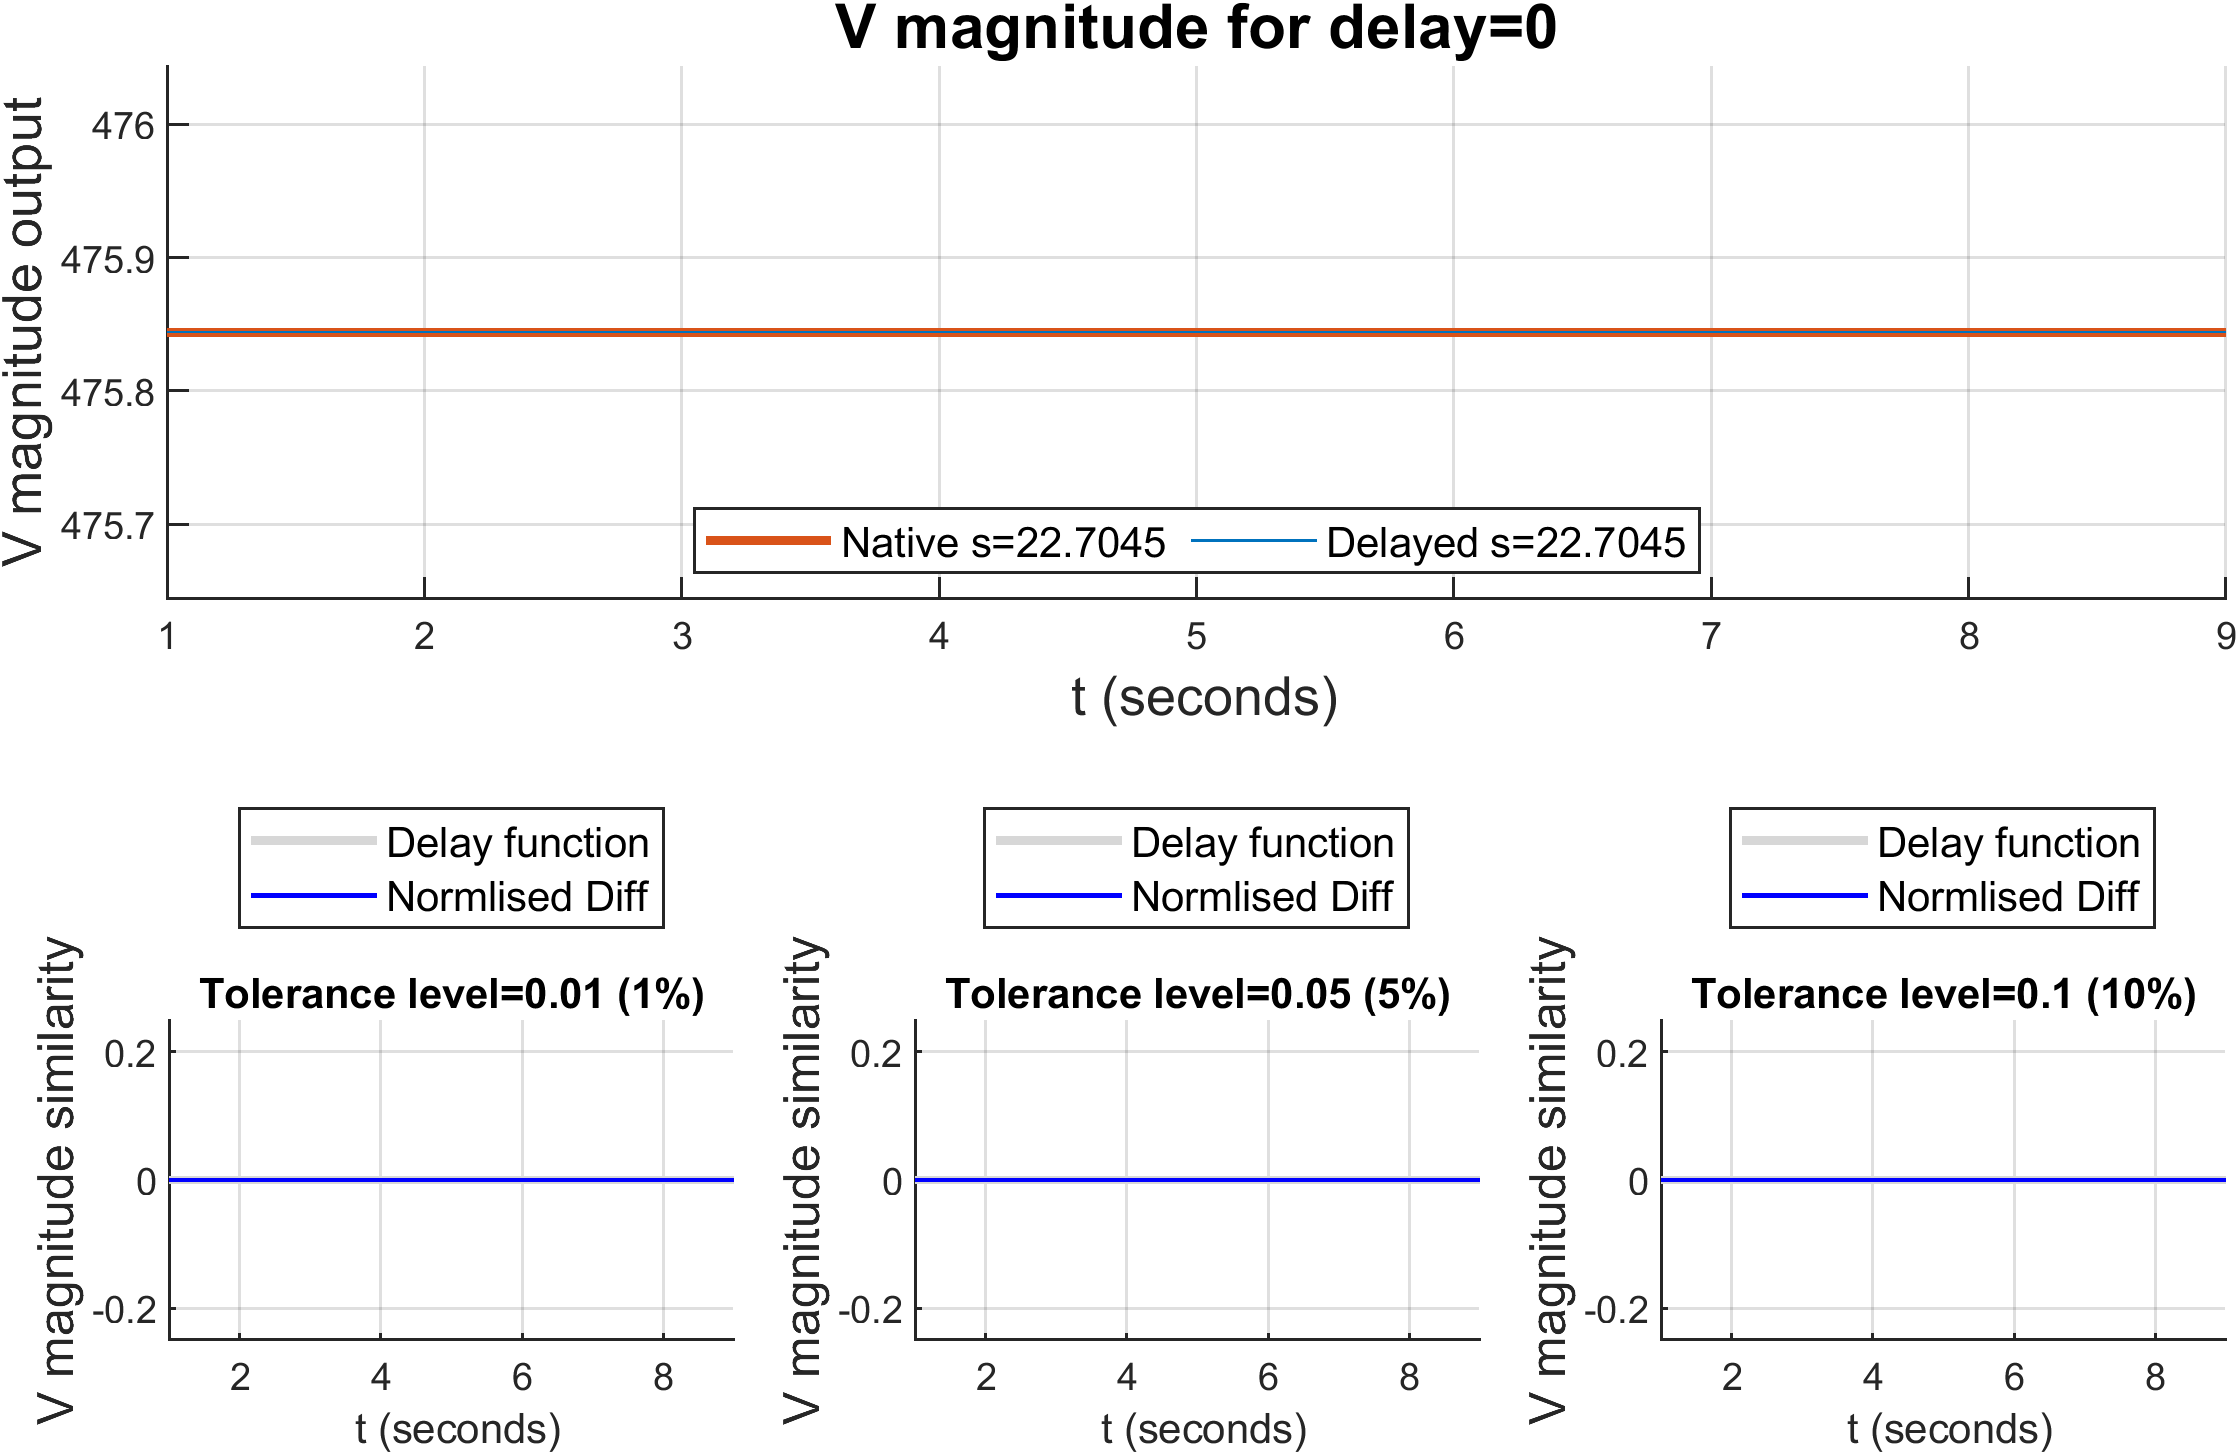
\includegraphics[width=0.95\textwidth]{PMUsim-figures/DelayOf_0/Zero_vMagnitude.png}} \\ 
   
   \fbox{    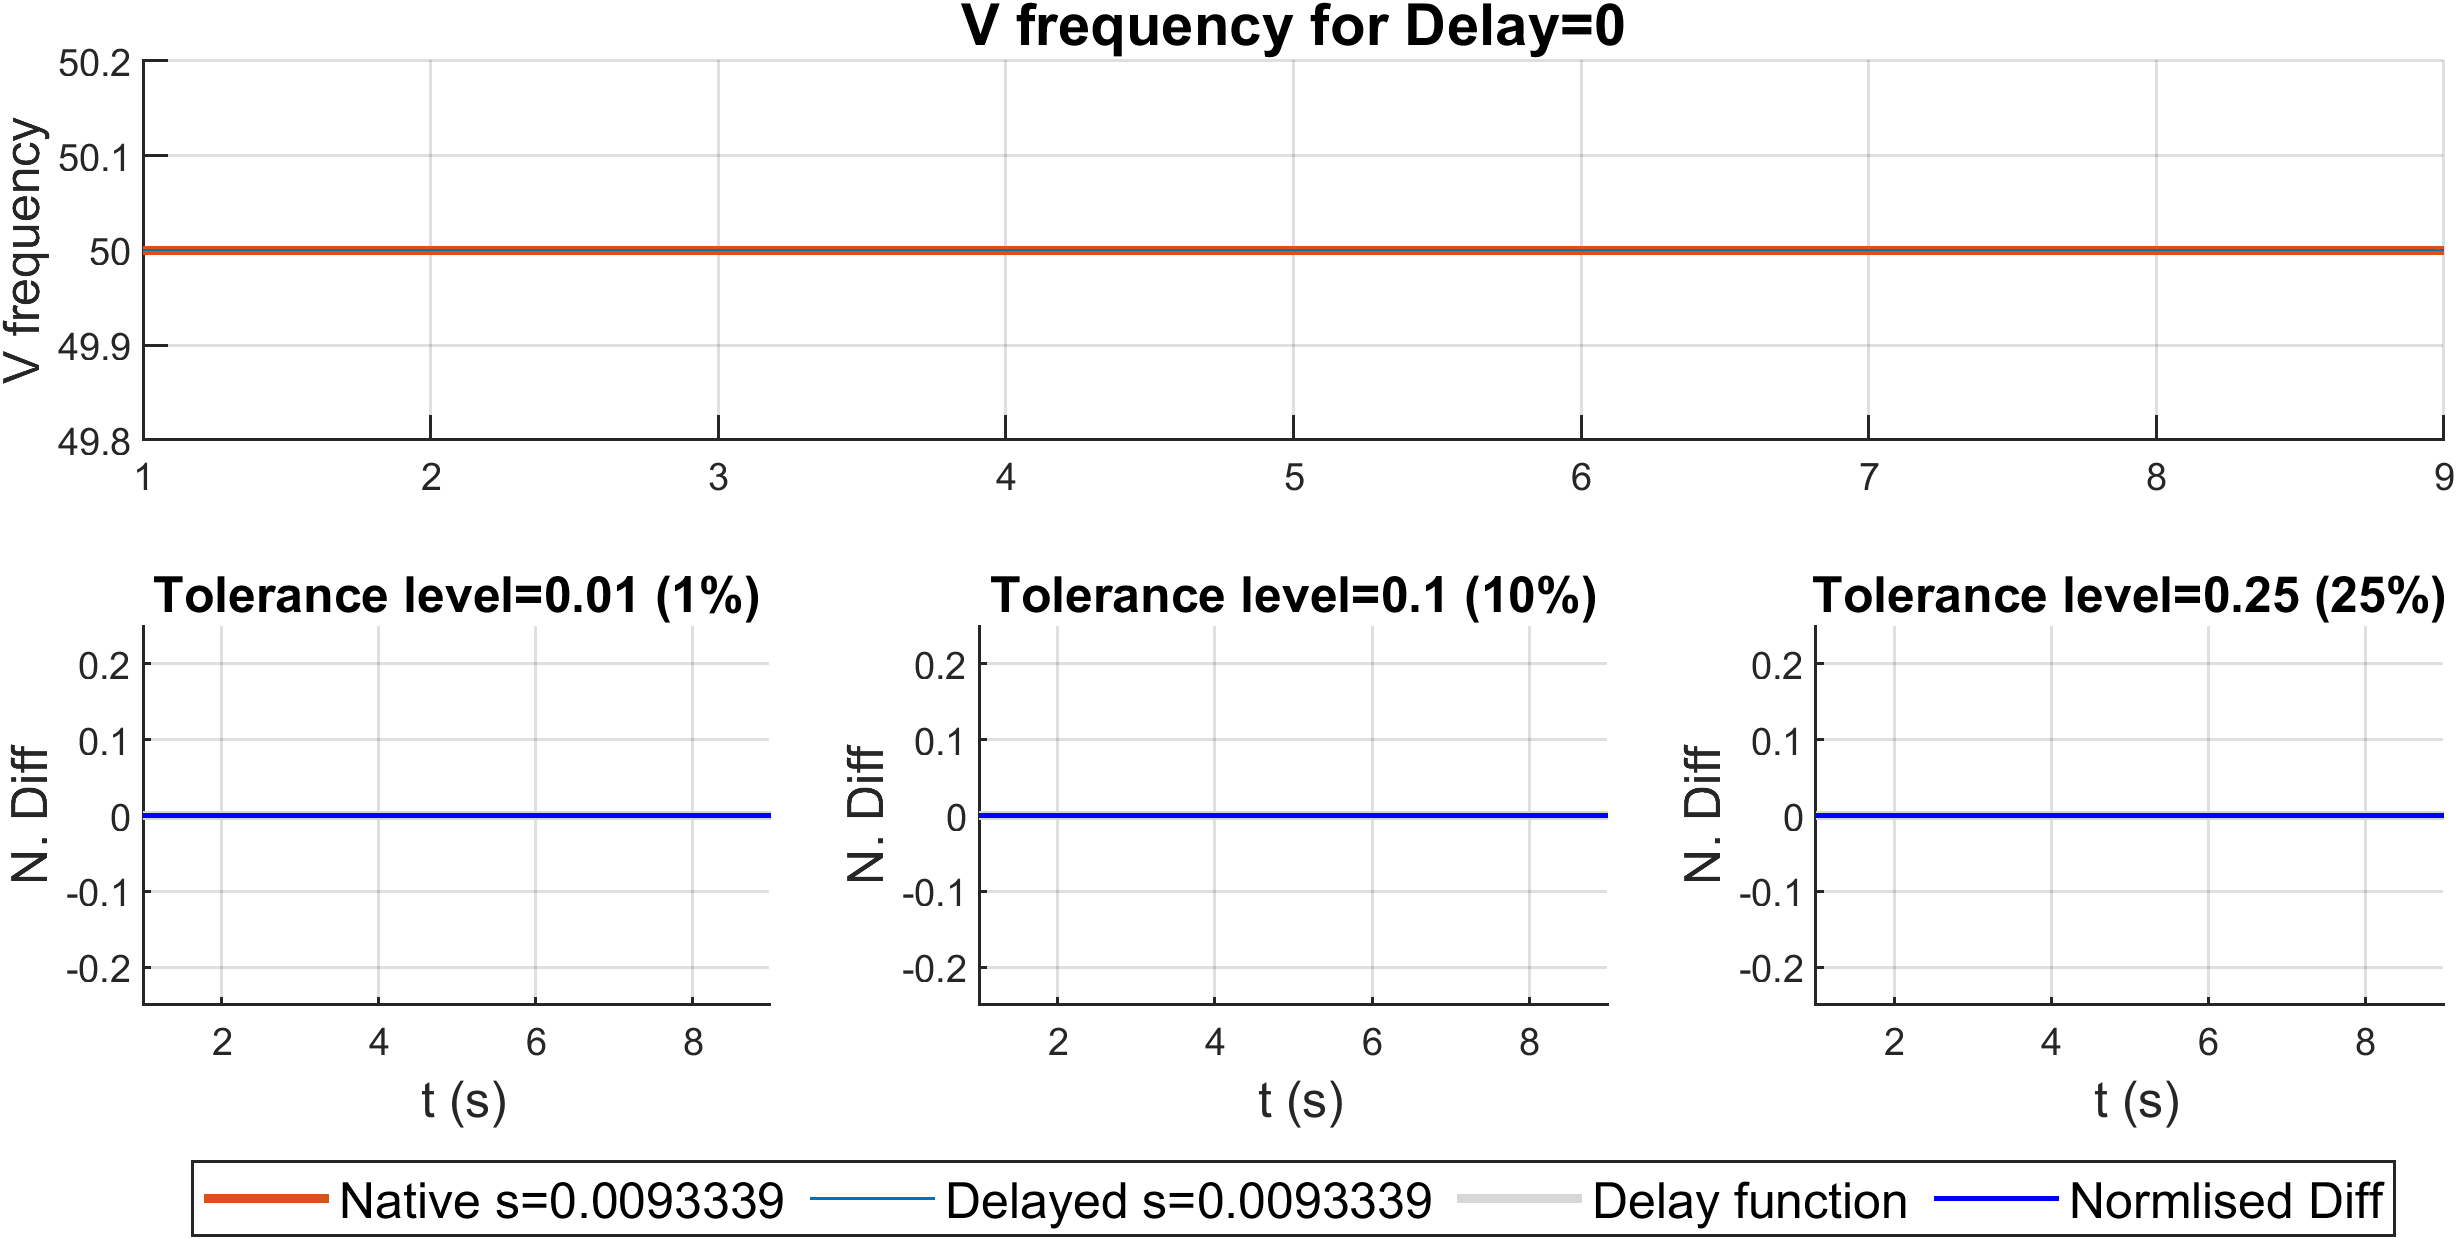
\includegraphics[width=0.95\textwidth]{PMUsim-figures/DelayOf_0/Zero_vFrequency.png}} \\ 

   \fbox{     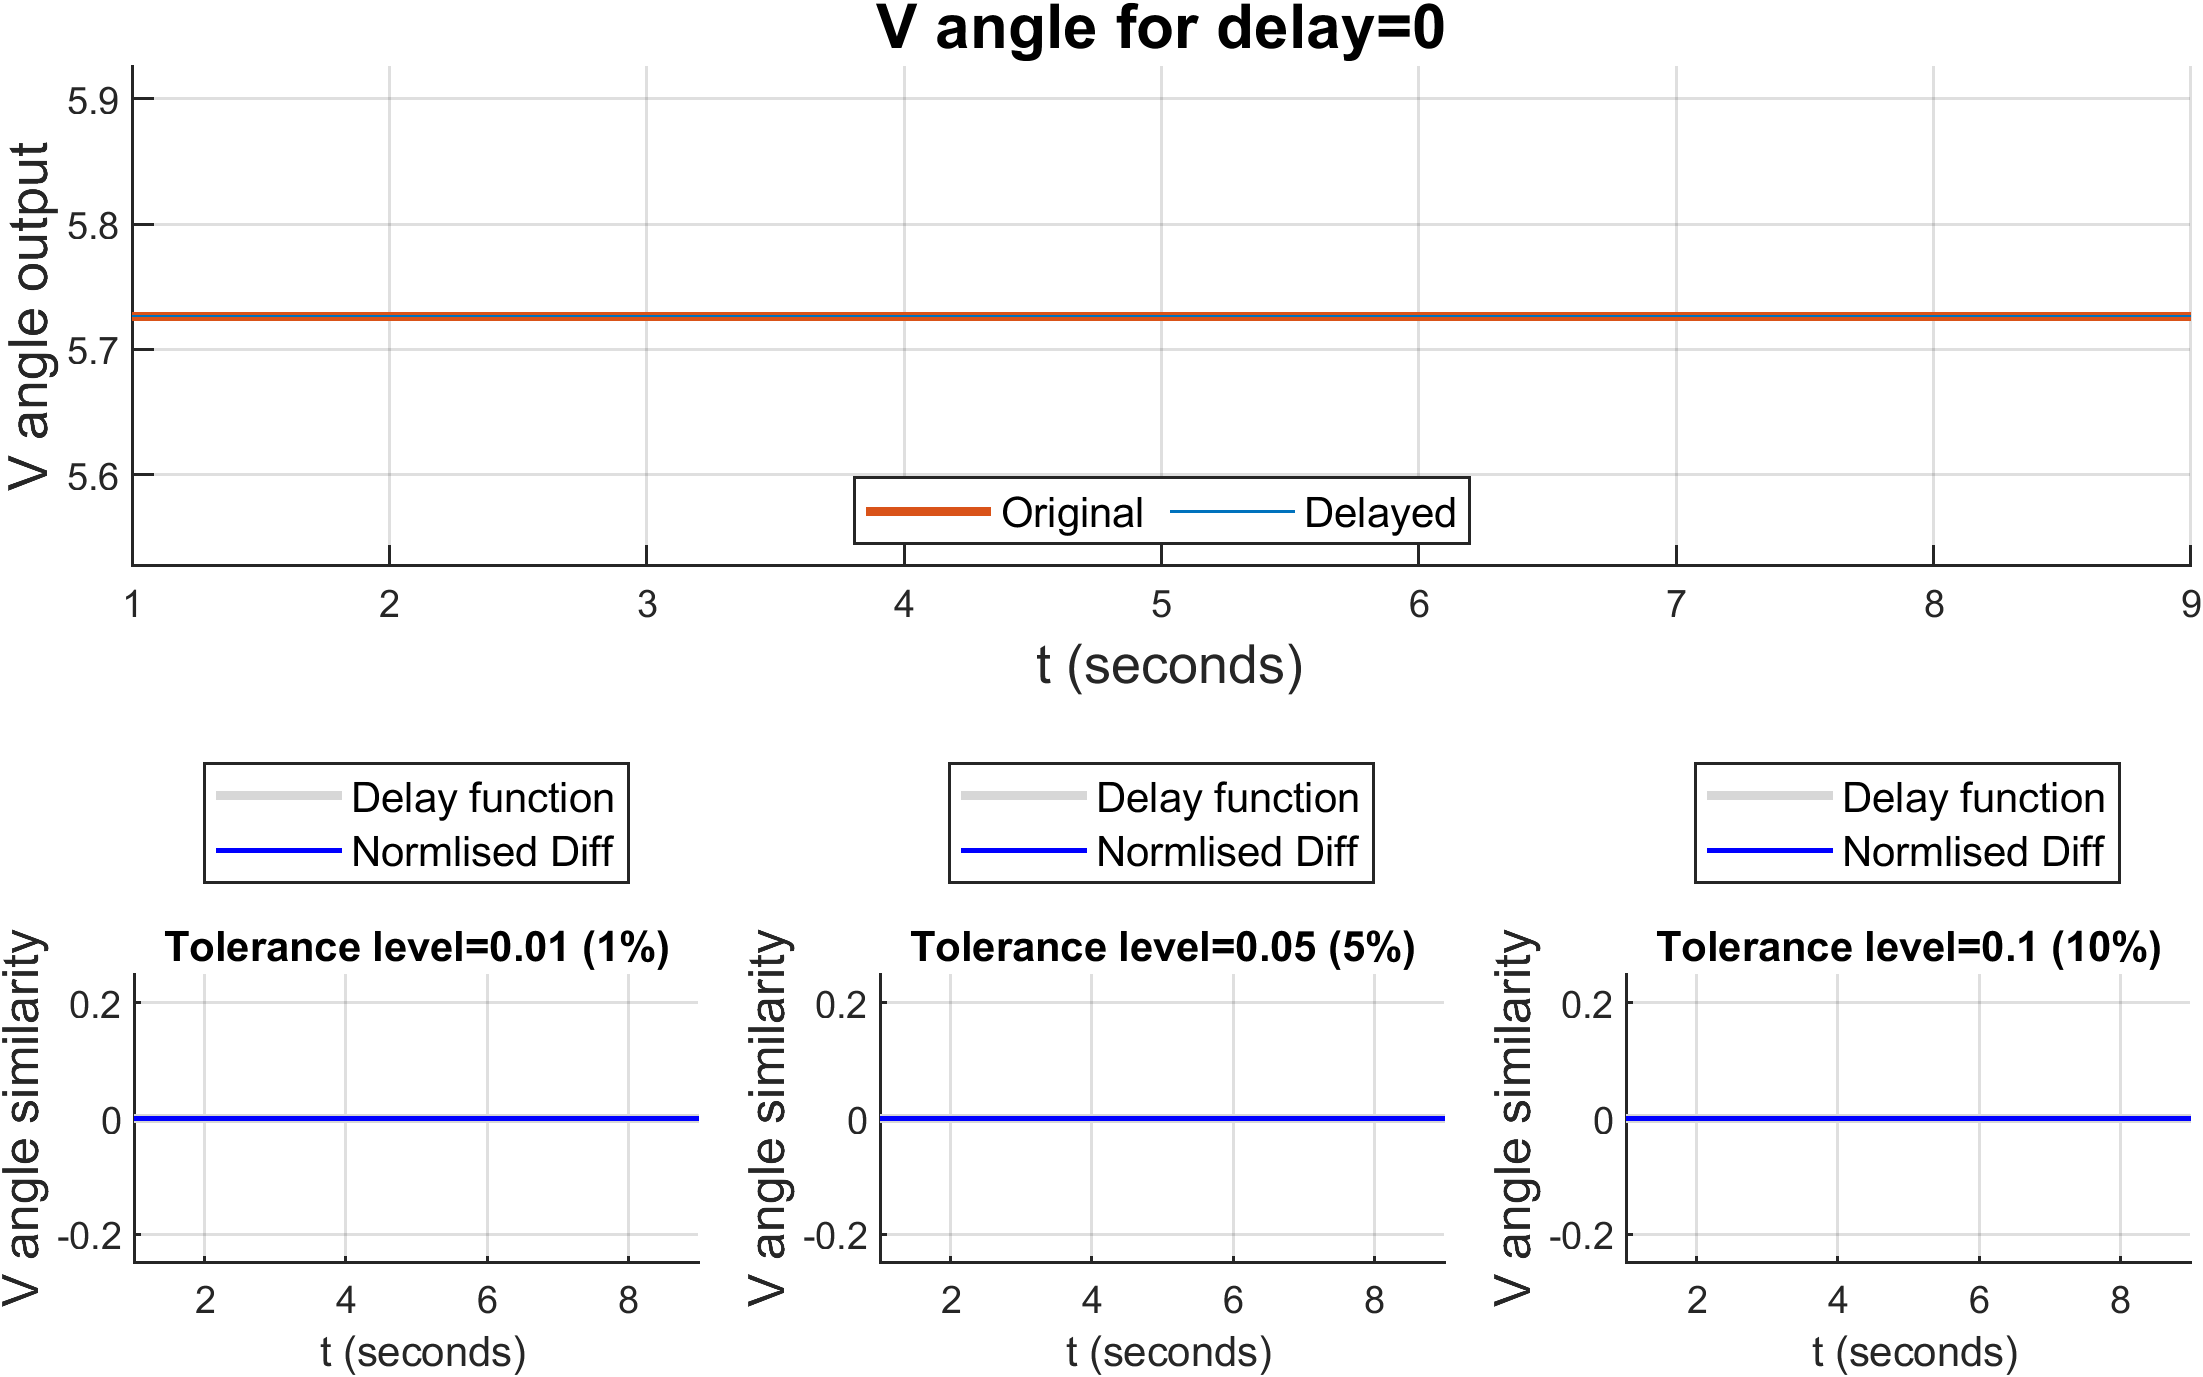
\includegraphics[width=0.95\textwidth]{PMUsim-figures/DelayOf_0/Zero_vAngle.png}}

  \end{tabular}
\label{fig:VoltageZeroDelay}
\caption{Results for Voltage Output for Delay equal to Zero }
\end{figure}



\newpage
\begin{figure}[H]
\begin{tabular}{c}
    \fbox{ 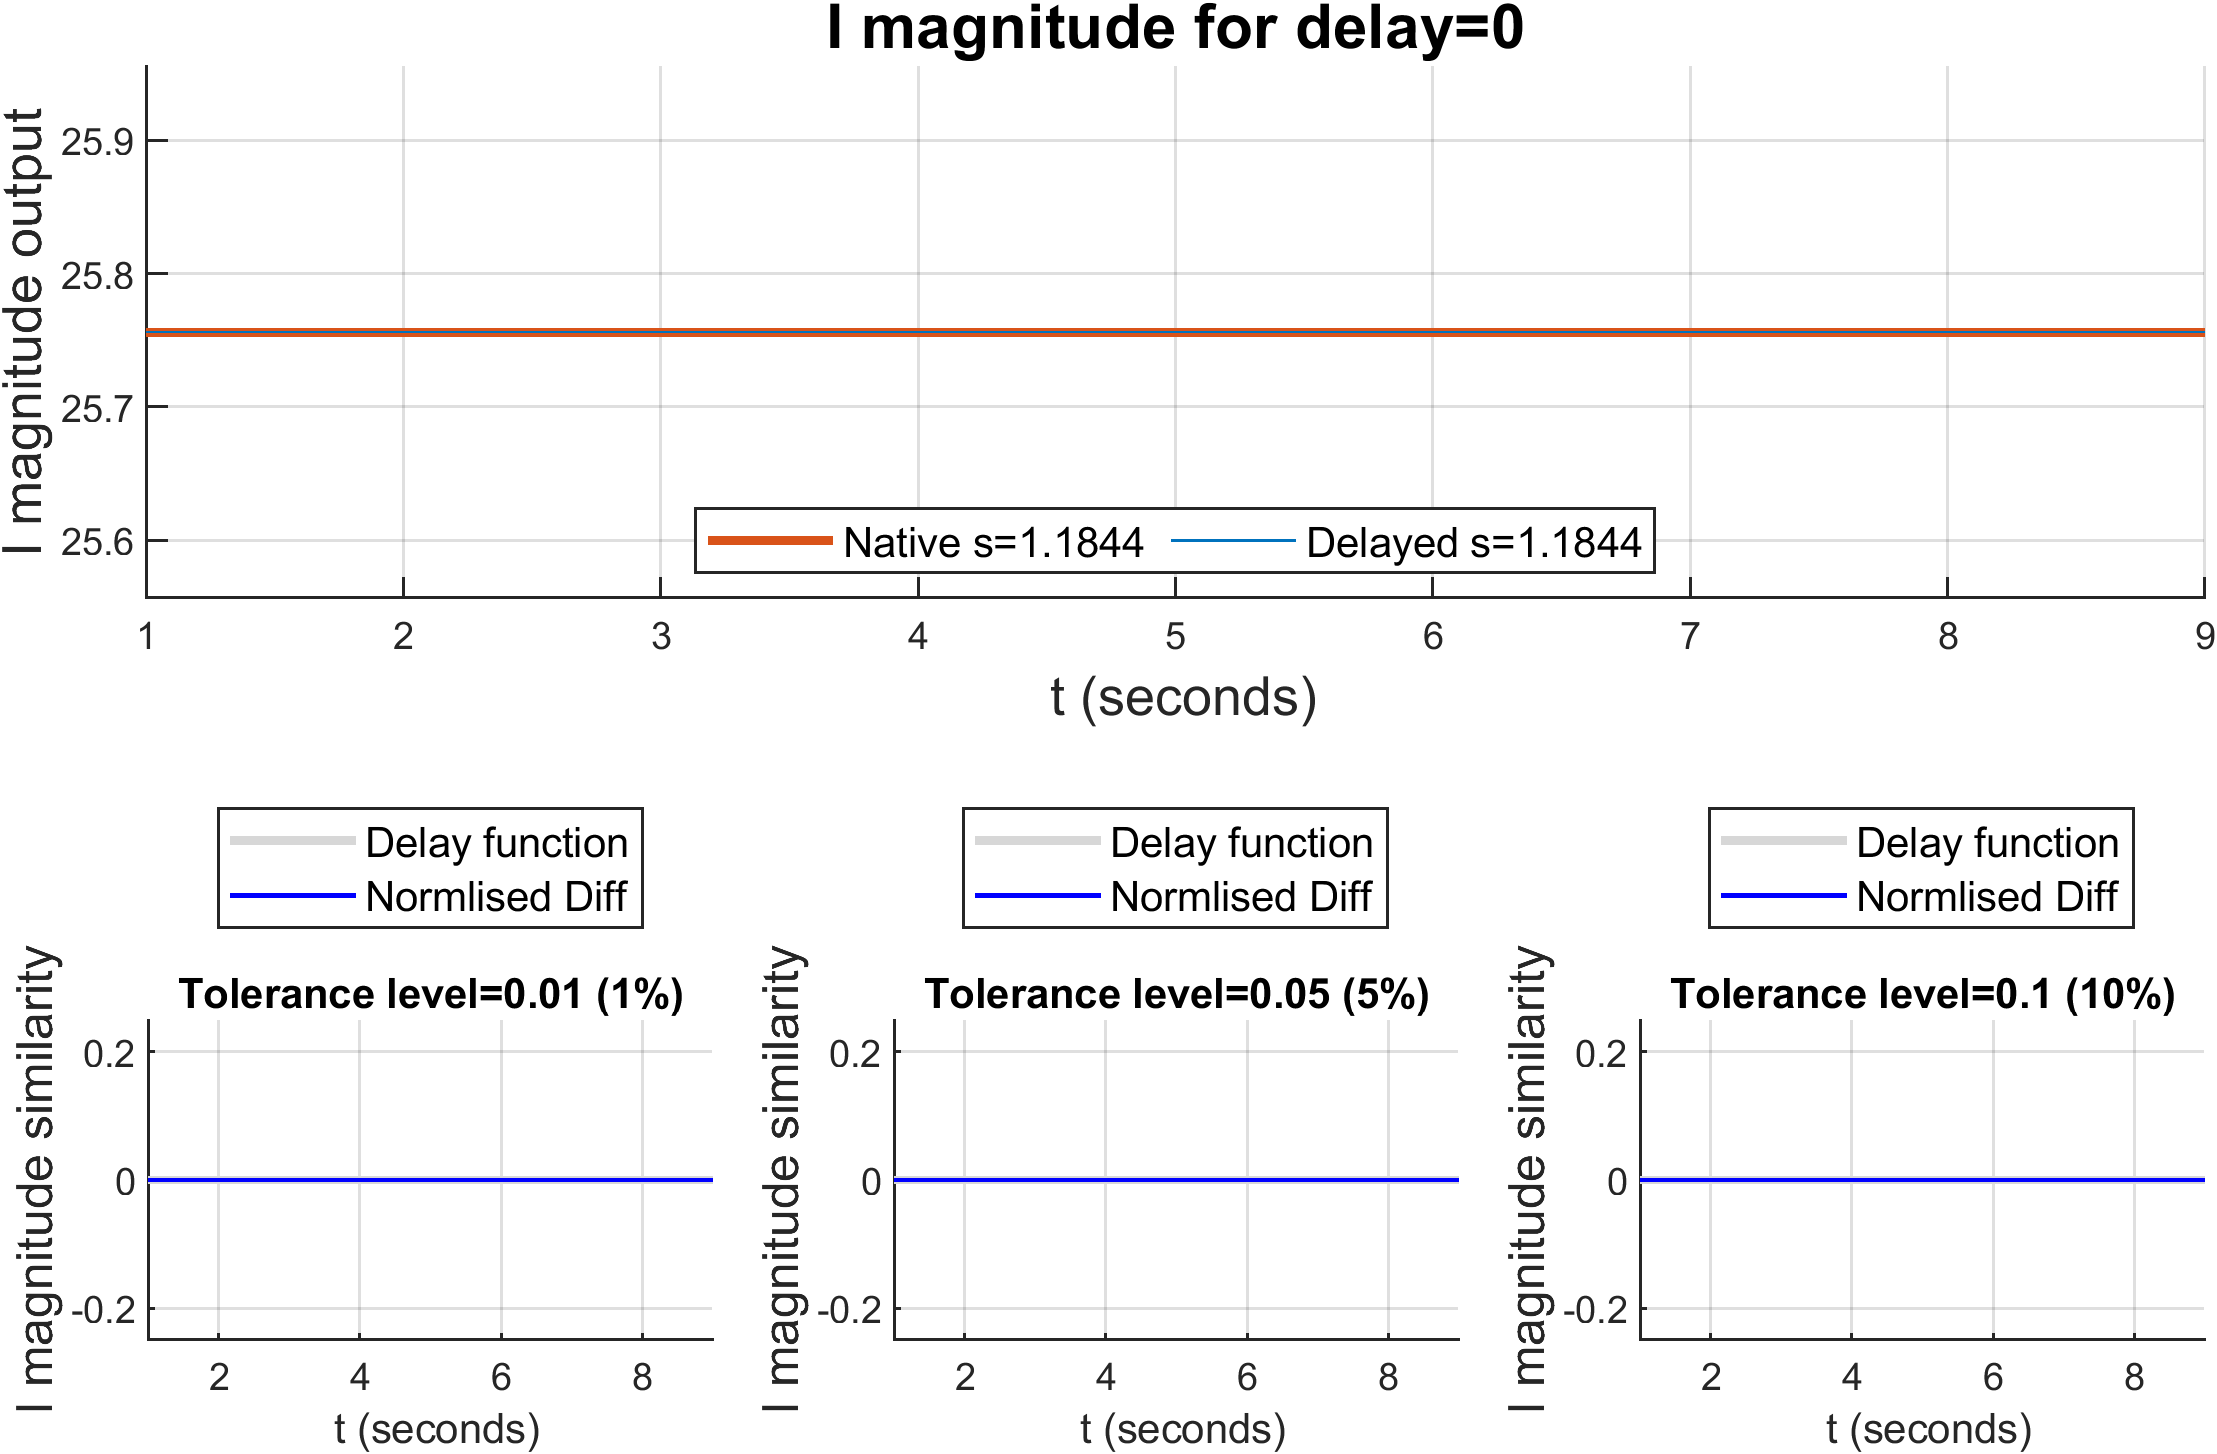
\includegraphics[width=0.95\textwidth]{PMUsim-figures/DelayOf_0/Zero_iMagnitude.png}} \\
	
       \fbox{ 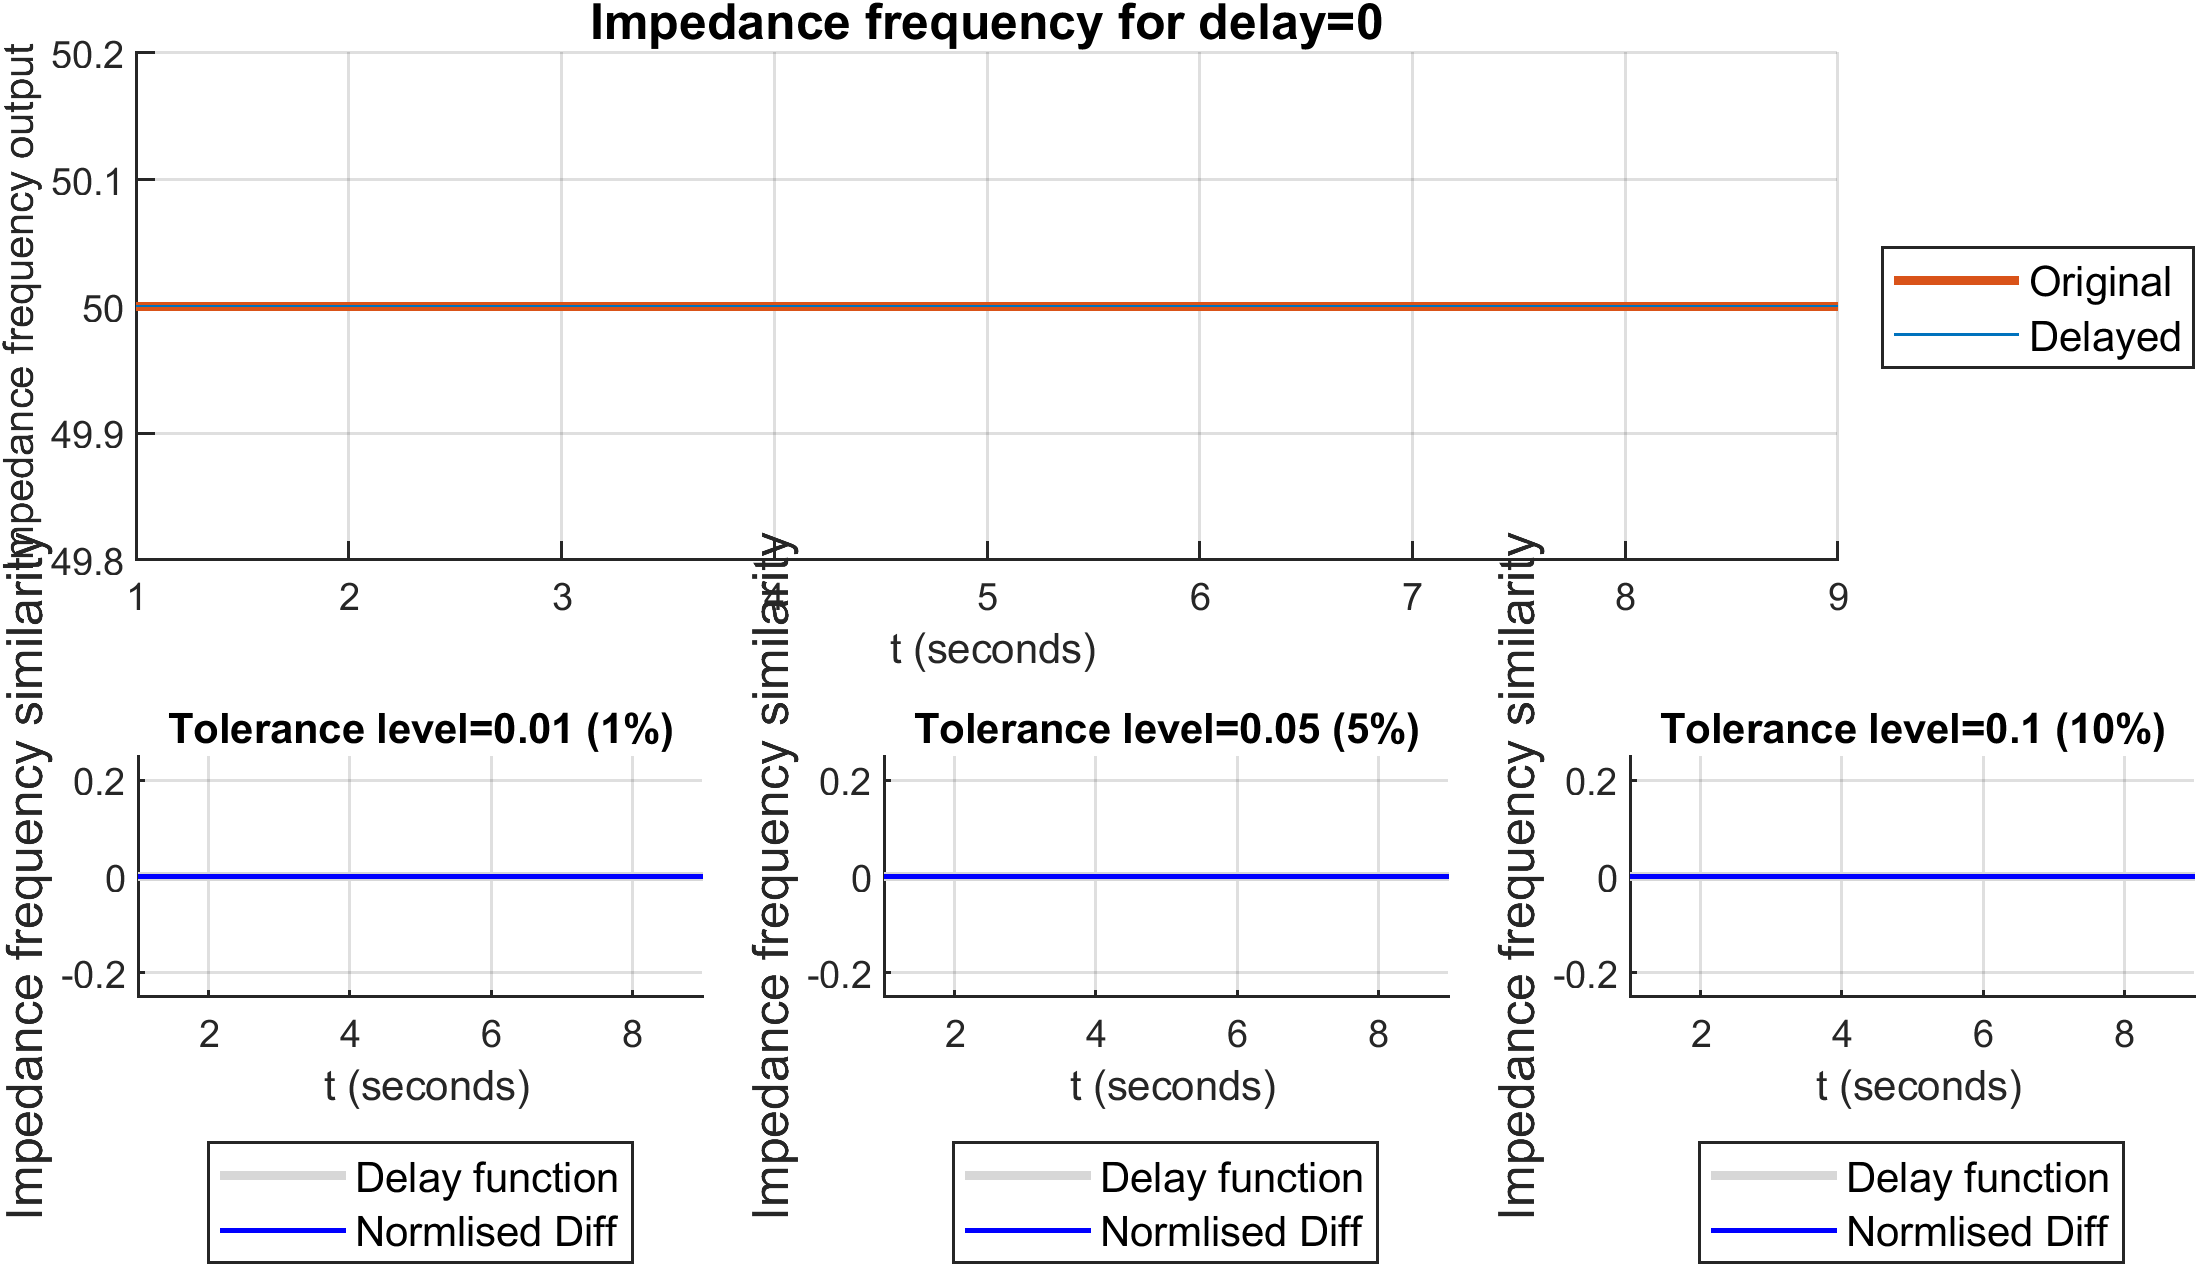
\includegraphics[width=0.95\textwidth]{PMUsim-figures/DelayOf_0/Zero_iFrequency.png}}  \\
	   
   \fbox{  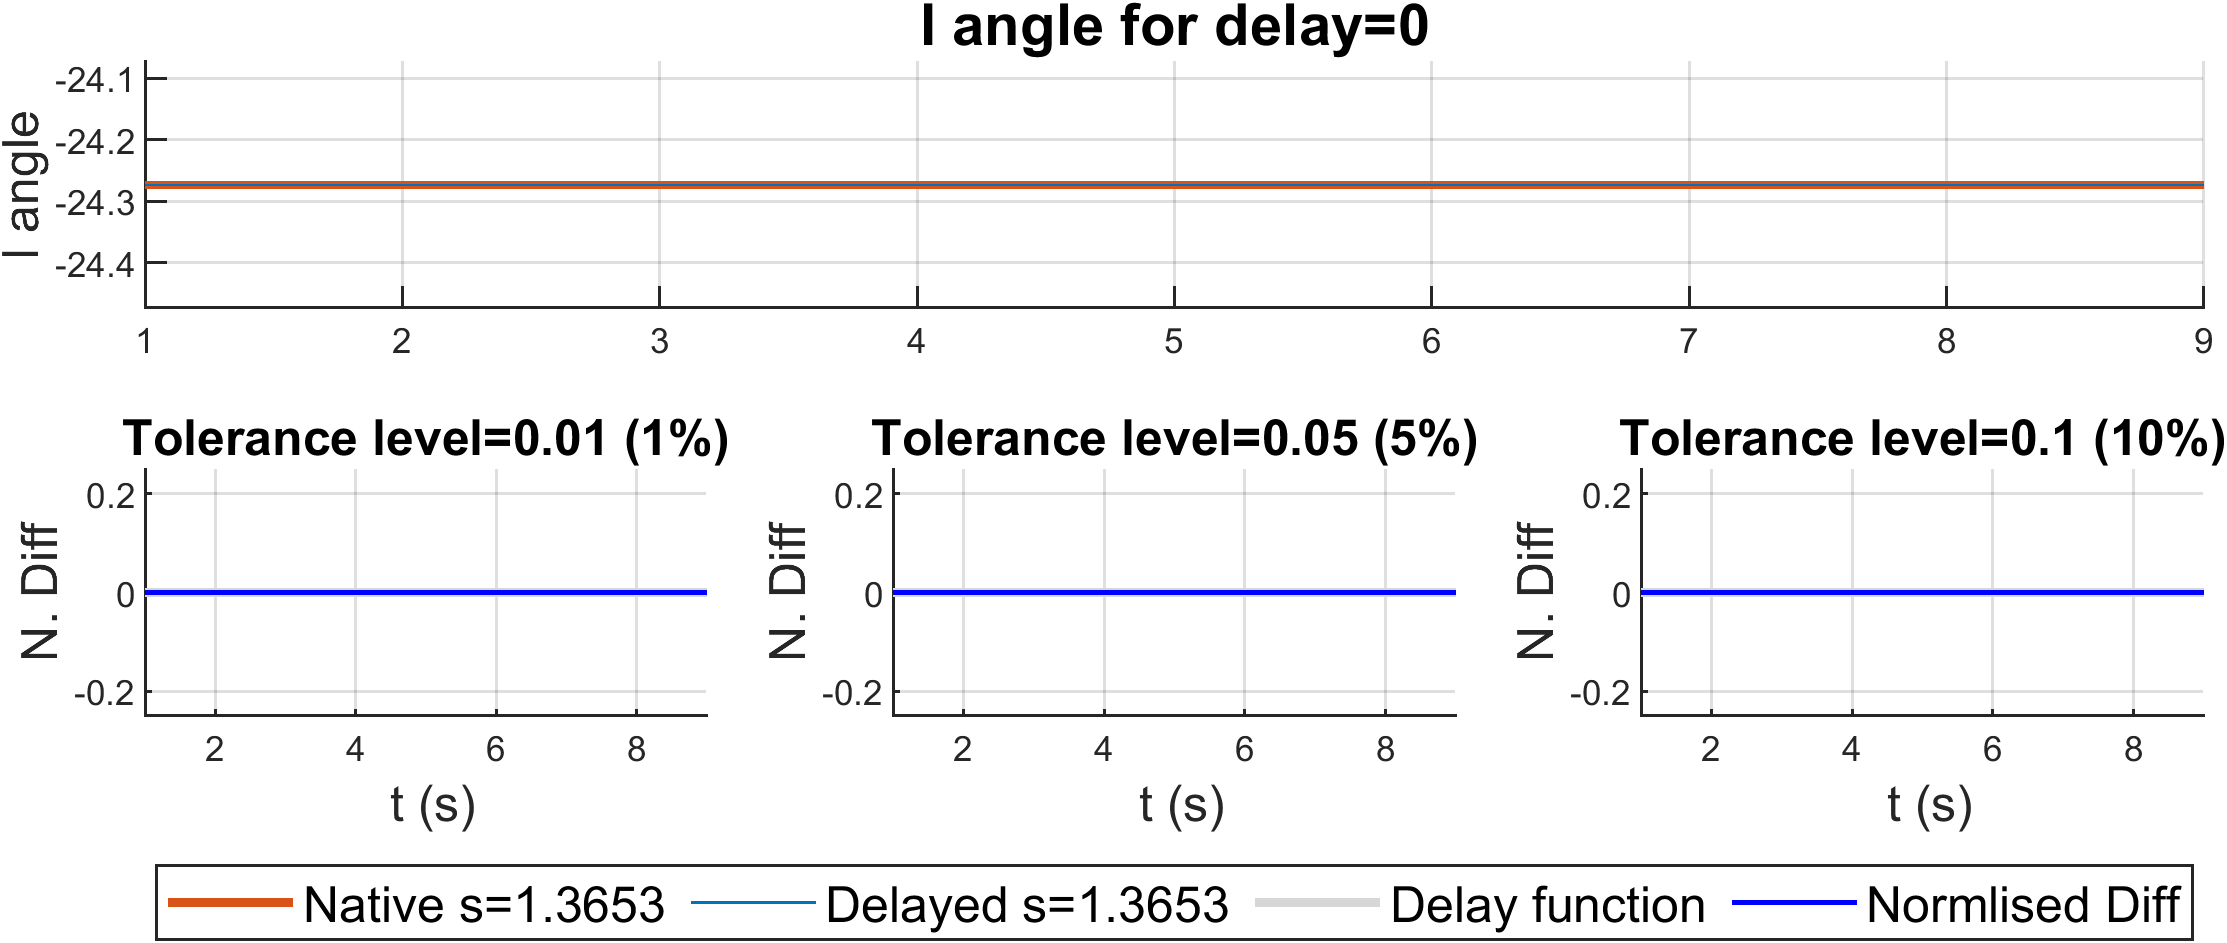
\includegraphics[width=0.95\textwidth]{PMUsim-figures/DelayOf_0/Zero_iAngle.png}} \\ 


 %\caption{Zero Delay Frequency Output (for the Delay Level of Zero)}
  \end{tabular}
\label{fig:ImpedanceZeroDelay}
\caption{Results for Impedance Output for Delay equal to Zero }
\end{figure}






\section{The Delay Level of One}
For model verification purposes, the output for the delay level of zero is included.

\begin{small}
     \tcbox[size=normal, standard jigsaw, opacityback=0, boxrule=0pt,halign=justify]{
     Comment on the figure for Instant delay of One}{
          \begin{itemize}
         \item   
         \item  
          \end{itemize} 
}
\end{small}







\section{Instant Delay Functions}

\subsection{Instant Delay Level of One}

\subsection{Instant Delay Level of Two}

\subsection{Instant Delay Level of Three}

\subsection{Instant Delay Level of Four}

\subsection{Instant Delay Level of Five}

\subsection{Instant Delay Level of Six}






\section{Step-Wise Delay functions}


\subsection{Step-Wise Delay Level of Two}

\subsection{Step-Wise Delay Level of Three}

\subsection{Step-Wise Delay Level of Four}

\subsection{Step-Wise Delay Level of Five}

\subsection{Step-Wise Delay Level of Six}



\newpage
\begin{figure}[H]
\begin{tabular}{c}
  \fbox{  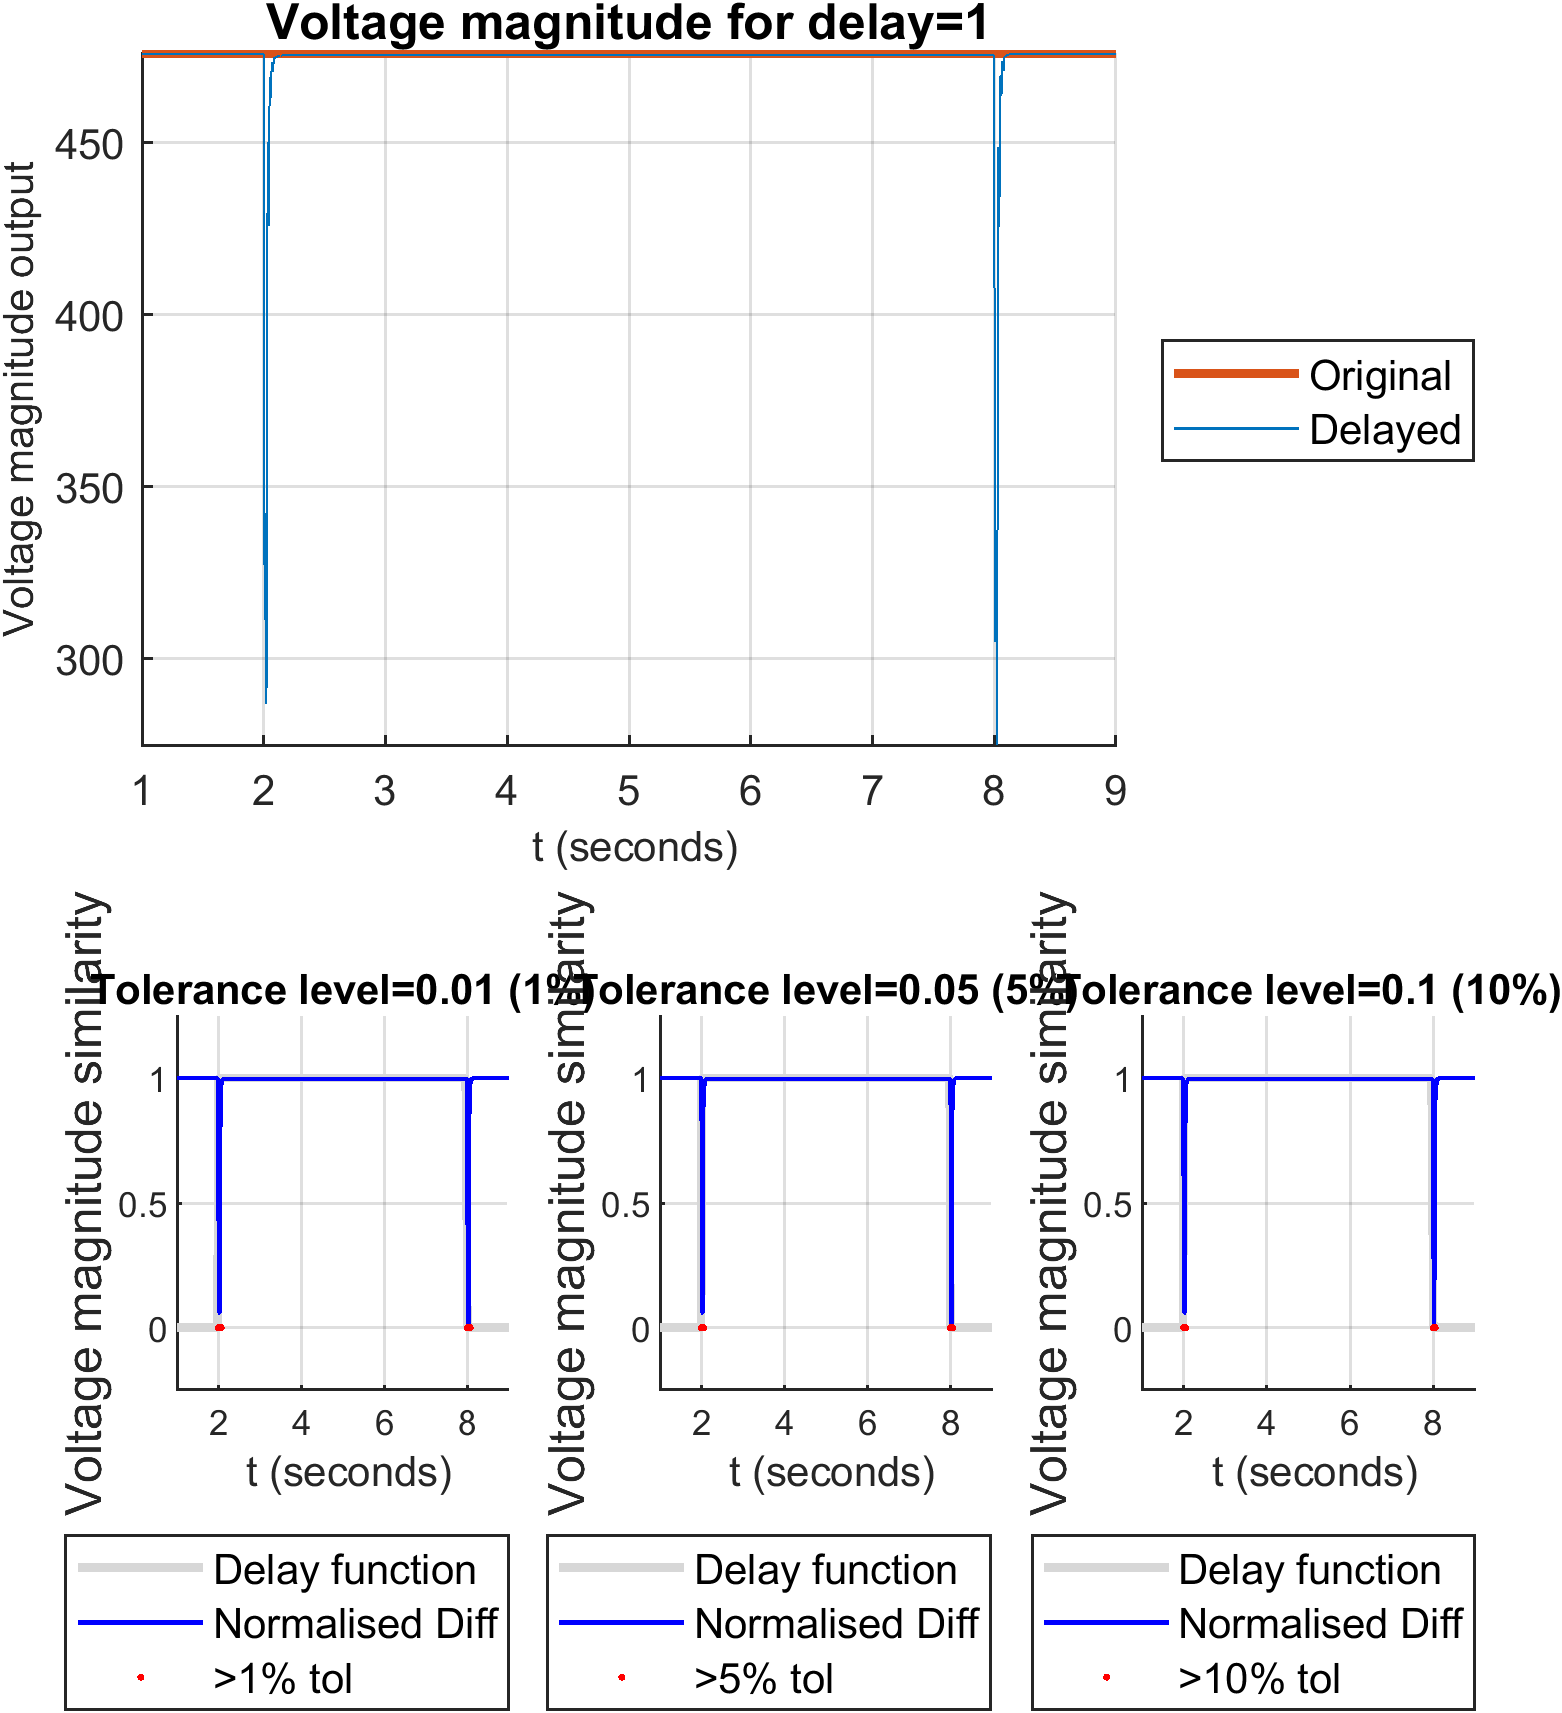
\includegraphics[width=0.95\textwidth]{PMUsim-figures/DelayOf_1/Instant_vMagnitude.png}} \\ 
   \fbox{     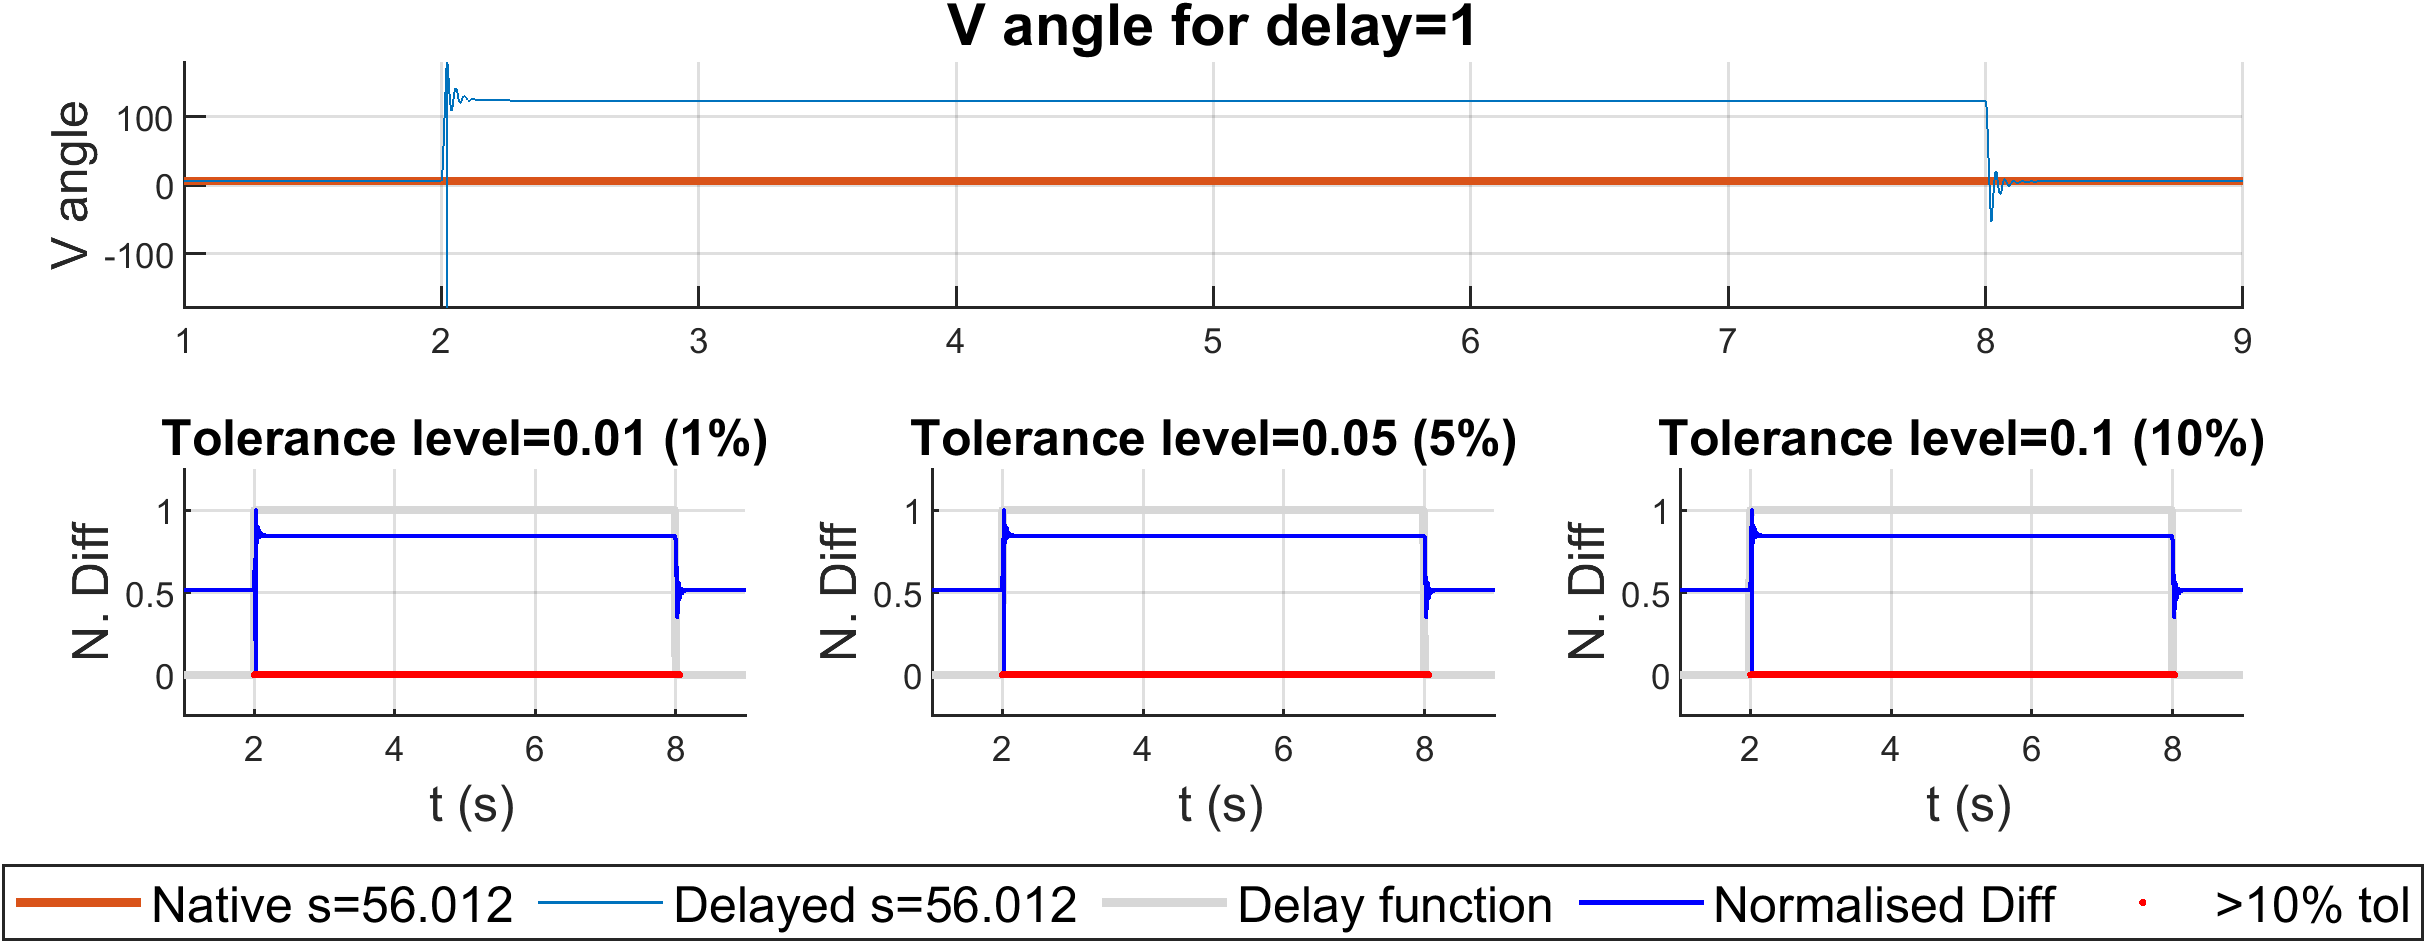
\includegraphics[width=0.95\textwidth]{PMUsim-figures/DelayOf_1/Instant_vAngle.png}} \\   
   \fbox{    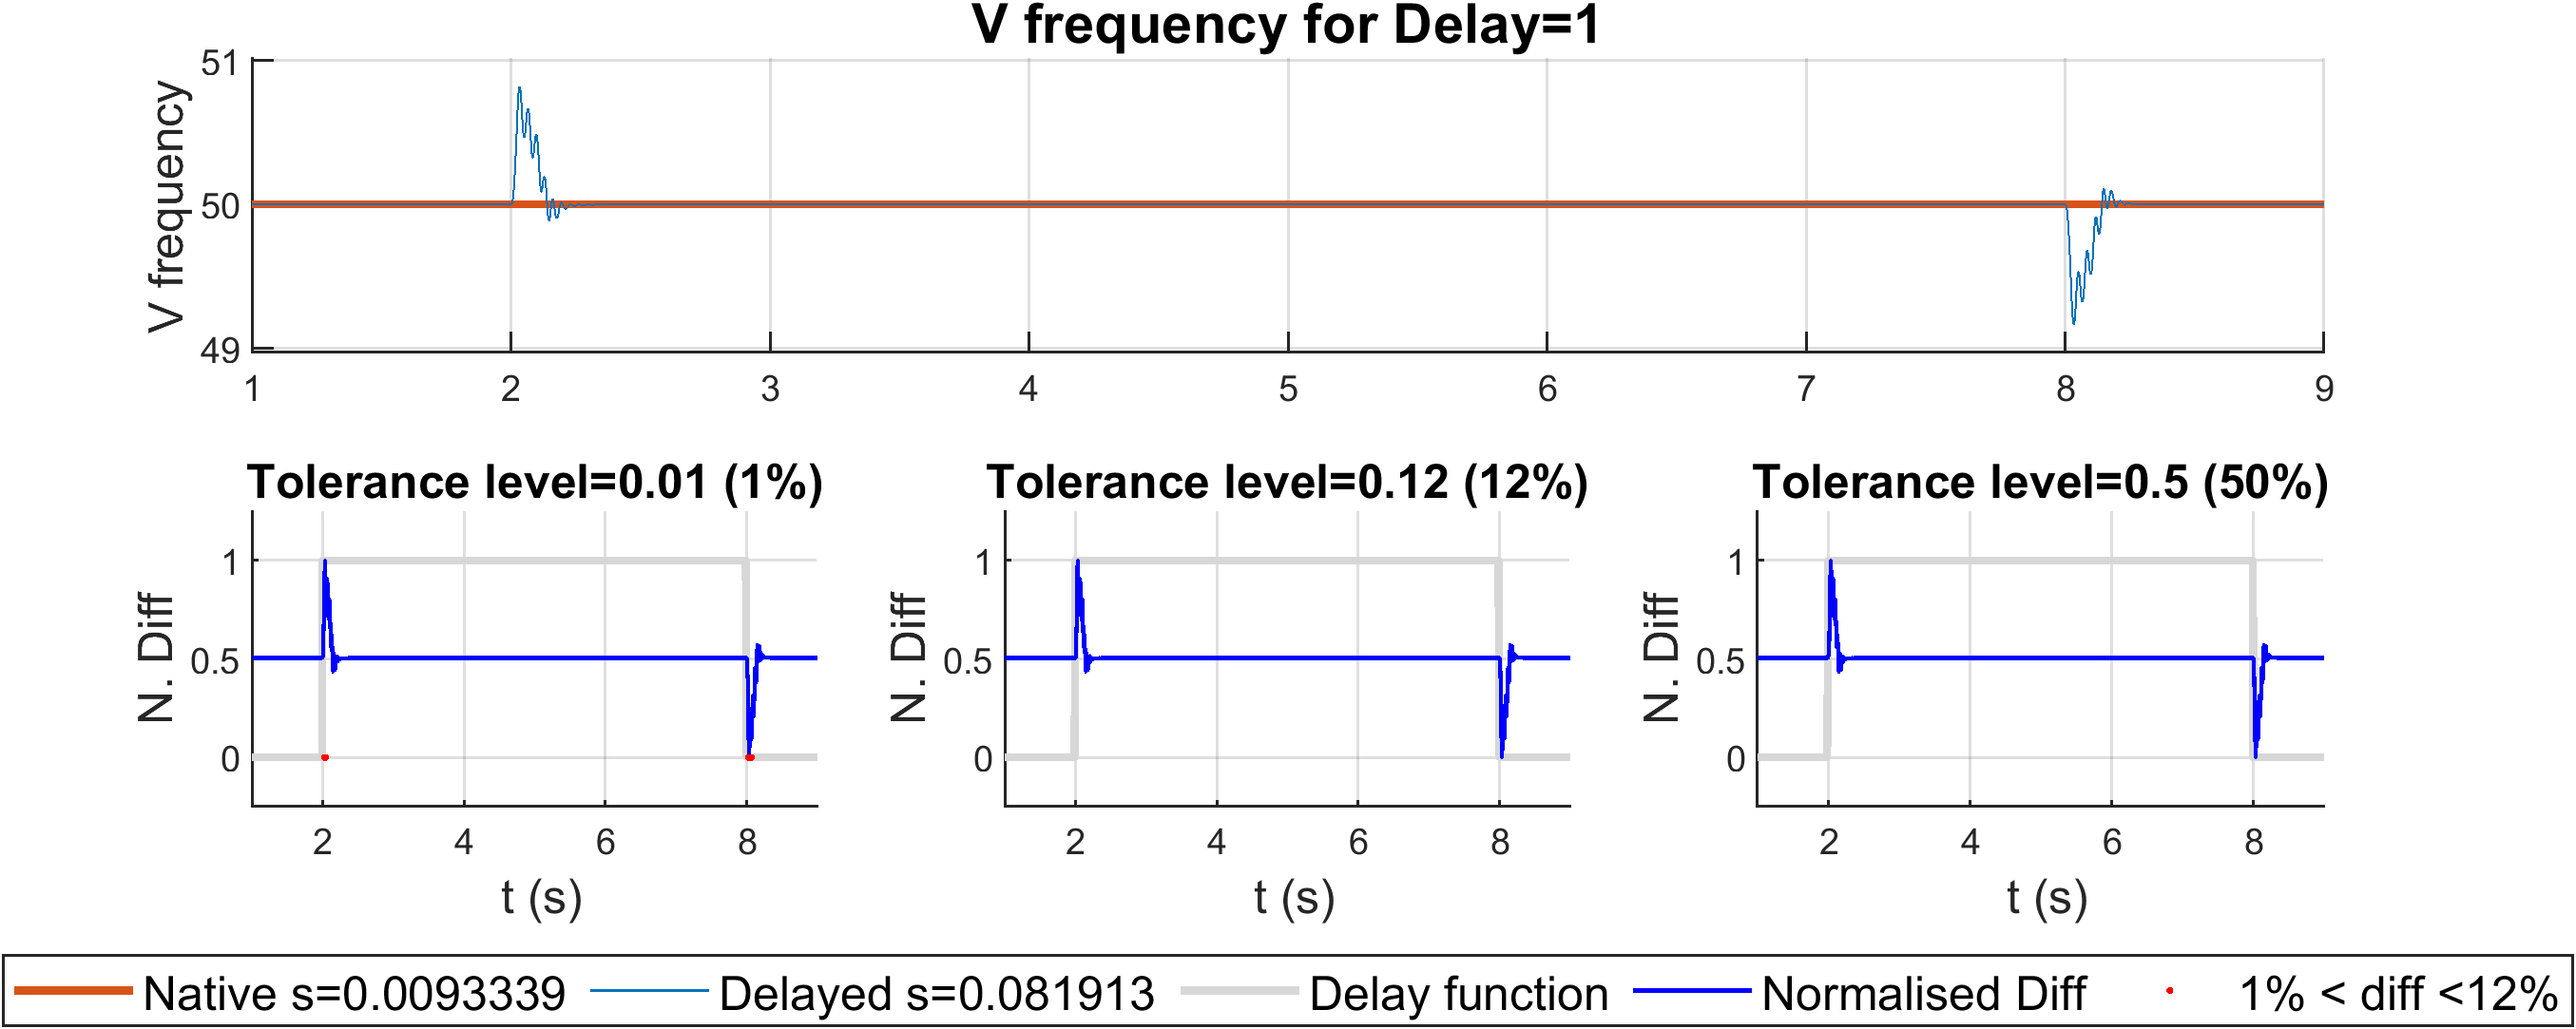
\includegraphics[width=0.95\textwidth]{PMUsim-figures/DelayOf_1/Instant_vFrequency.png}}

 
  \end{tabular}
\caption{Results for Voltage Output for Instant Delay equal to One } 
\label{fig:VoltageInstantDelayOne}
\end{figure}

\newpage
\begin{figure}[H]
\begin{tabular}{c}
  \fbox{  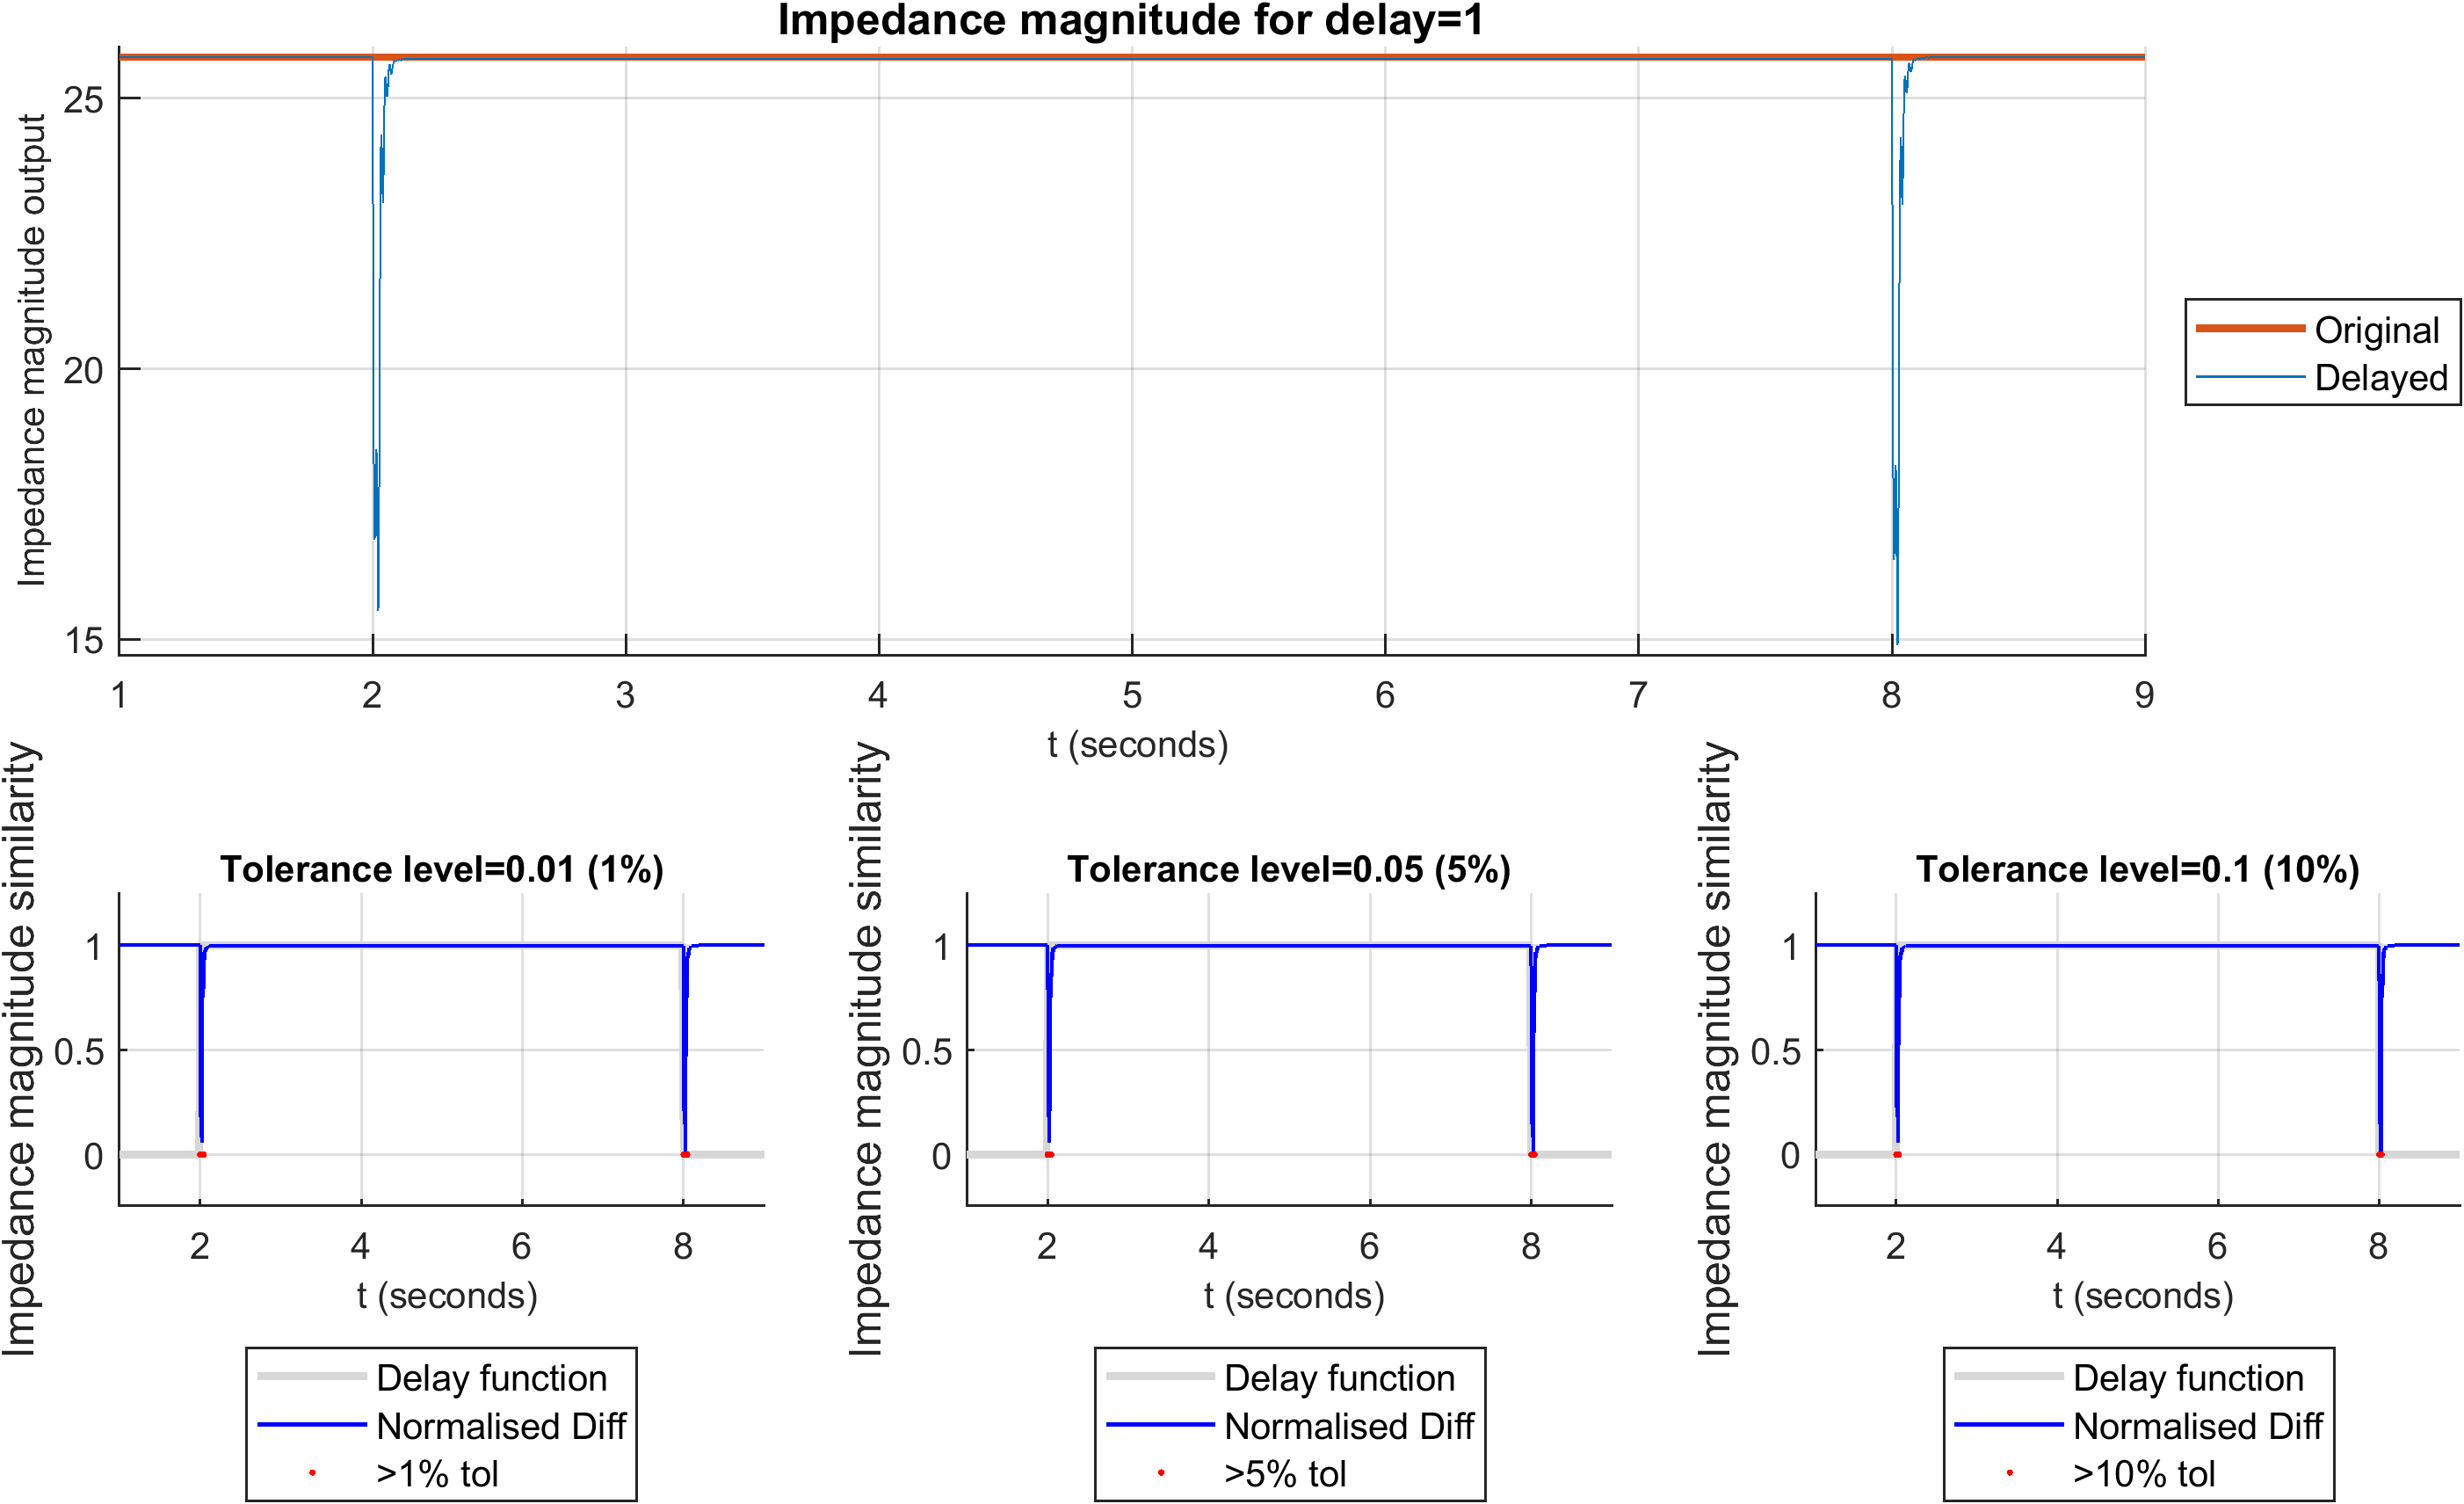
\includegraphics[width=0.95\textwidth]{PMUsim-figures/DelayOf_1/Instant_iMagnitude.png}} \\ 
    \fbox{     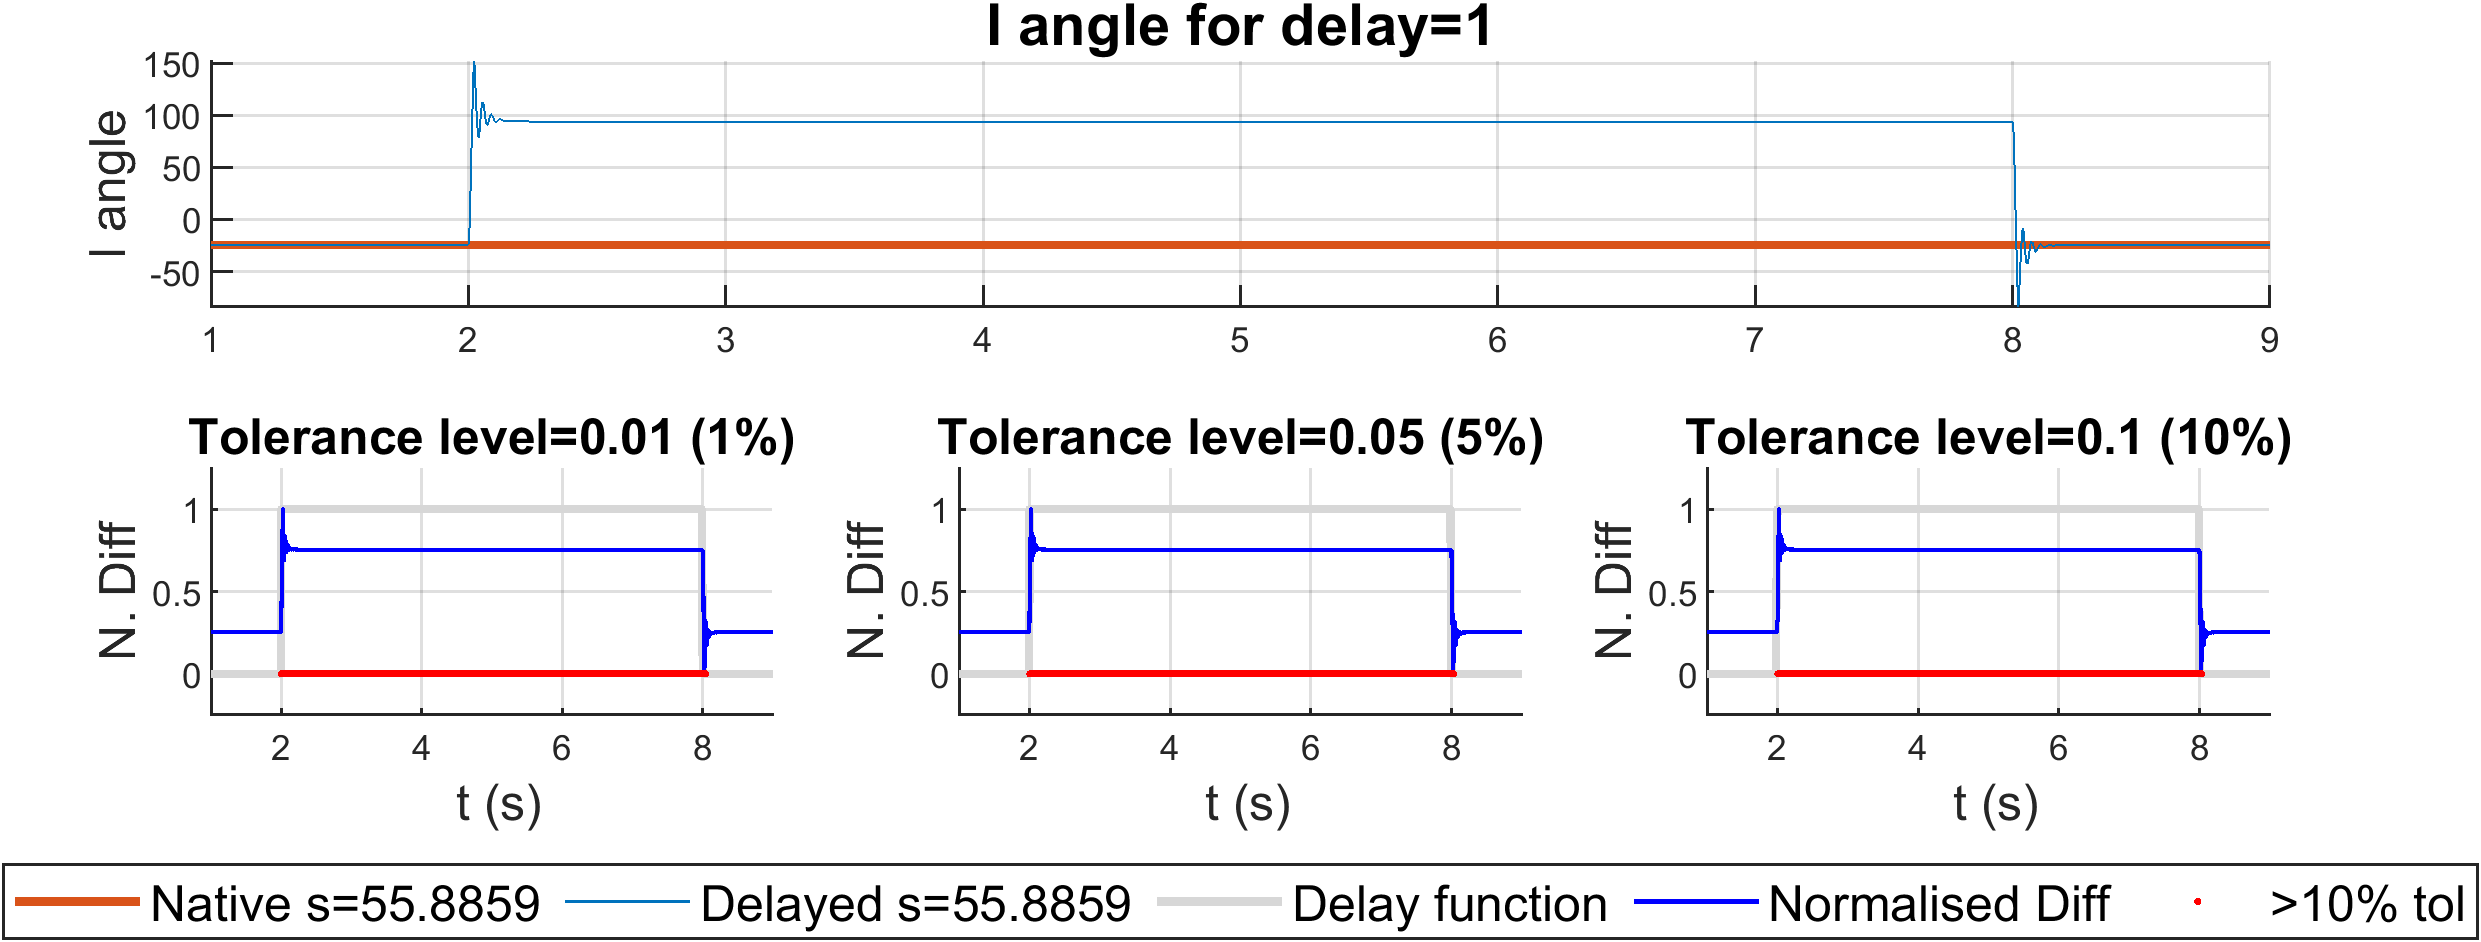
\includegraphics[width=0.95\textwidth]{PMUsim-figures/DelayOf_1/Instant_iAngle.png}} \\   
   \fbox{    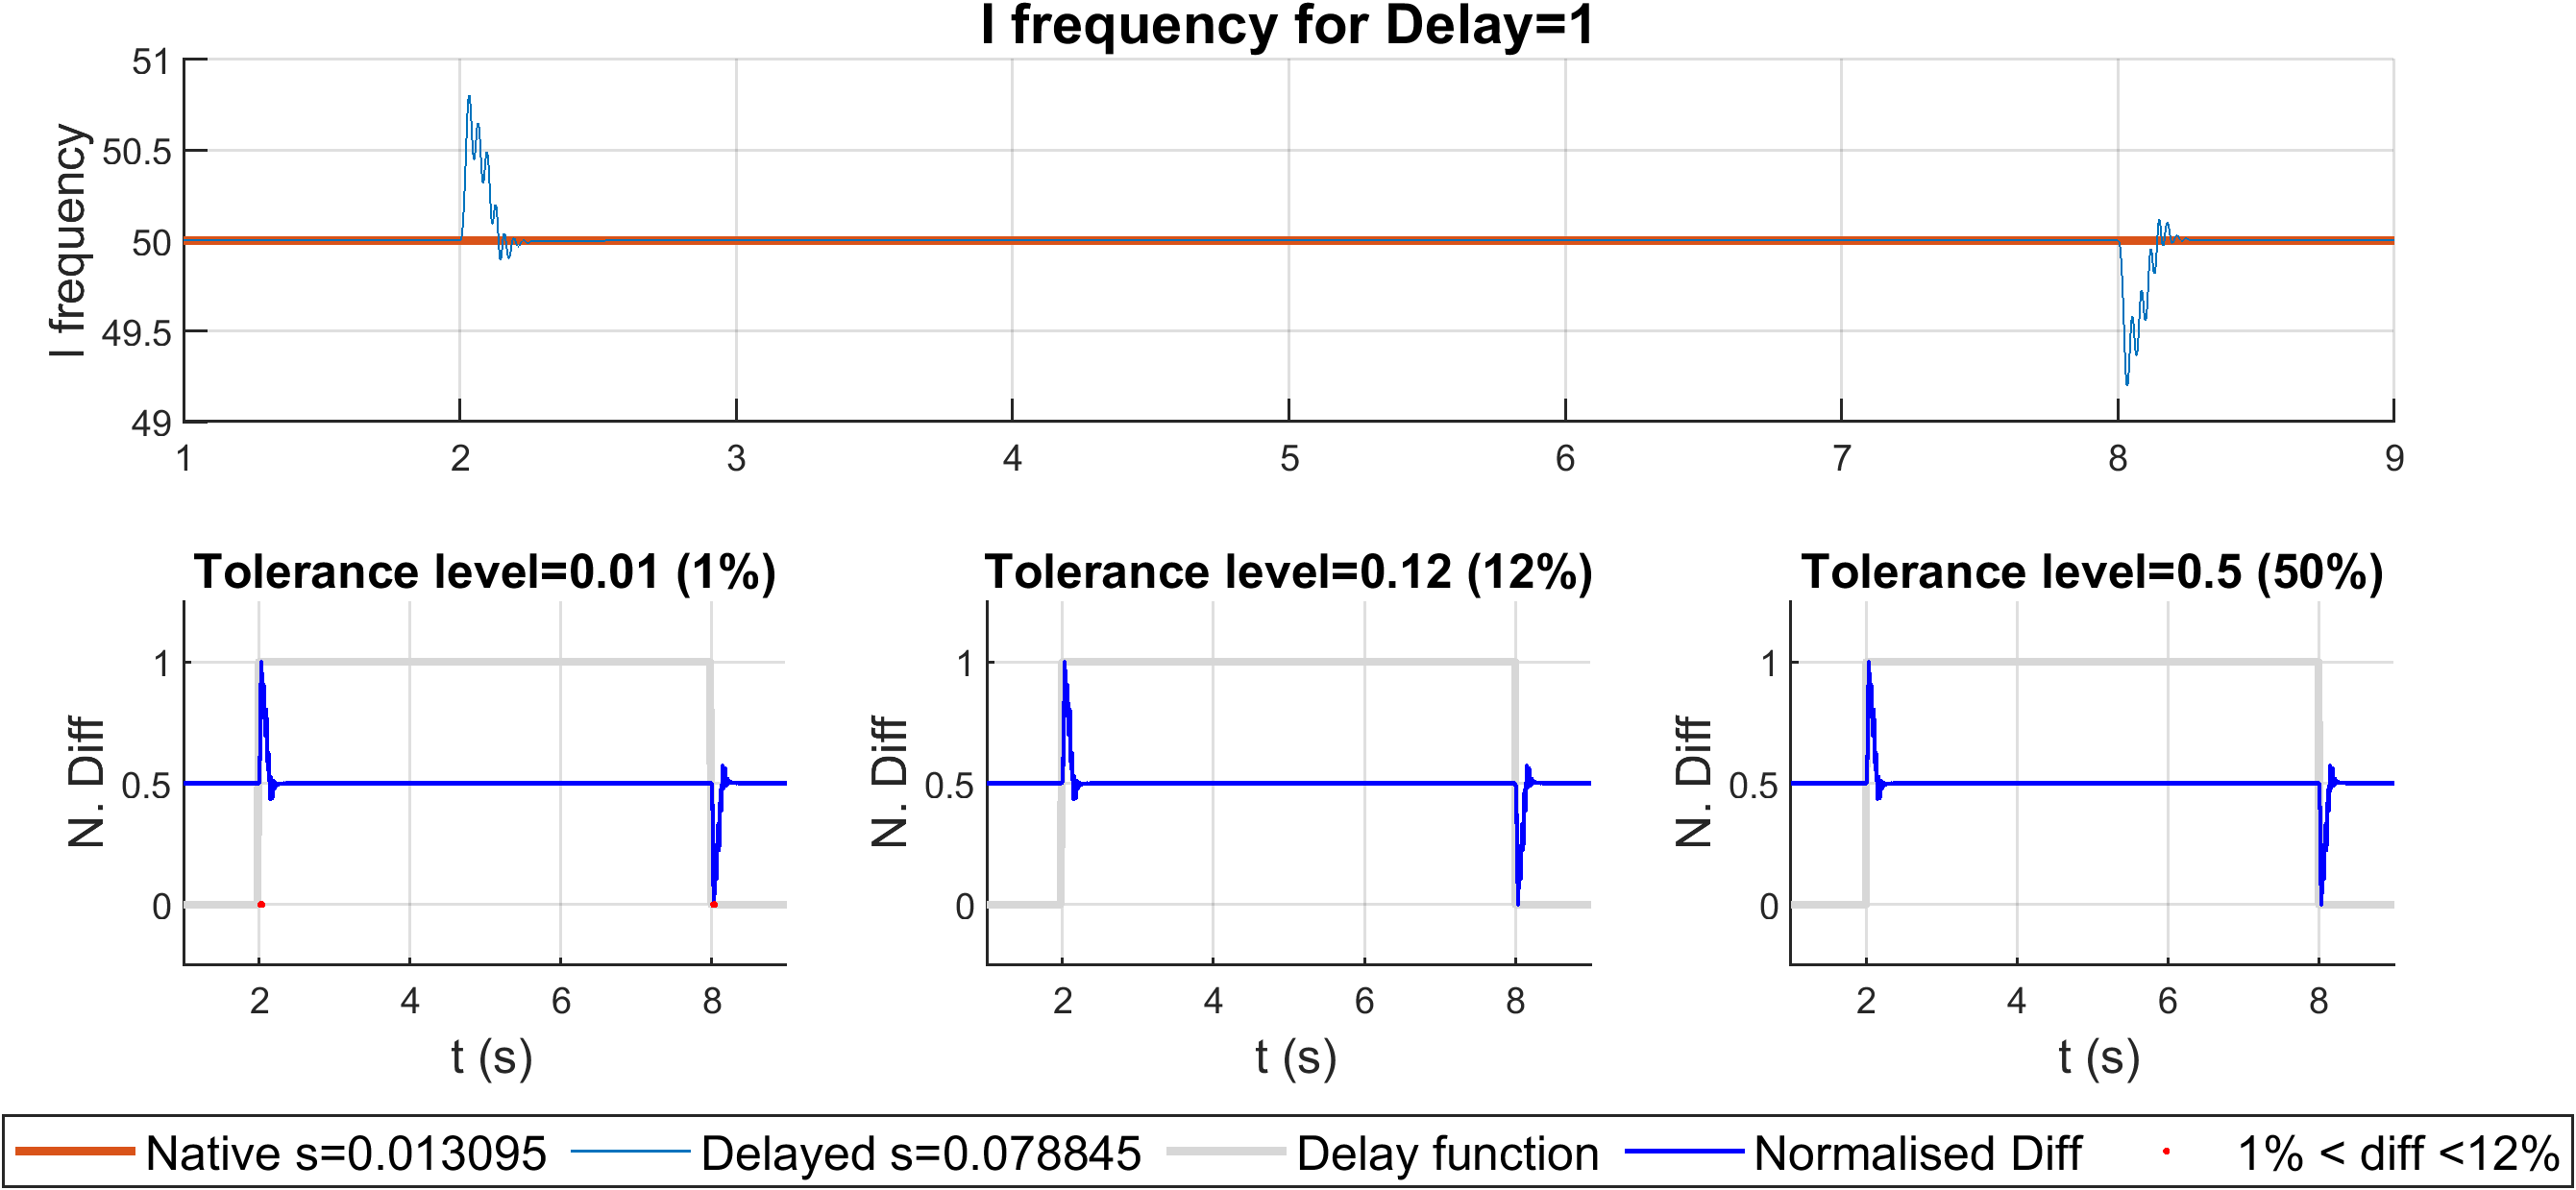
\includegraphics[width=0.95\textwidth]{PMUsim-figures/DelayOf_1/Instant_iFrequency.png}}


  \end{tabular}
\label{fig:ImpedanceInstantDelayOne} 
\caption{Results for Impedance Output for Instant Delay equal to One }
\end{figure}



\newpage
\begin{figure}[H]
\begin{tabular}{c}
  \fbox{  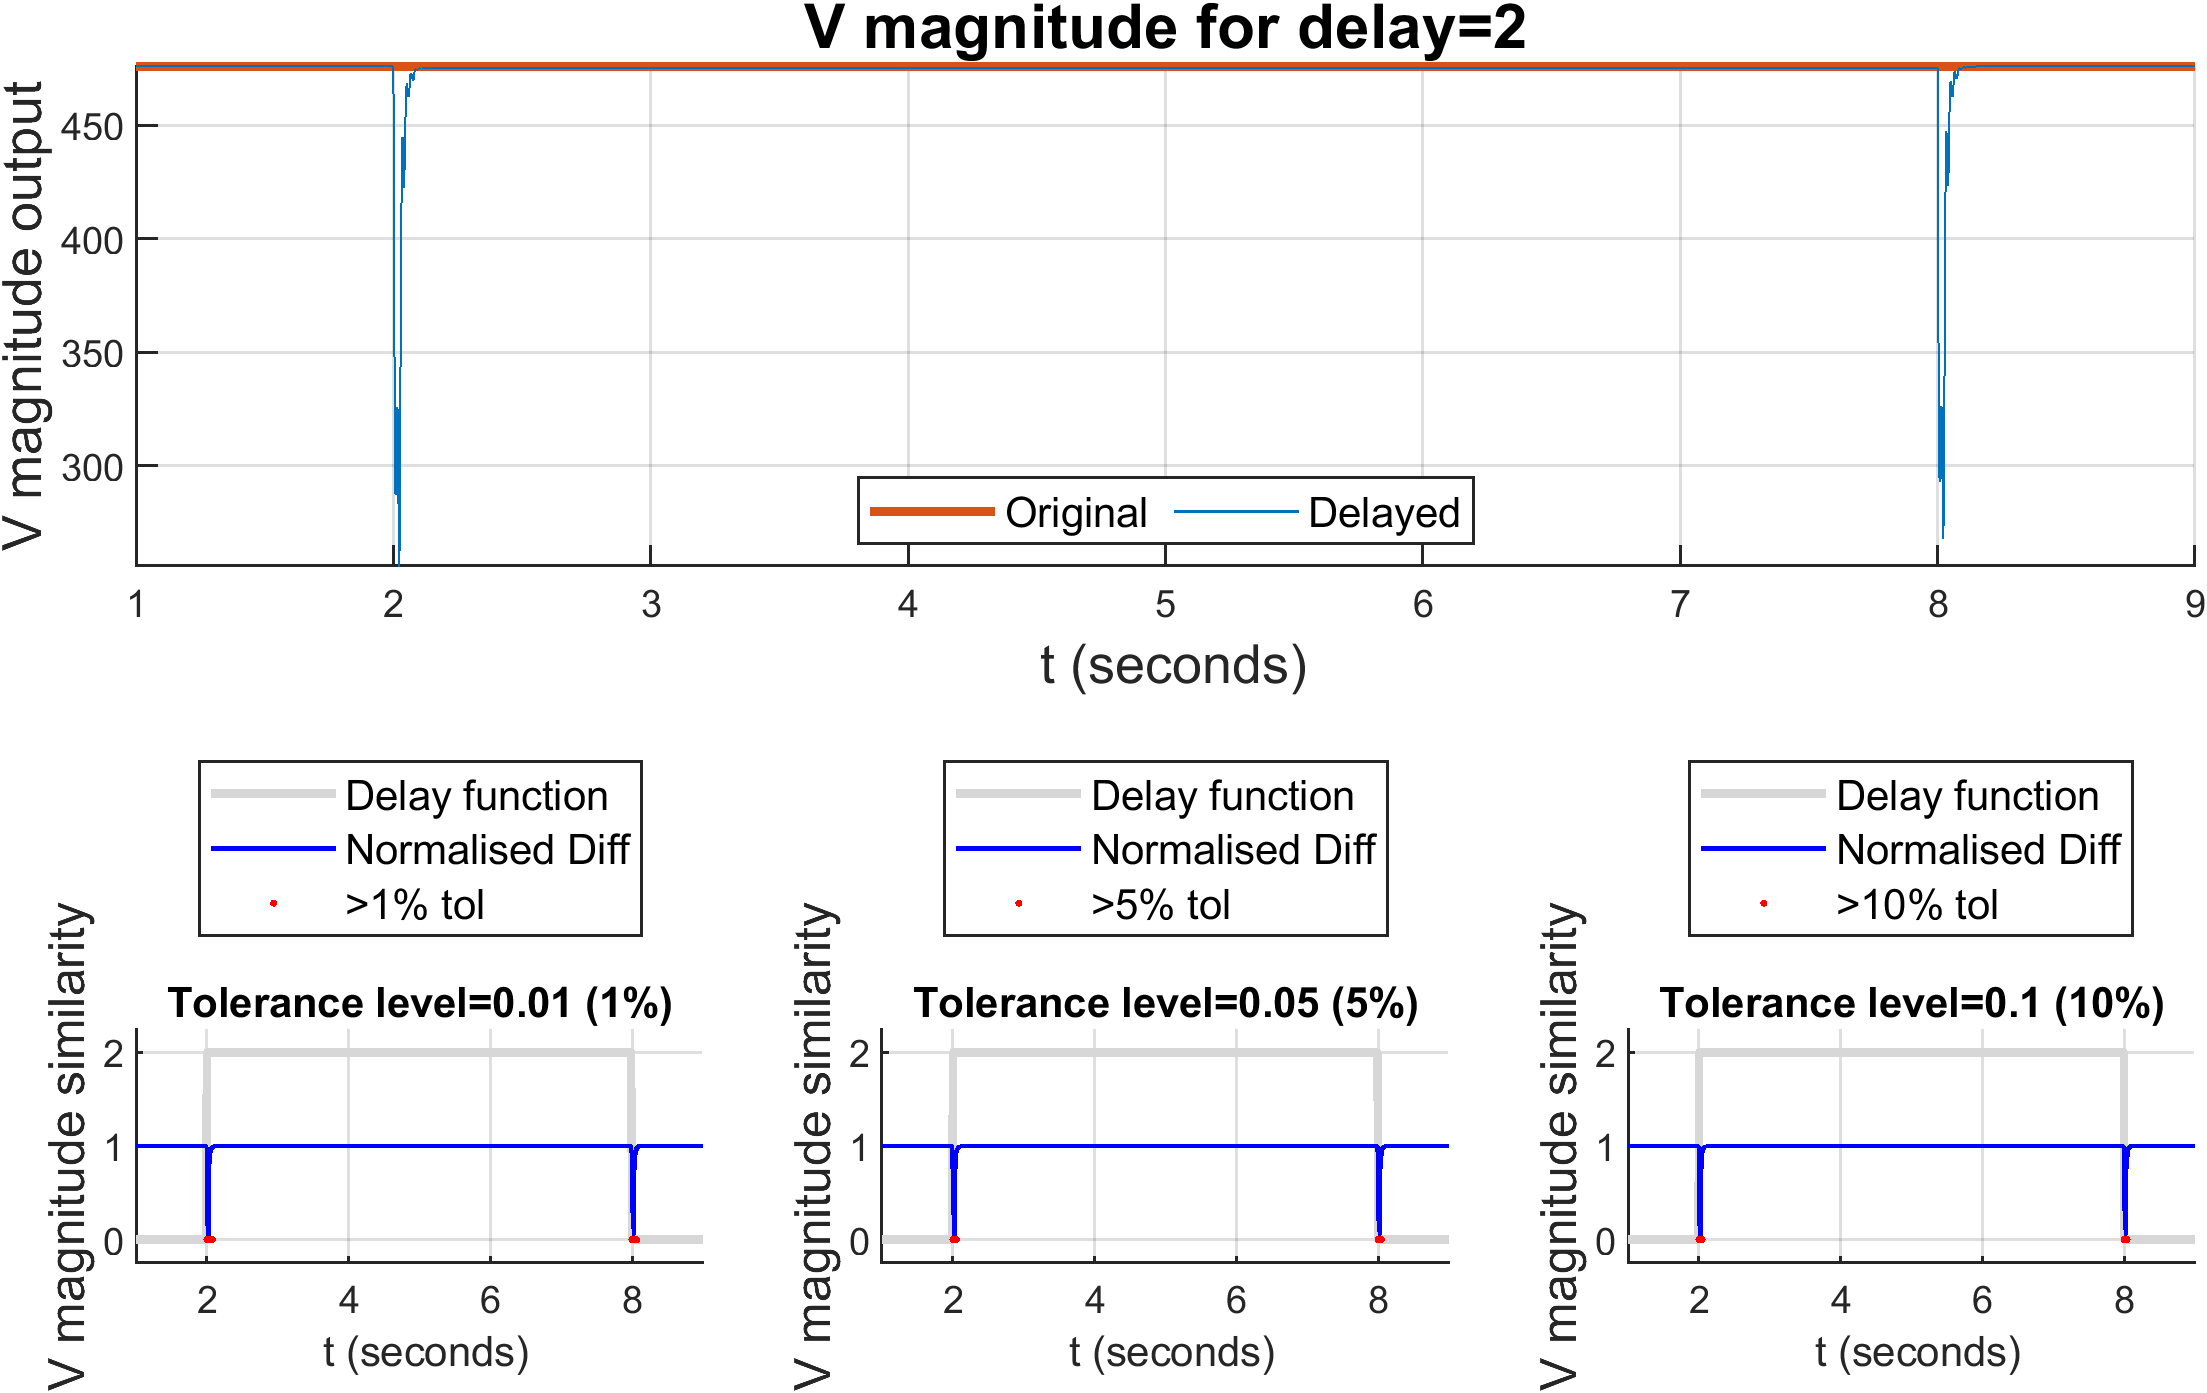
\includegraphics[width=0.95\textwidth]{PMUsim-figures/DelayOf_2/Instant_vMagnitude.png}} \\ 
    \fbox{     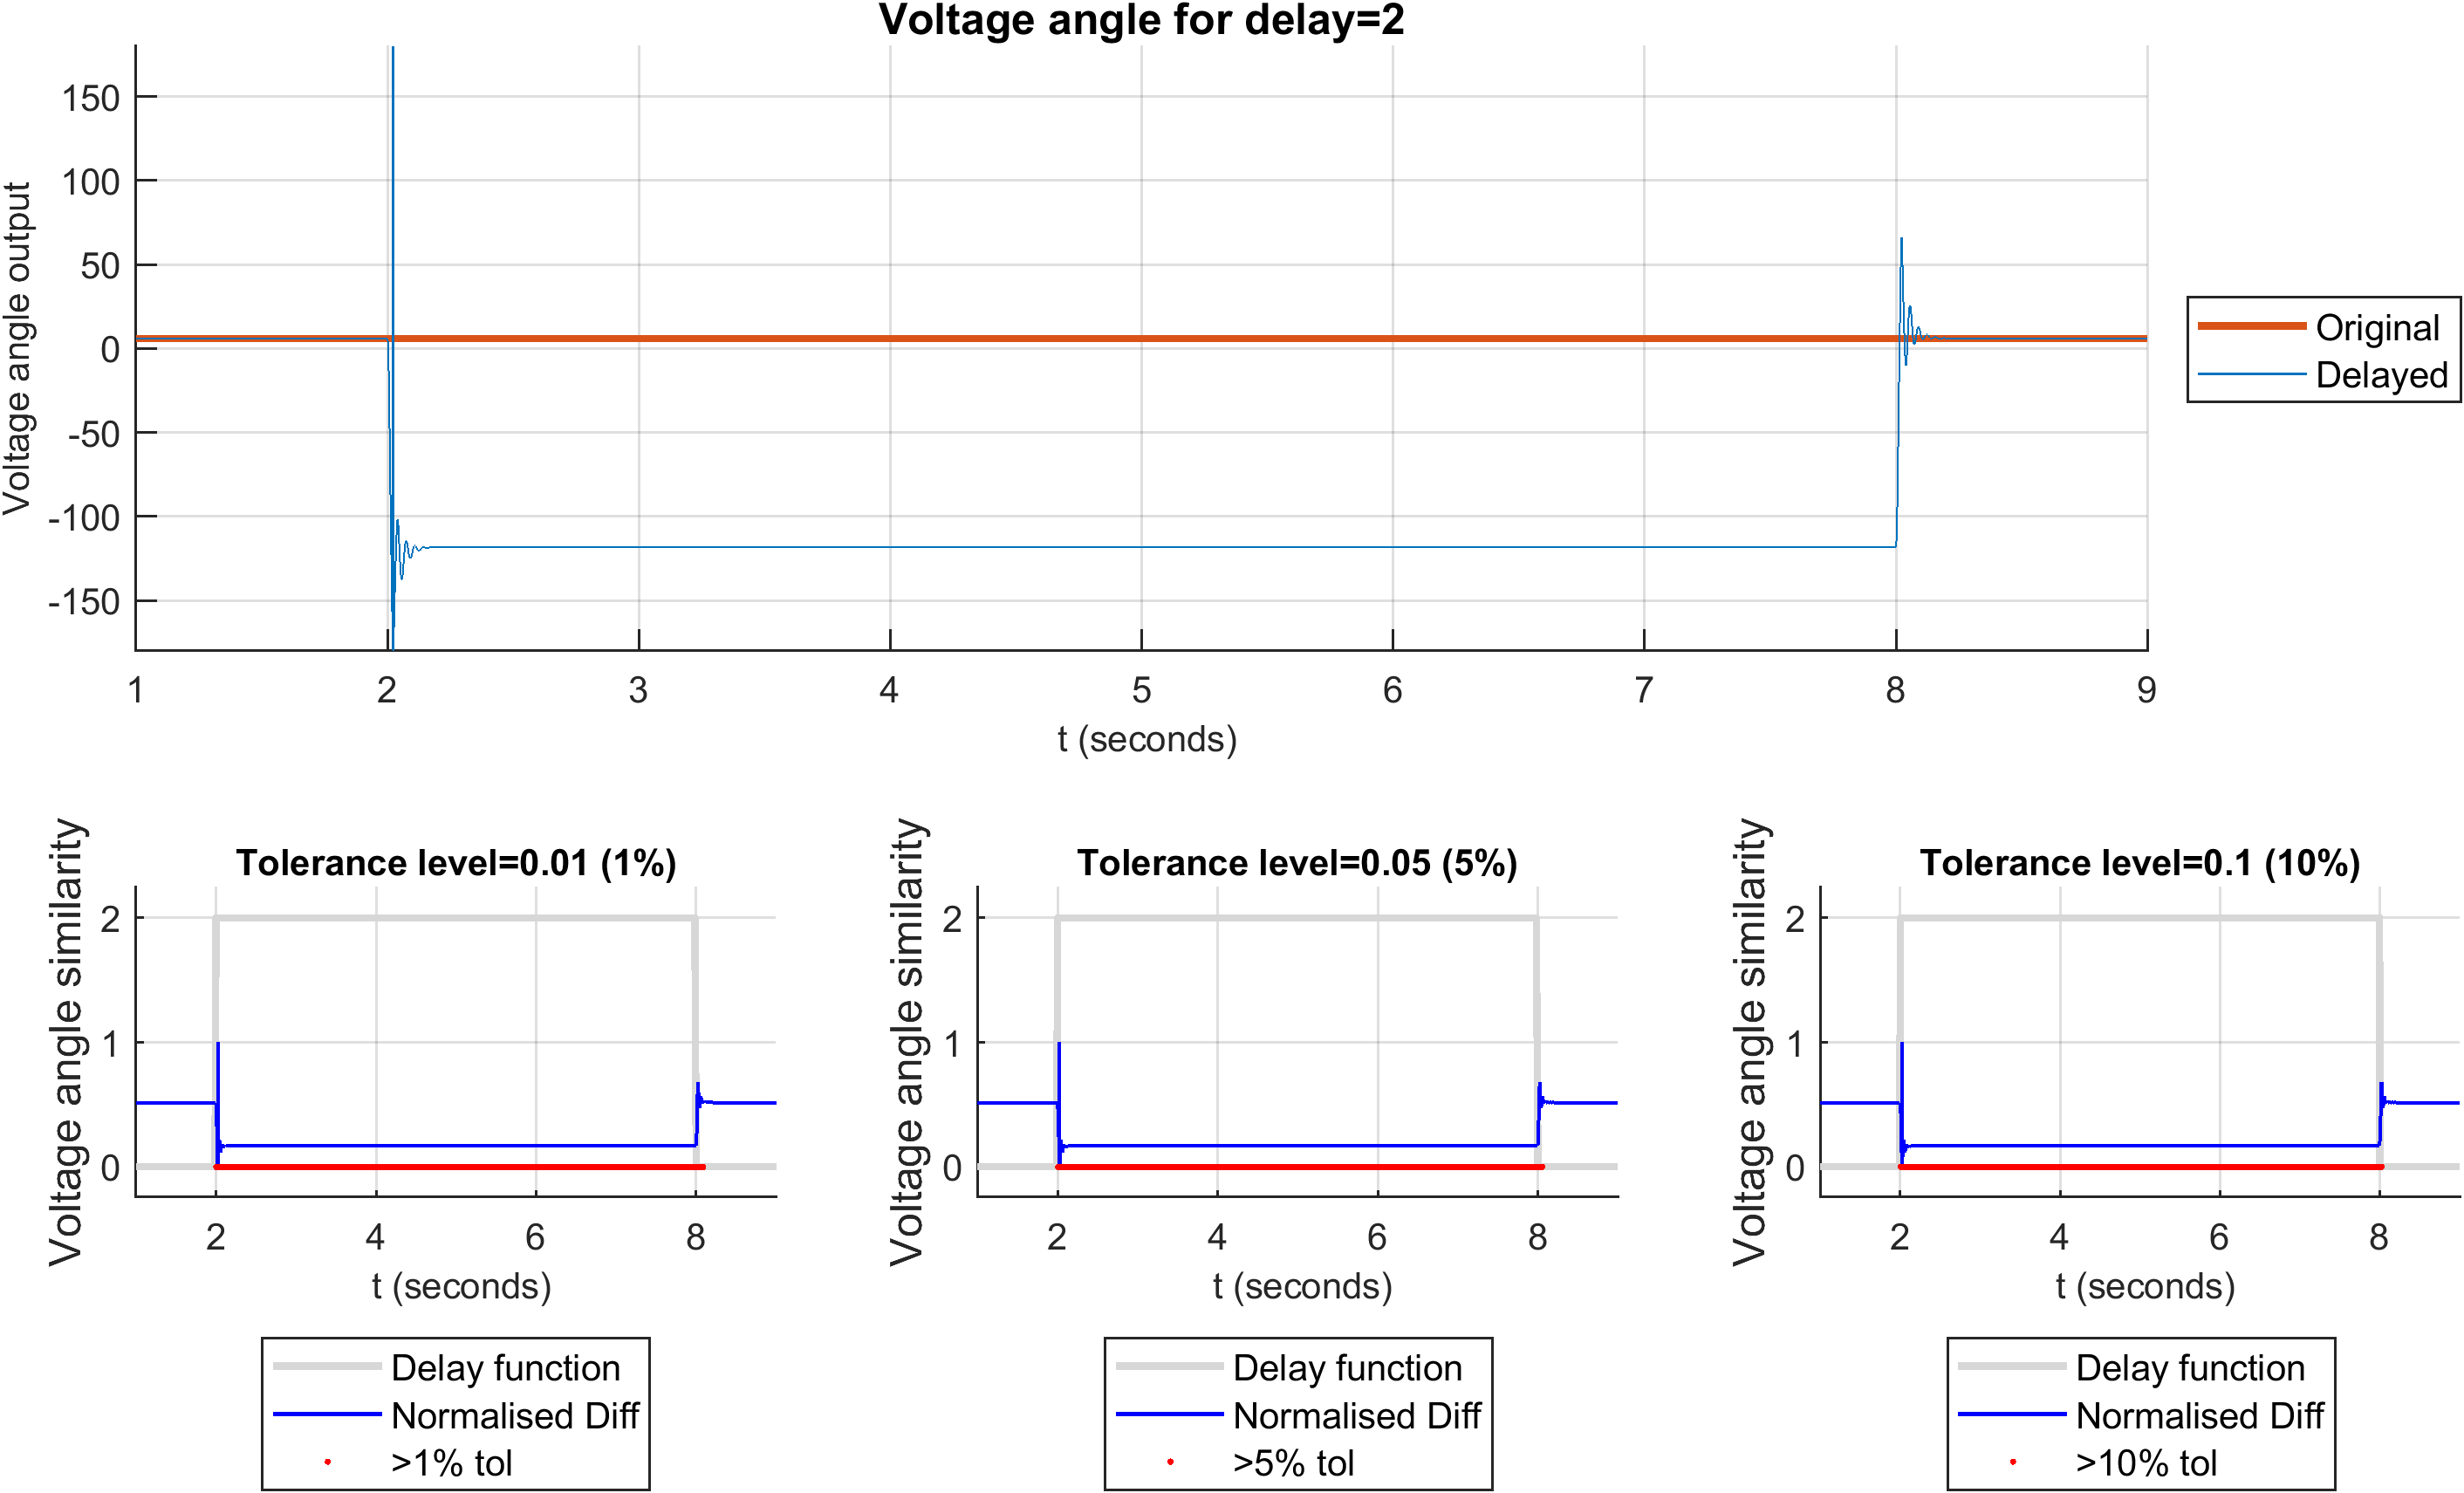
\includegraphics[width=0.95\textwidth]{PMUsim-figures/DelayOf_2/Instant_vAngle.png}} \\  
   \fbox{    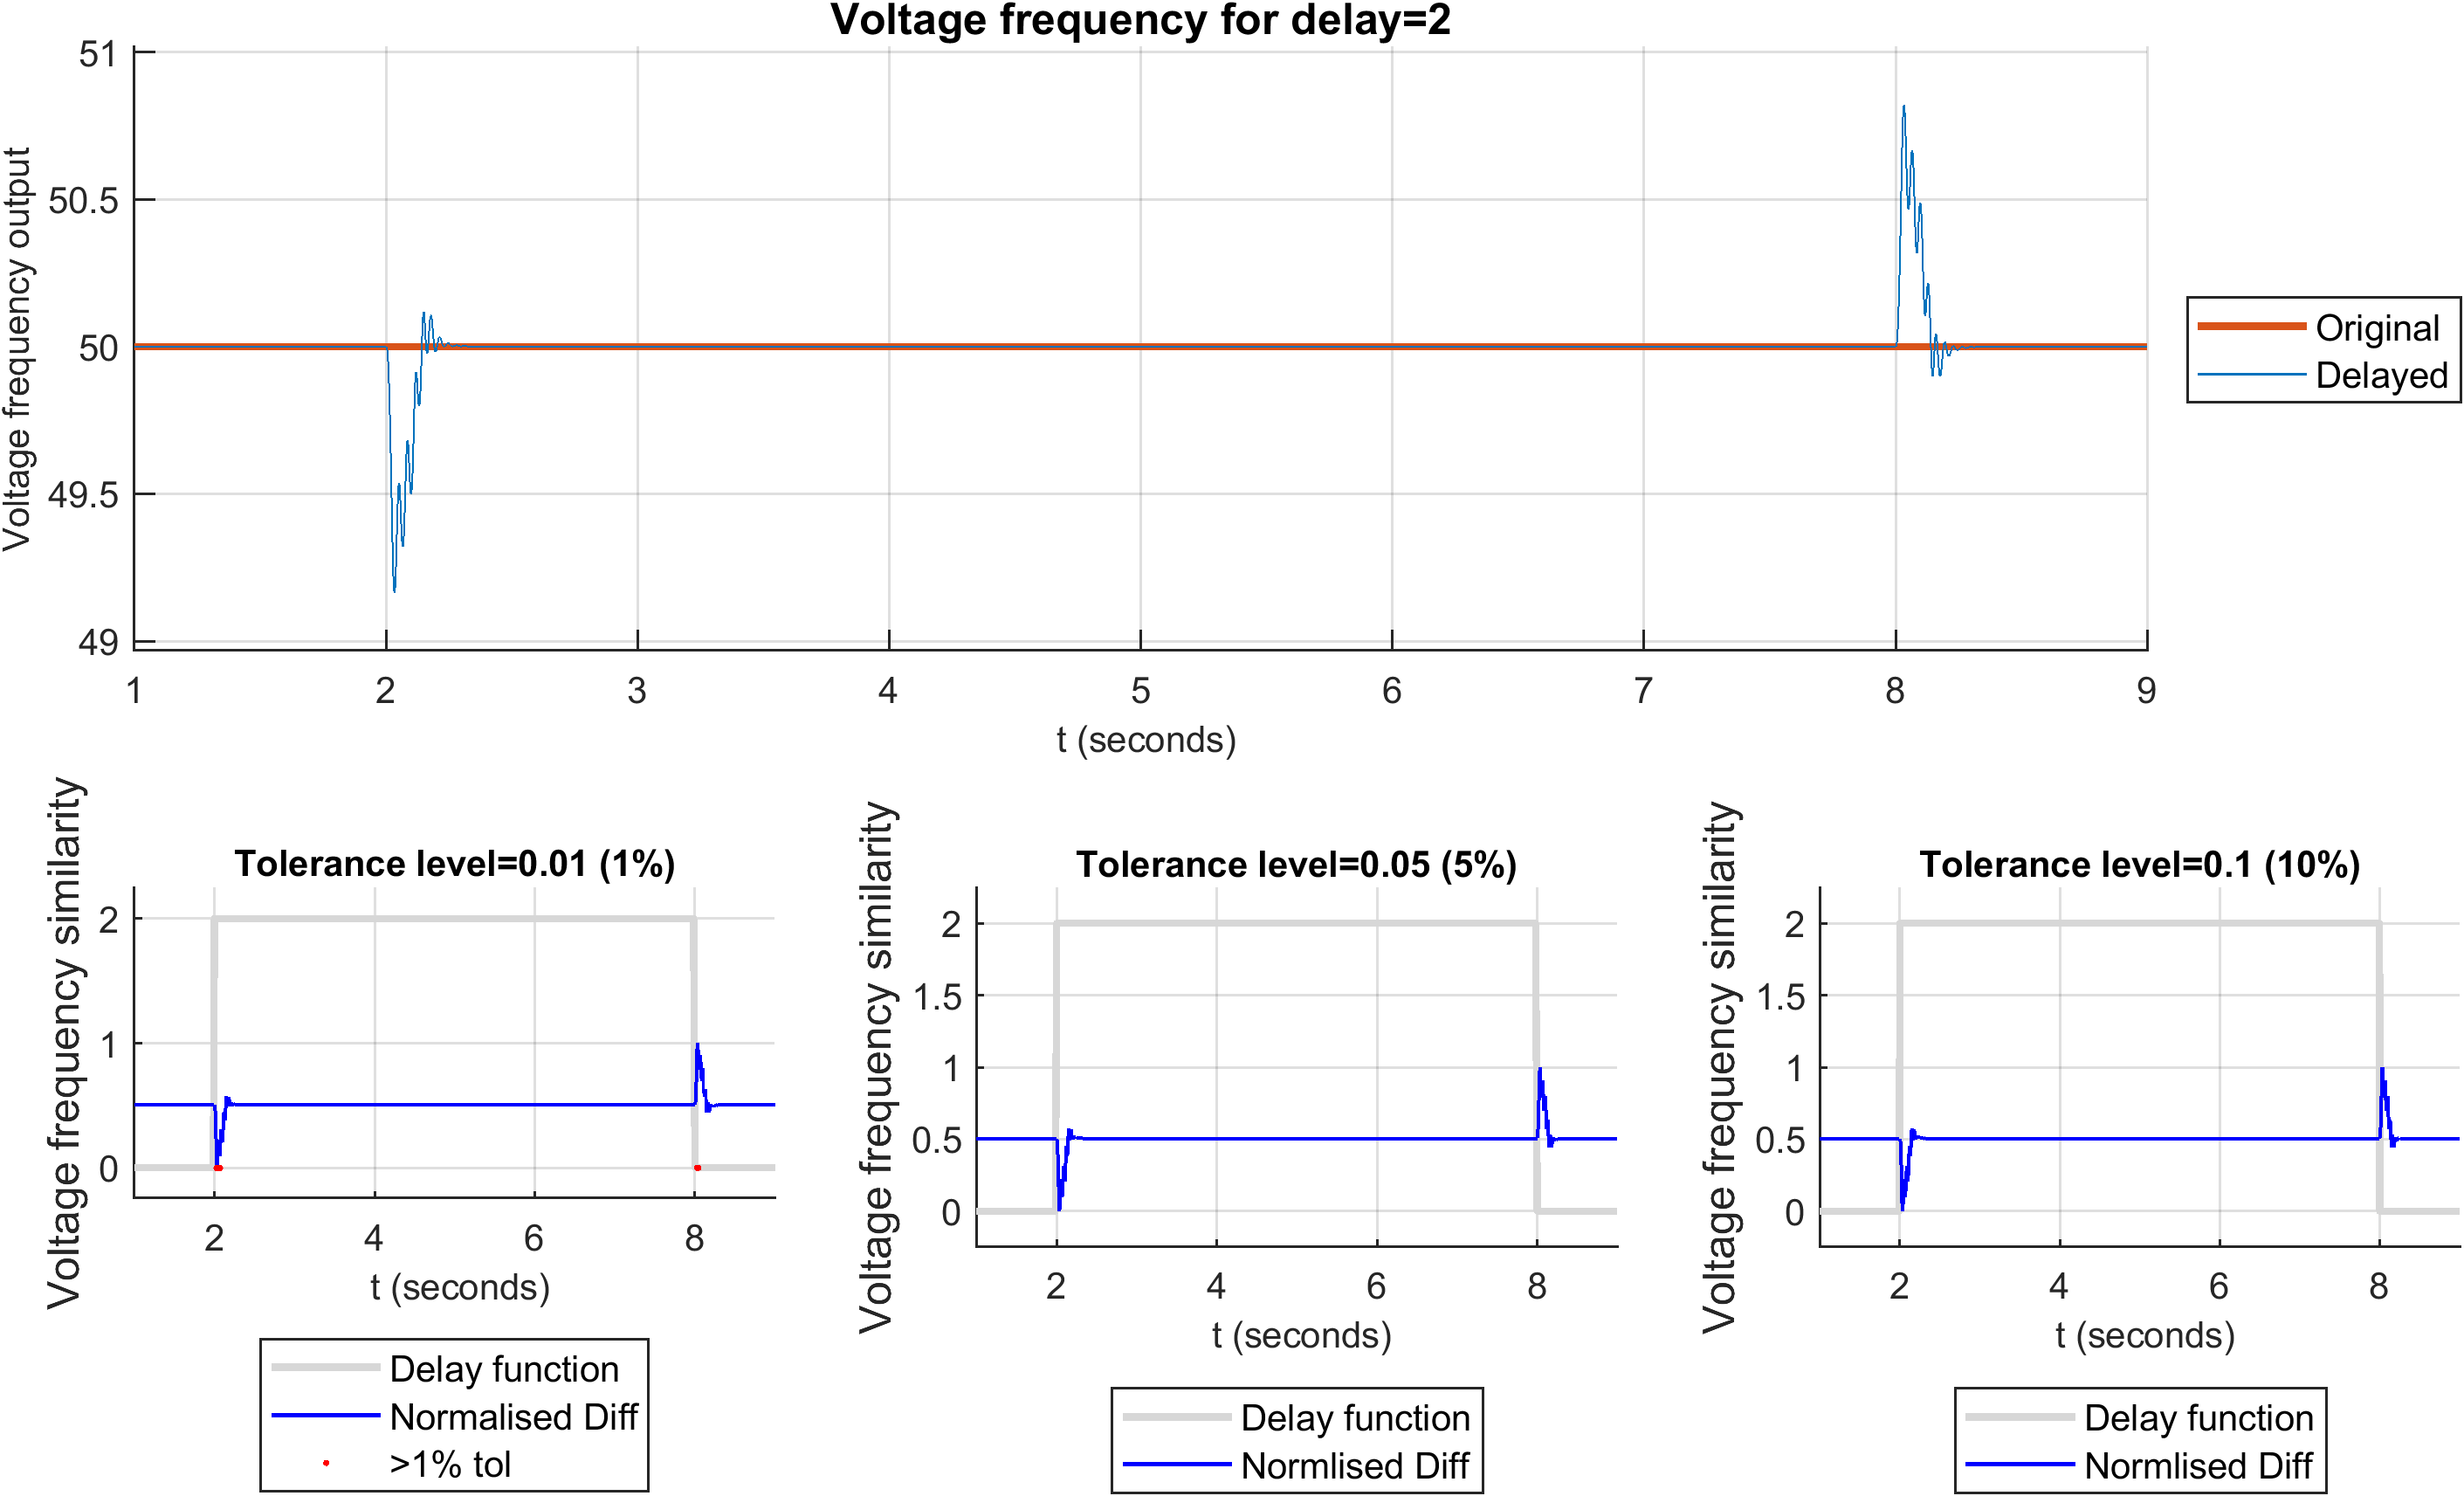
\includegraphics[width=0.95\textwidth]{PMUsim-figures/DelayOf_2/Instant_vFrequency.png}}

 
  \end{tabular}
\label{fig:VoltageInstantDelayTwo}
\caption{Results for Voltage Output for Instant Delay equal to Two }
\end{figure}

\newpage
\begin{figure}[H]
\begin{tabular}{c}
  \fbox{  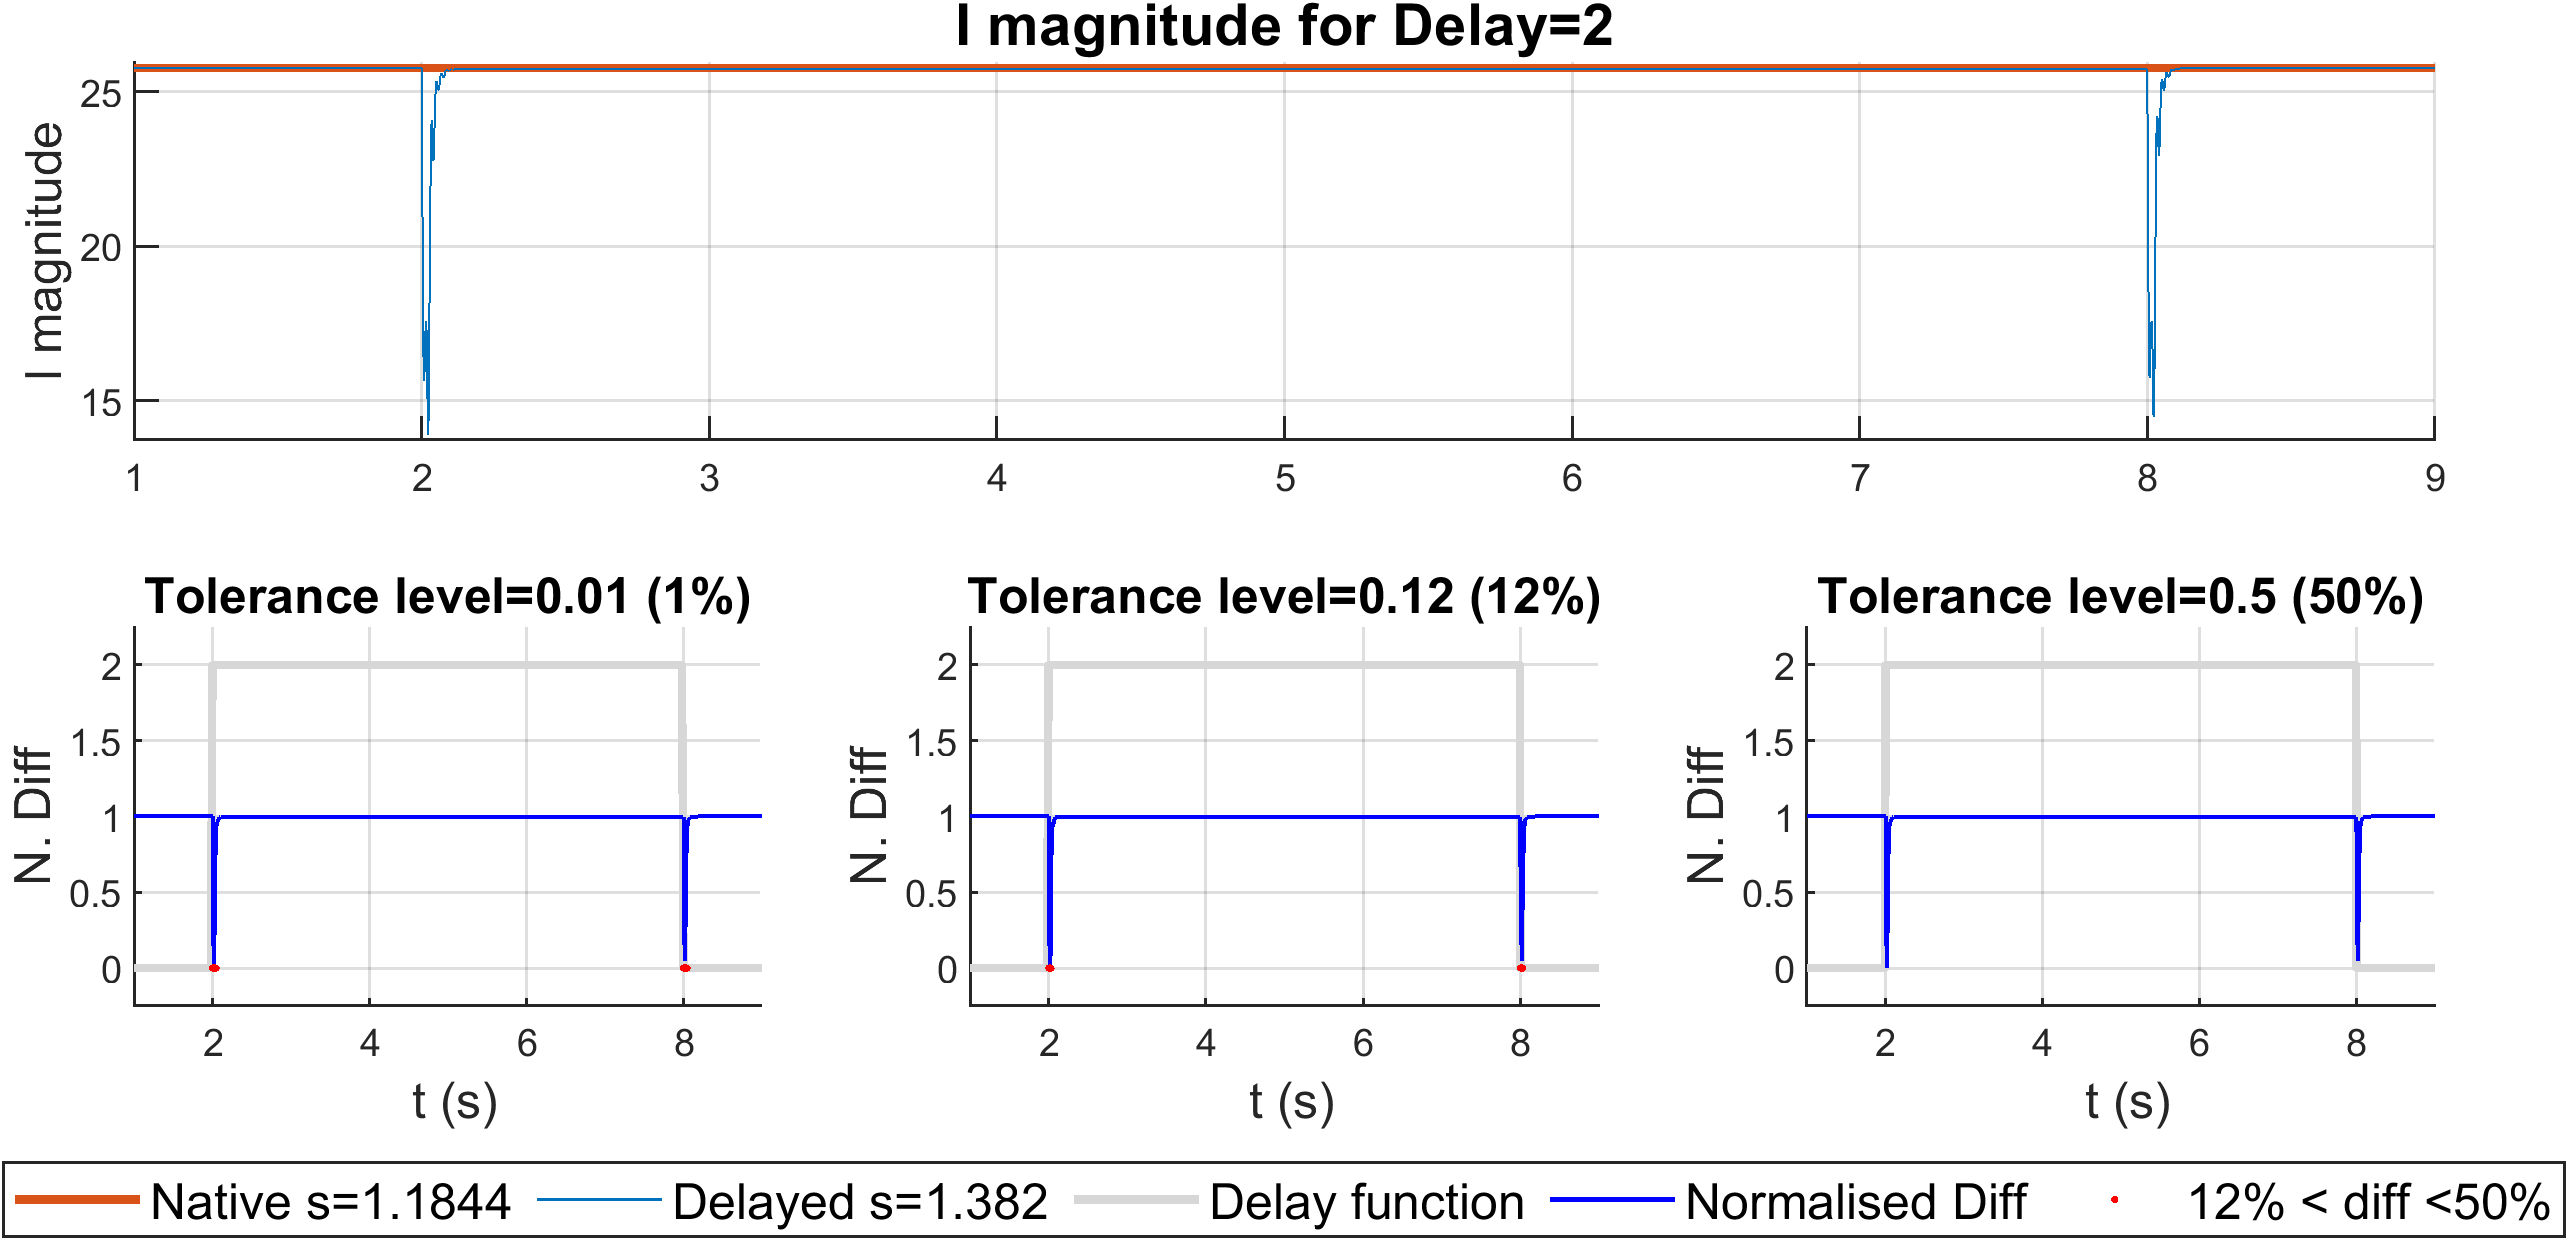
\includegraphics[width=0.95\textwidth]{PMUsim-figures/DelayOf_2/Instant_iMagnitude.png}} \\ 
    \fbox{     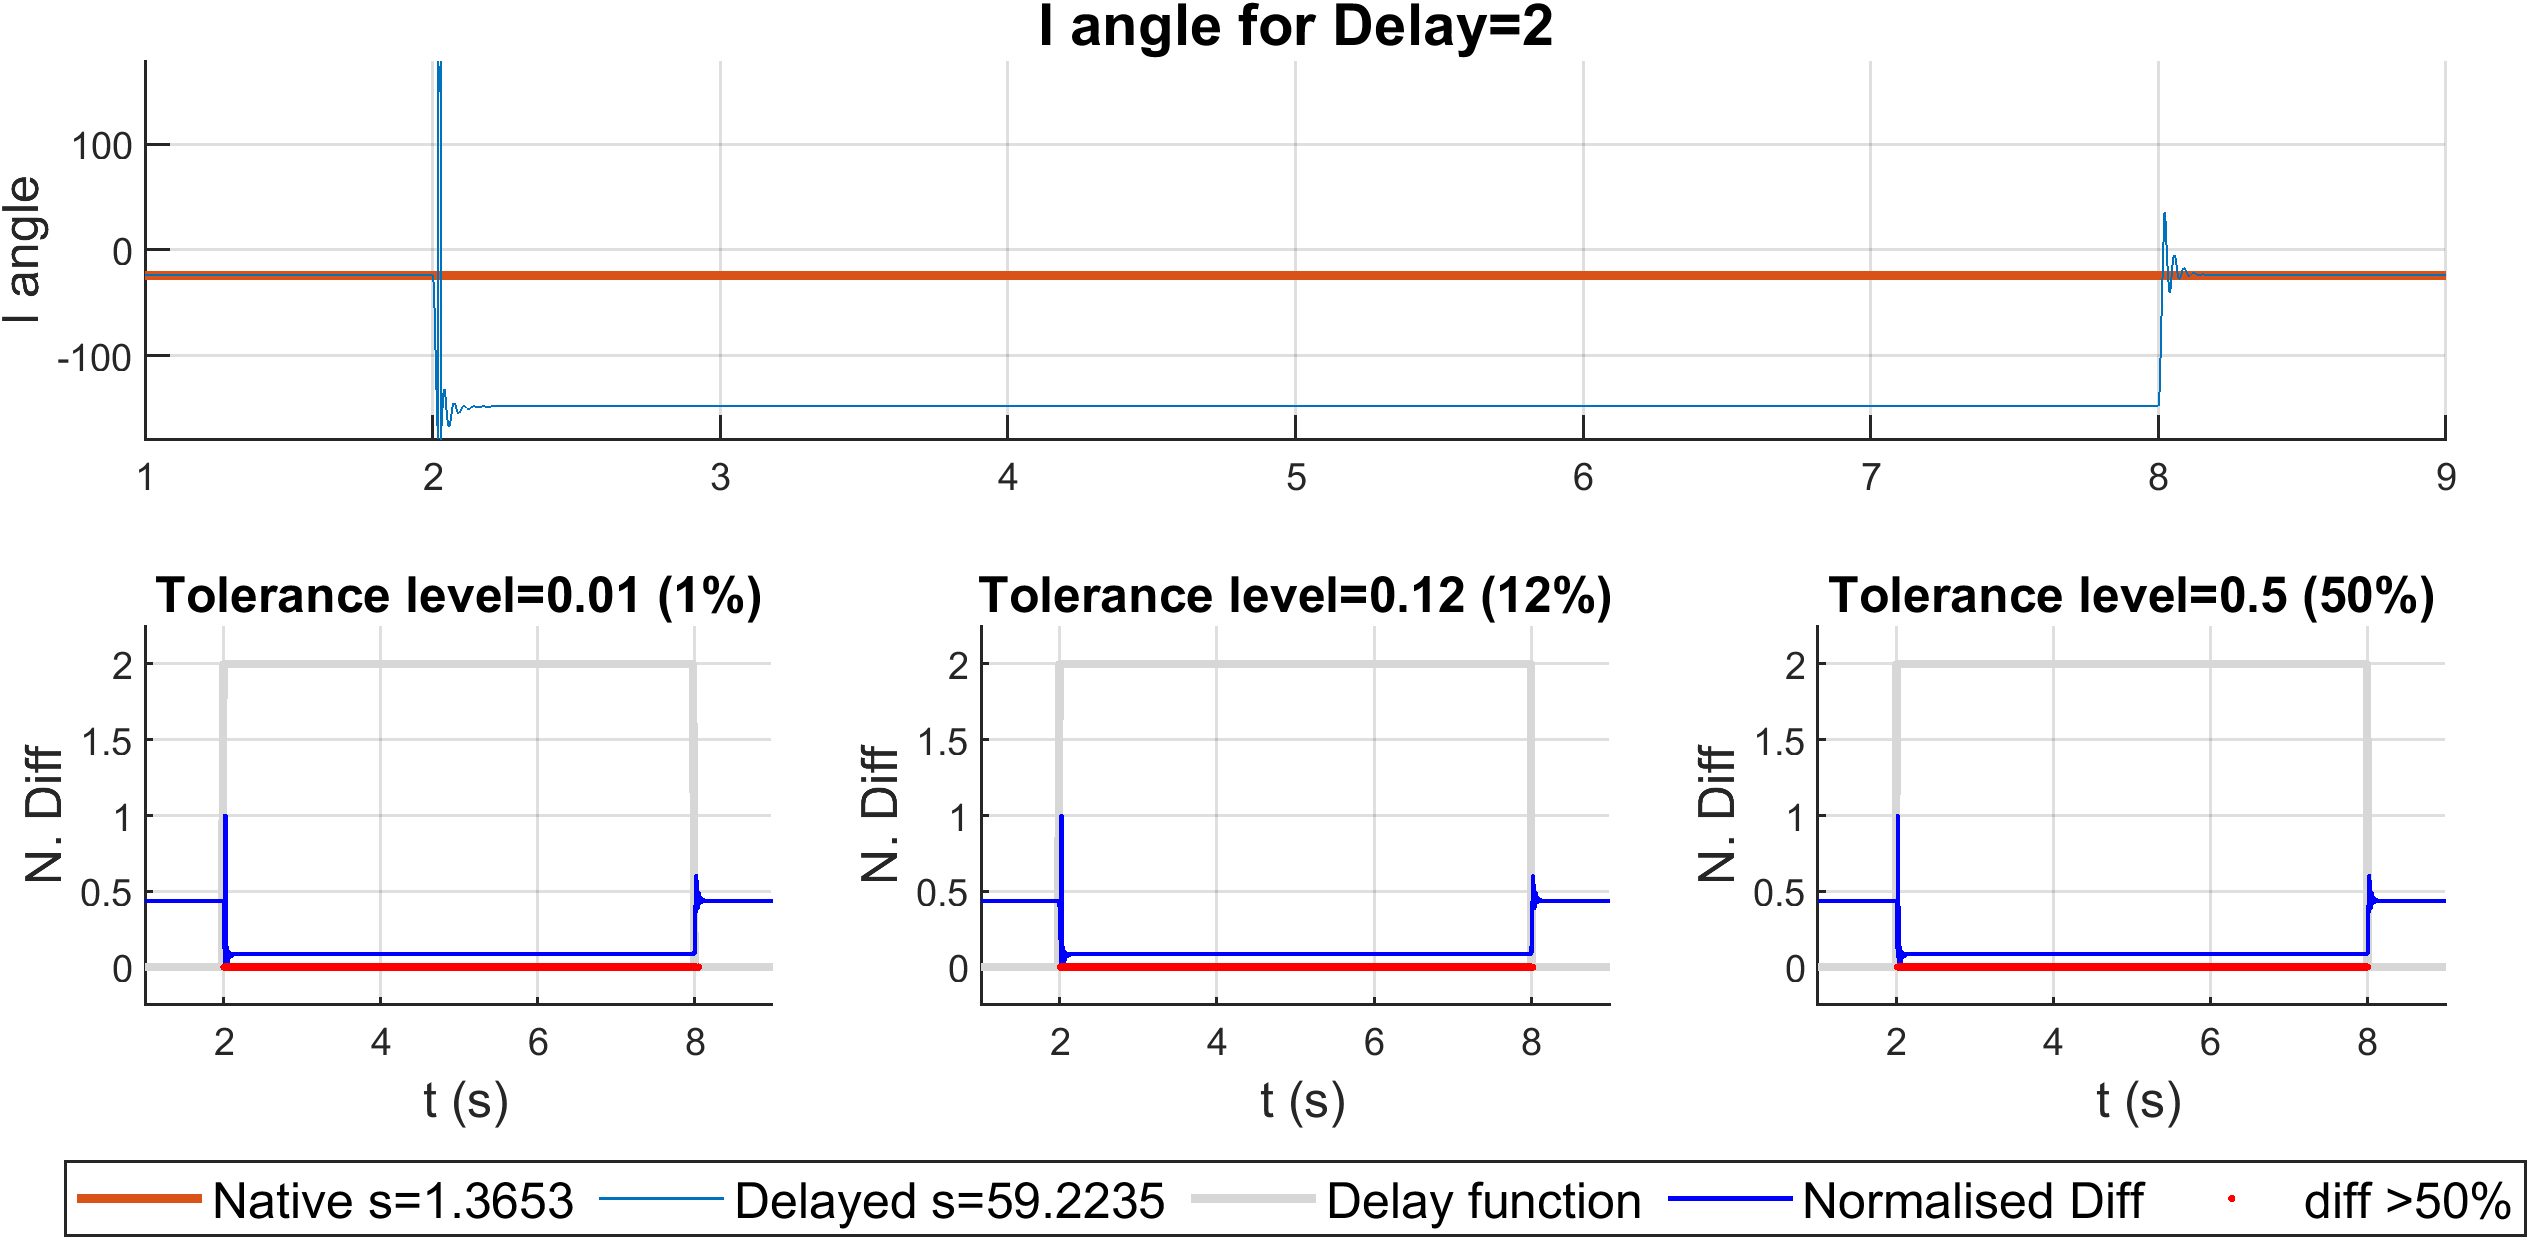
\includegraphics[width=0.95\textwidth]{PMUsim-figures/DelayOf_2/Instant_iAngle.png}} \\   
   \fbox{    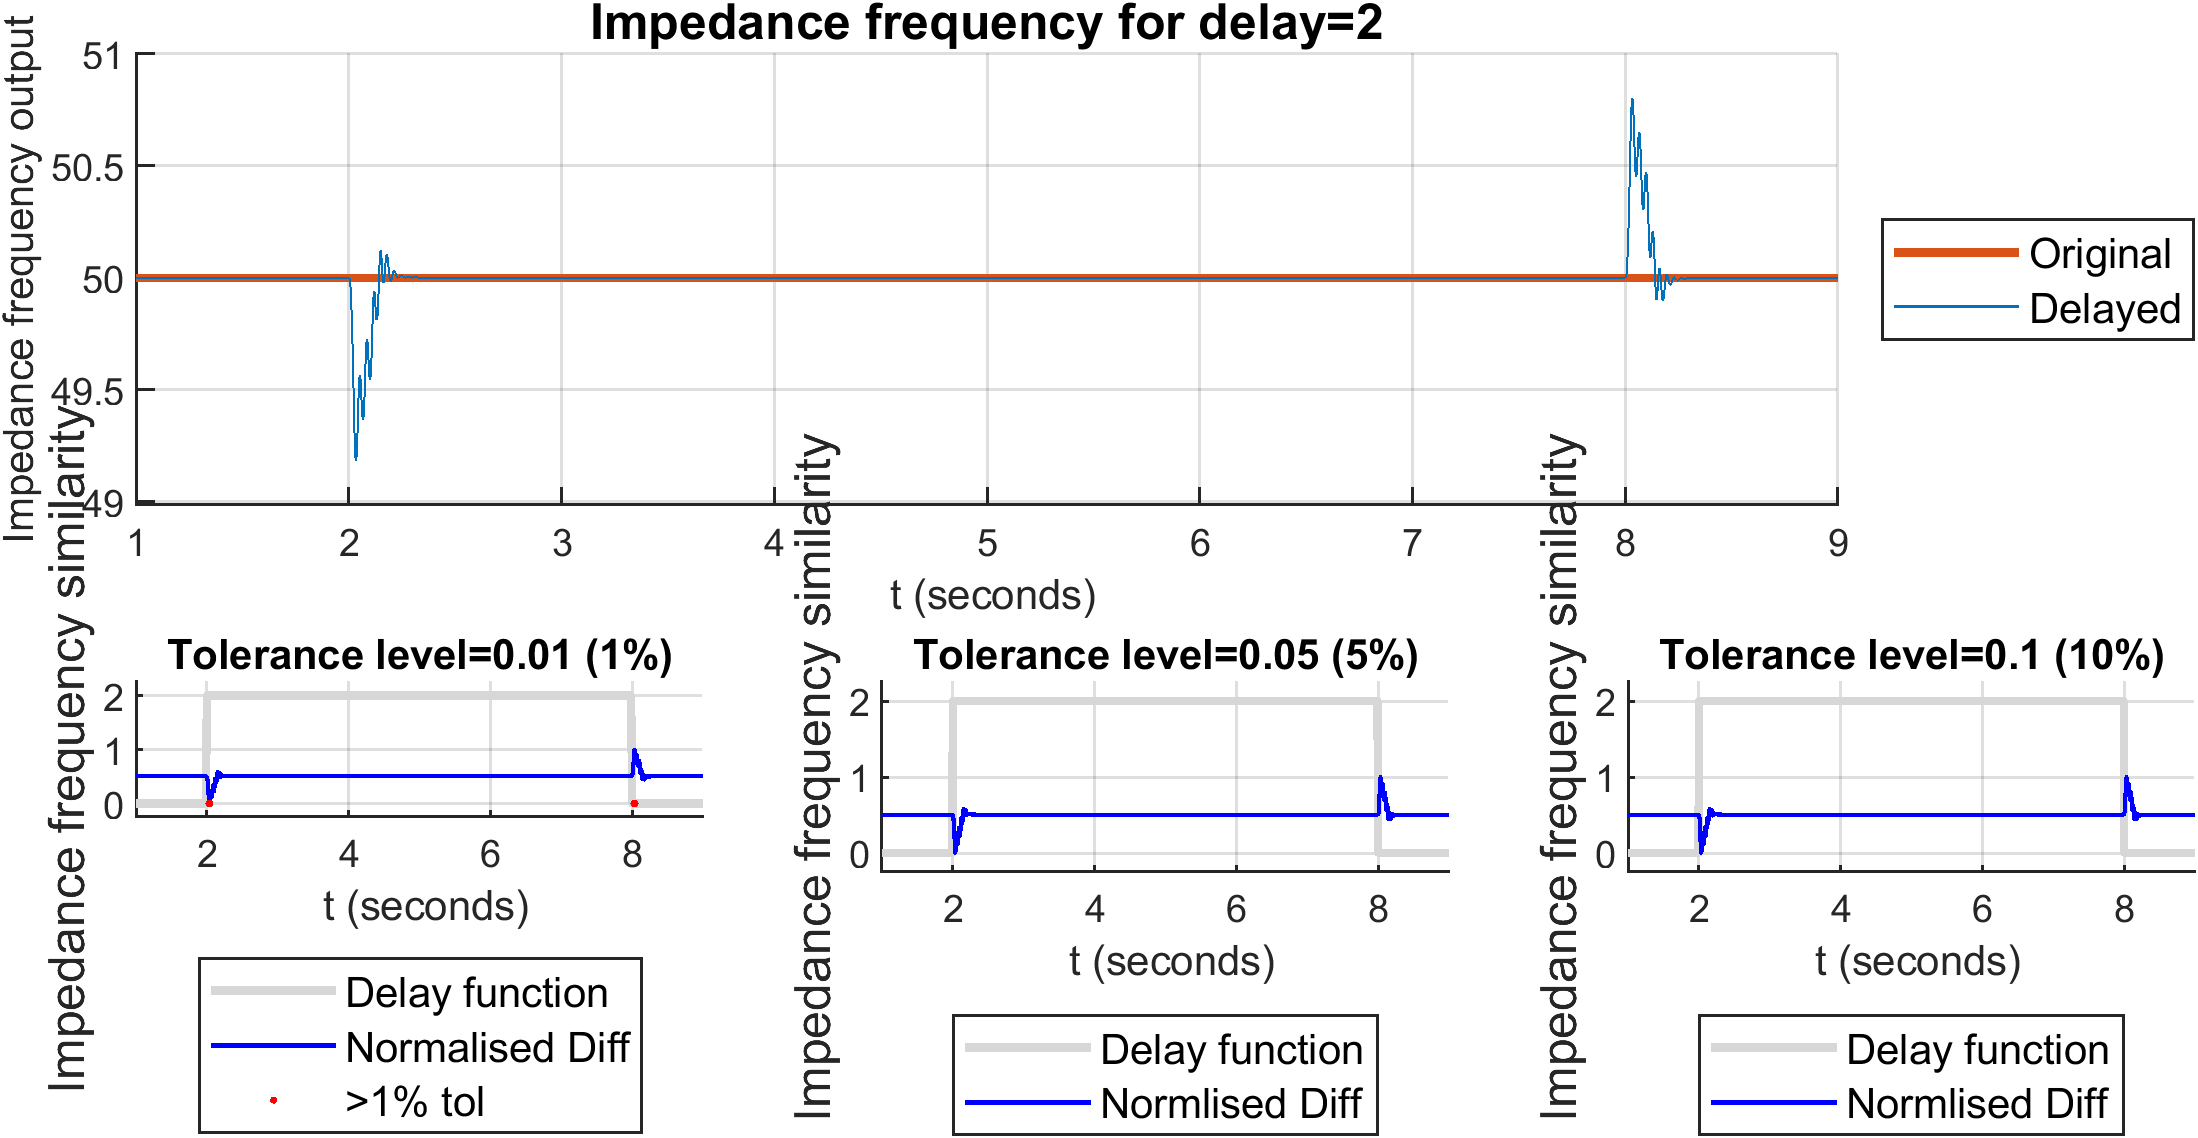
\includegraphics[width=0.95\textwidth]{PMUsim-figures/DelayOf_2/Instant_iFrequency.png}}


  \end{tabular}
\label{fig:ImpedanceInstantDelayTwo}
\caption{Results for Impedance Output for Instant Delay equal to Two }
\end{figure}





\newpage
\begin{figure}[H]
\begin{tabular}{c}
  \fbox{  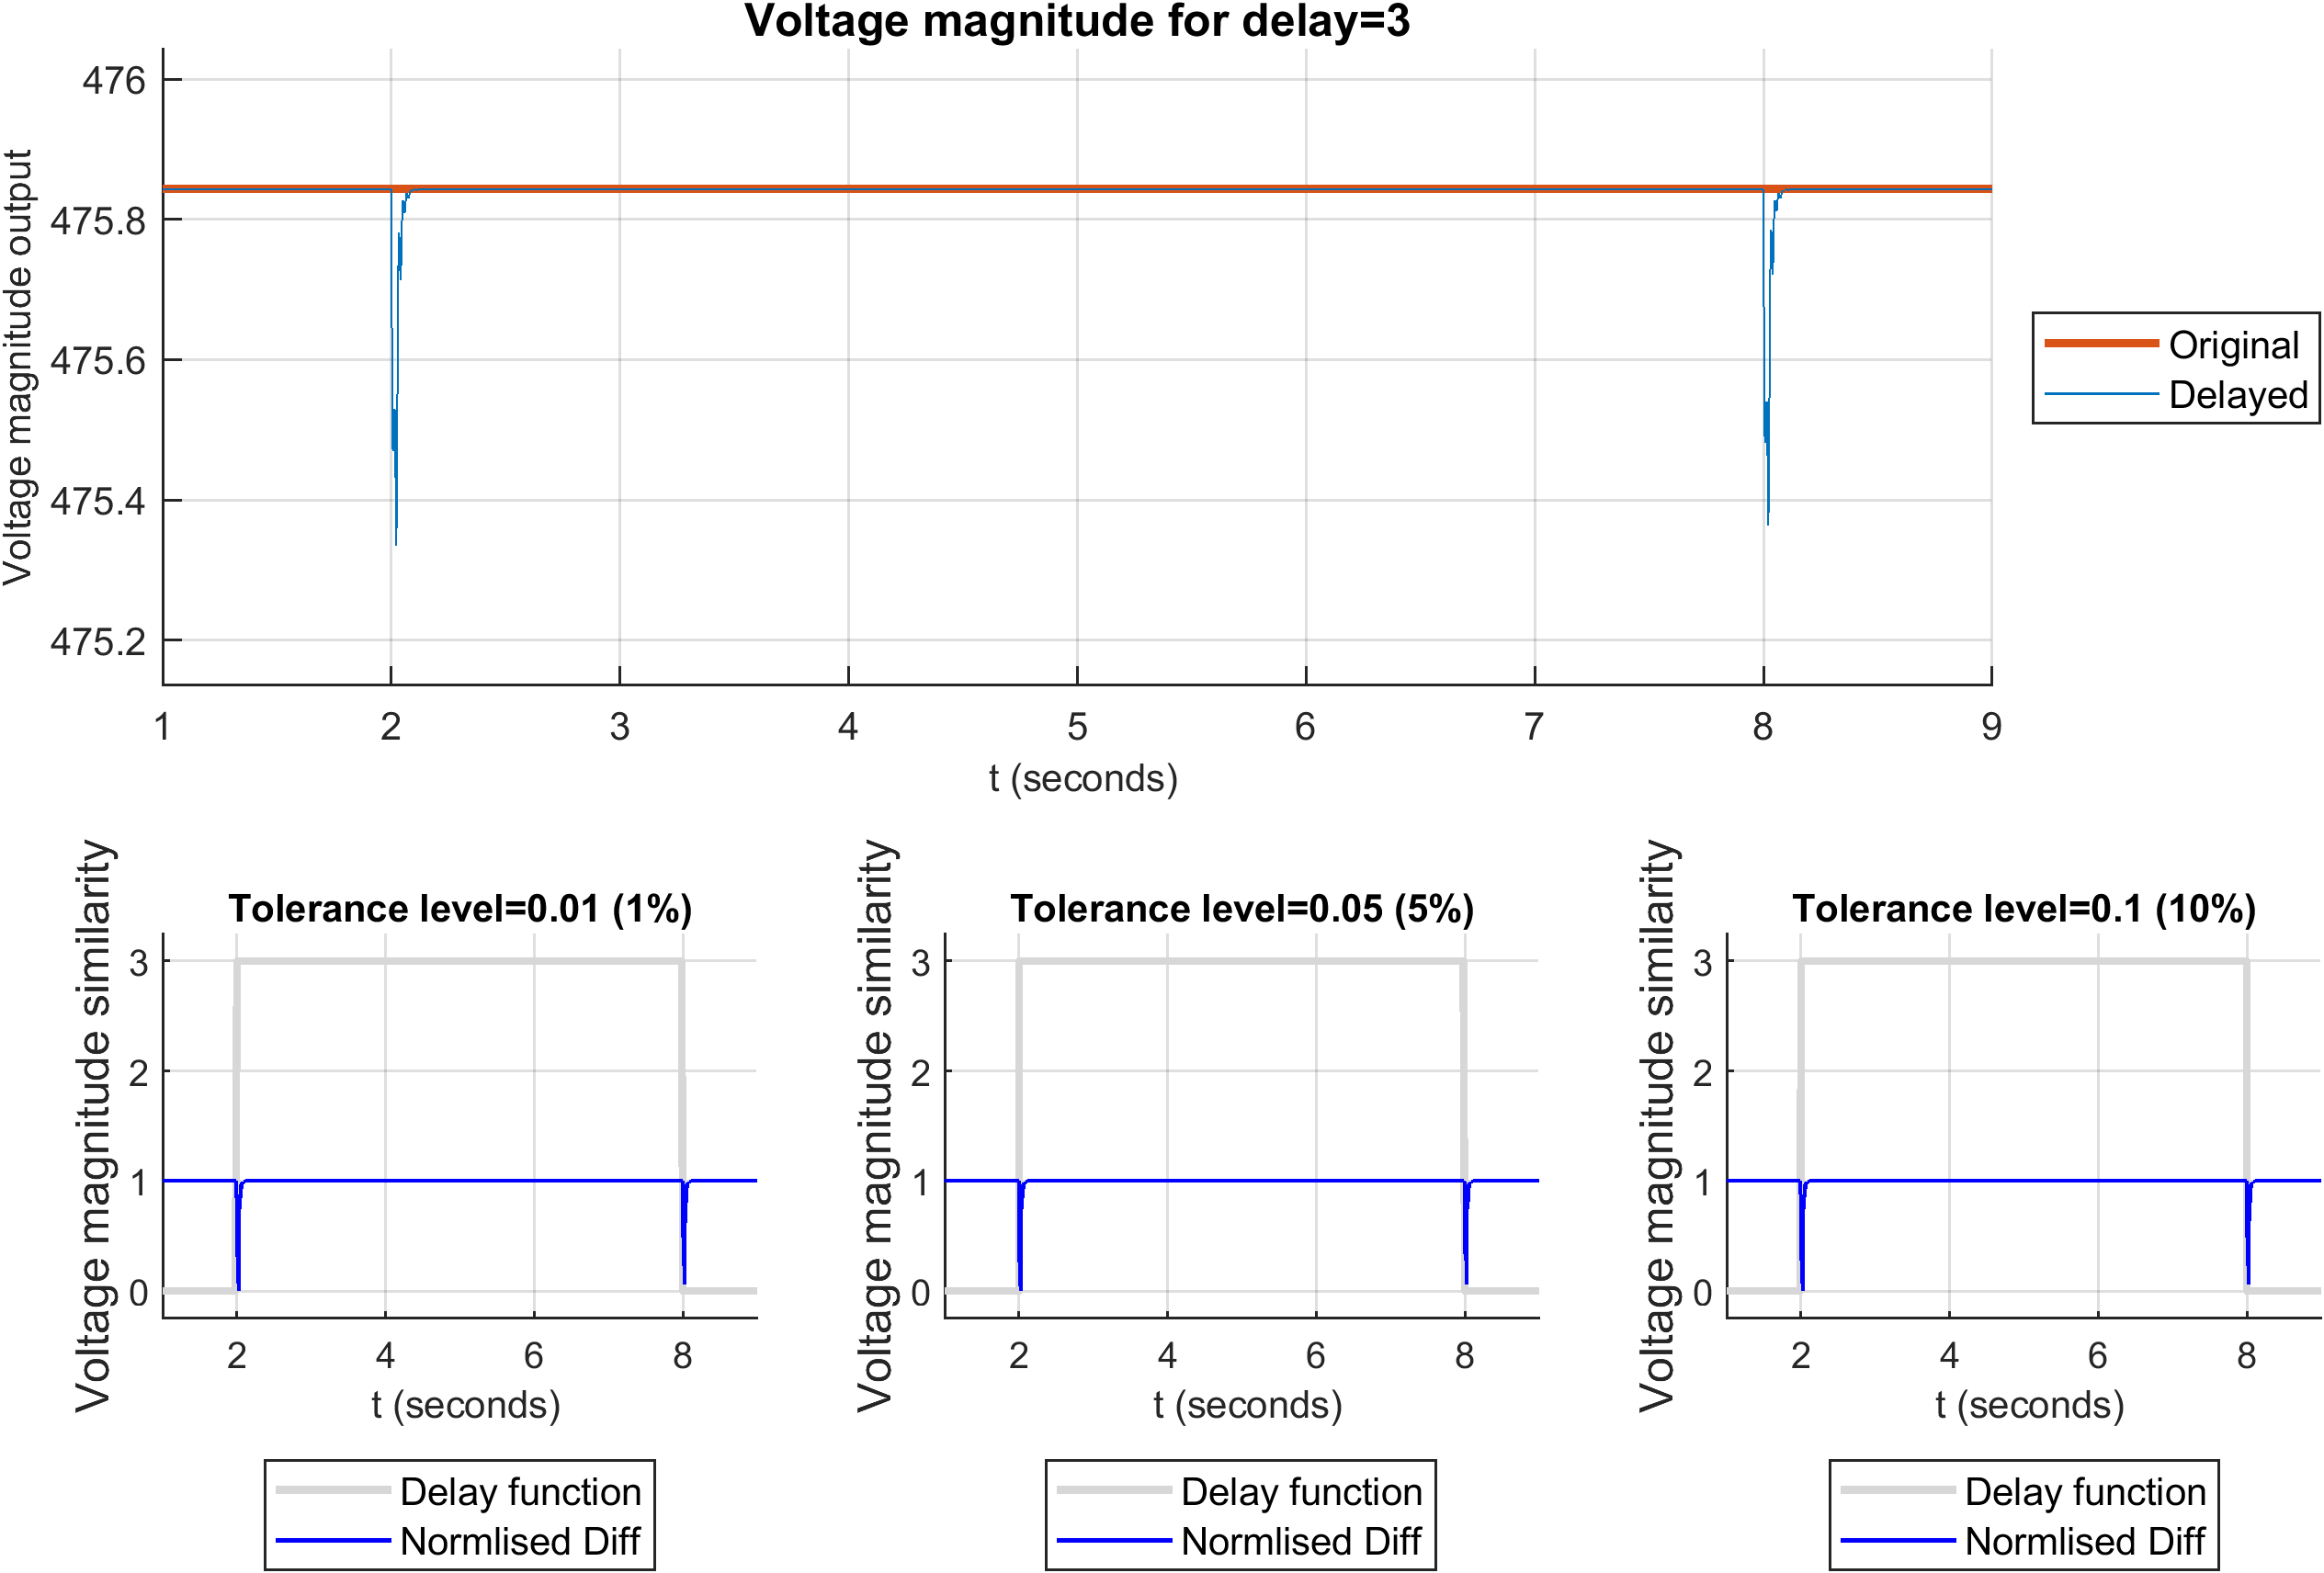
\includegraphics[width=0.95\textwidth]{PMUsim-figures/DelayOf_3/Instant_vMagnitude.png}} \\ 
   \fbox{     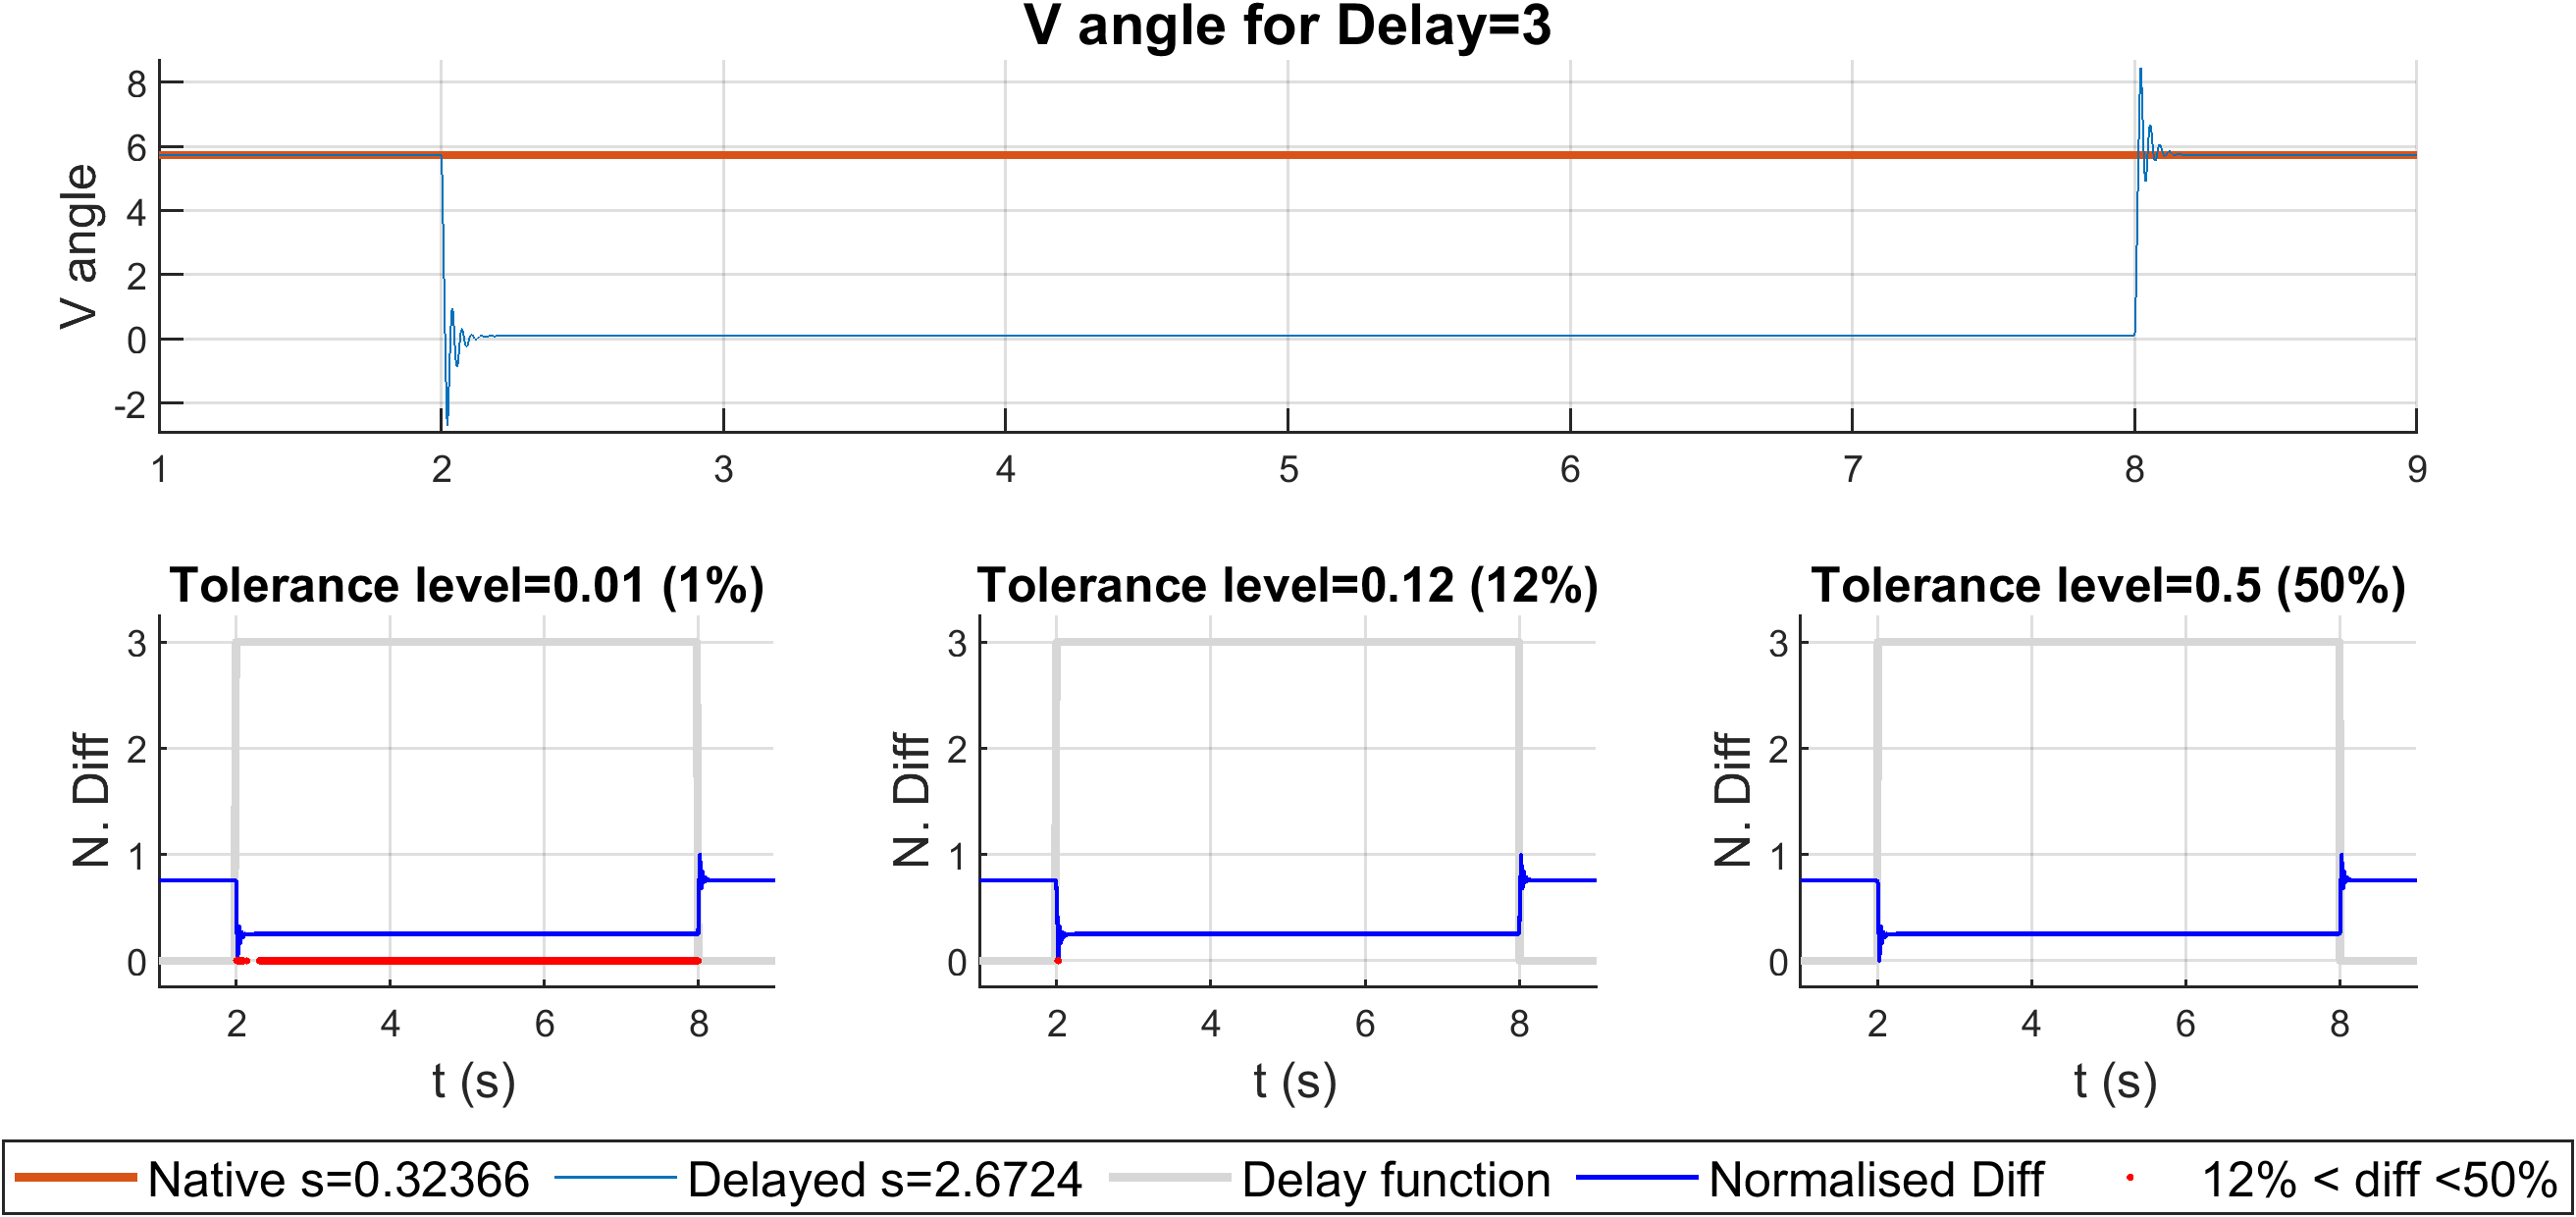
\includegraphics[width=0.95\textwidth]{PMUsim-figures/DelayOf_3/Instant_vAngle.png}} \\    
   \fbox{    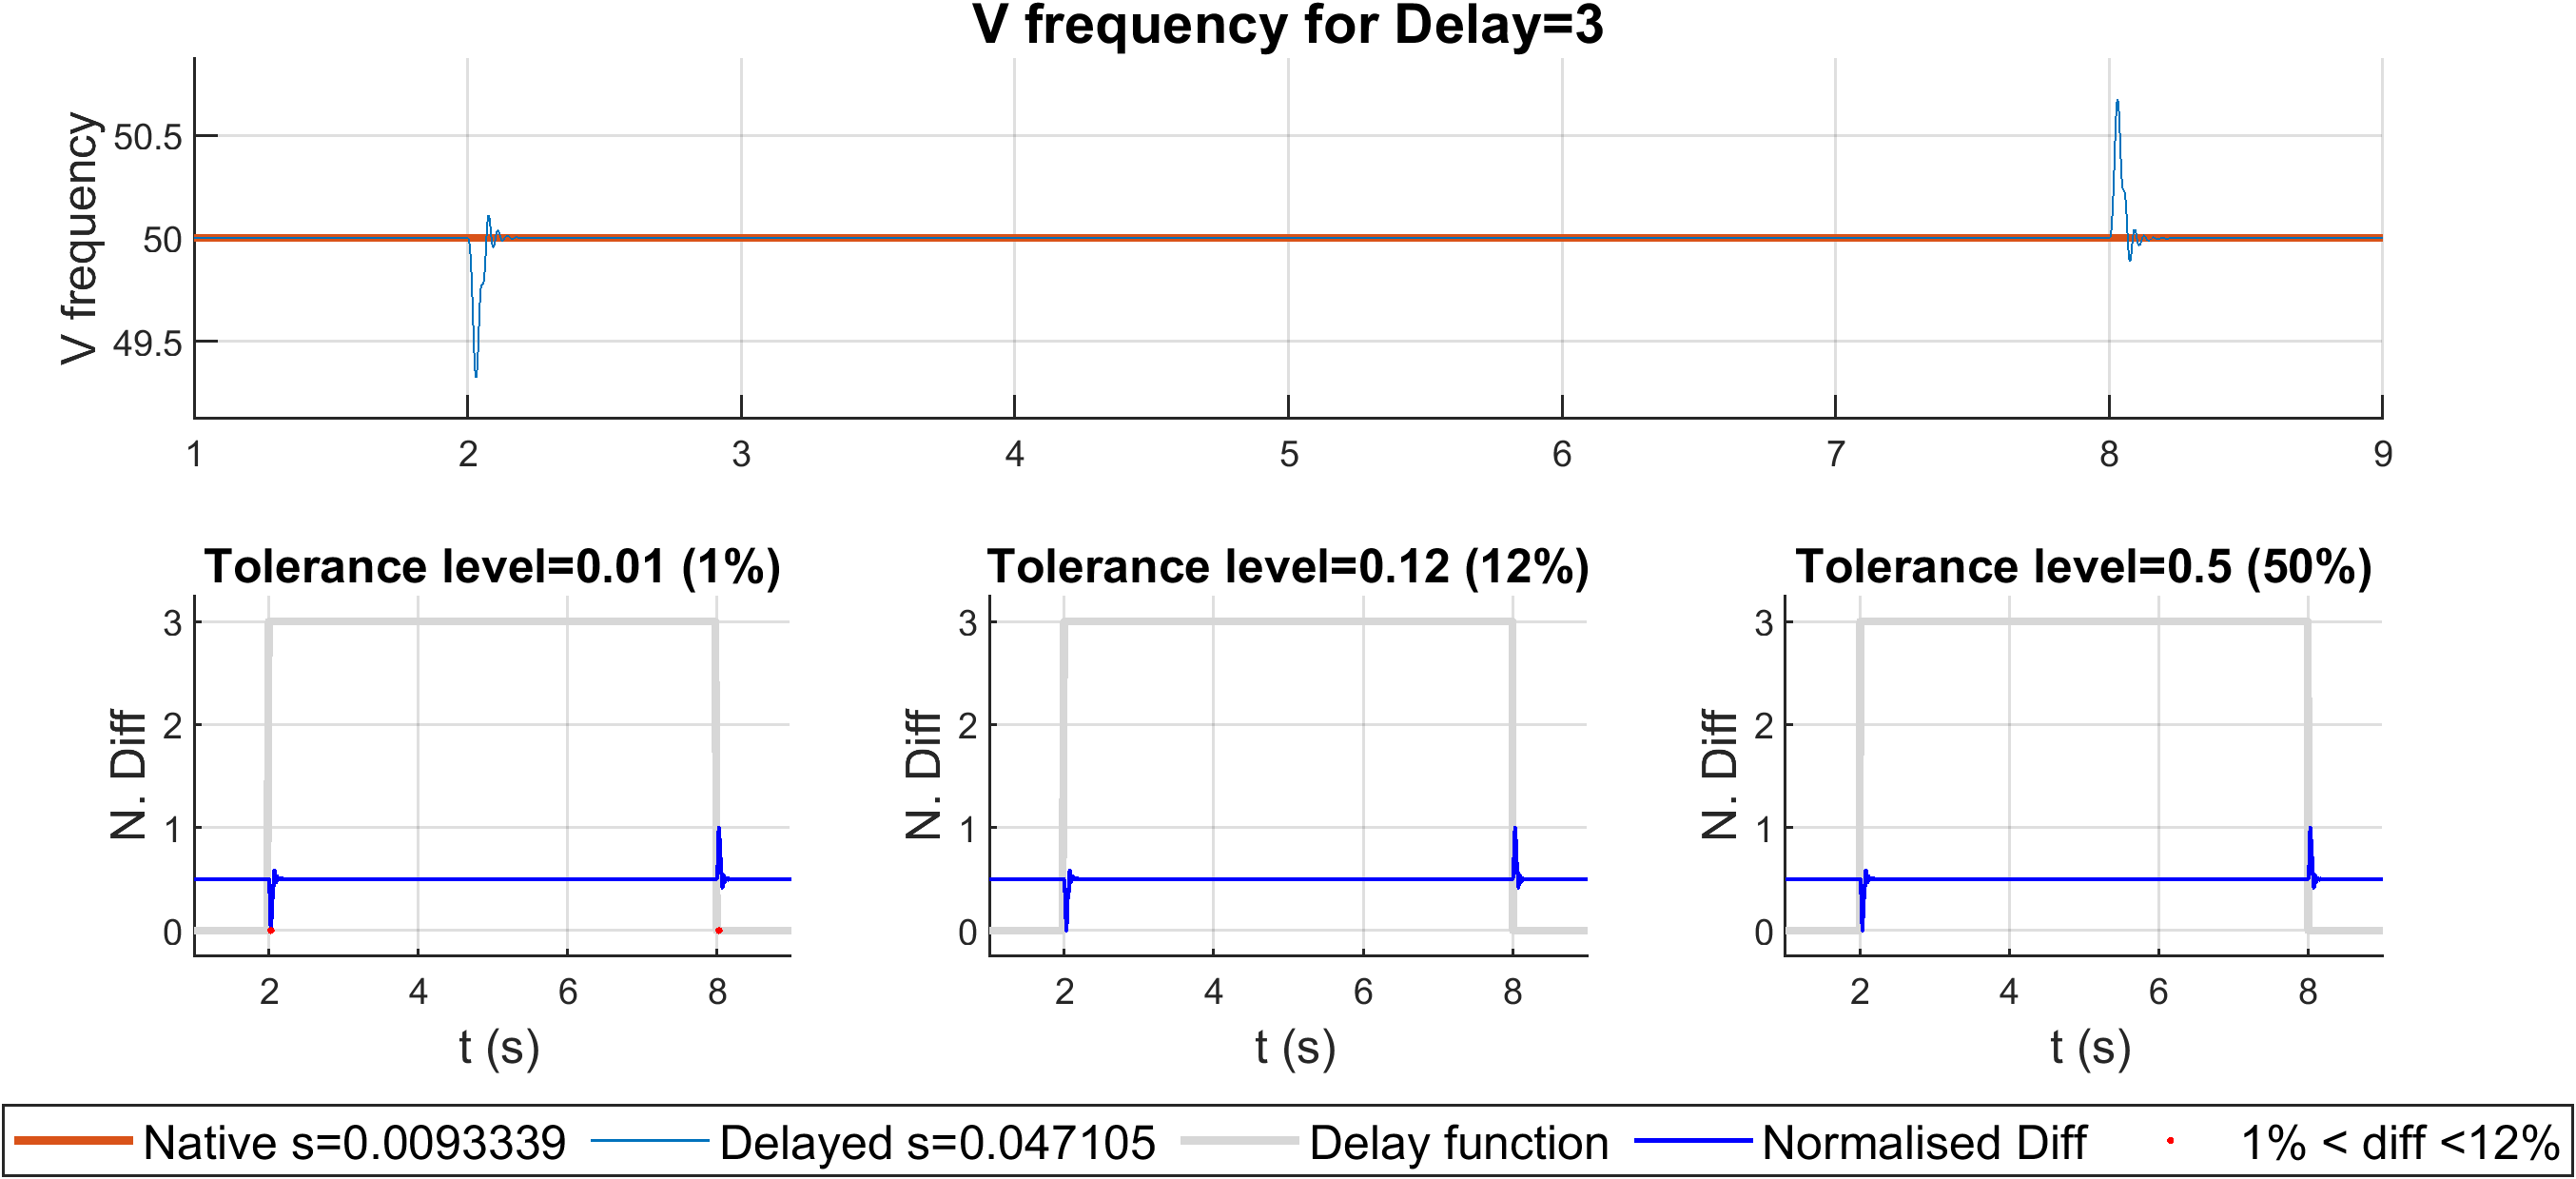
\includegraphics[width=0.95\textwidth]{PMUsim-figures/DelayOf_3/Instant_vFrequency.png}}


  \end{tabular}
\label{fig:VoltageInstantDelayThree}
\caption{Results for Voltage Output for Instant Delay equal to Three }
\end{figure}

\newpage
\begin{figure}[H]
\begin{tabular}{c}
  \fbox{  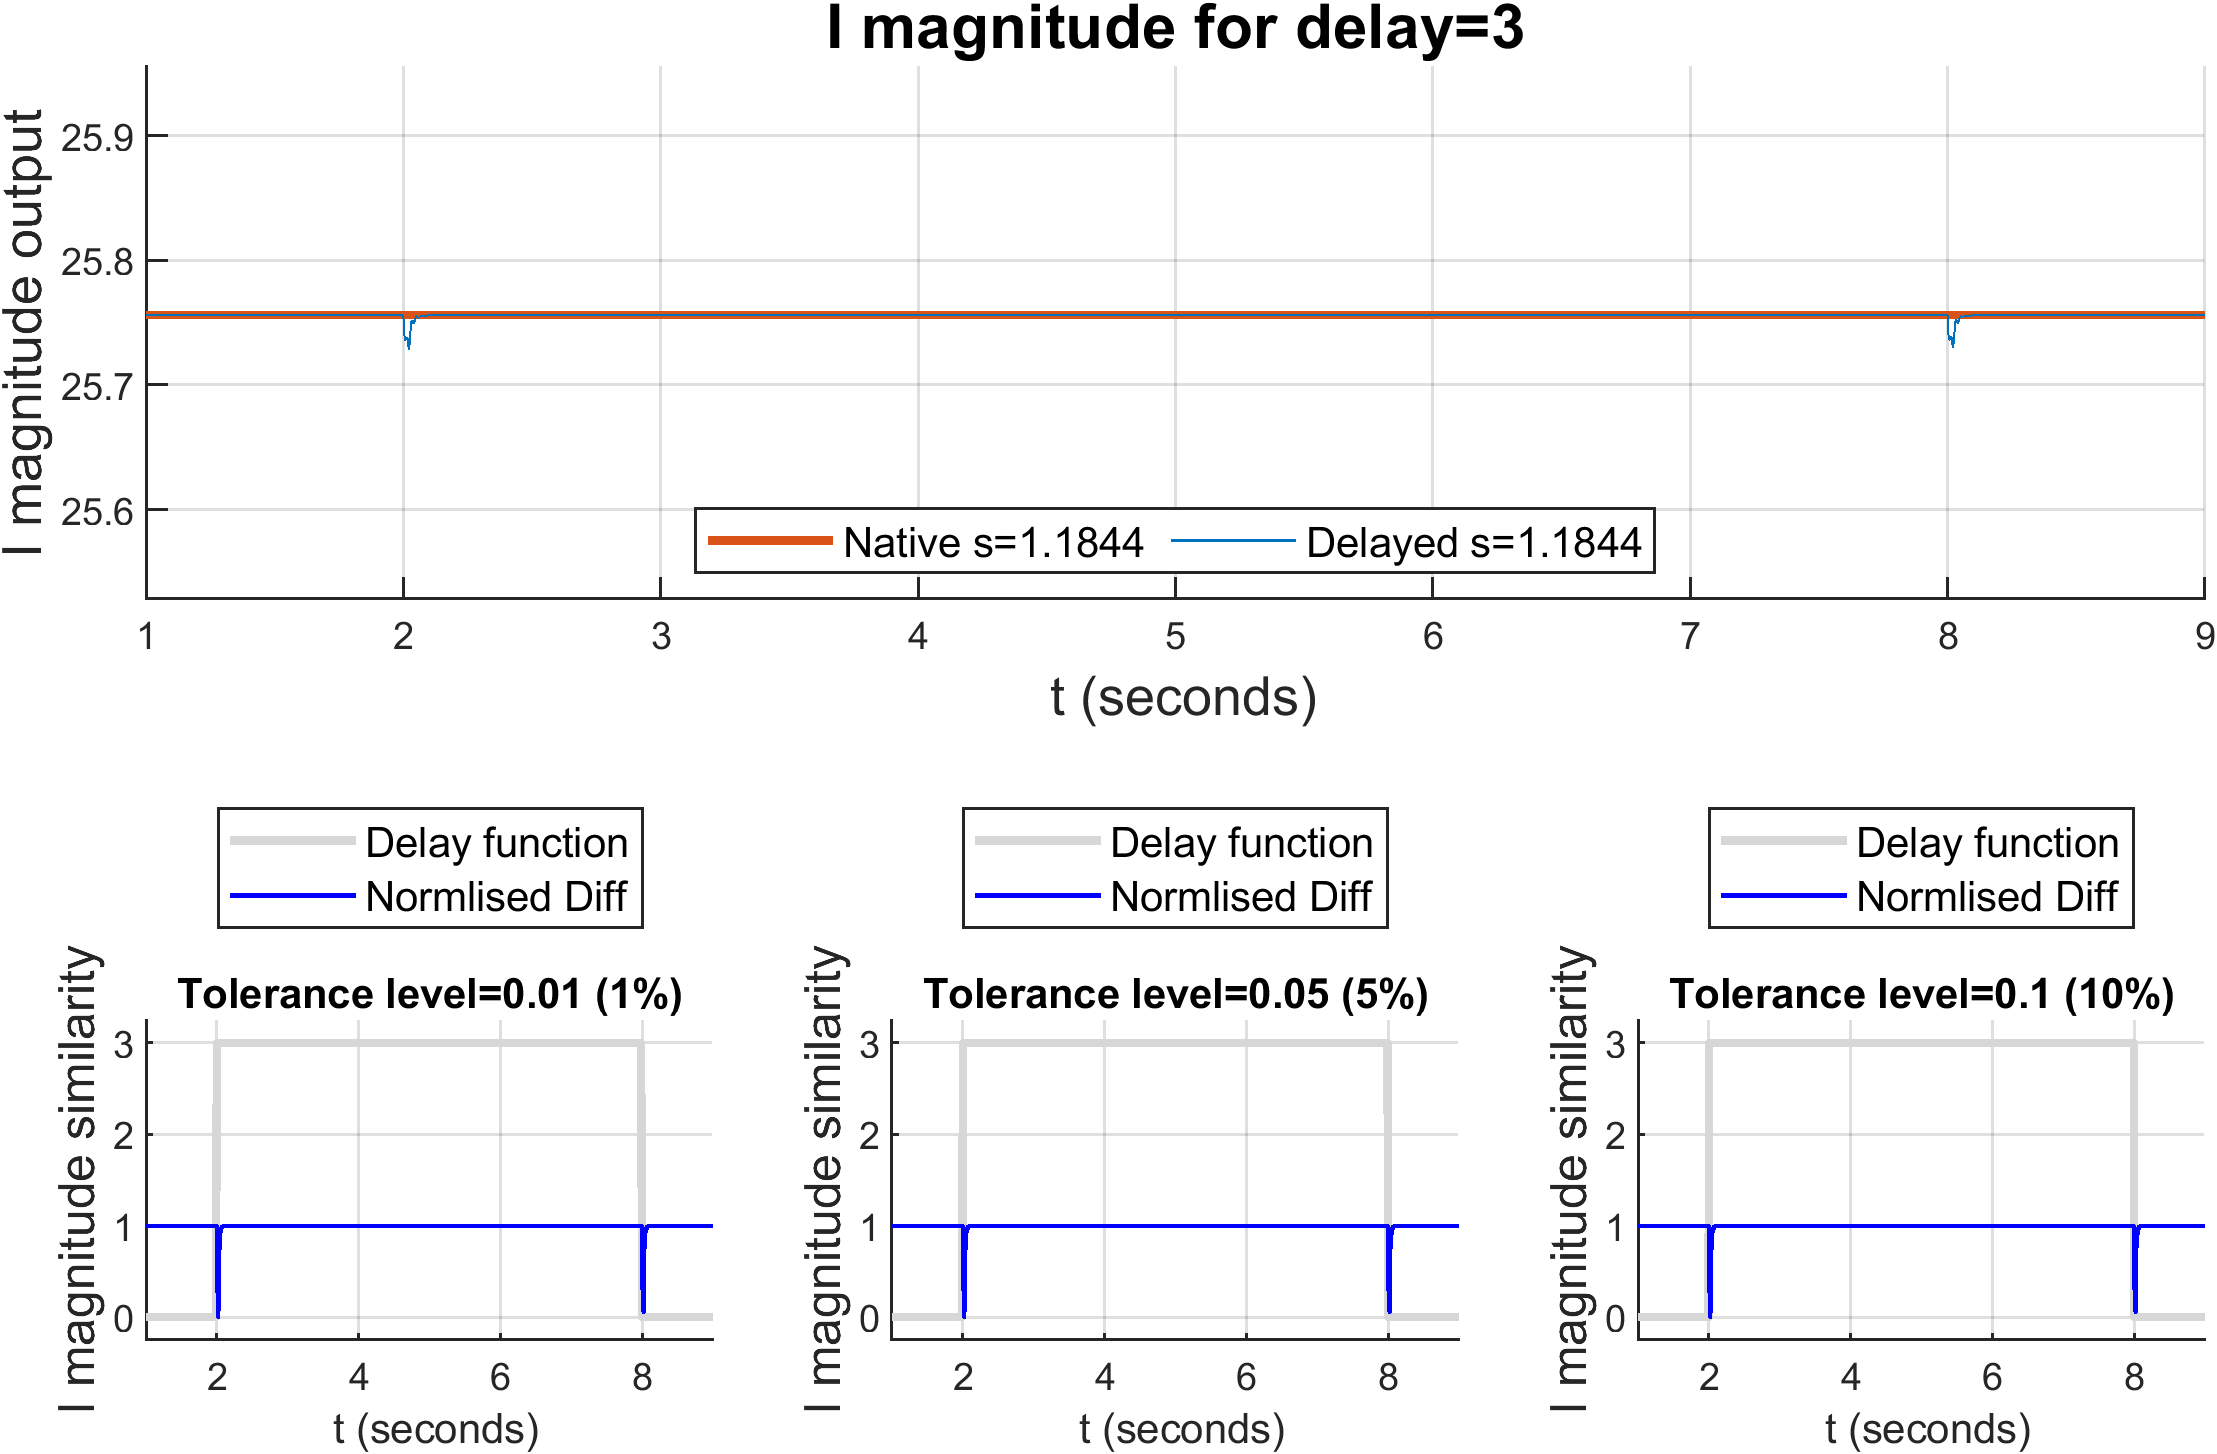
\includegraphics[width=0.95\textwidth]{PMUsim-figures/DelayOf_3/Instant_iMagnitude.png}} \\ 
   \fbox{     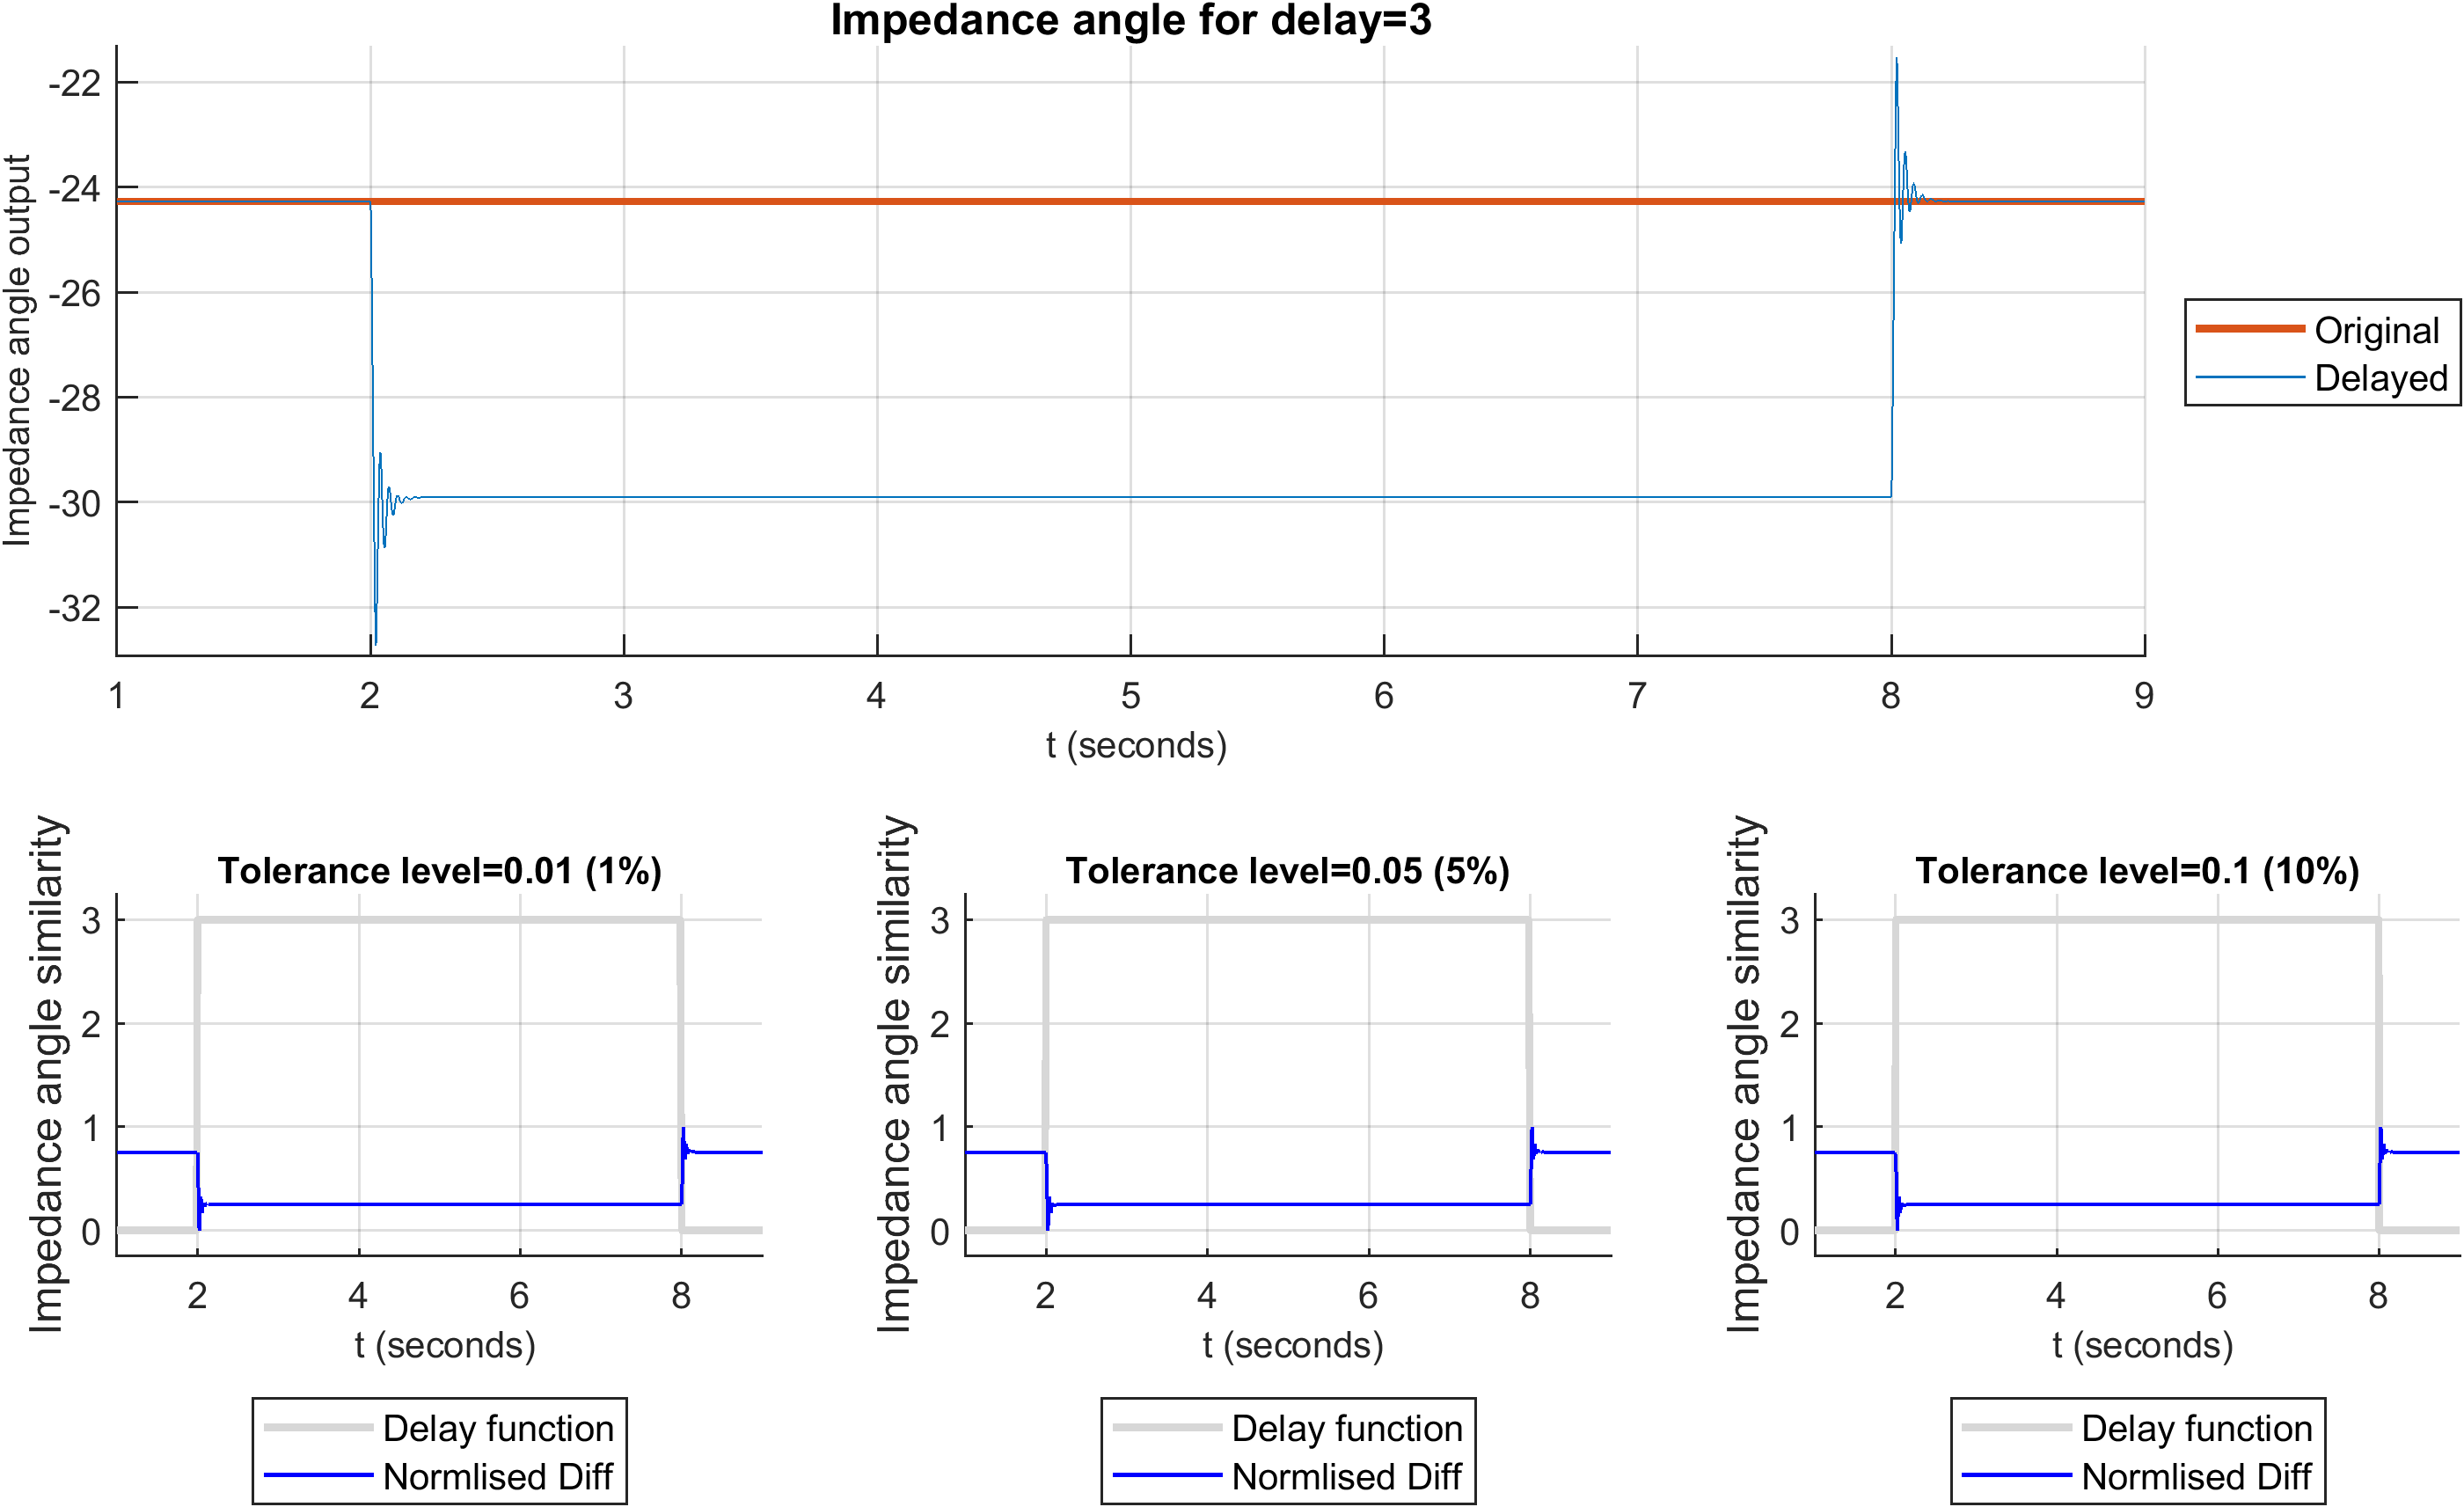
\includegraphics[width=0.95\textwidth]{PMUsim-figures/DelayOf_3/Instant_iAngle.png}} \\    
   \fbox{    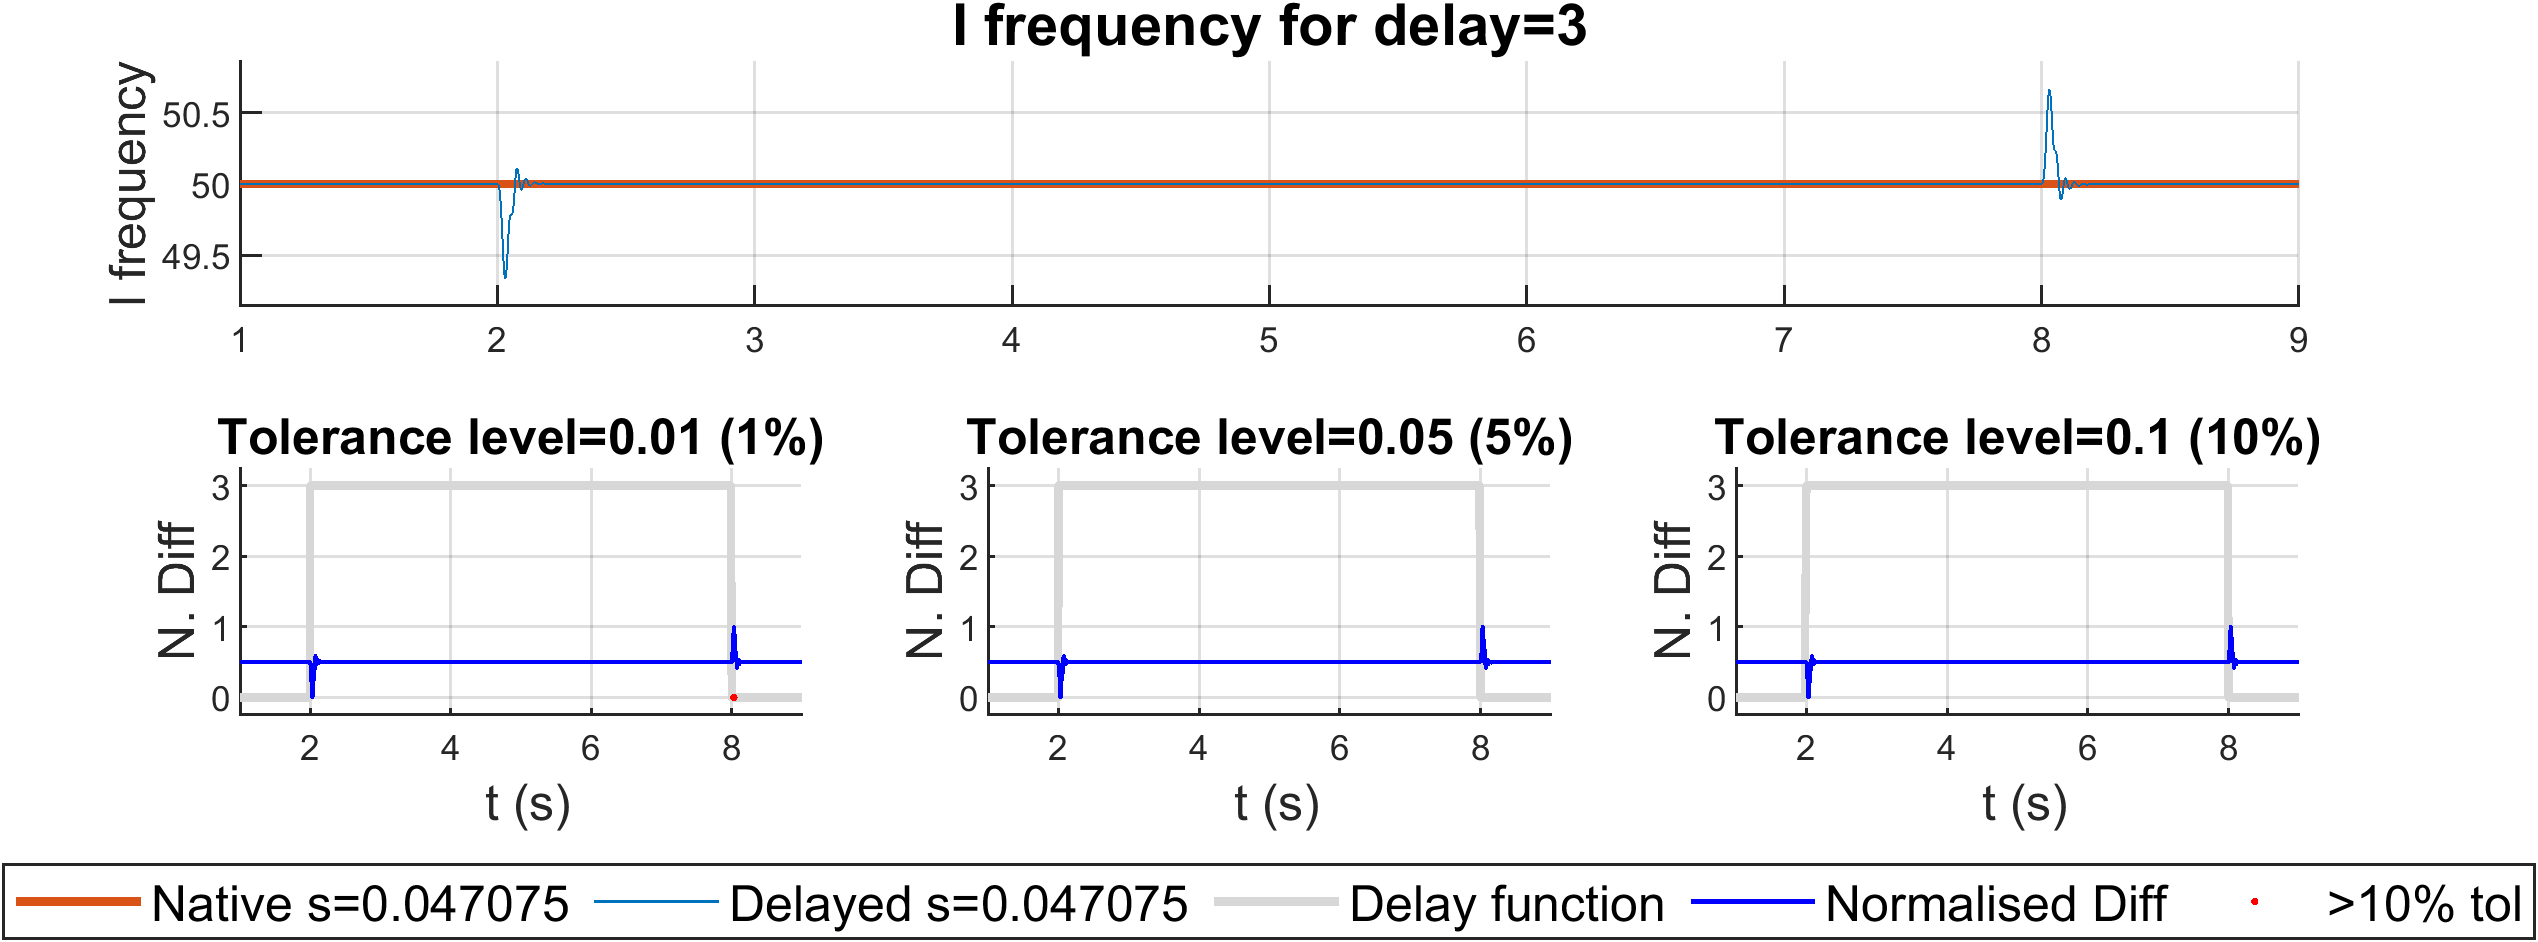
\includegraphics[width=0.95\textwidth]{PMUsim-figures/DelayOf_3/Instant_iFrequency.png}}


  \end{tabular}
\label{fig:ImpedanceInstantDelayThree}
\caption{Results for Impedance Output for Instant Delay equal to Three }
\end{figure}






\newpage
\begin{figure}[H]
\begin{tabular}{c}
  \fbox{  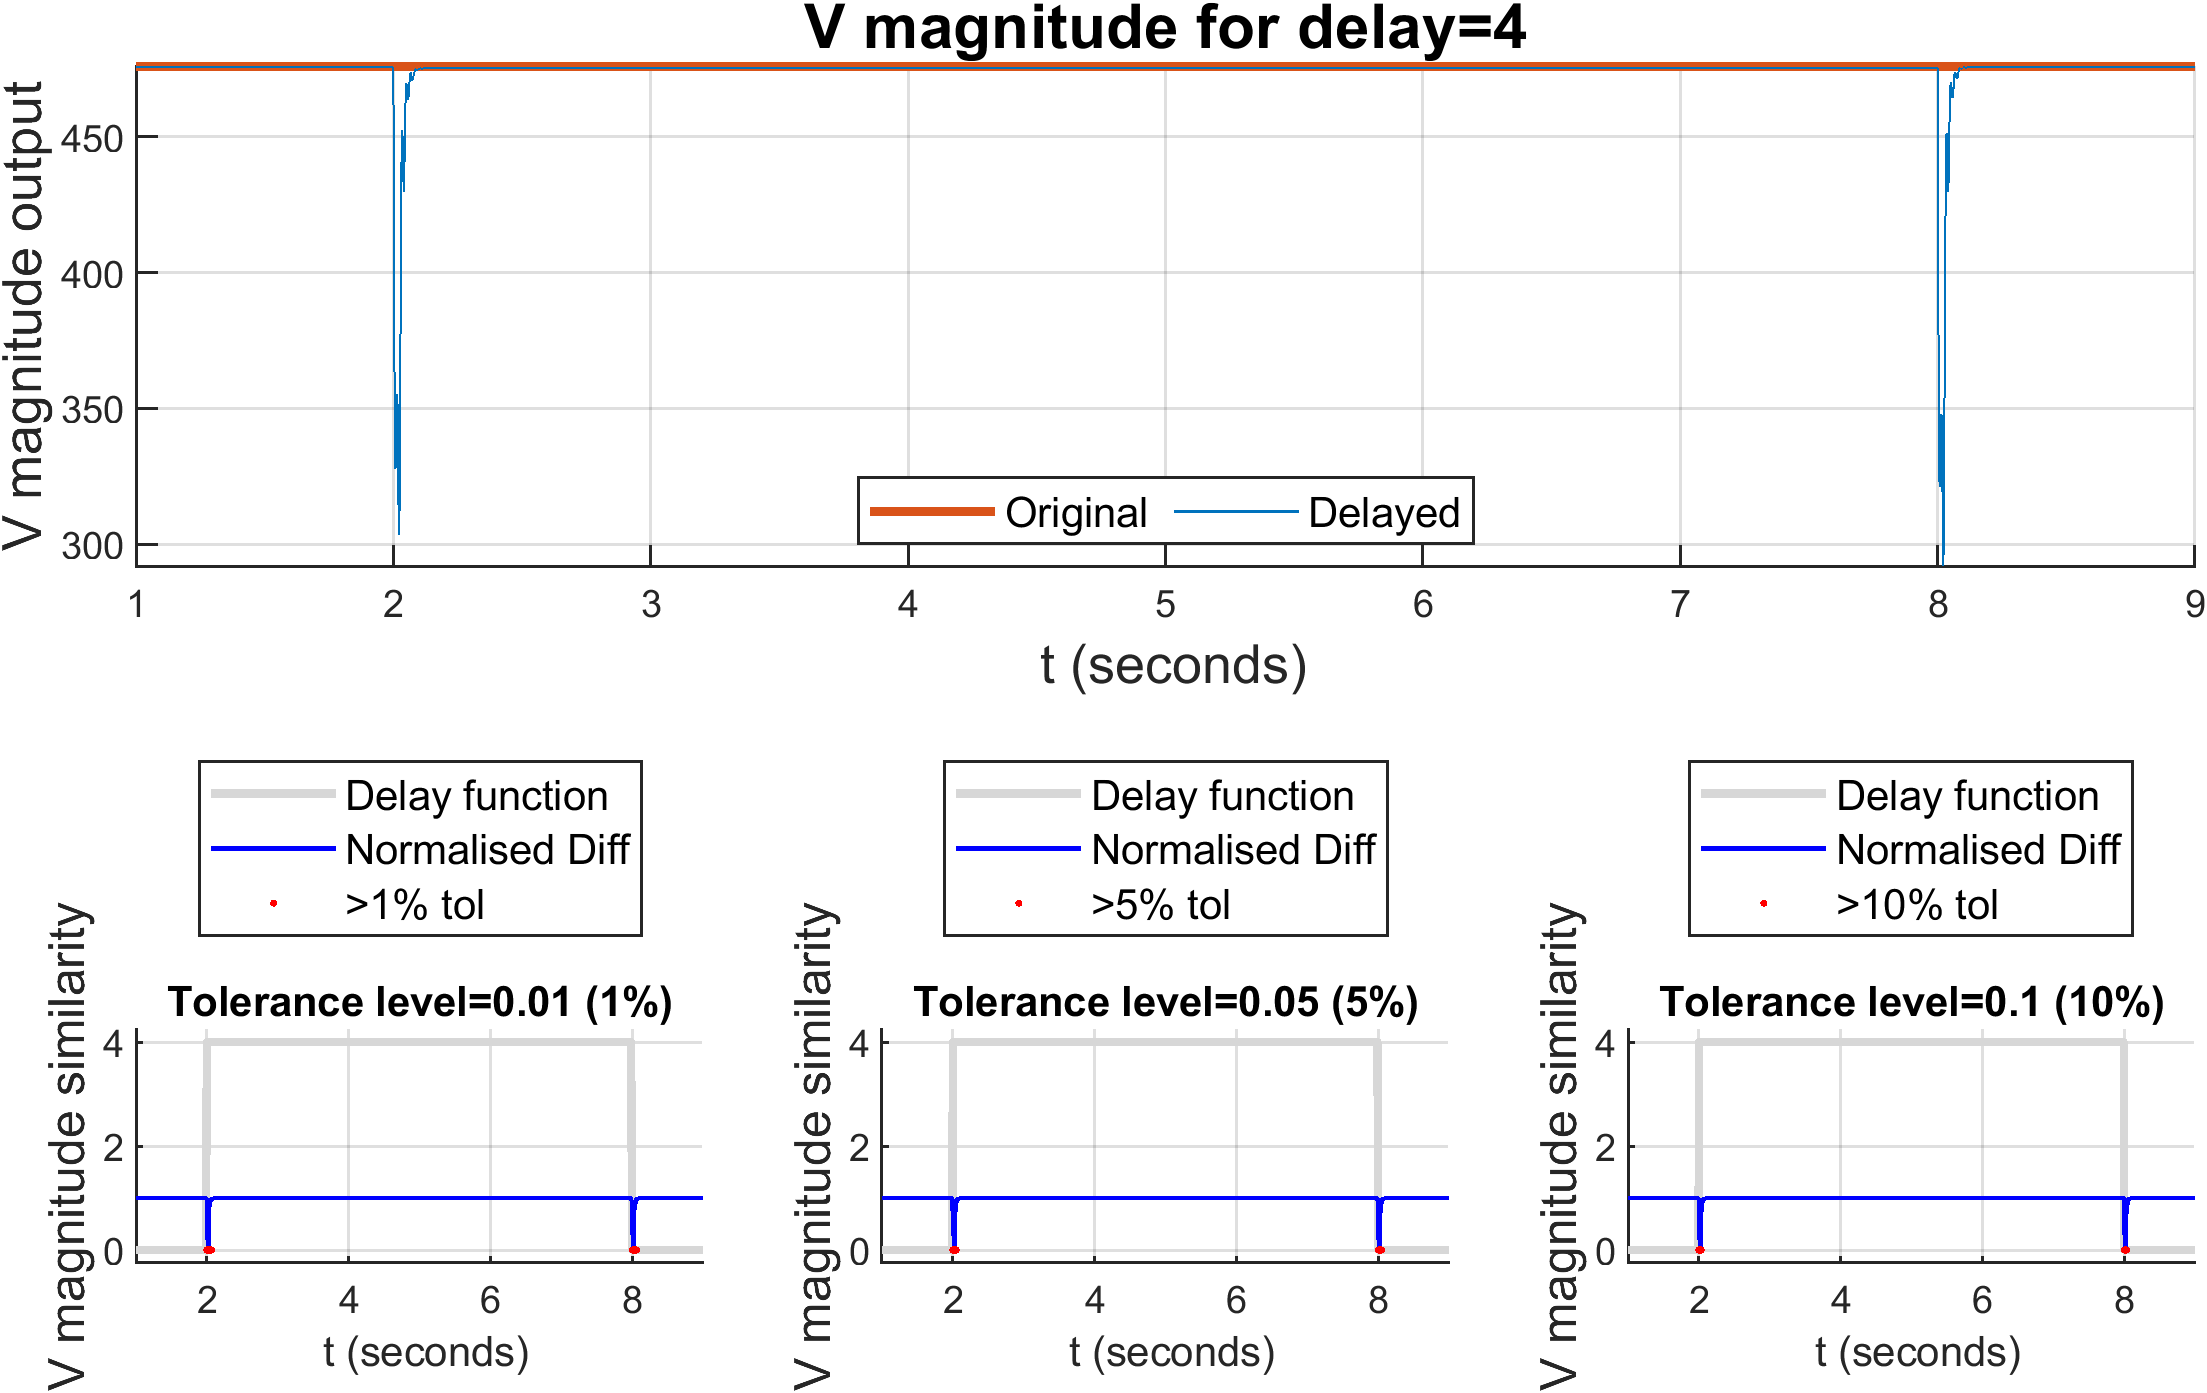
\includegraphics[width=0.95\textwidth]{PMUsim-figures/DelayOf_4/Instant_vMagnitude.png}} \\ 
  \fbox{     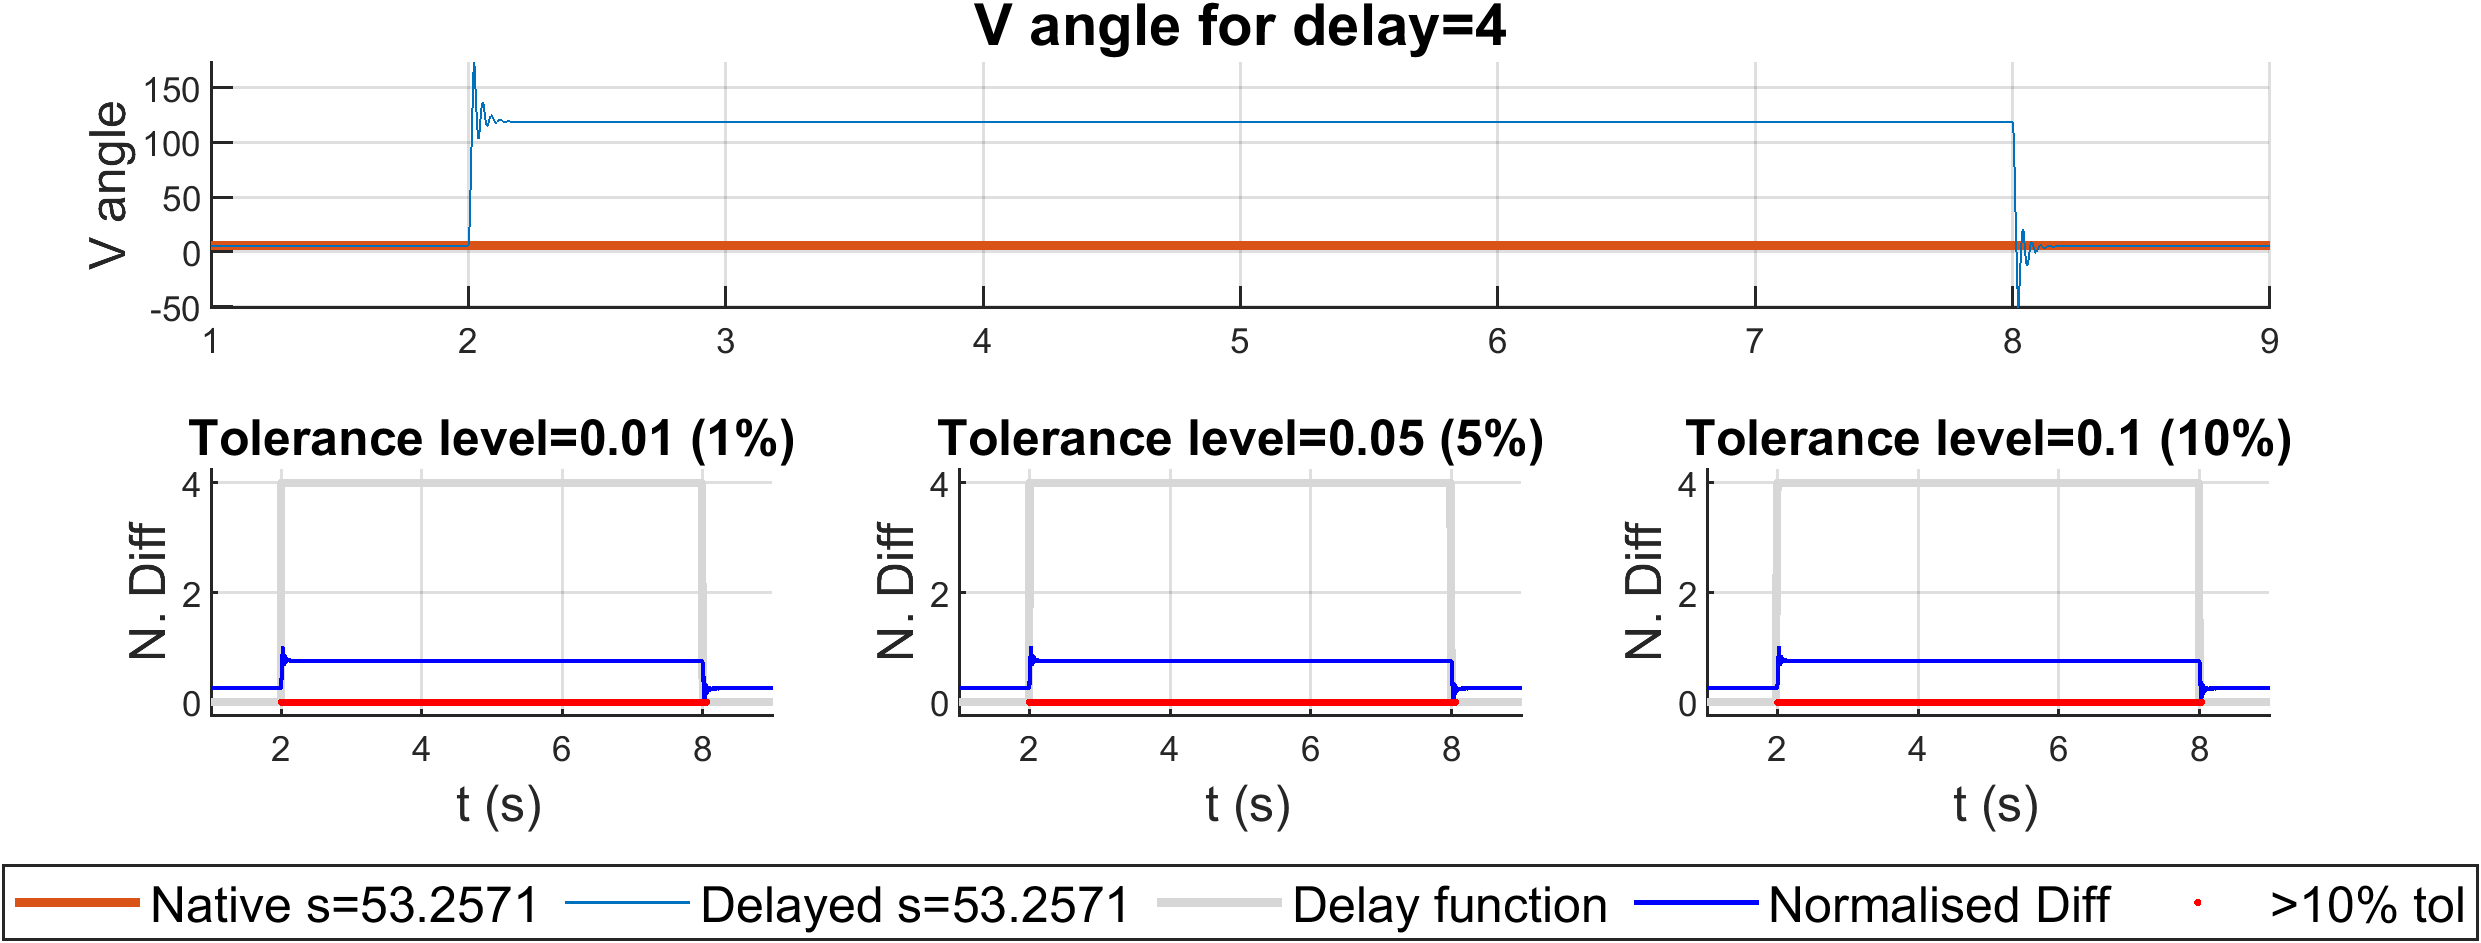
\includegraphics[width=0.95\textwidth]{PMUsim-figures/DelayOf_4/Instant_vAngle.png}} \\   
   \fbox{    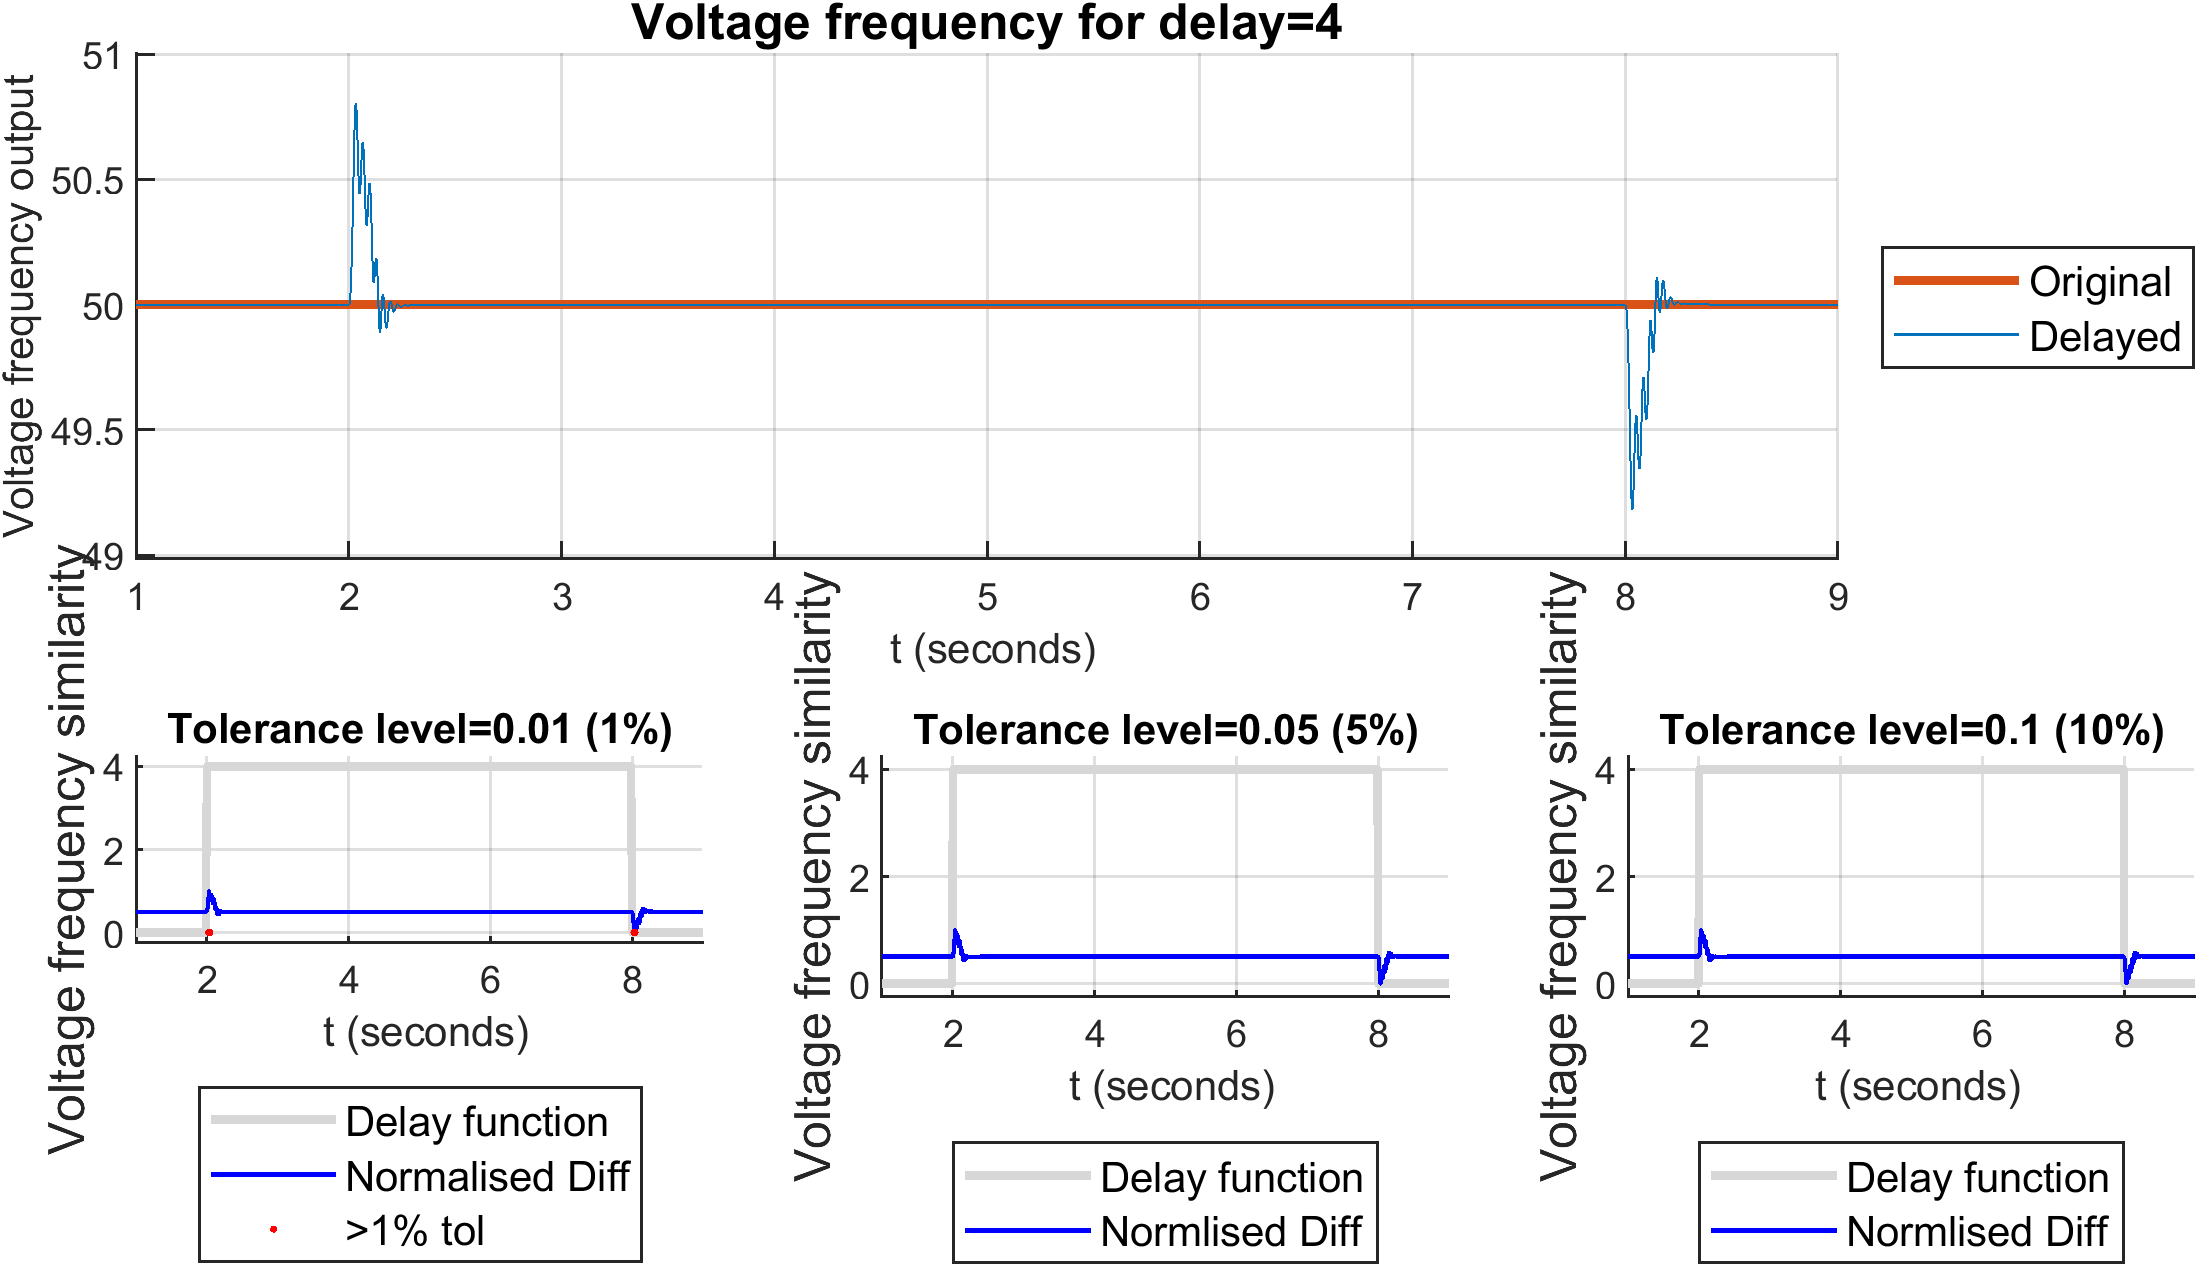
\includegraphics[width=0.95\textwidth]{PMUsim-figures/DelayOf_4/Instant_vFrequency.png}} 
 
  \end{tabular}
\label{fig:VoltageInstantDelayFour}
\caption{Results for Voltage Output for Instant Delay equal to Four }
\end{figure}

\newpage
\begin{figure}[H]
\begin{tabular}{c}
  \fbox{  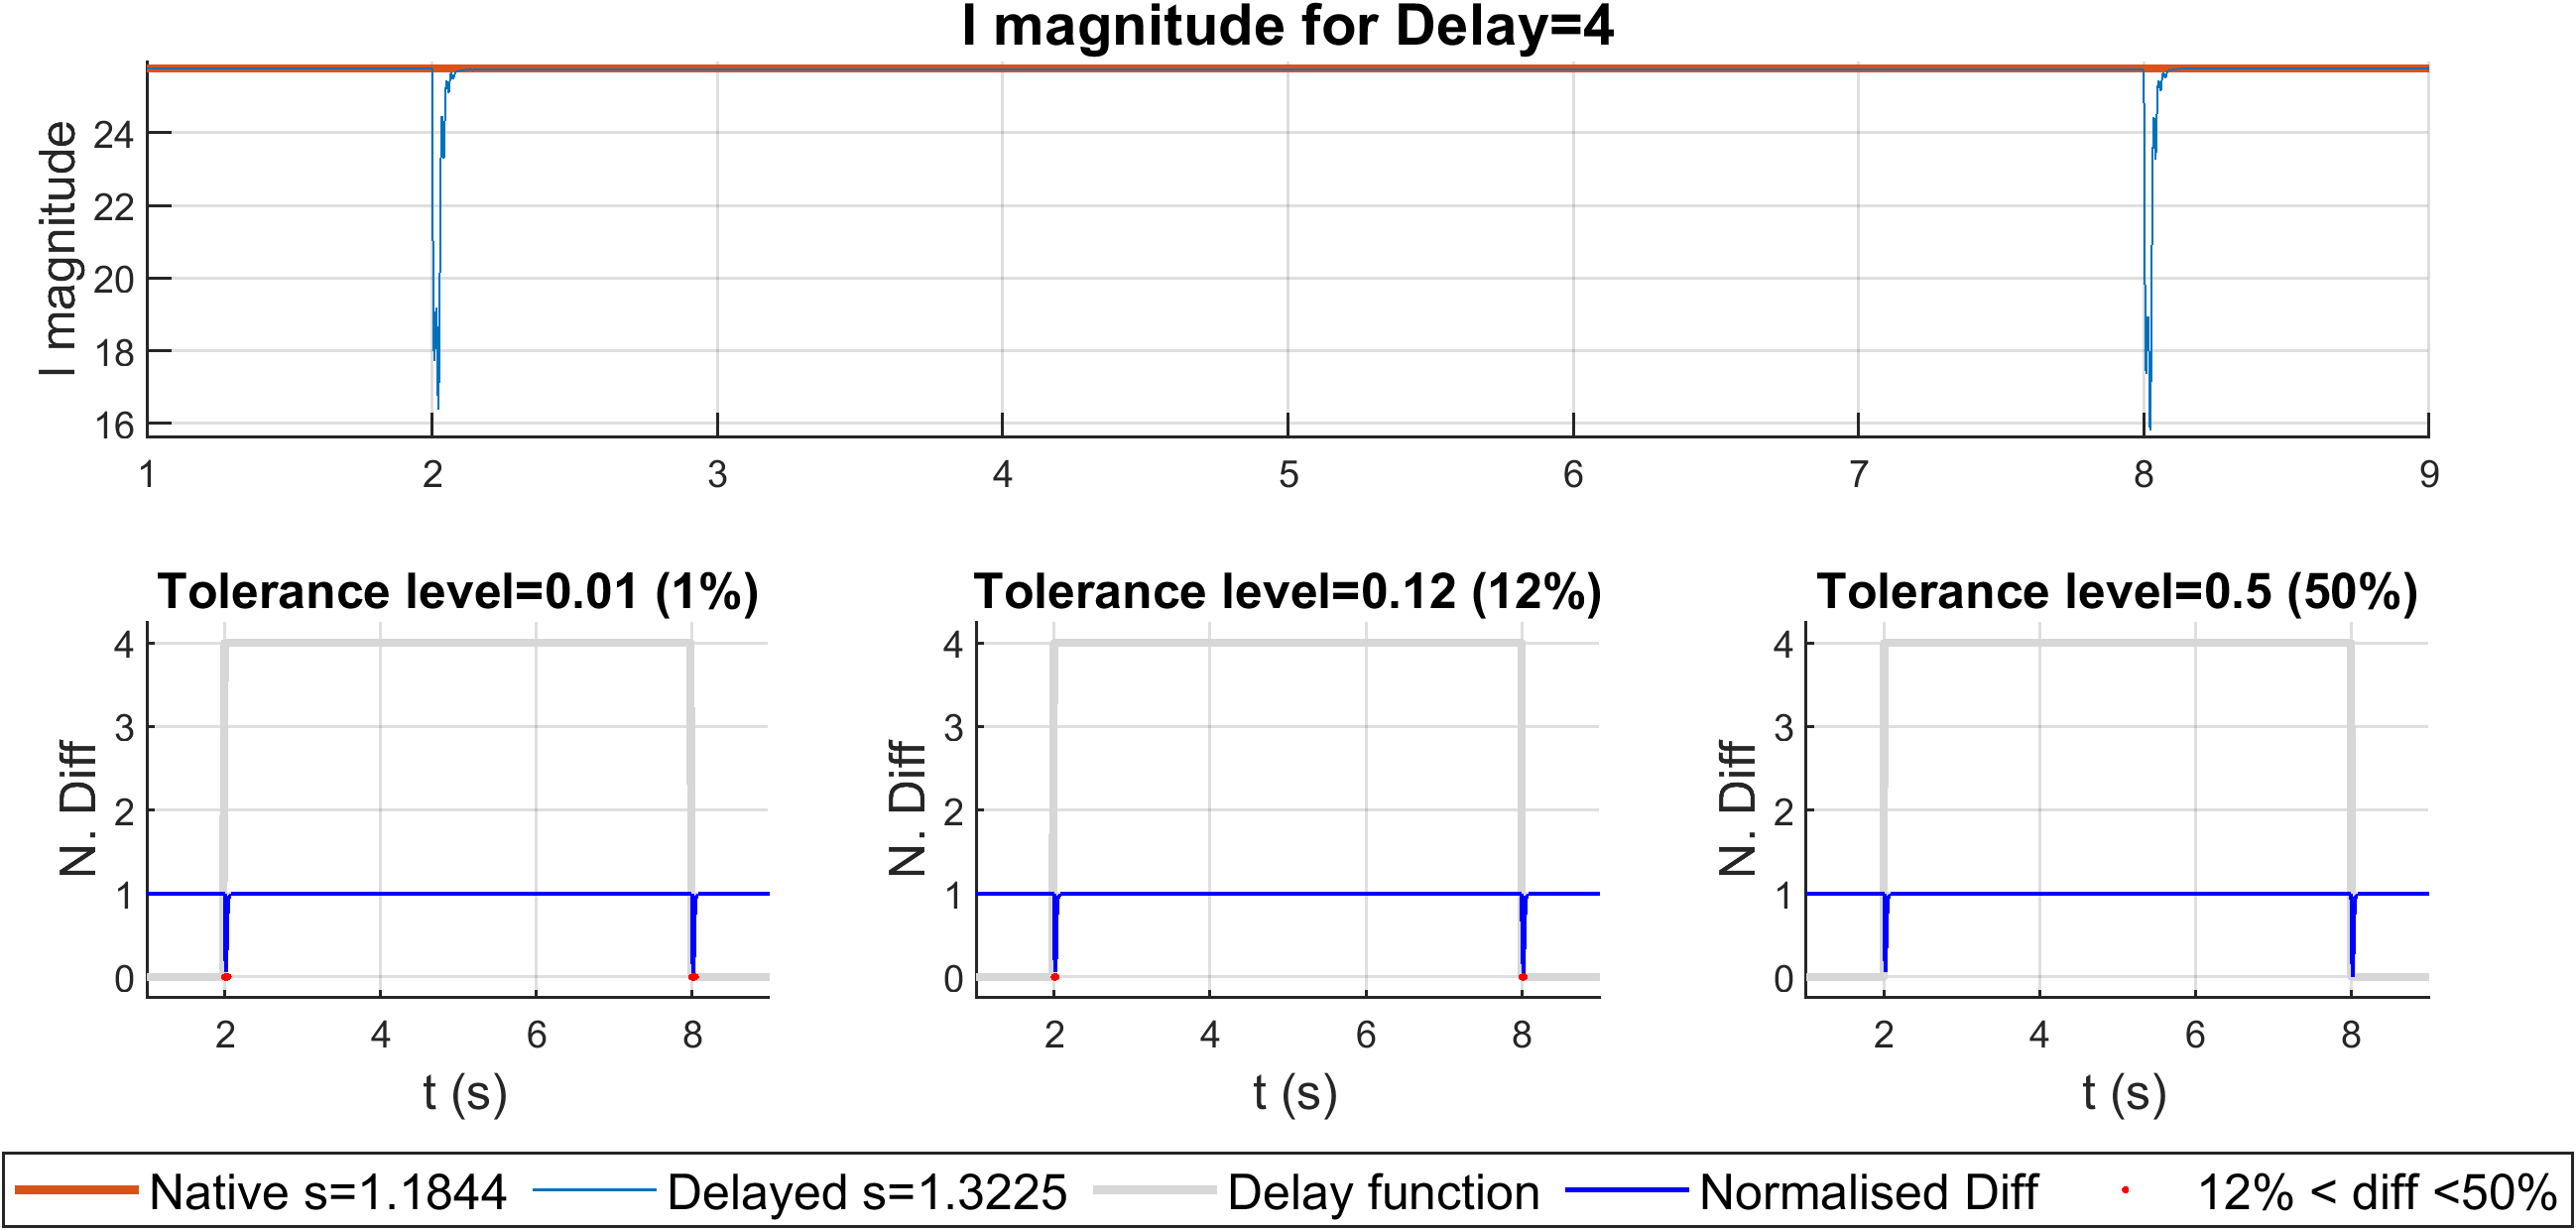
\includegraphics[width=0.95\textwidth]{PMUsim-figures/DelayOf_4/Instant_iMagnitude.png}} \\ 
   \fbox{     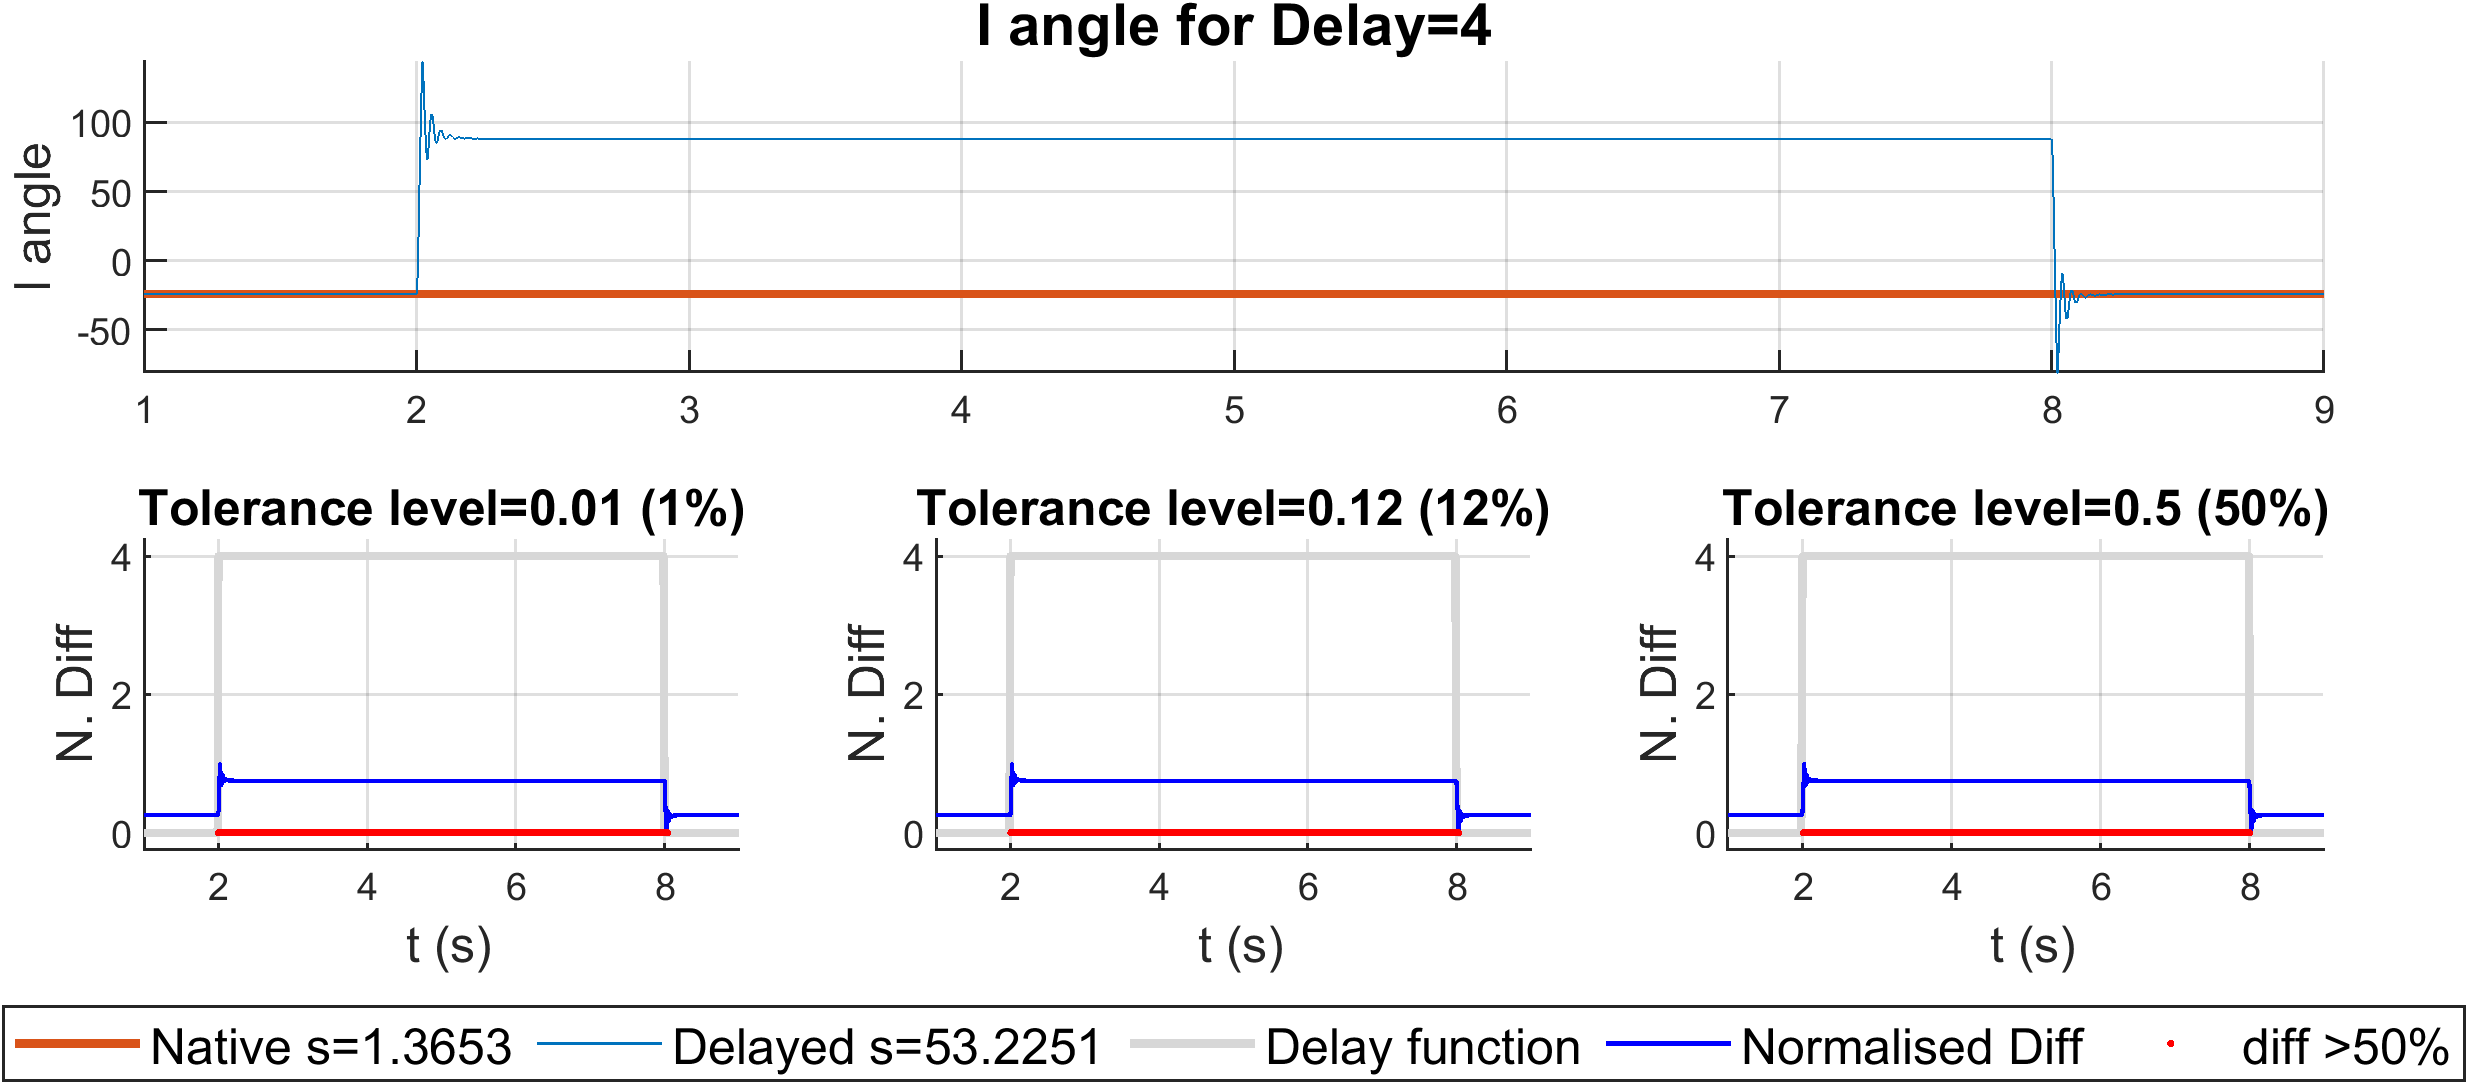
\includegraphics[width=0.95\textwidth]{PMUsim-figures/DelayOf_4/Instant_iAngle.png}} \\    
   \fbox{    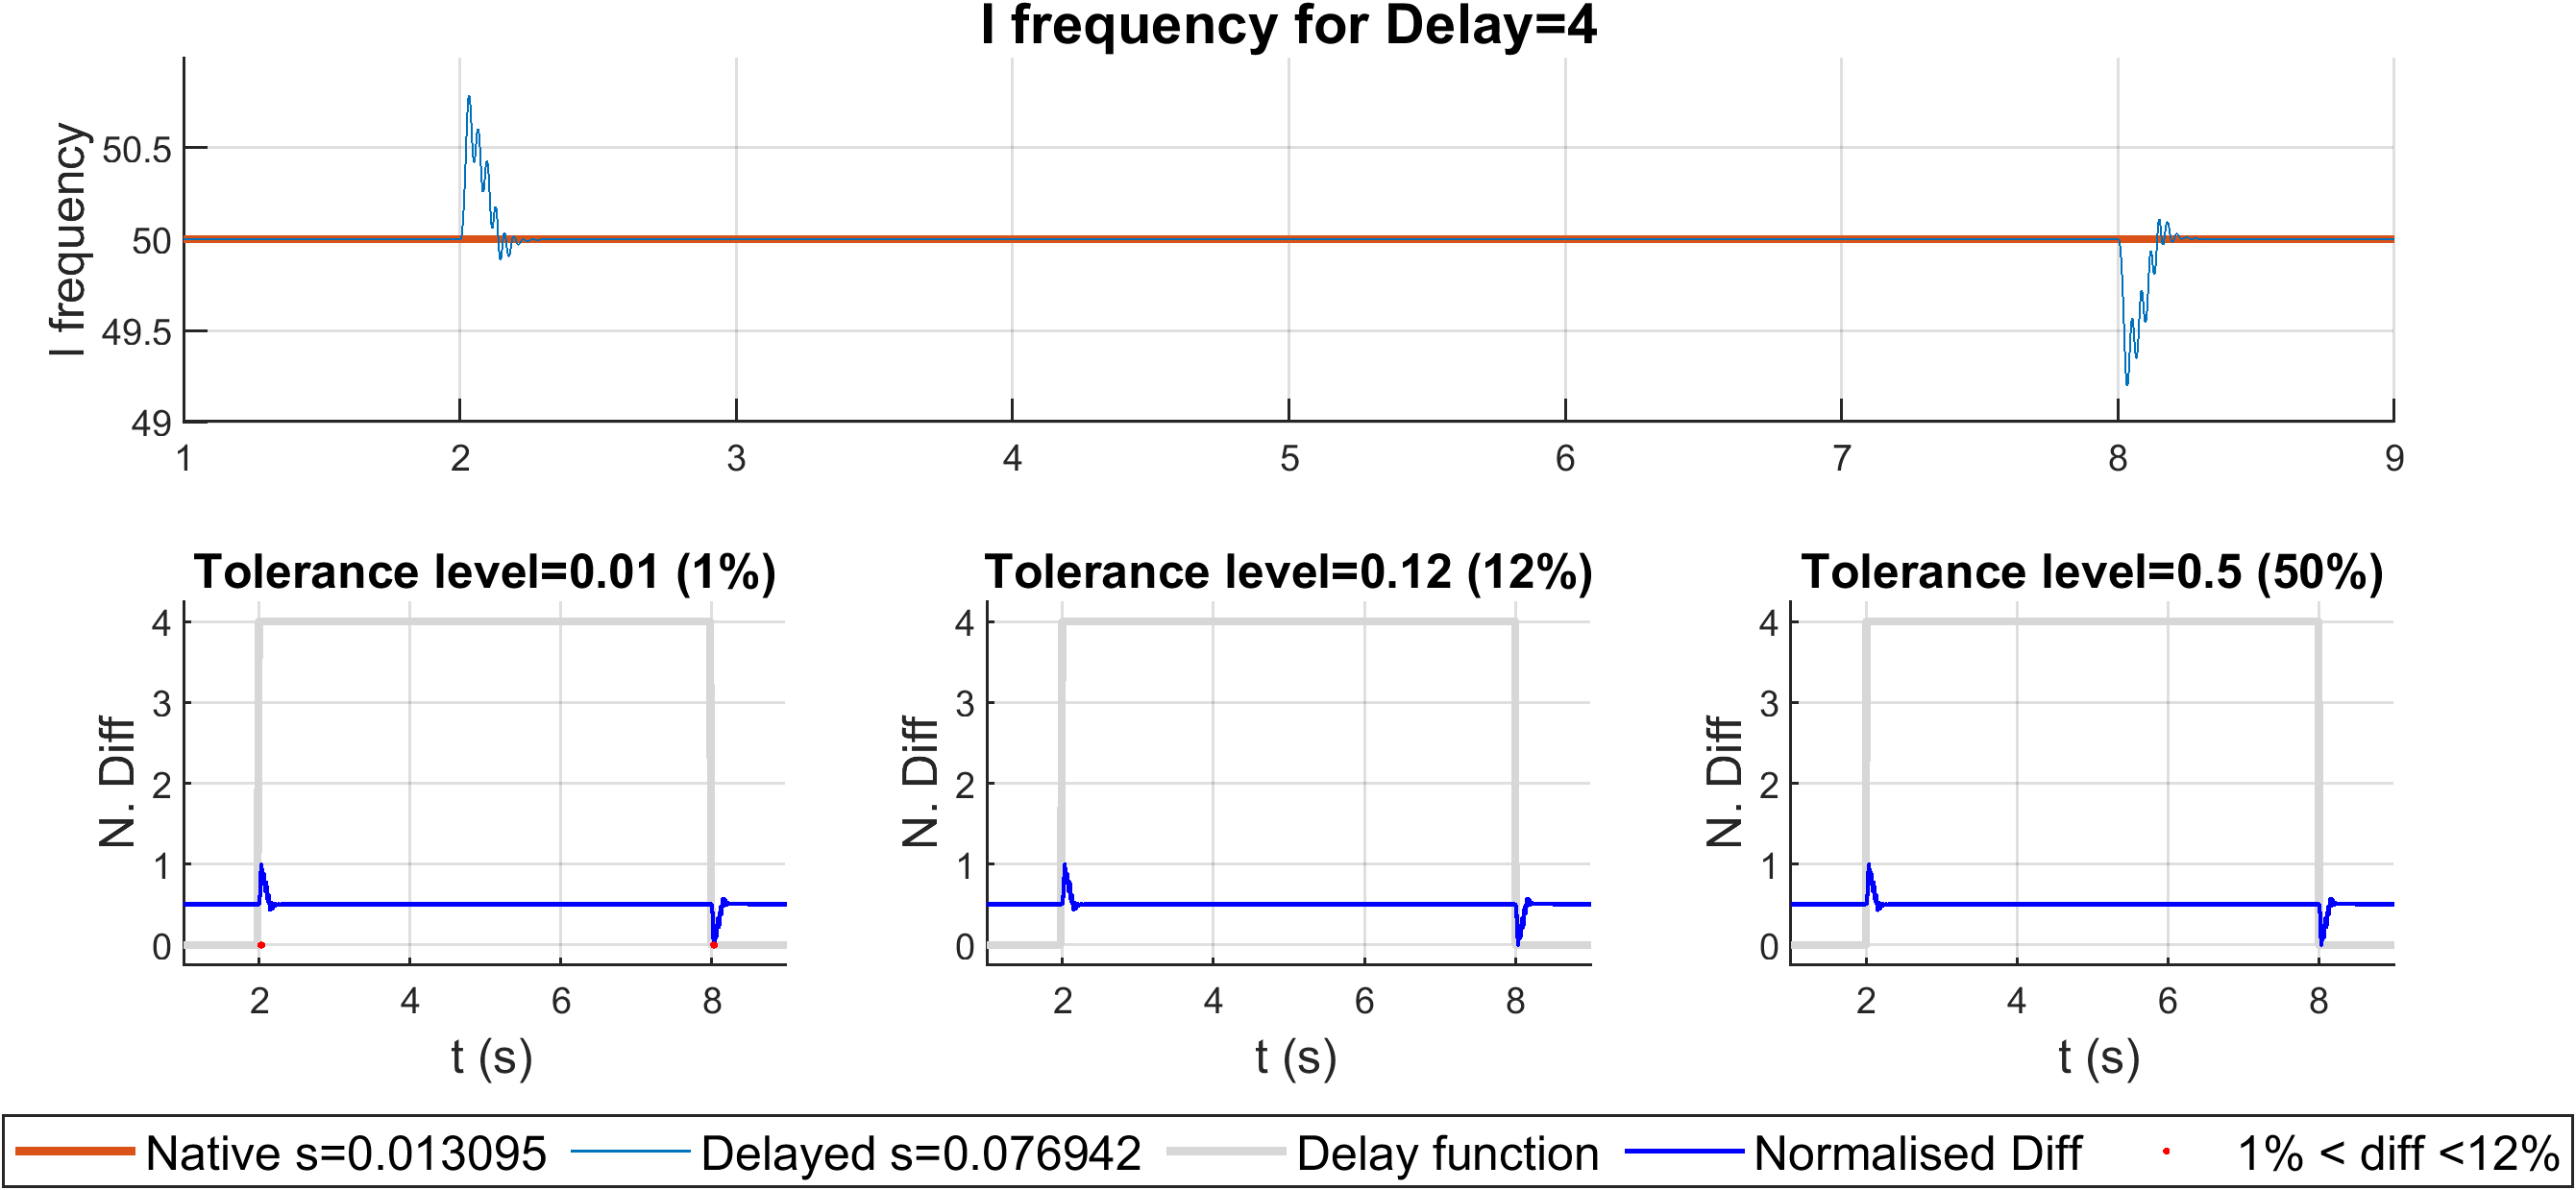
\includegraphics[width=0.95\textwidth]{PMUsim-figures/DelayOf_4/Instant_iFrequency.png}}


  \end{tabular}
\label{fig:ImpedanceInstantDelayFour}
\caption{Results for Impedance Output for Instant Delay equal to Four }
\end{figure}




\newpage
\begin{figure}[H]
\begin{tabular}{c}
  \fbox{  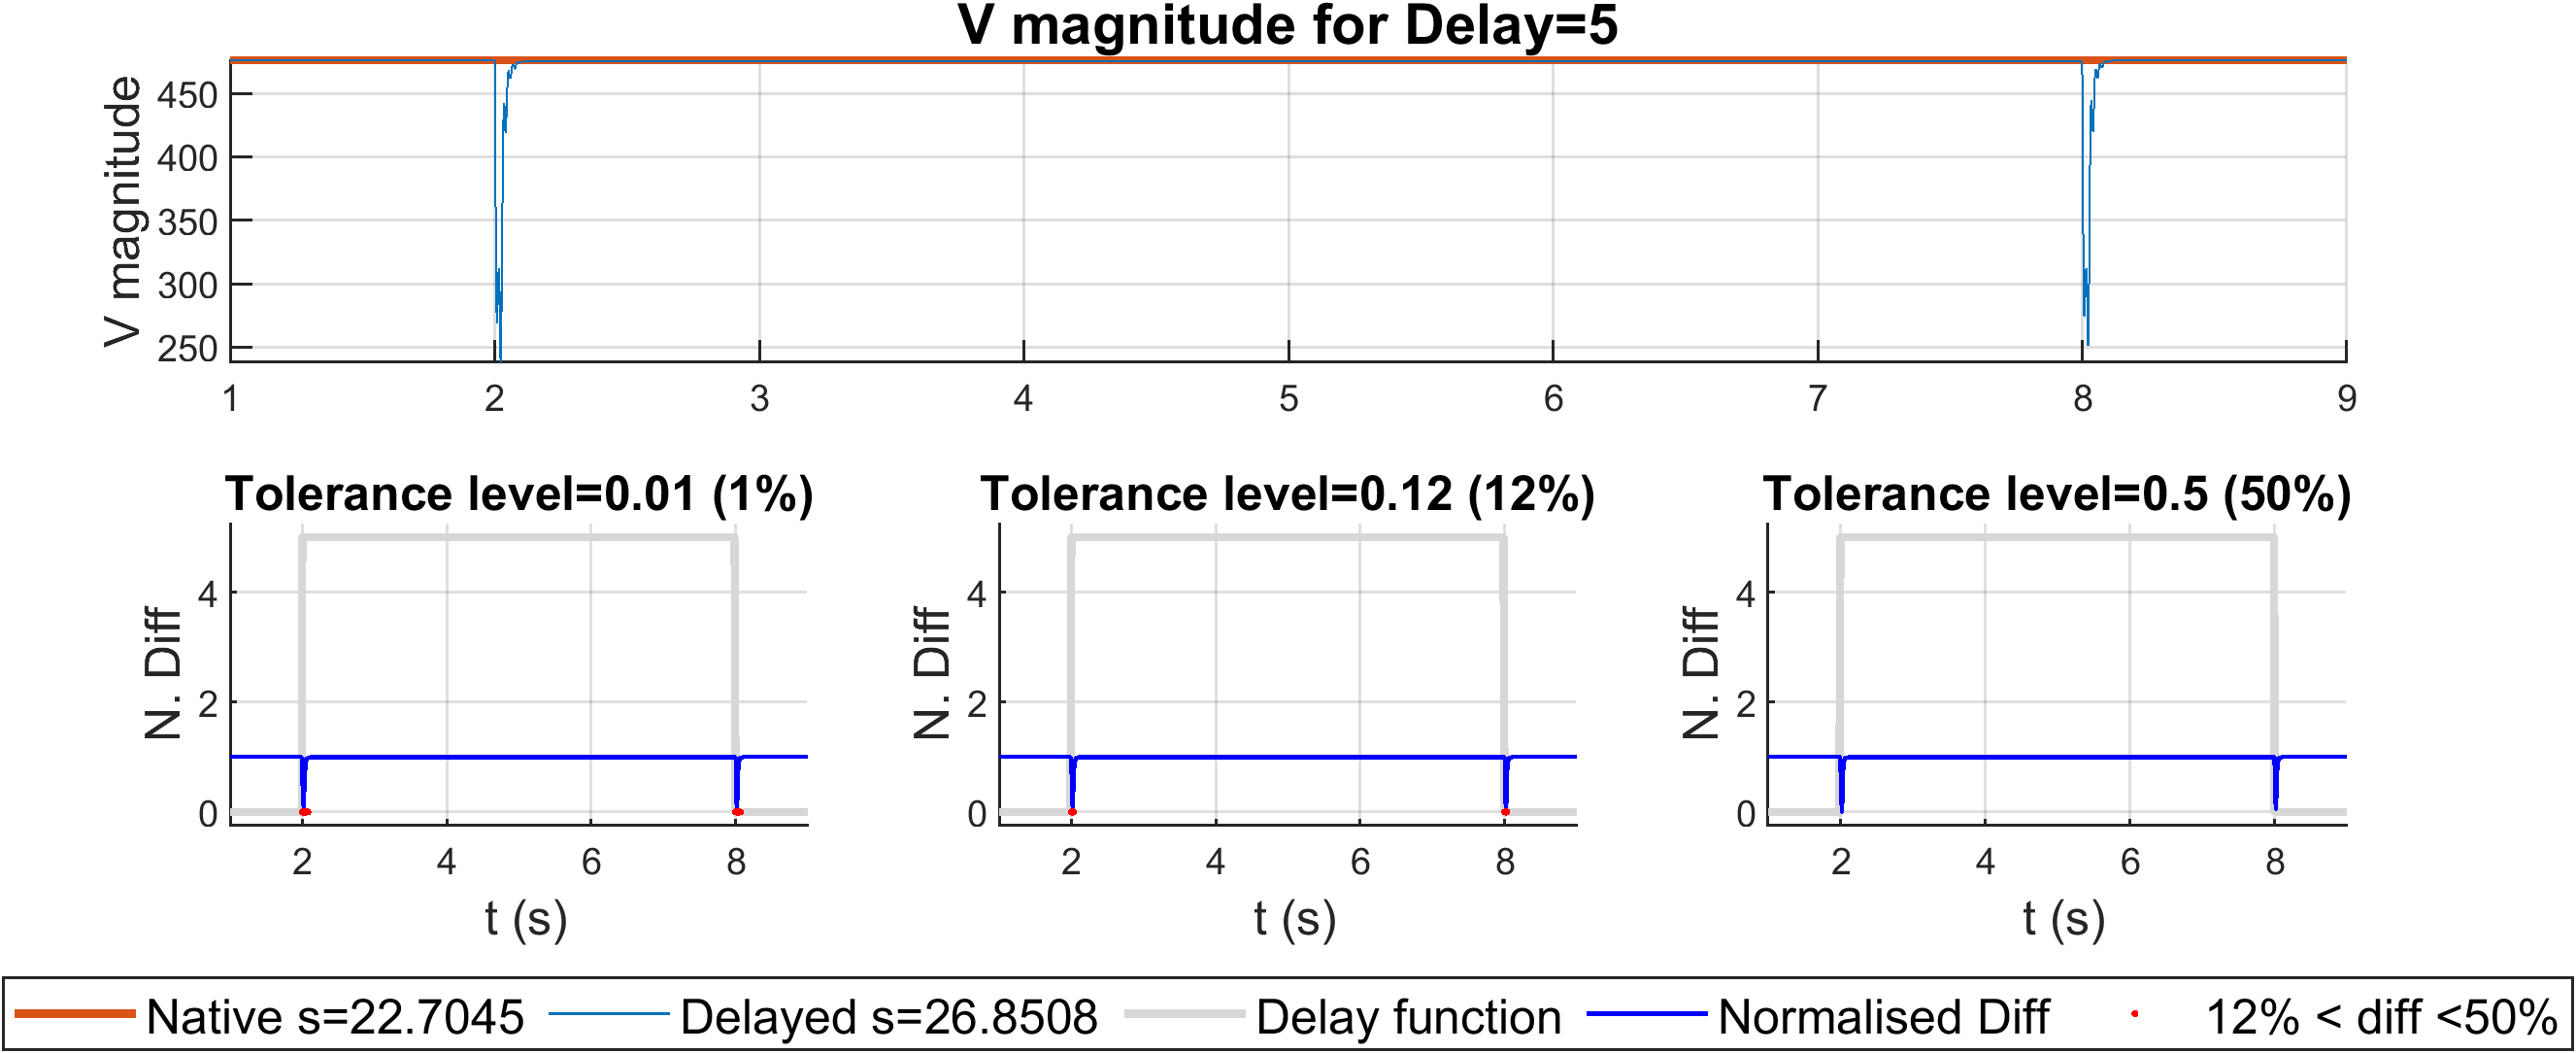
\includegraphics[width=0.95\textwidth]{PMUsim-figures/DelayOf_5/Instant_vMagnitude.png}} \\ 
    \fbox{     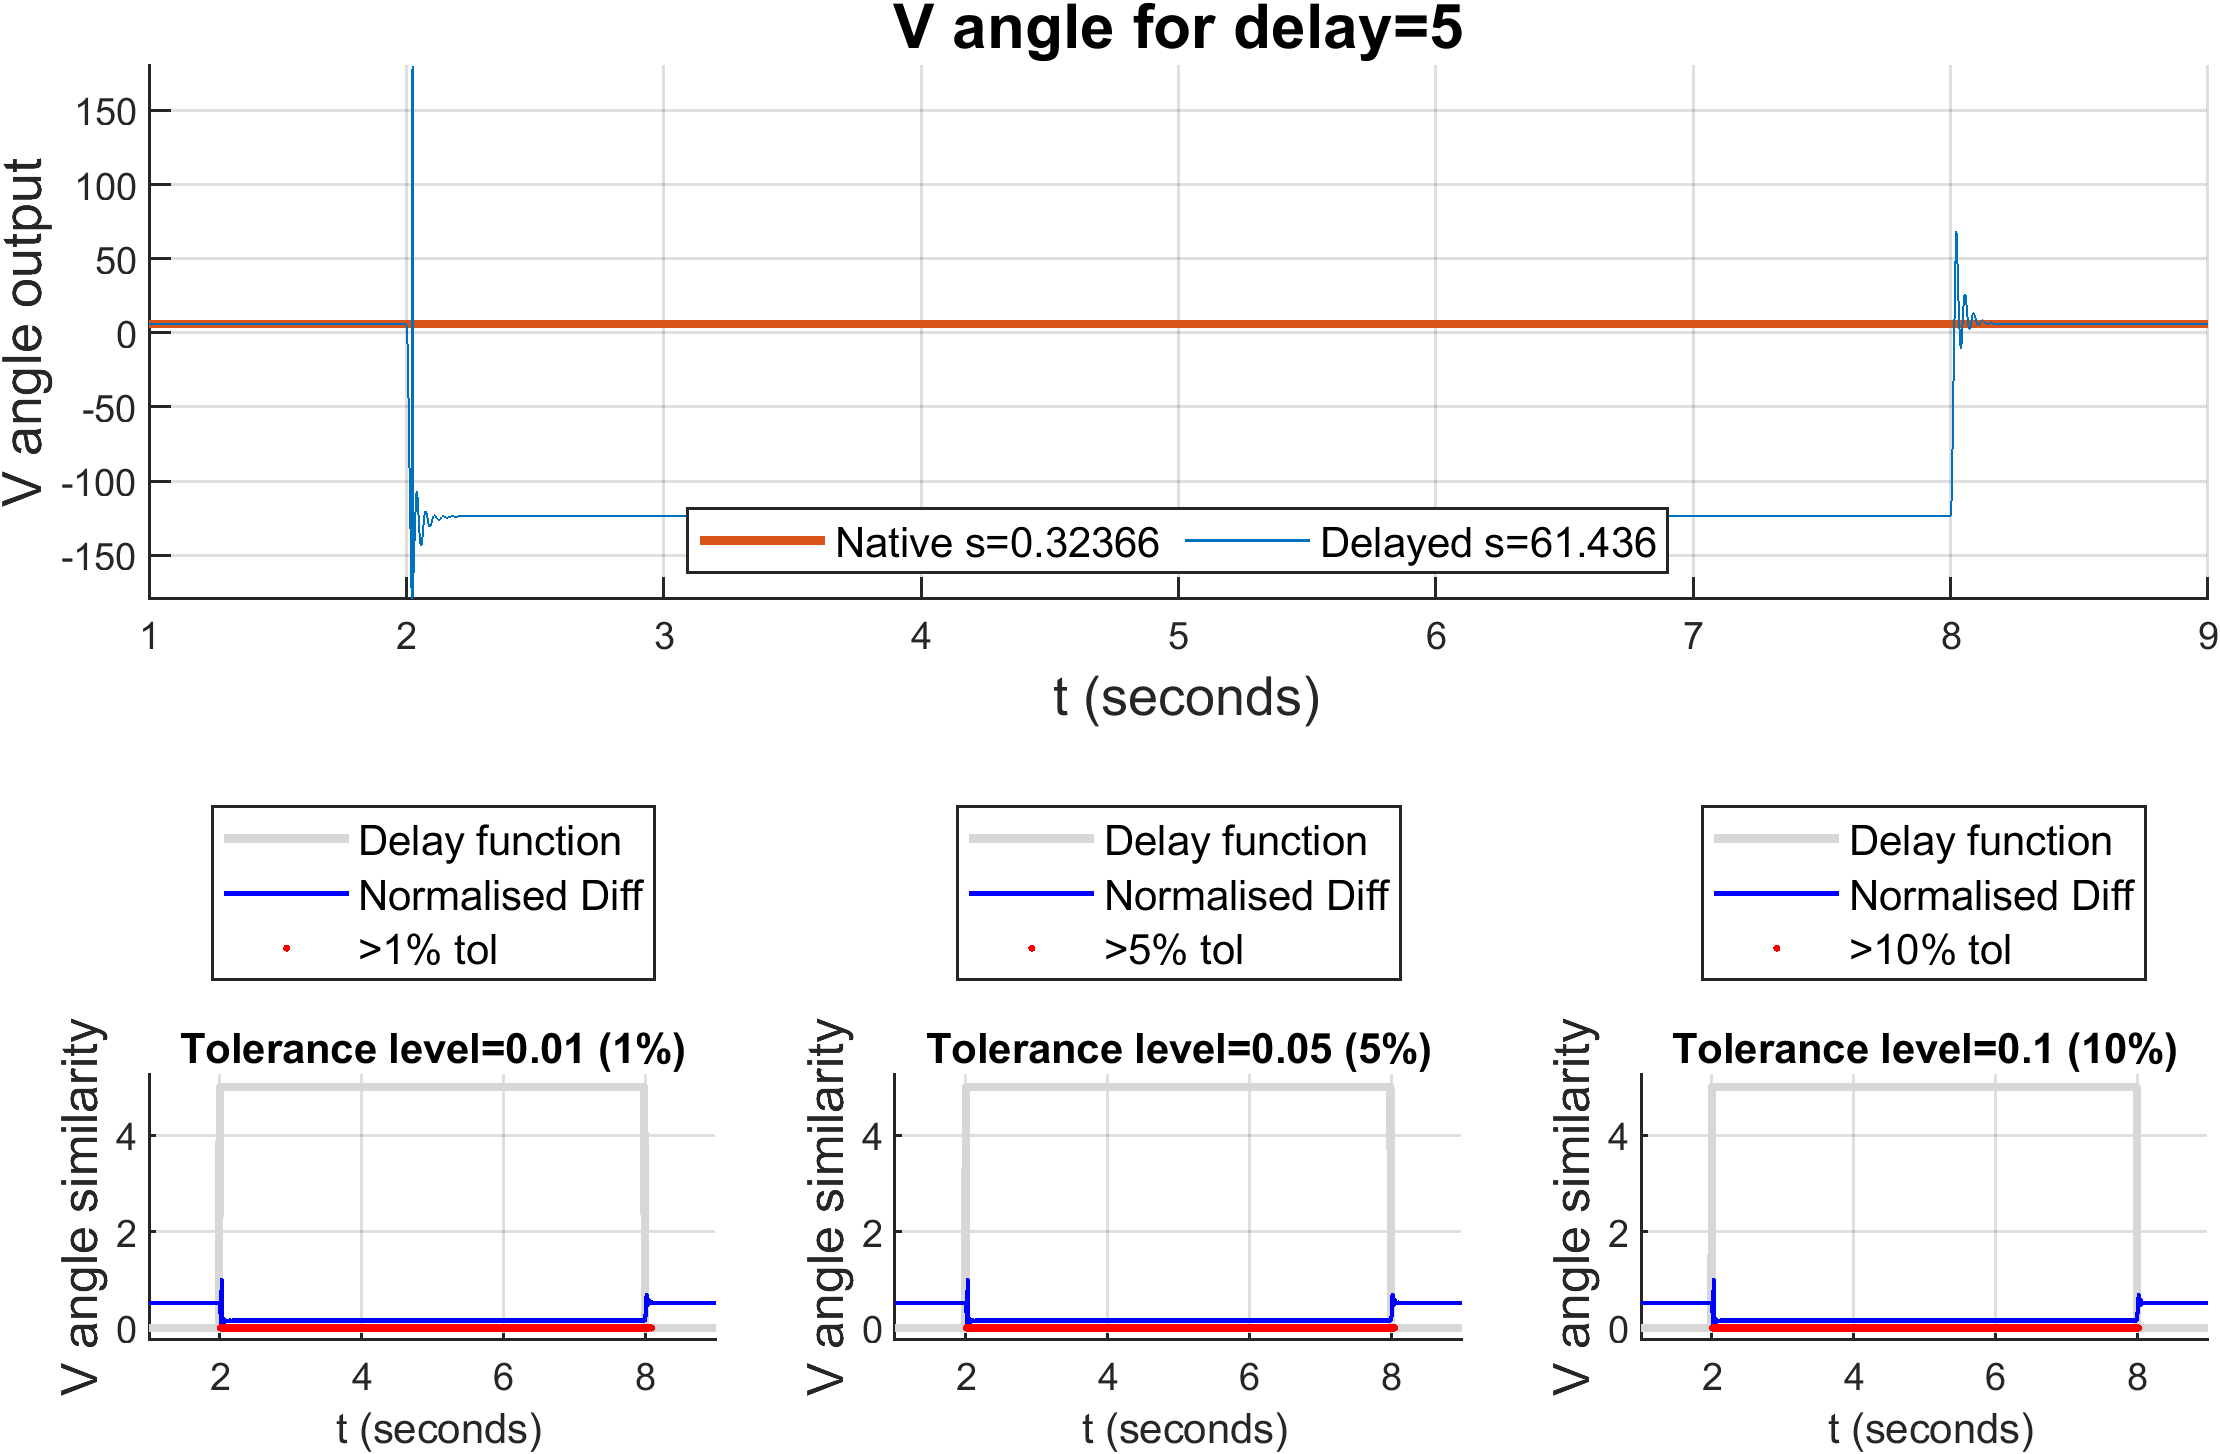
\includegraphics[width=0.95\textwidth]{PMUsim-figures/DelayOf_5/Instant_vAngle.png}} \\   
   \fbox{    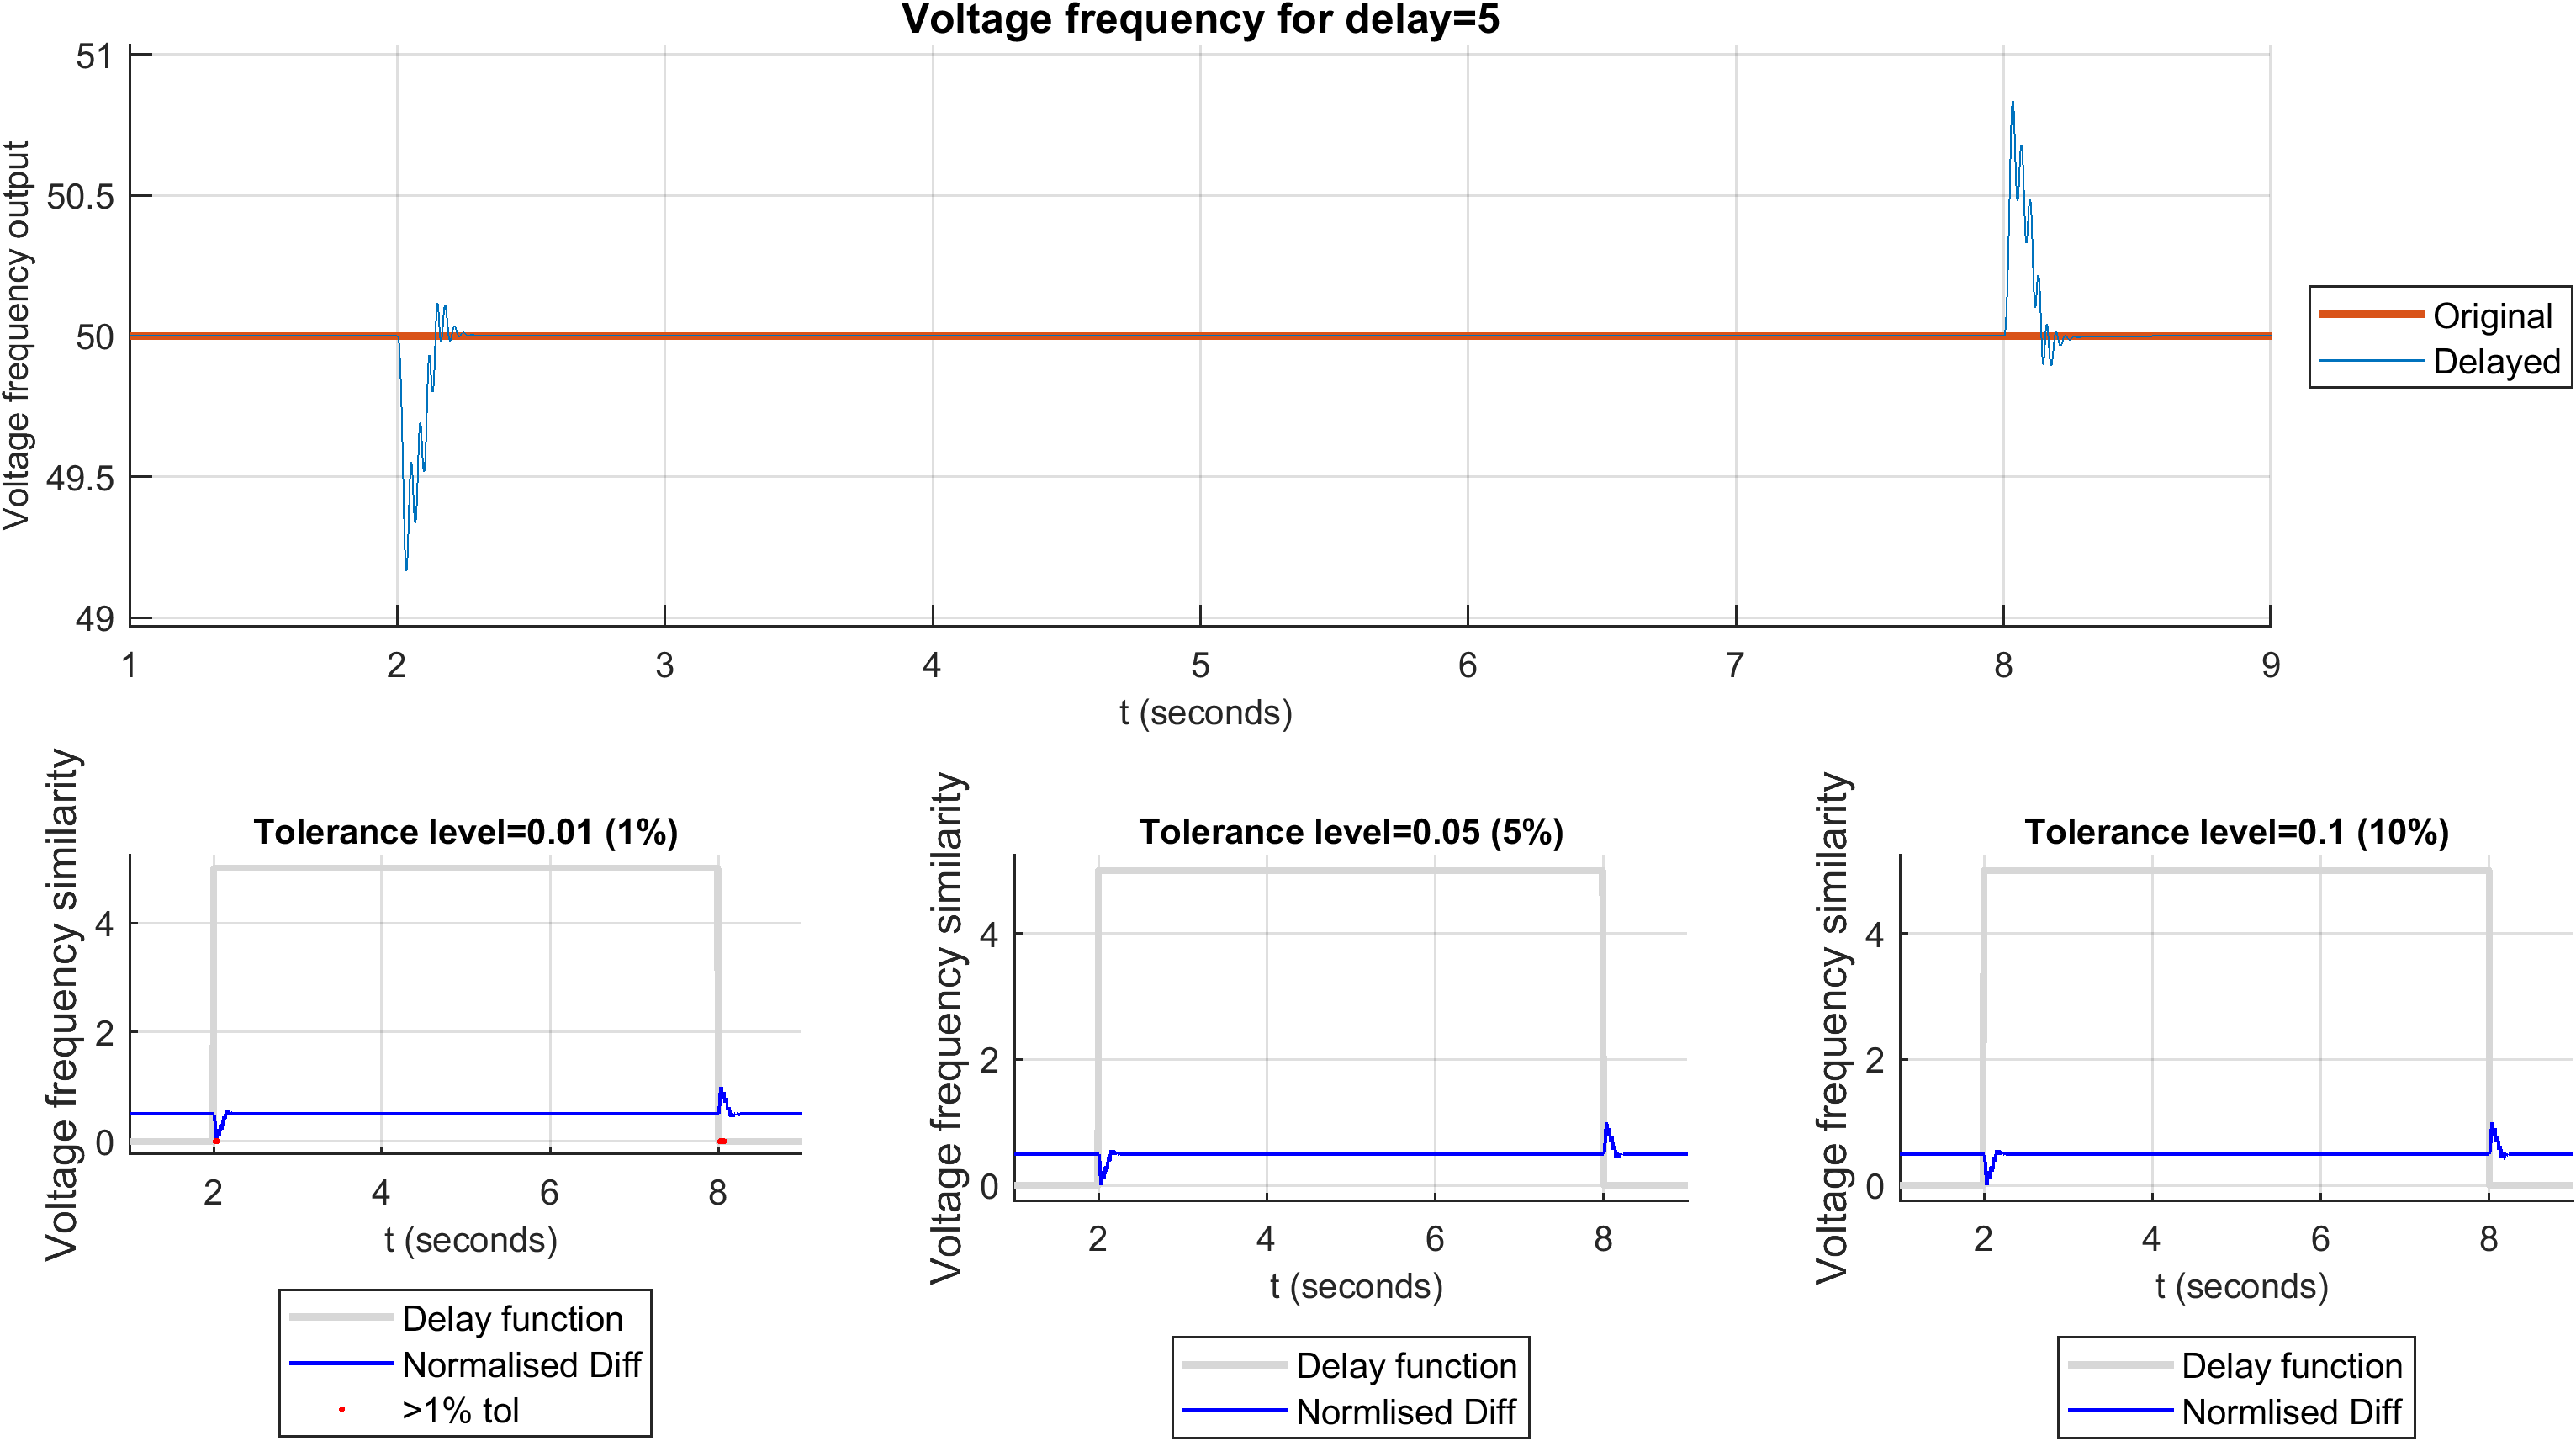
\includegraphics[width=0.95\textwidth]{PMUsim-figures/DelayOf_5/Instant_vFrequency.png}}


  \end{tabular}
\label{fig:VoltageInstantDelayFive}
\caption{Results for Voltage Output for Instant Delay equal to Five }
\end{figure}
\newpage
\begin{figure}[H]
\begin{tabular}{c}
  \fbox{  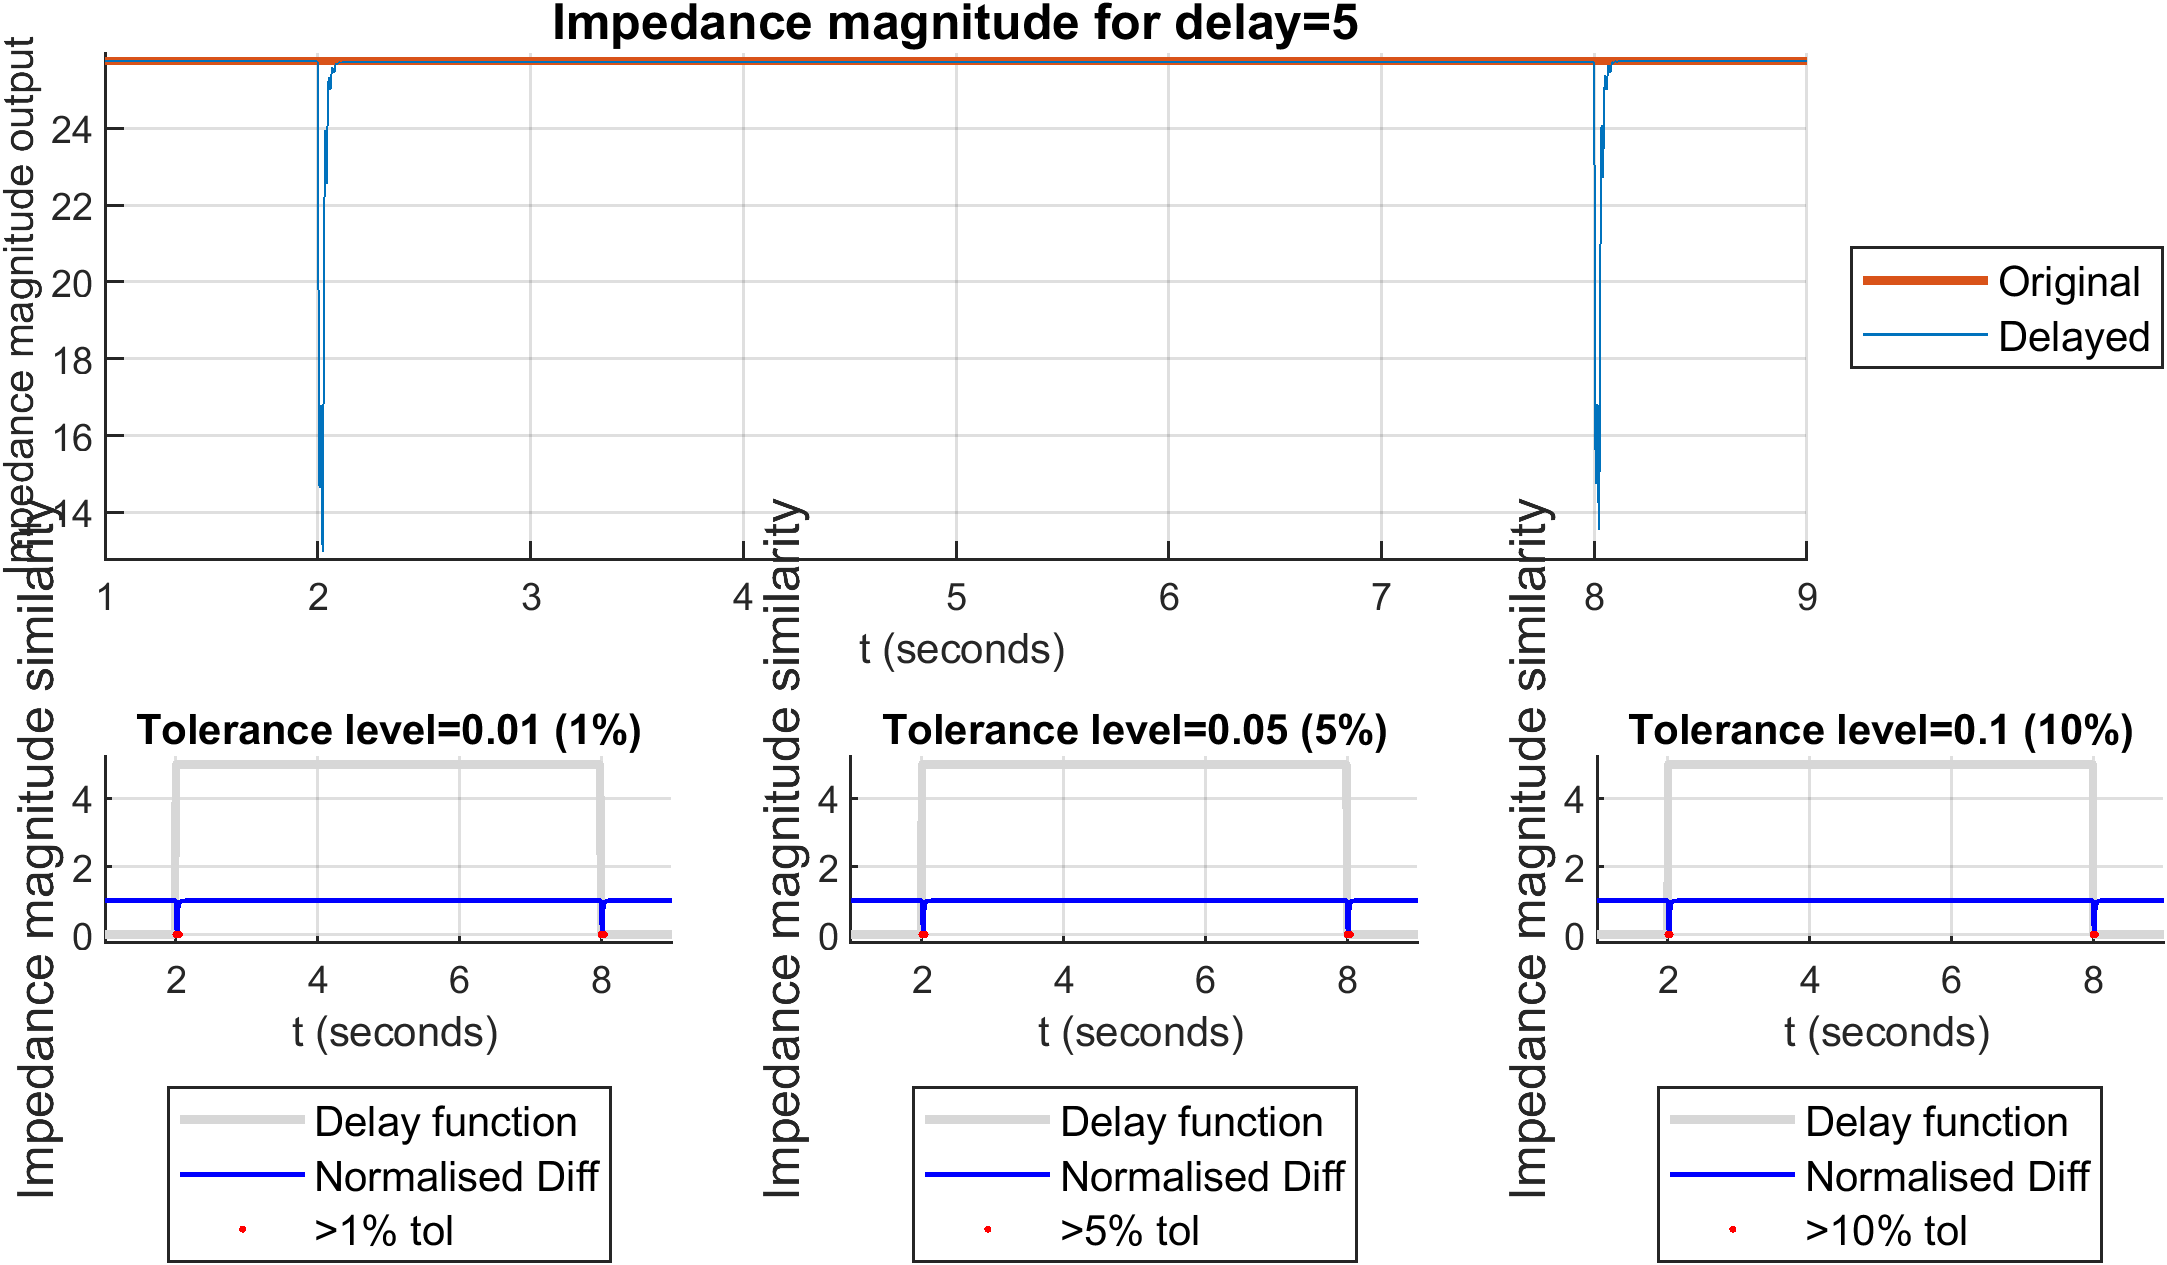
\includegraphics[width=0.95\textwidth]{PMUsim-figures/DelayOf_5/Instant_iMagnitude.png}} \\ 
    \fbox{     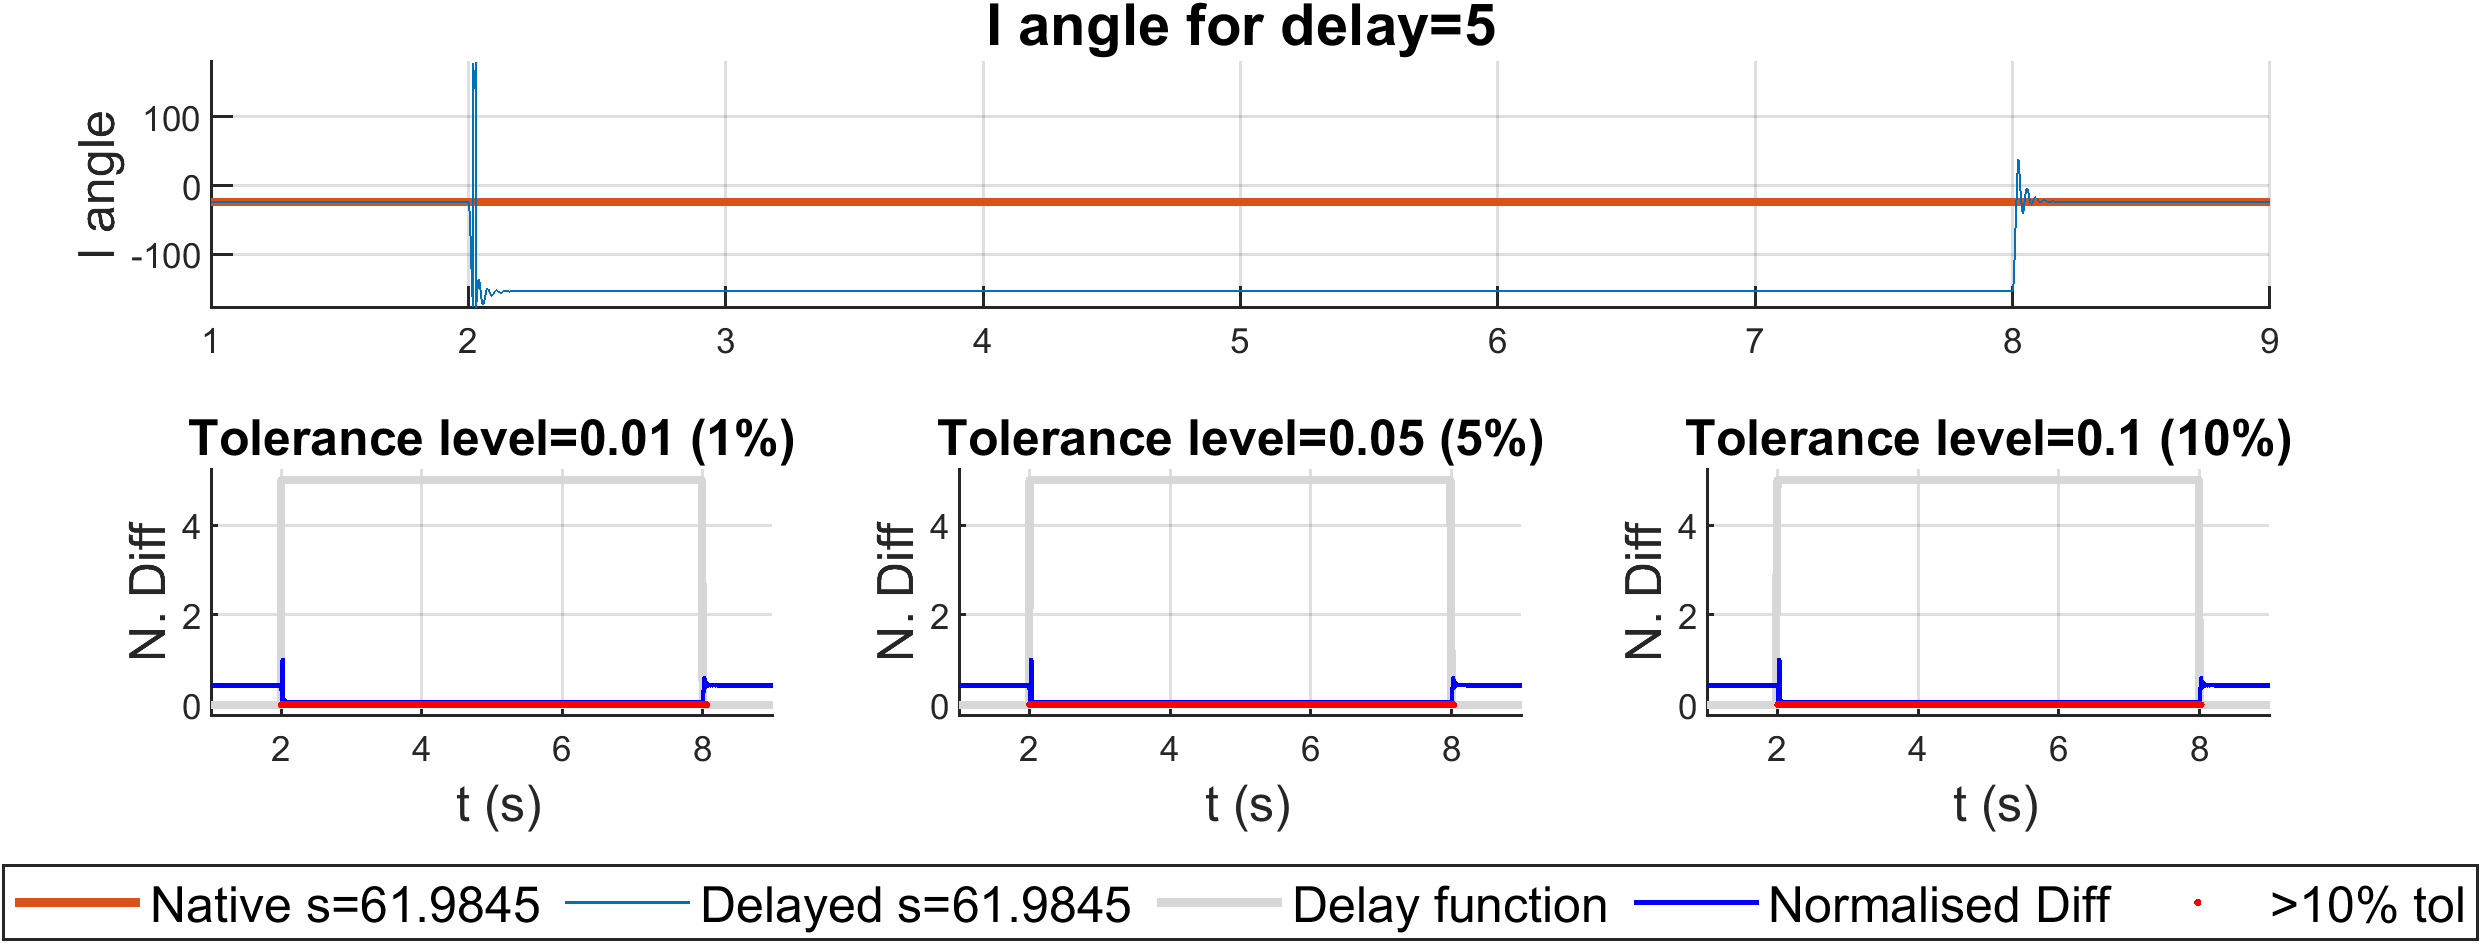
\includegraphics[width=0.95\textwidth]{PMUsim-figures/DelayOf_5/Instant_iAngle.png}} \\  
   \fbox{    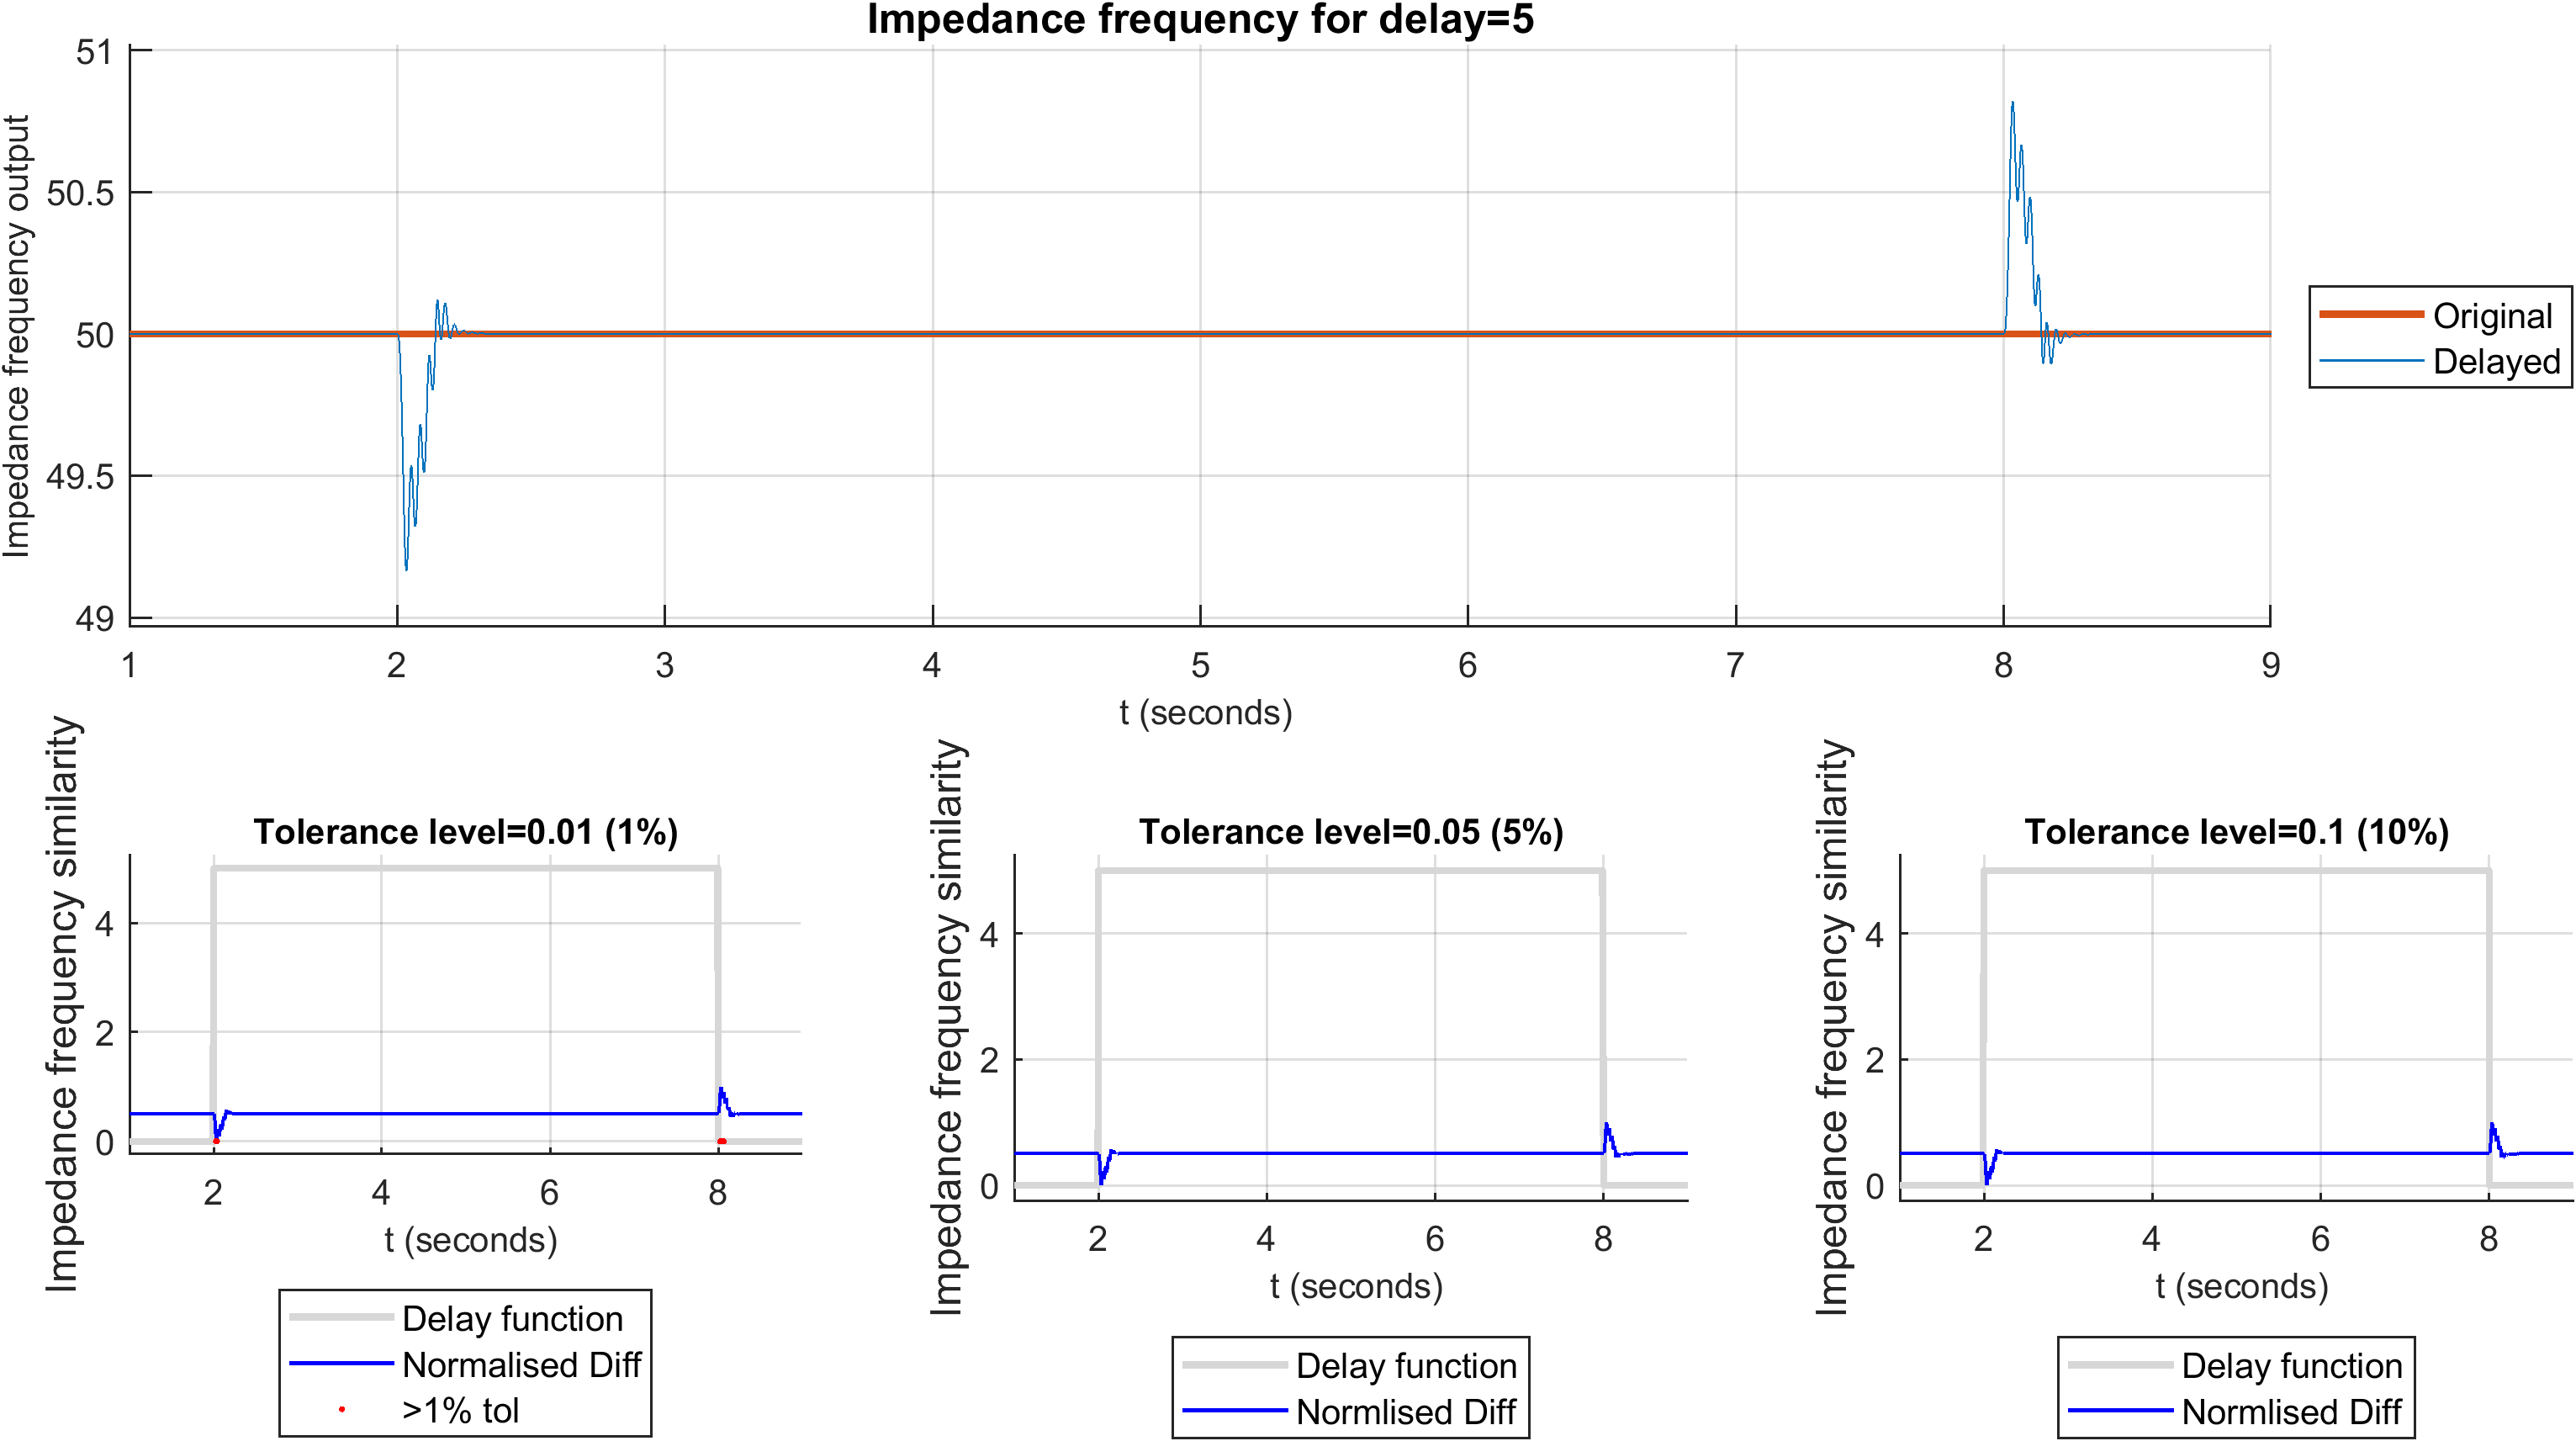
\includegraphics[width=0.95\textwidth]{PMUsim-figures/DelayOf_5/Instant_iFrequency.png}}

 
  \end{tabular}
\label{fig:ImpedanceInstantDelayFive}
\caption{Results for Impedance Output for Instant Delay equal to Five }
\end{figure}


\newpage
\begin{figure}[H]
\begin{tabular}{c}
  \fbox{  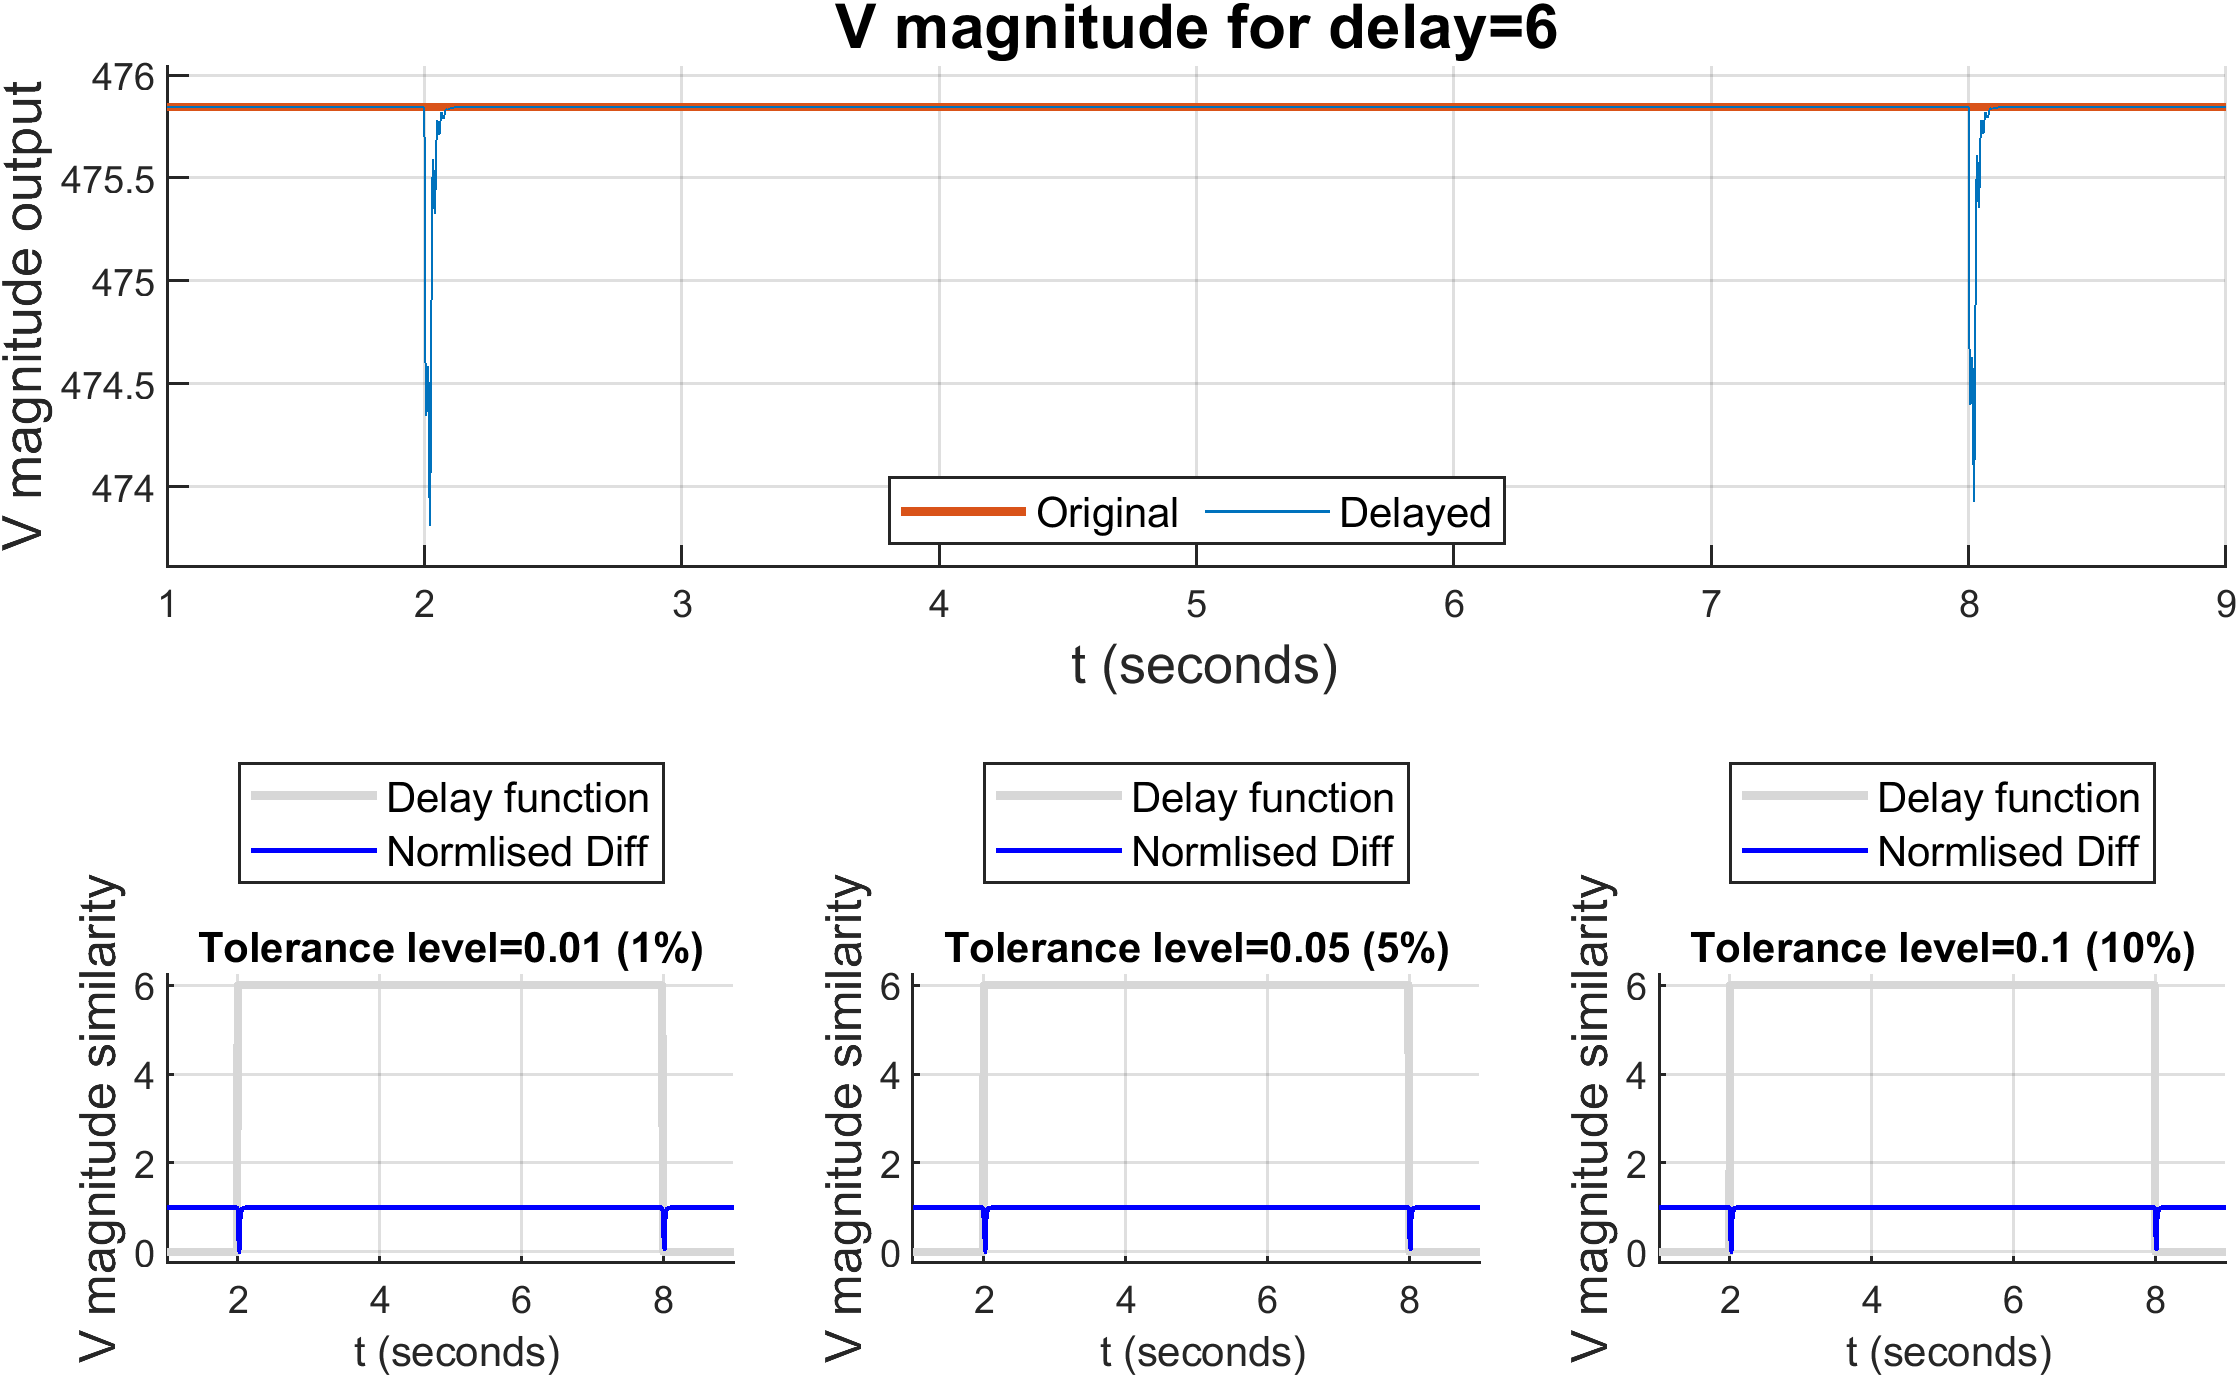
\includegraphics[width=0.95\textwidth]{PMUsim-figures/DelayOf_6/Instant_vMagnitude.png}} \\ 
   \fbox{     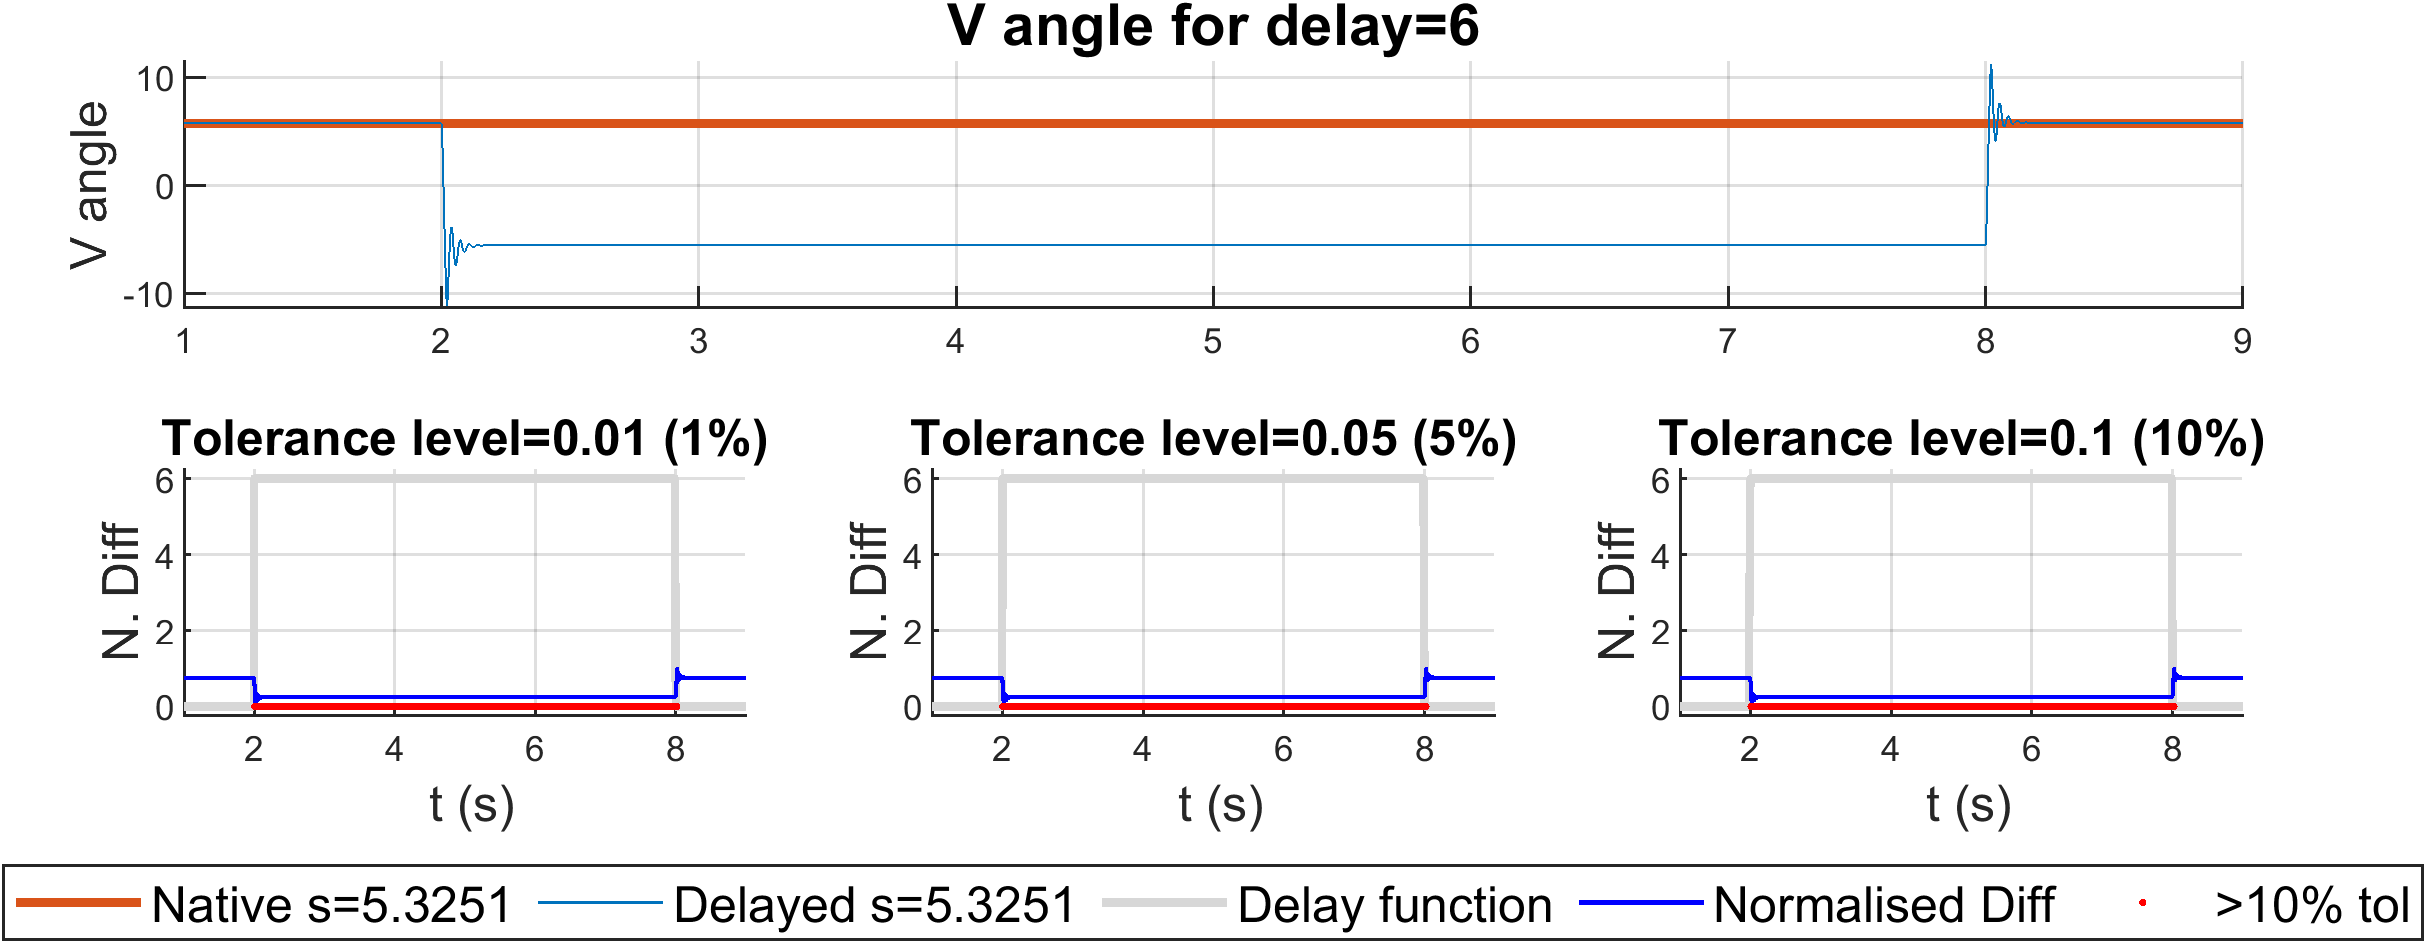
\includegraphics[width=0.95\textwidth]{PMUsim-figures/DelayOf_6/Instant_vAngle.png}} \\   
   \fbox{    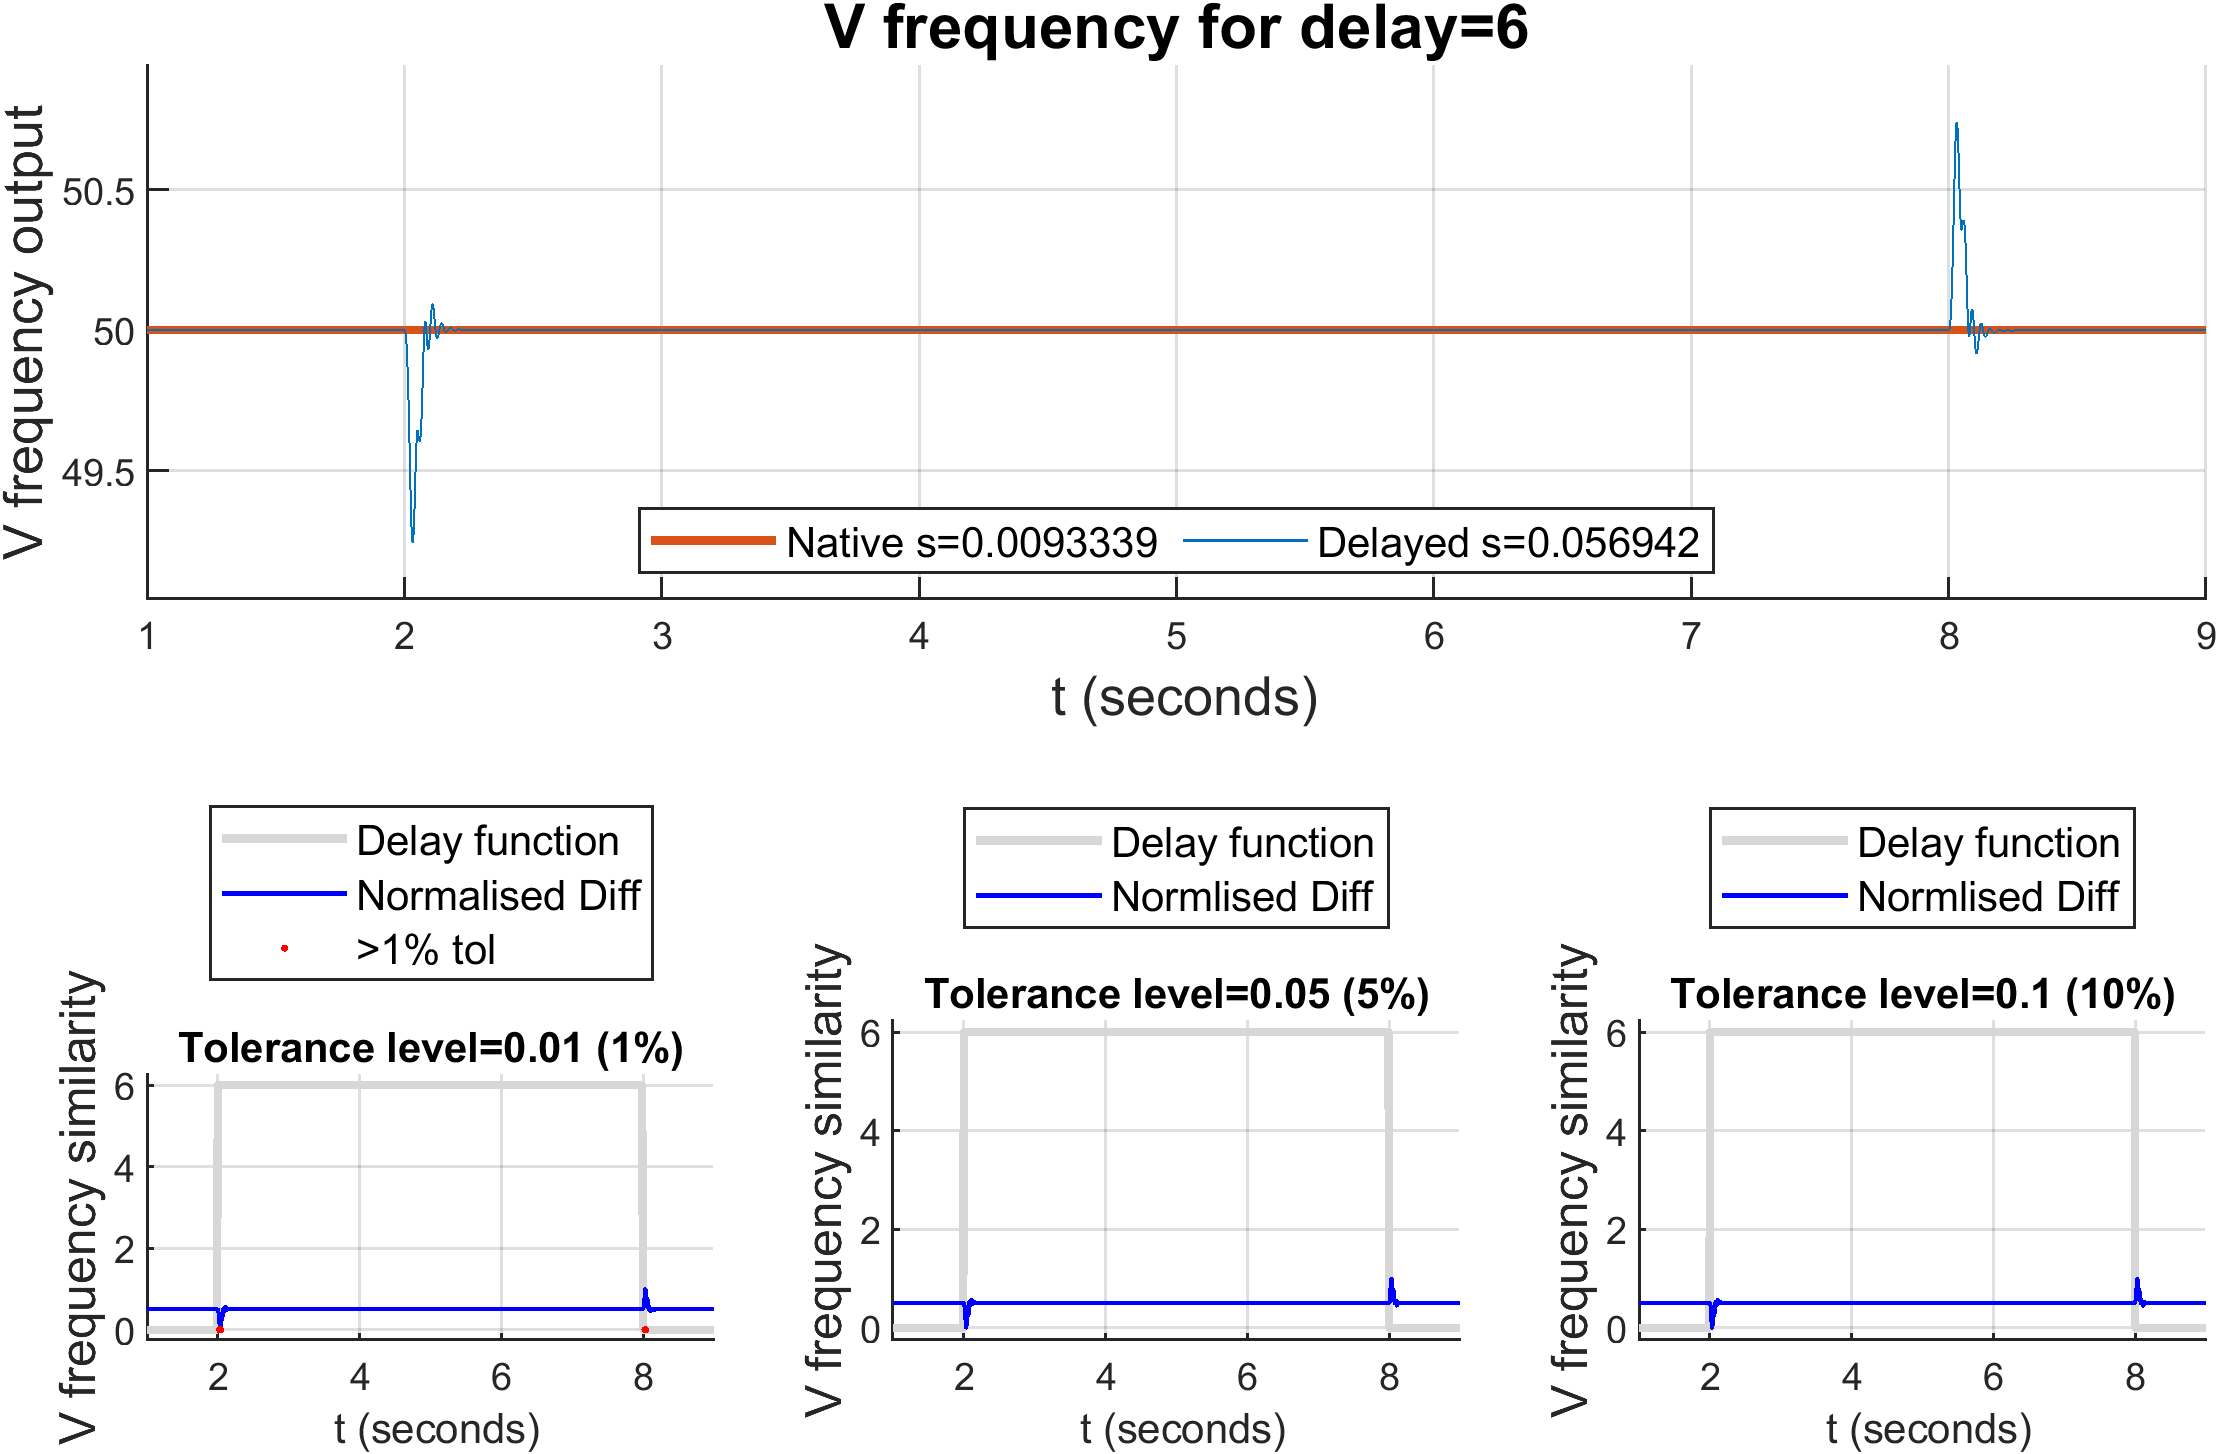
\includegraphics[width=0.95\textwidth]{PMUsim-figures/DelayOf_6/Instant_vFrequency.png}}

 
  \end{tabular}
\label{fig:VoltageInstantDelaySix}
\caption{Results for Voltage Output for Instant Delay equal to Six }
\end{figure}
\newpage
\begin{figure}[H]
\begin{tabular}{c}
  \fbox{  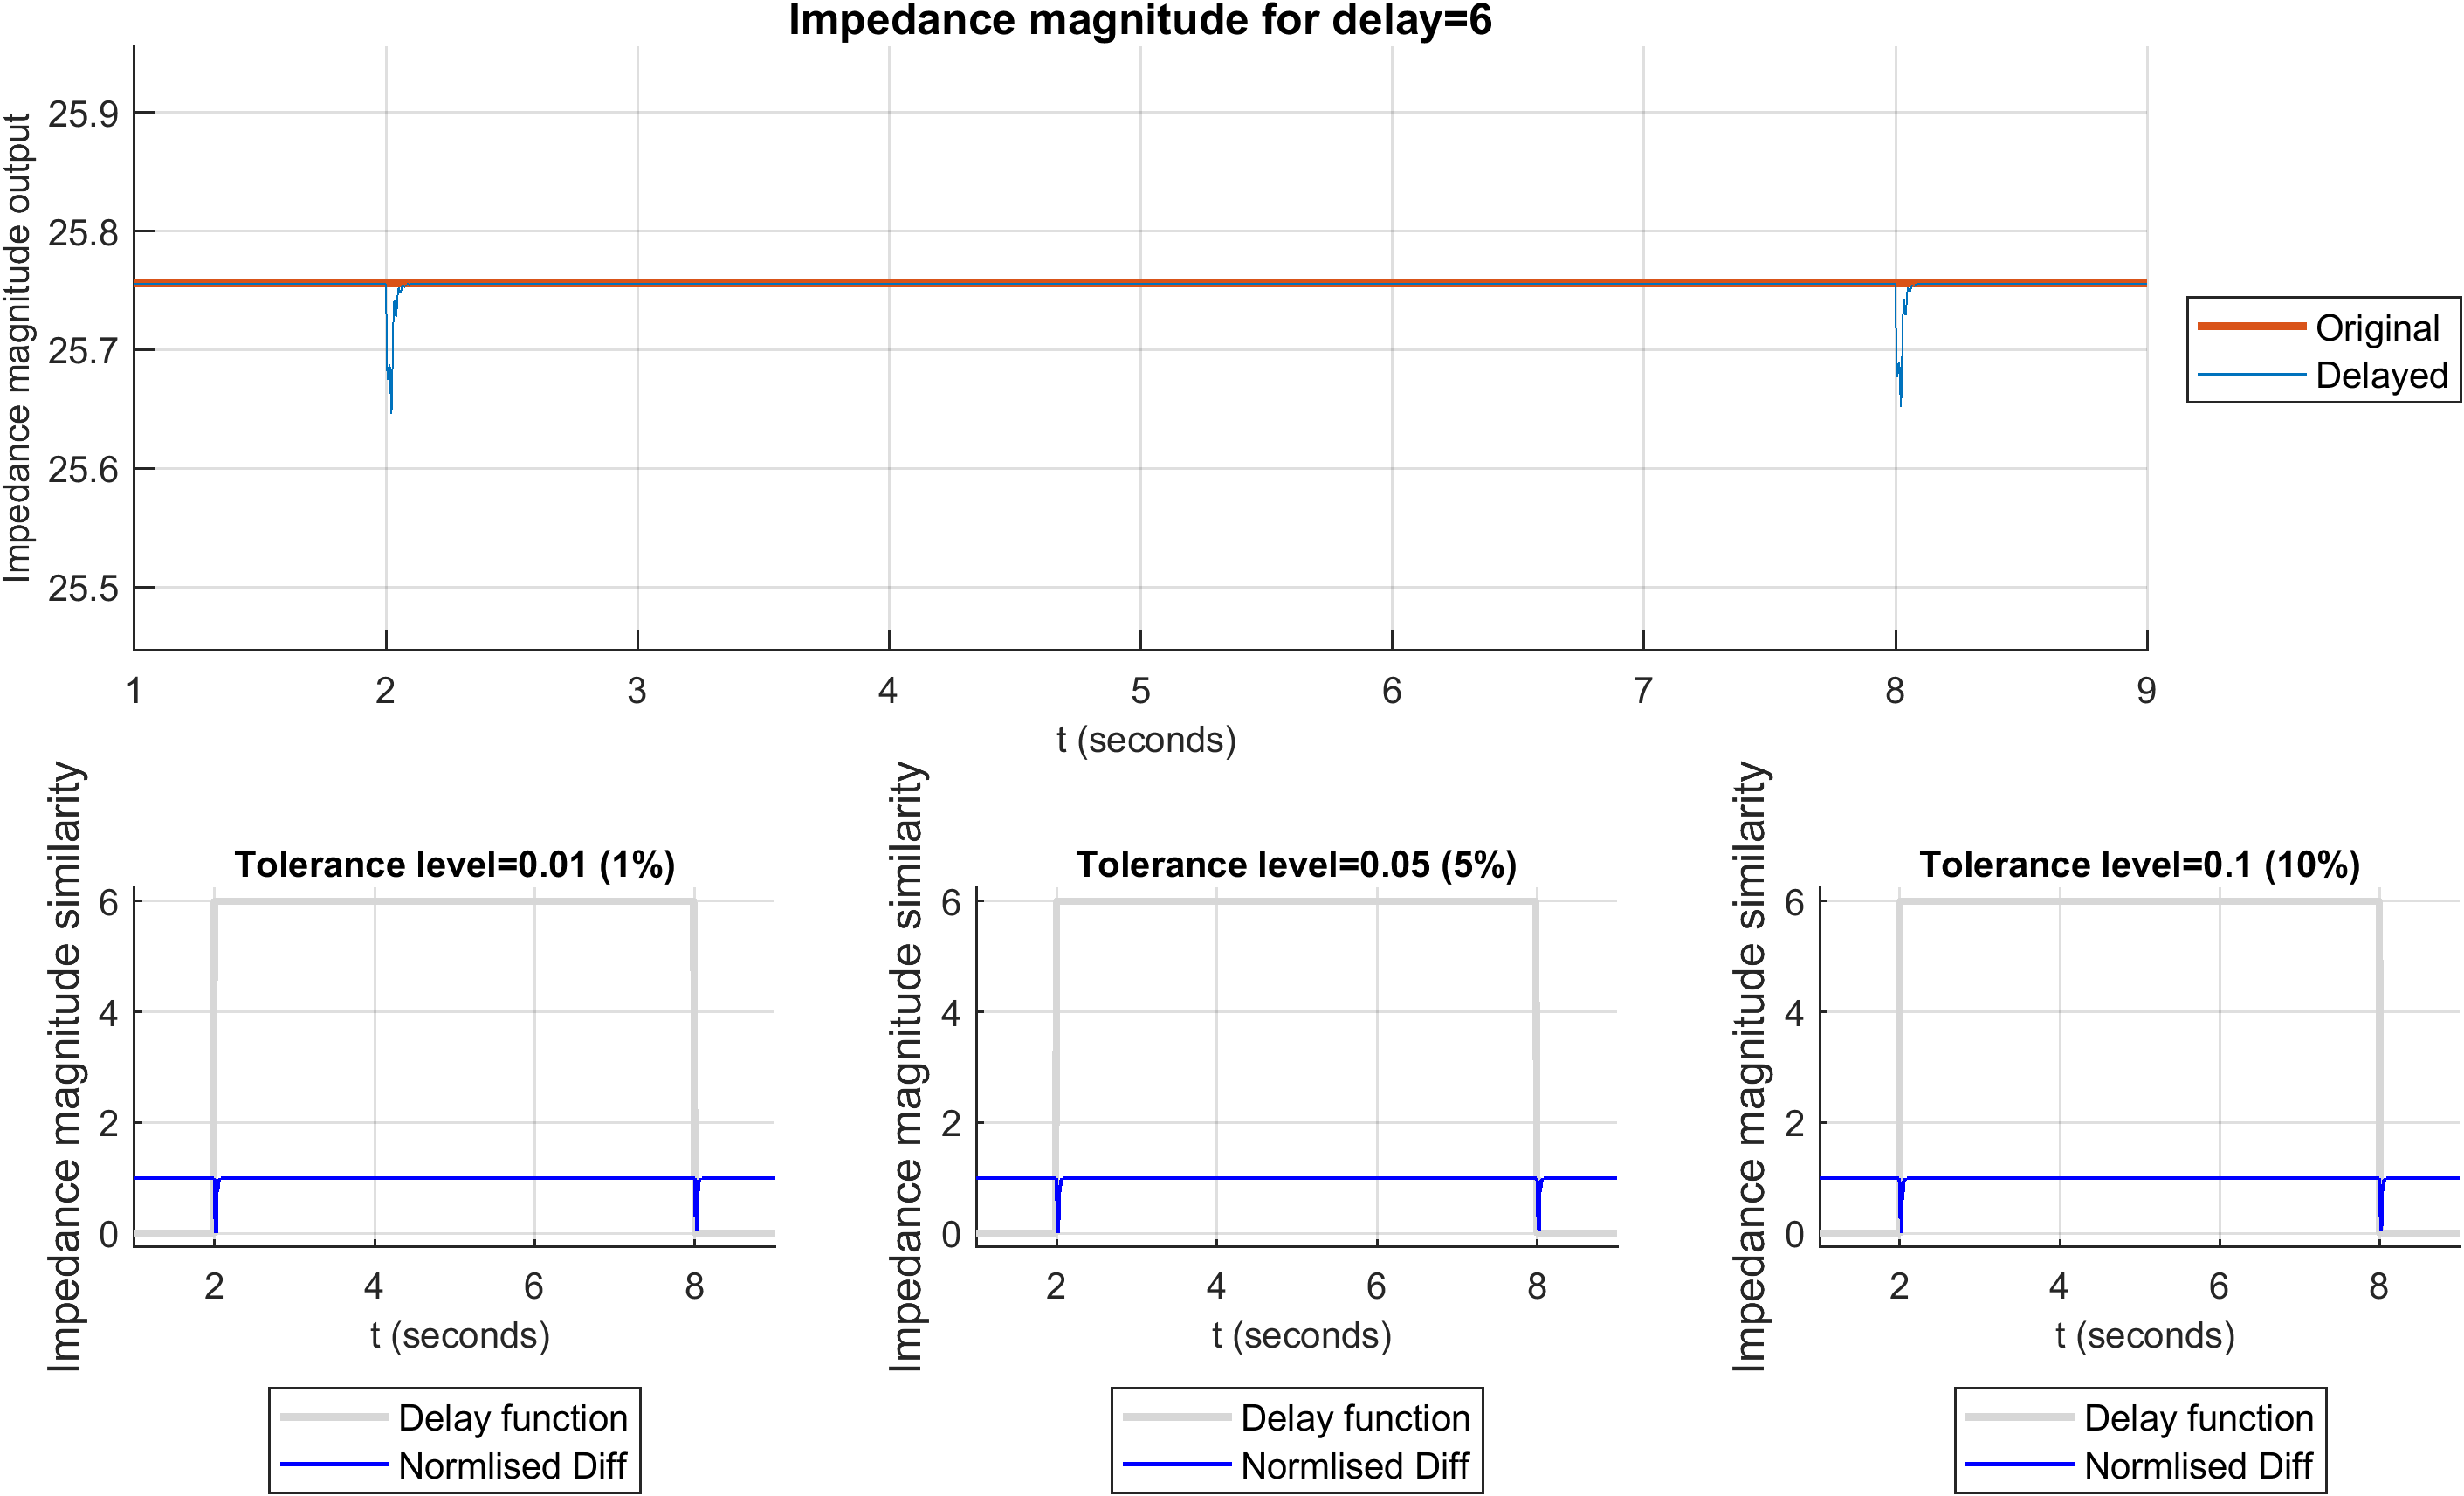
\includegraphics[width=0.95\textwidth]{PMUsim-figures/DelayOf_6/Instant_iMagnitude.png}} \\ 
   \fbox{     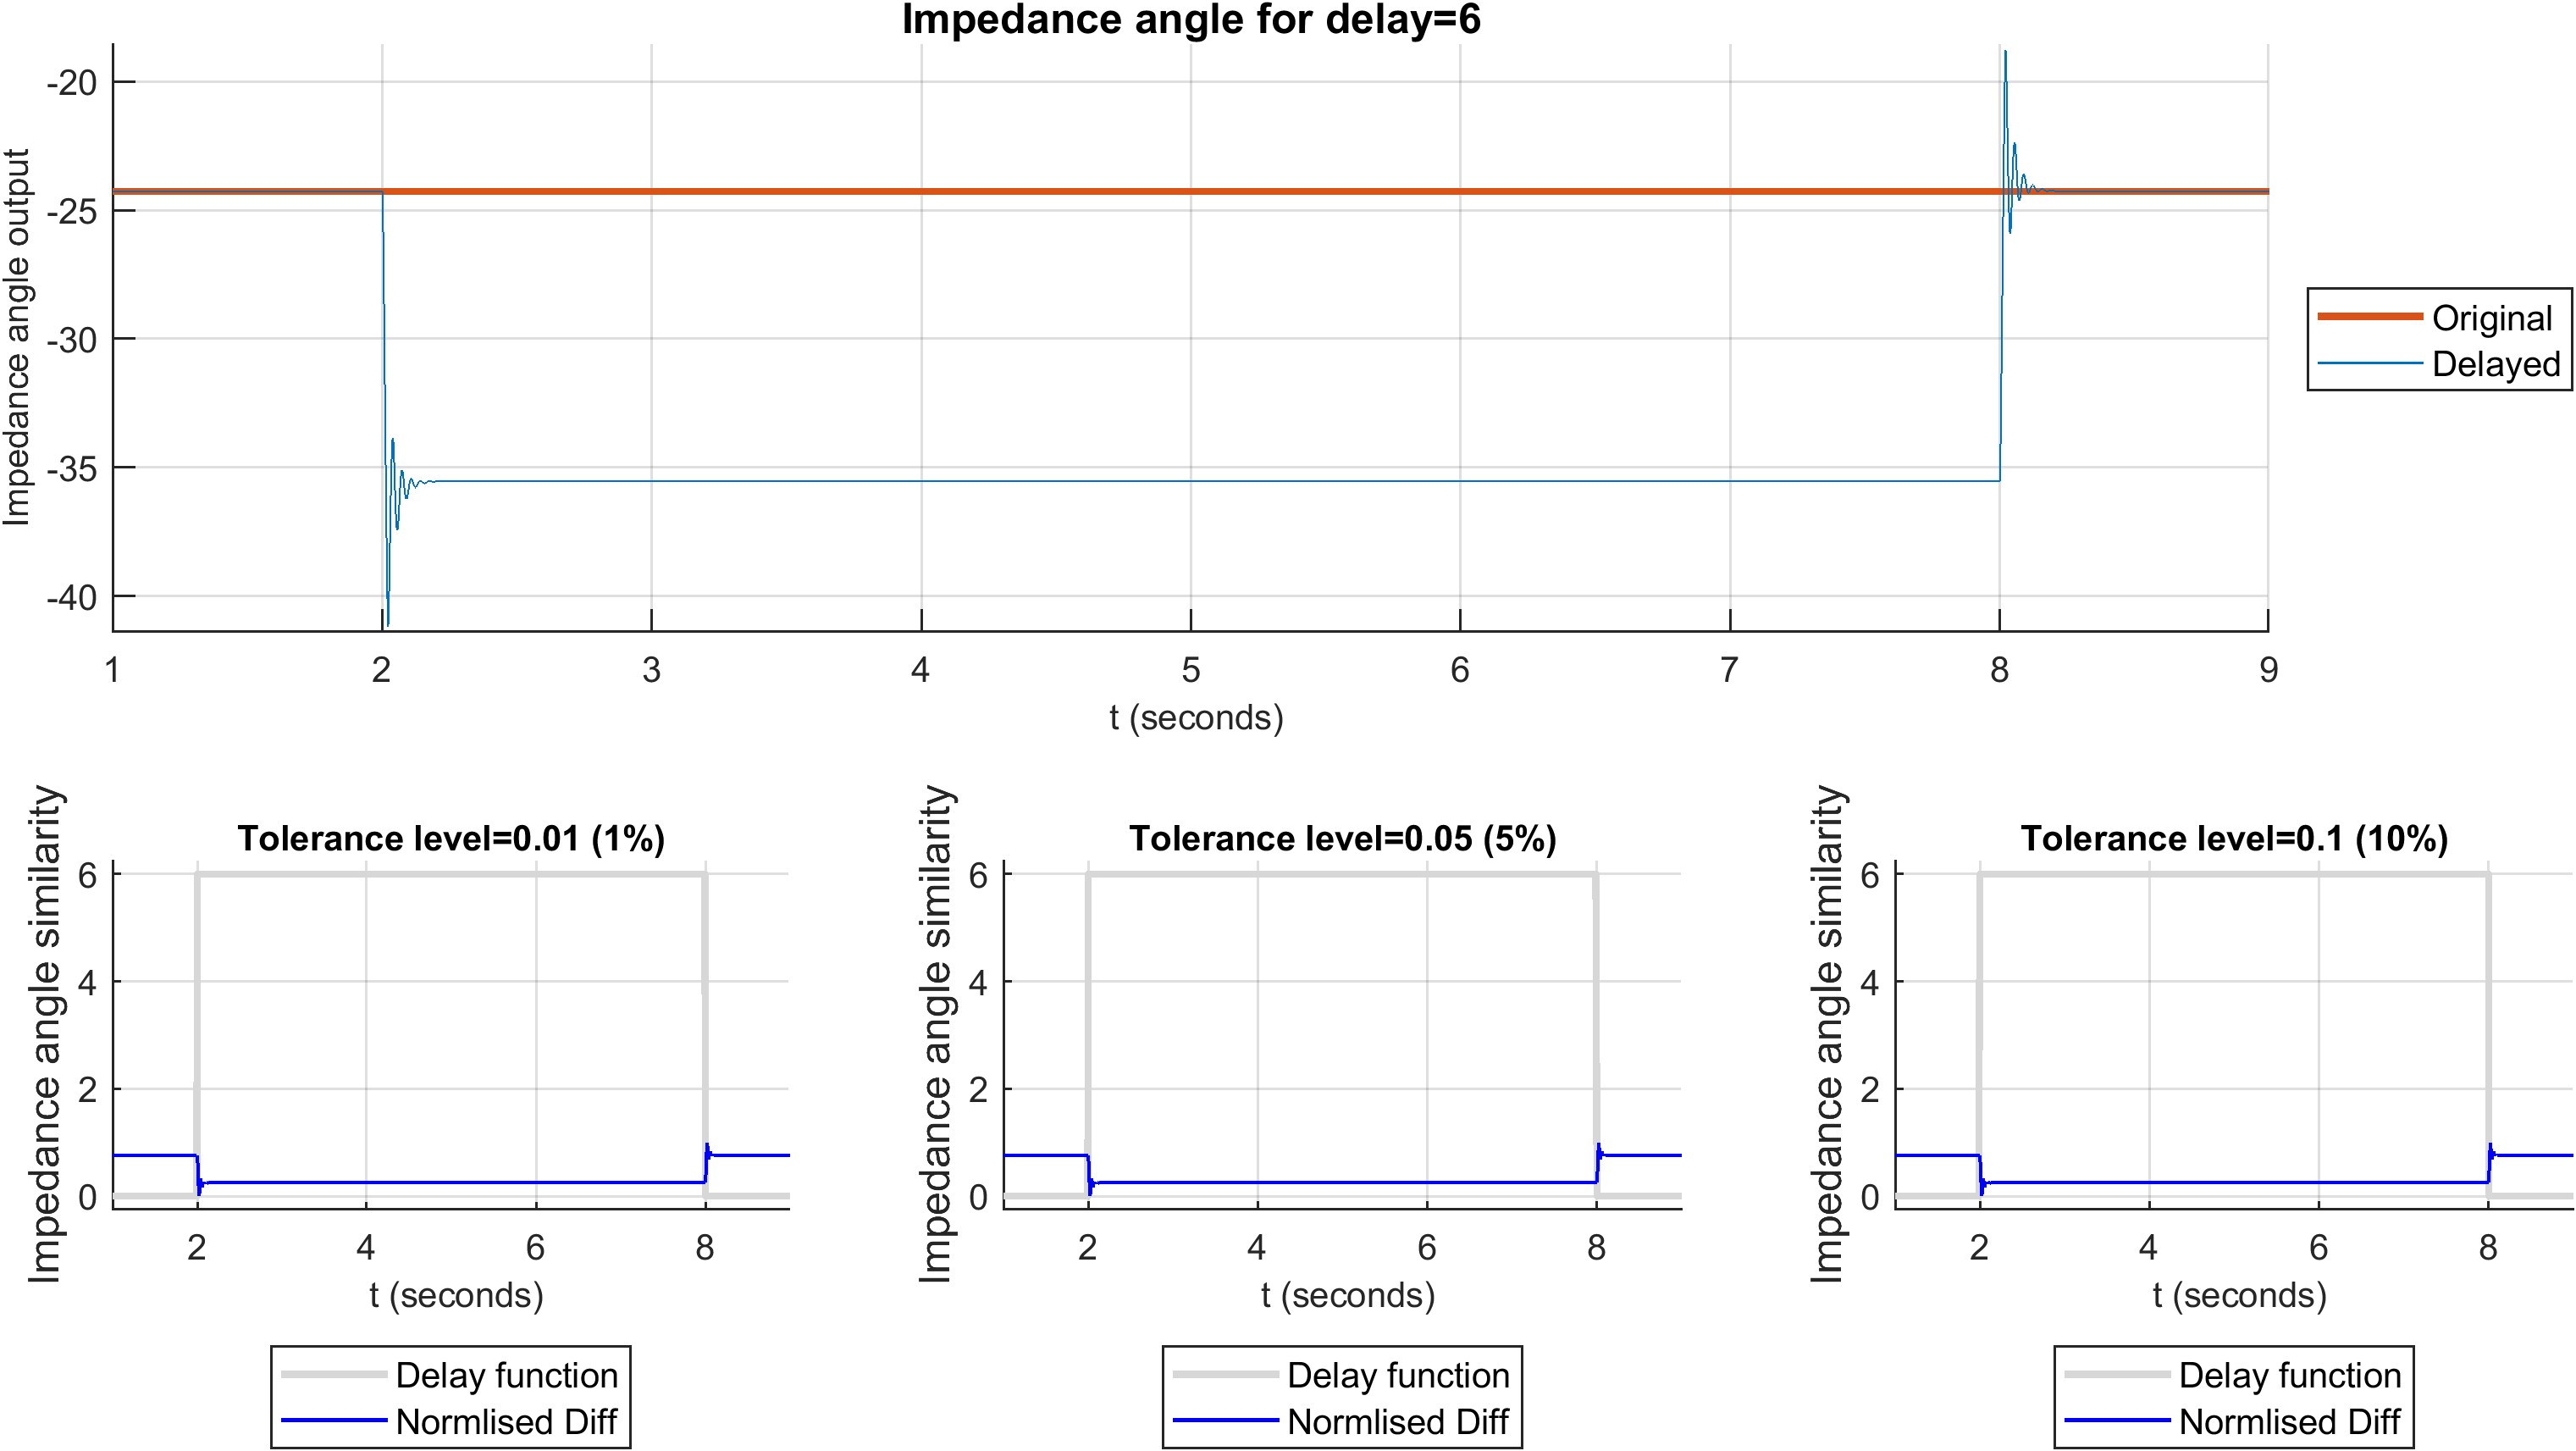
\includegraphics[width=0.95\textwidth]{PMUsim-figures/DelayOf_6/Instant_iAngle.png}} \\   
   \fbox{    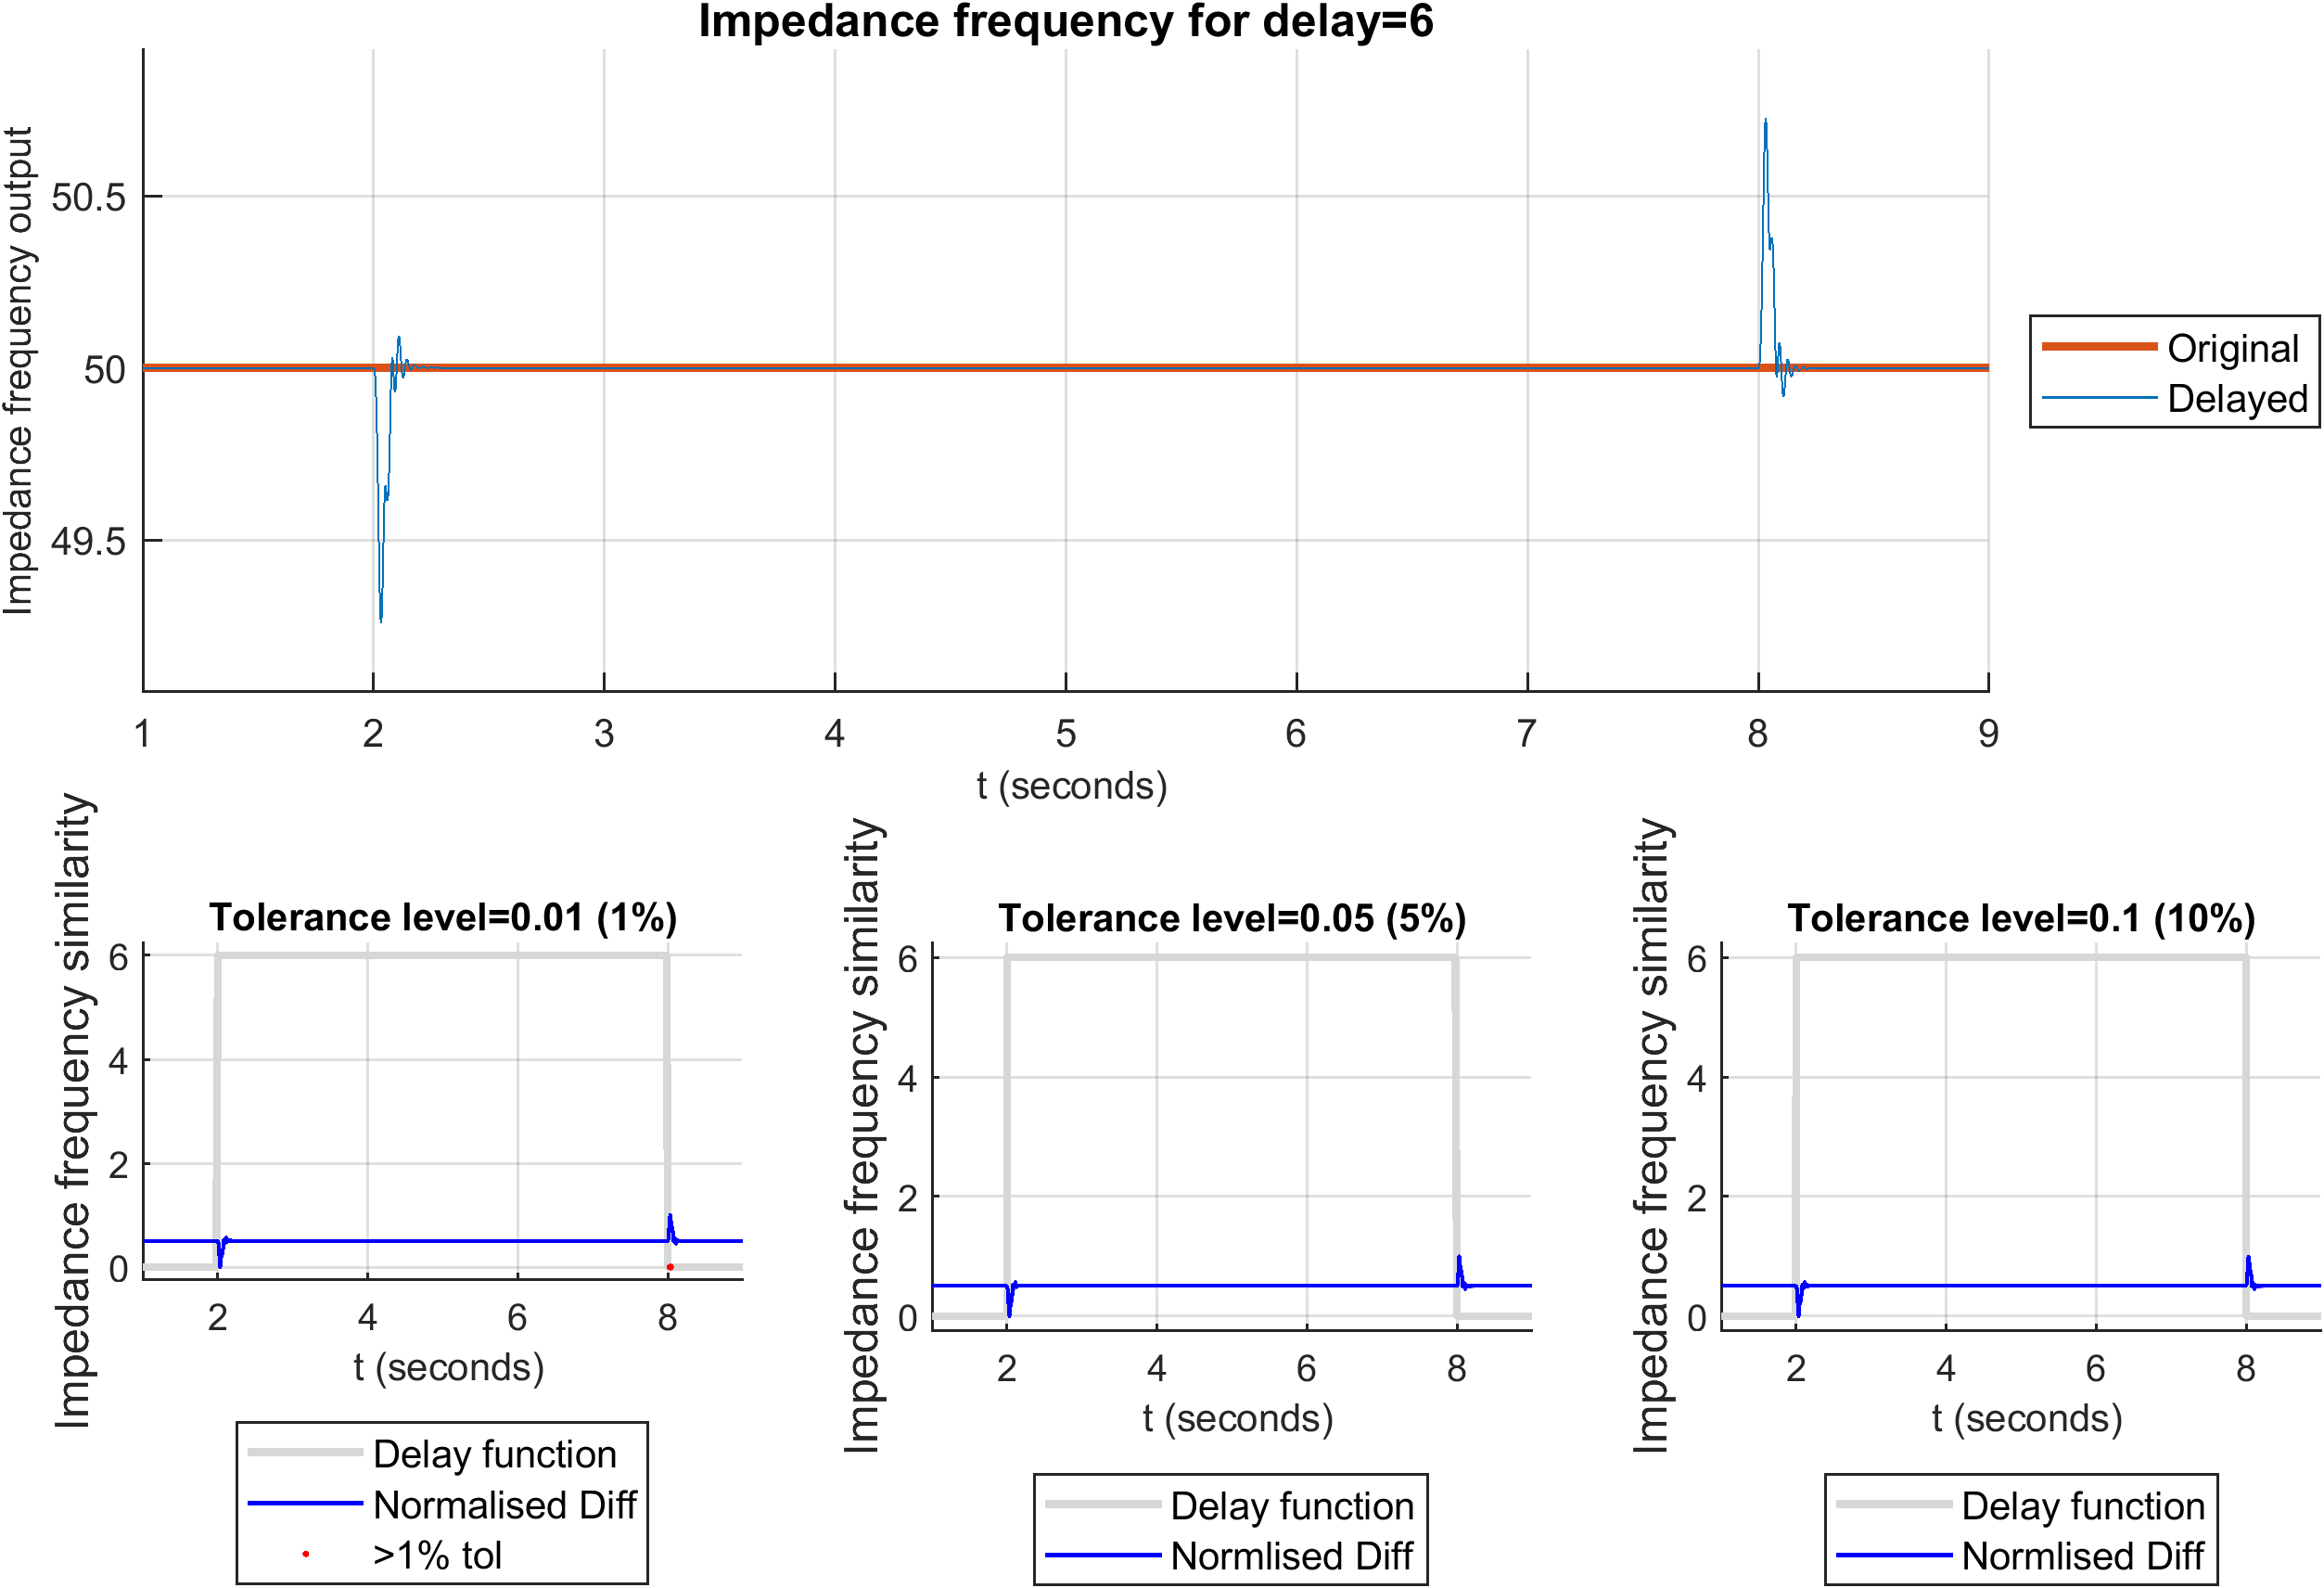
\includegraphics[width=0.95\textwidth]{PMUsim-figures/DelayOf_6/Instant_iFrequency.png}}

 
  \end{tabular}
\label{fig:ImpedanceInstantDelaySix}
\caption{Results for Impedance Output for Instant Delay equal to Six }
\end{figure}



























\newpage
\begin{figure}[H]
\begin{tabular}{c}
  \fbox{  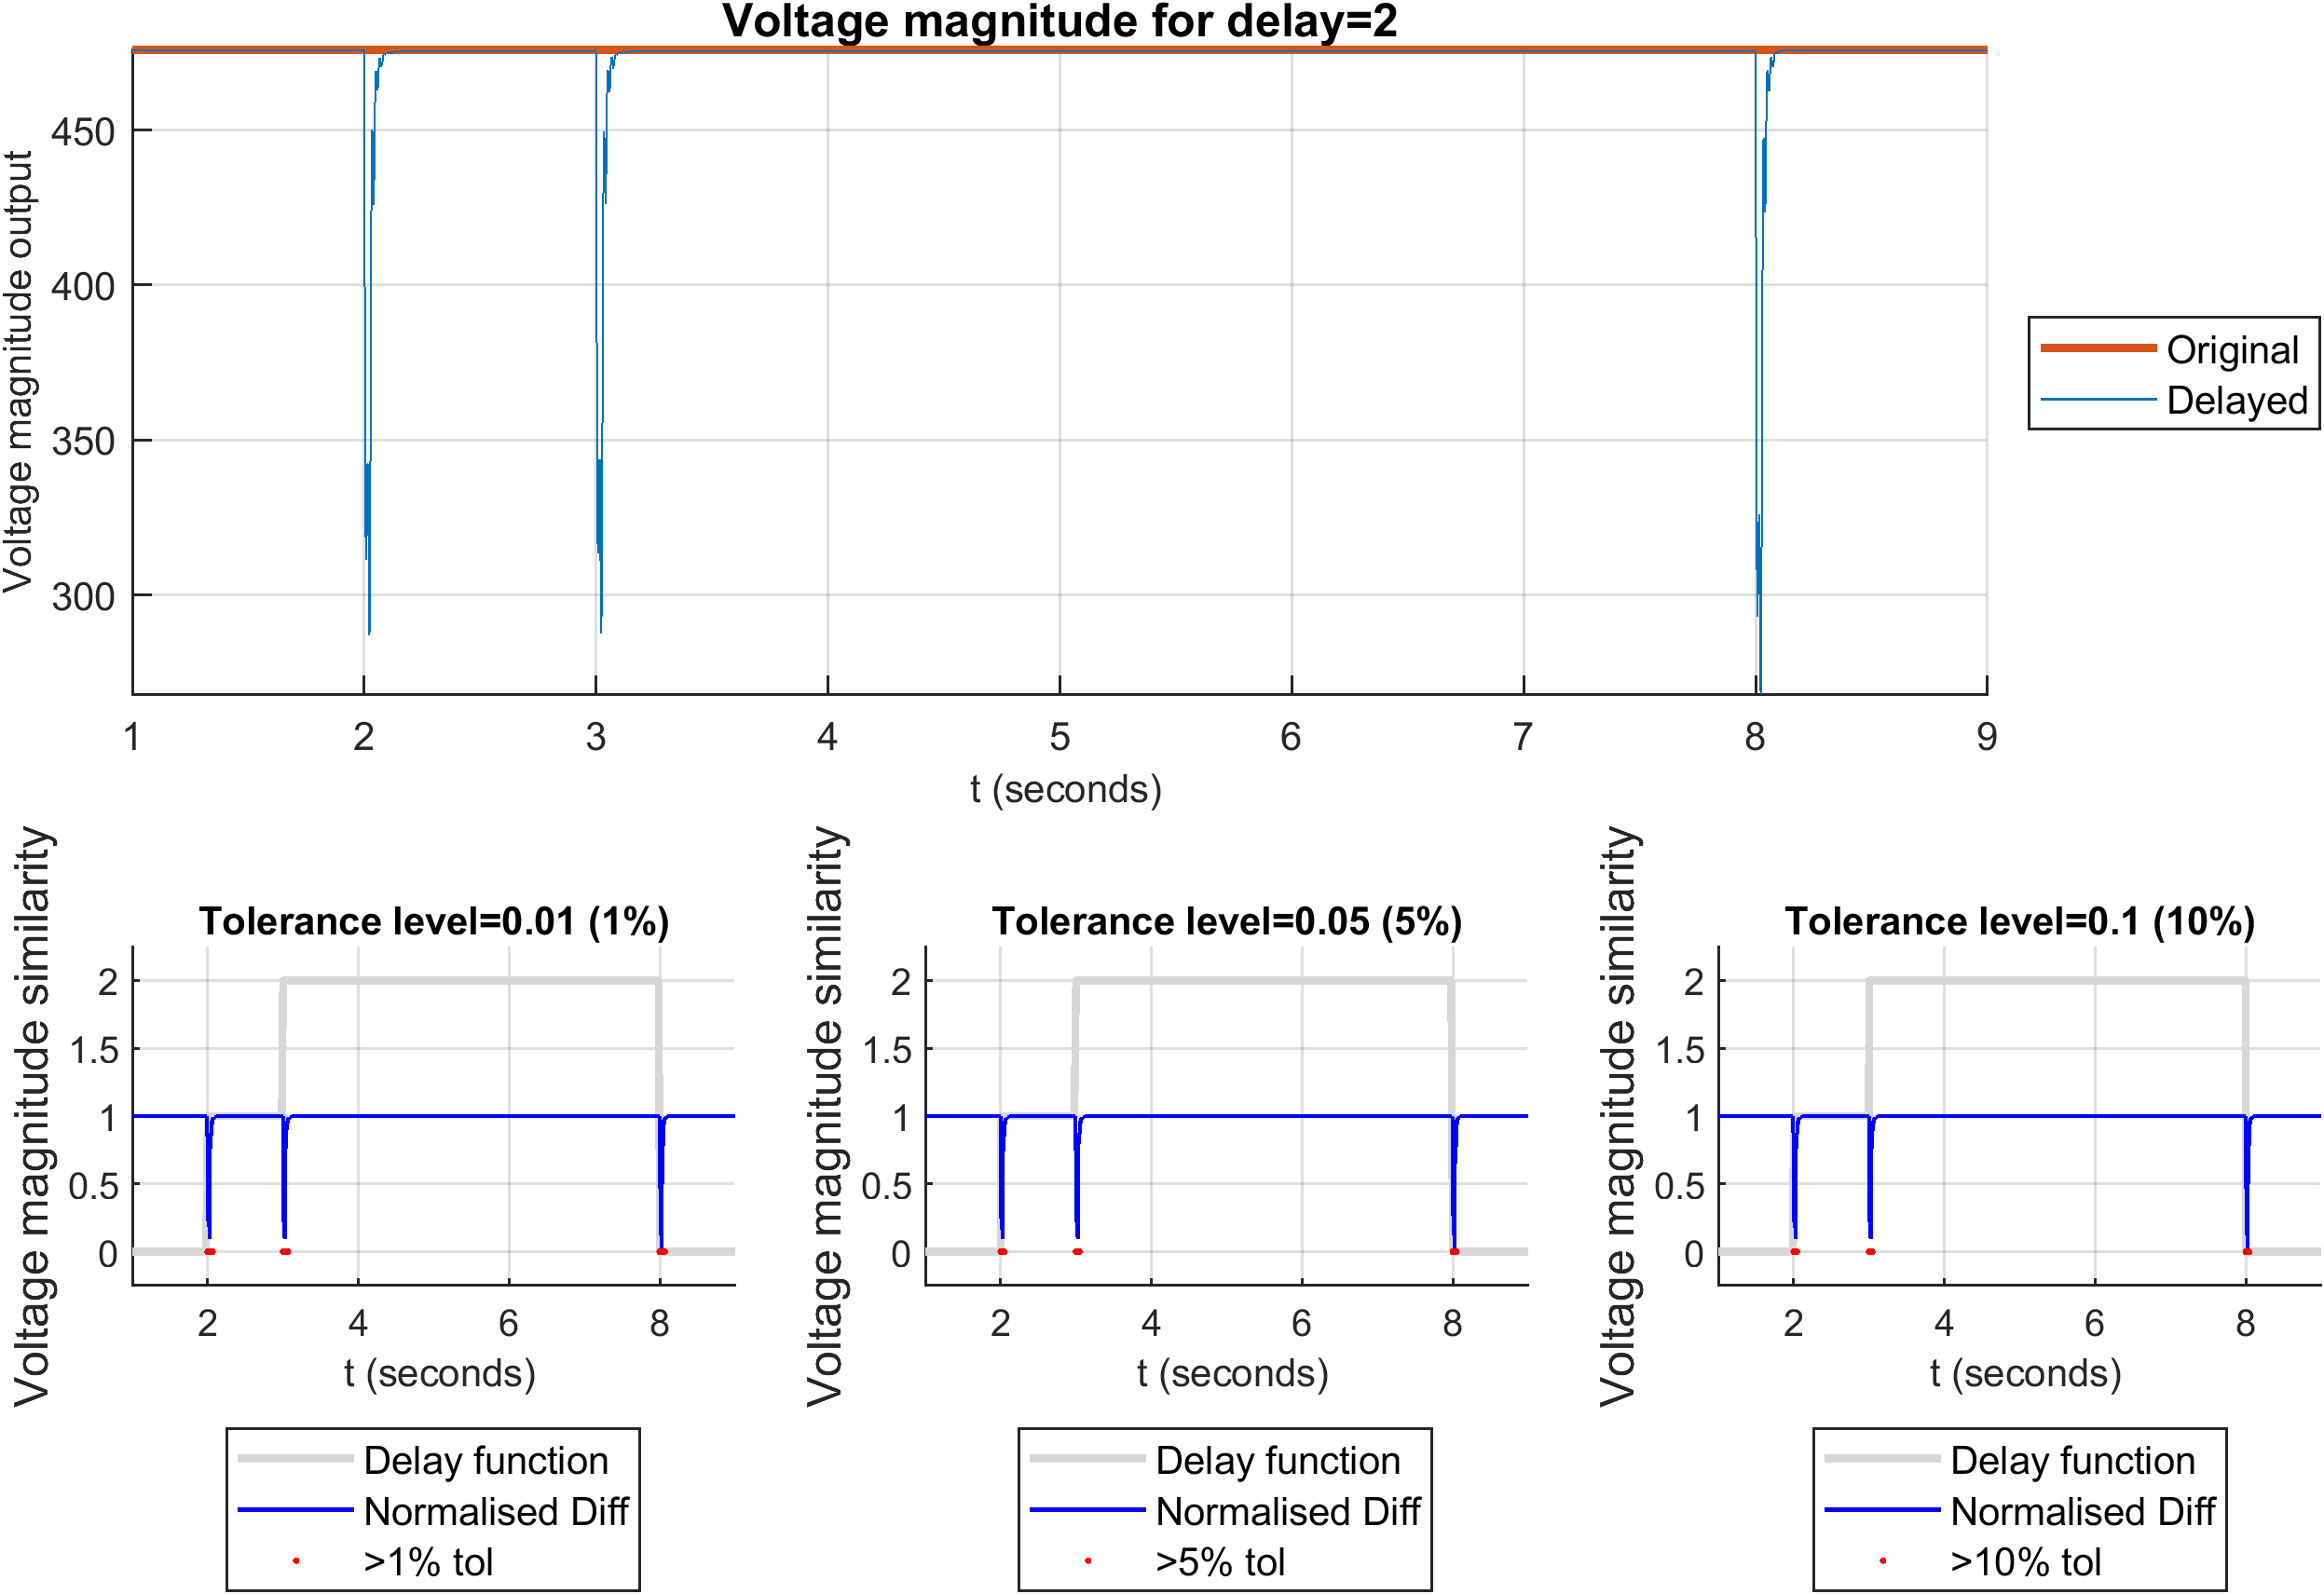
\includegraphics[width=0.95\textwidth]{PMUsim-figures/DelayOf_2/Step_vMagnitude.png}} \\ 
    \fbox{     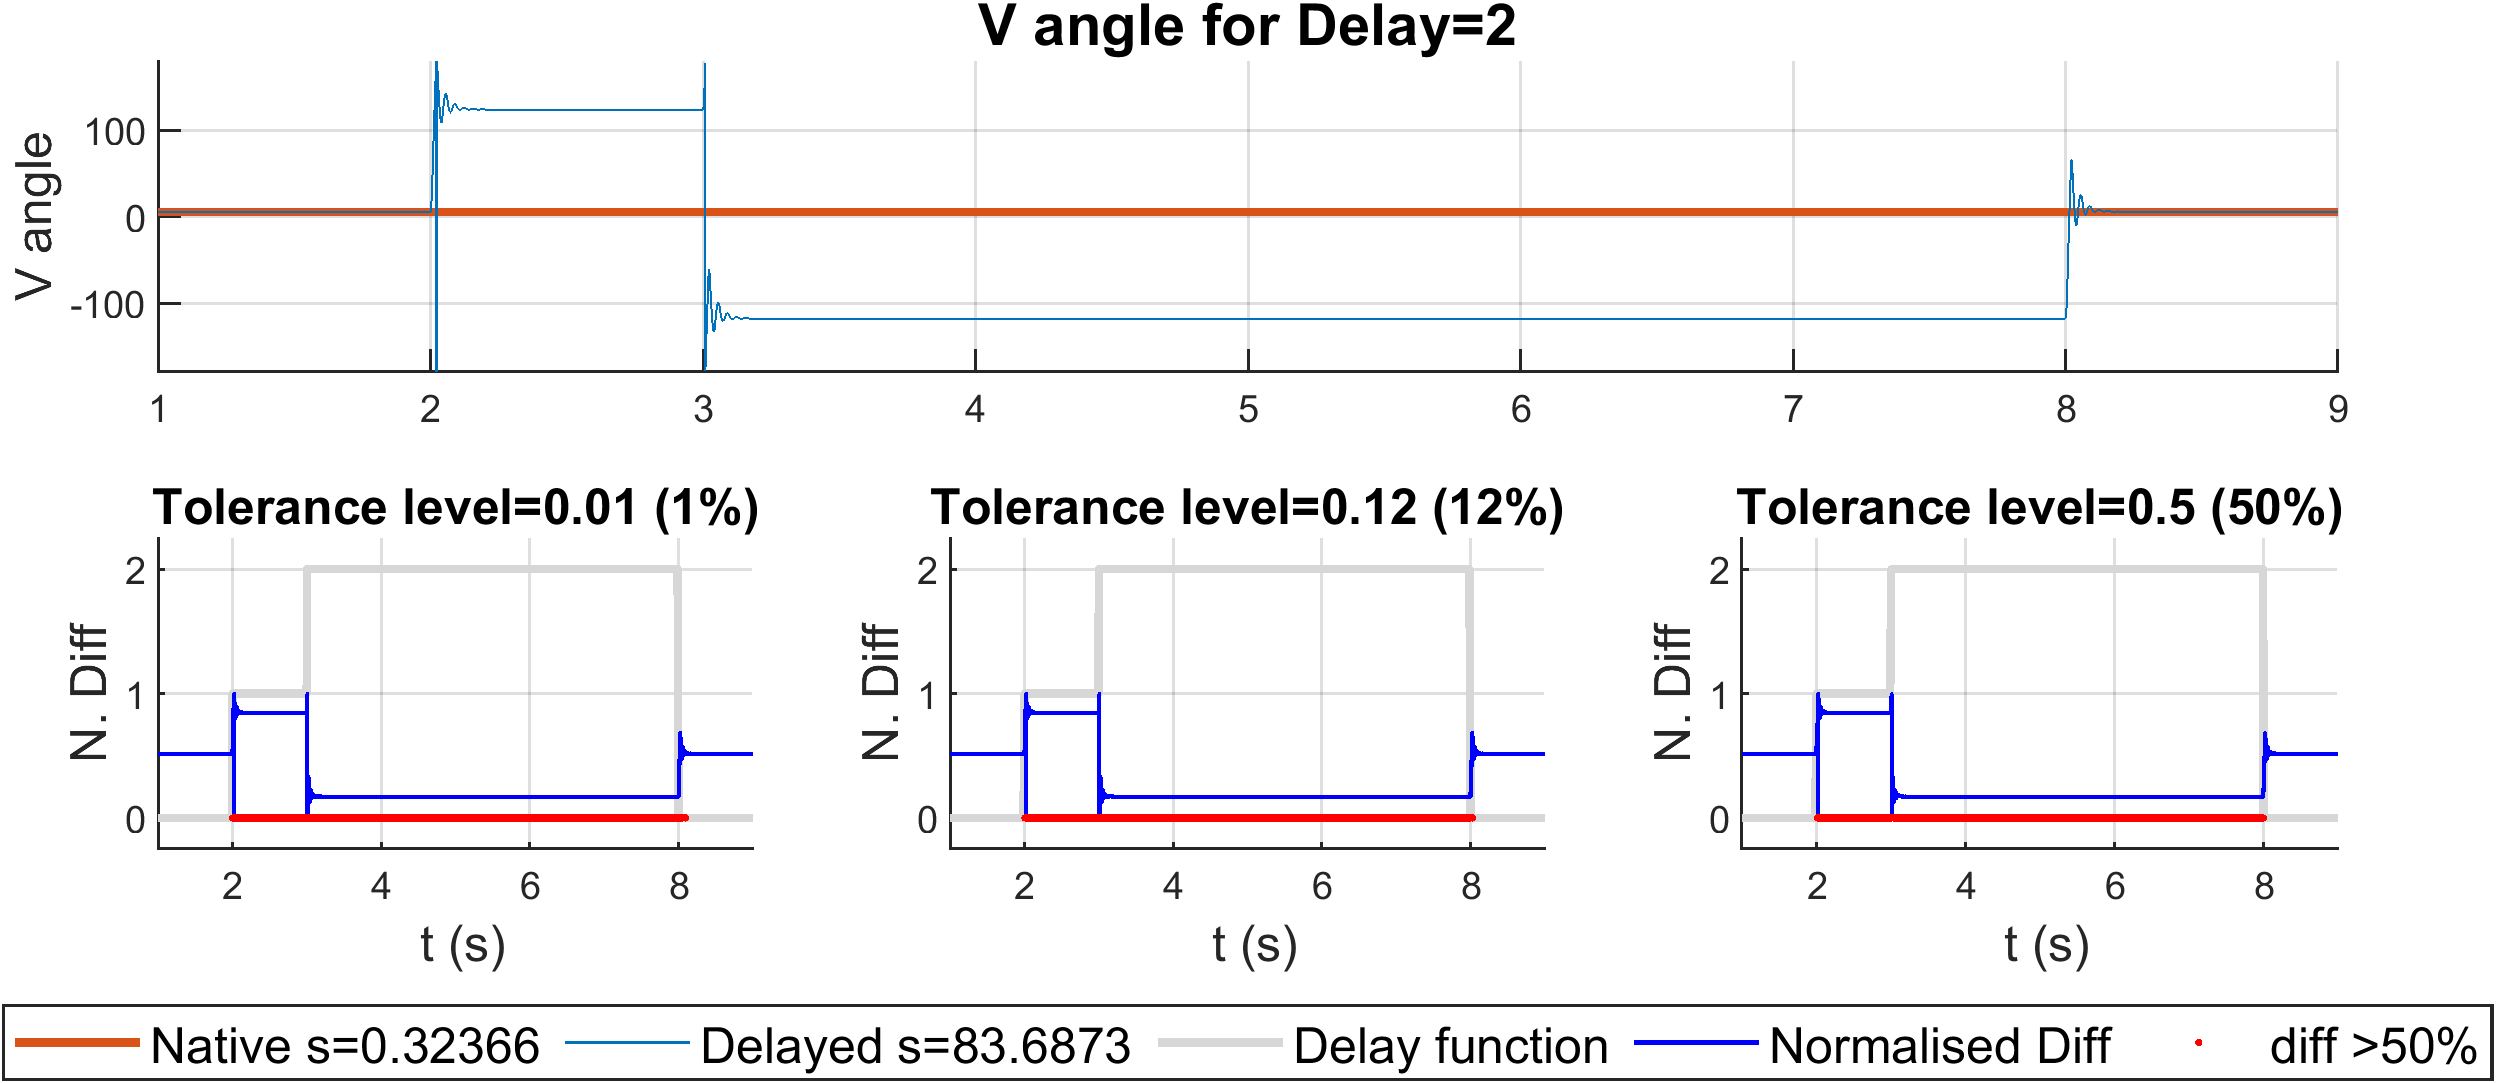
\includegraphics[width=0.95\textwidth]{PMUsim-figures/DelayOf_2/Step_vAngle.png}} \\ 
  
   \fbox{    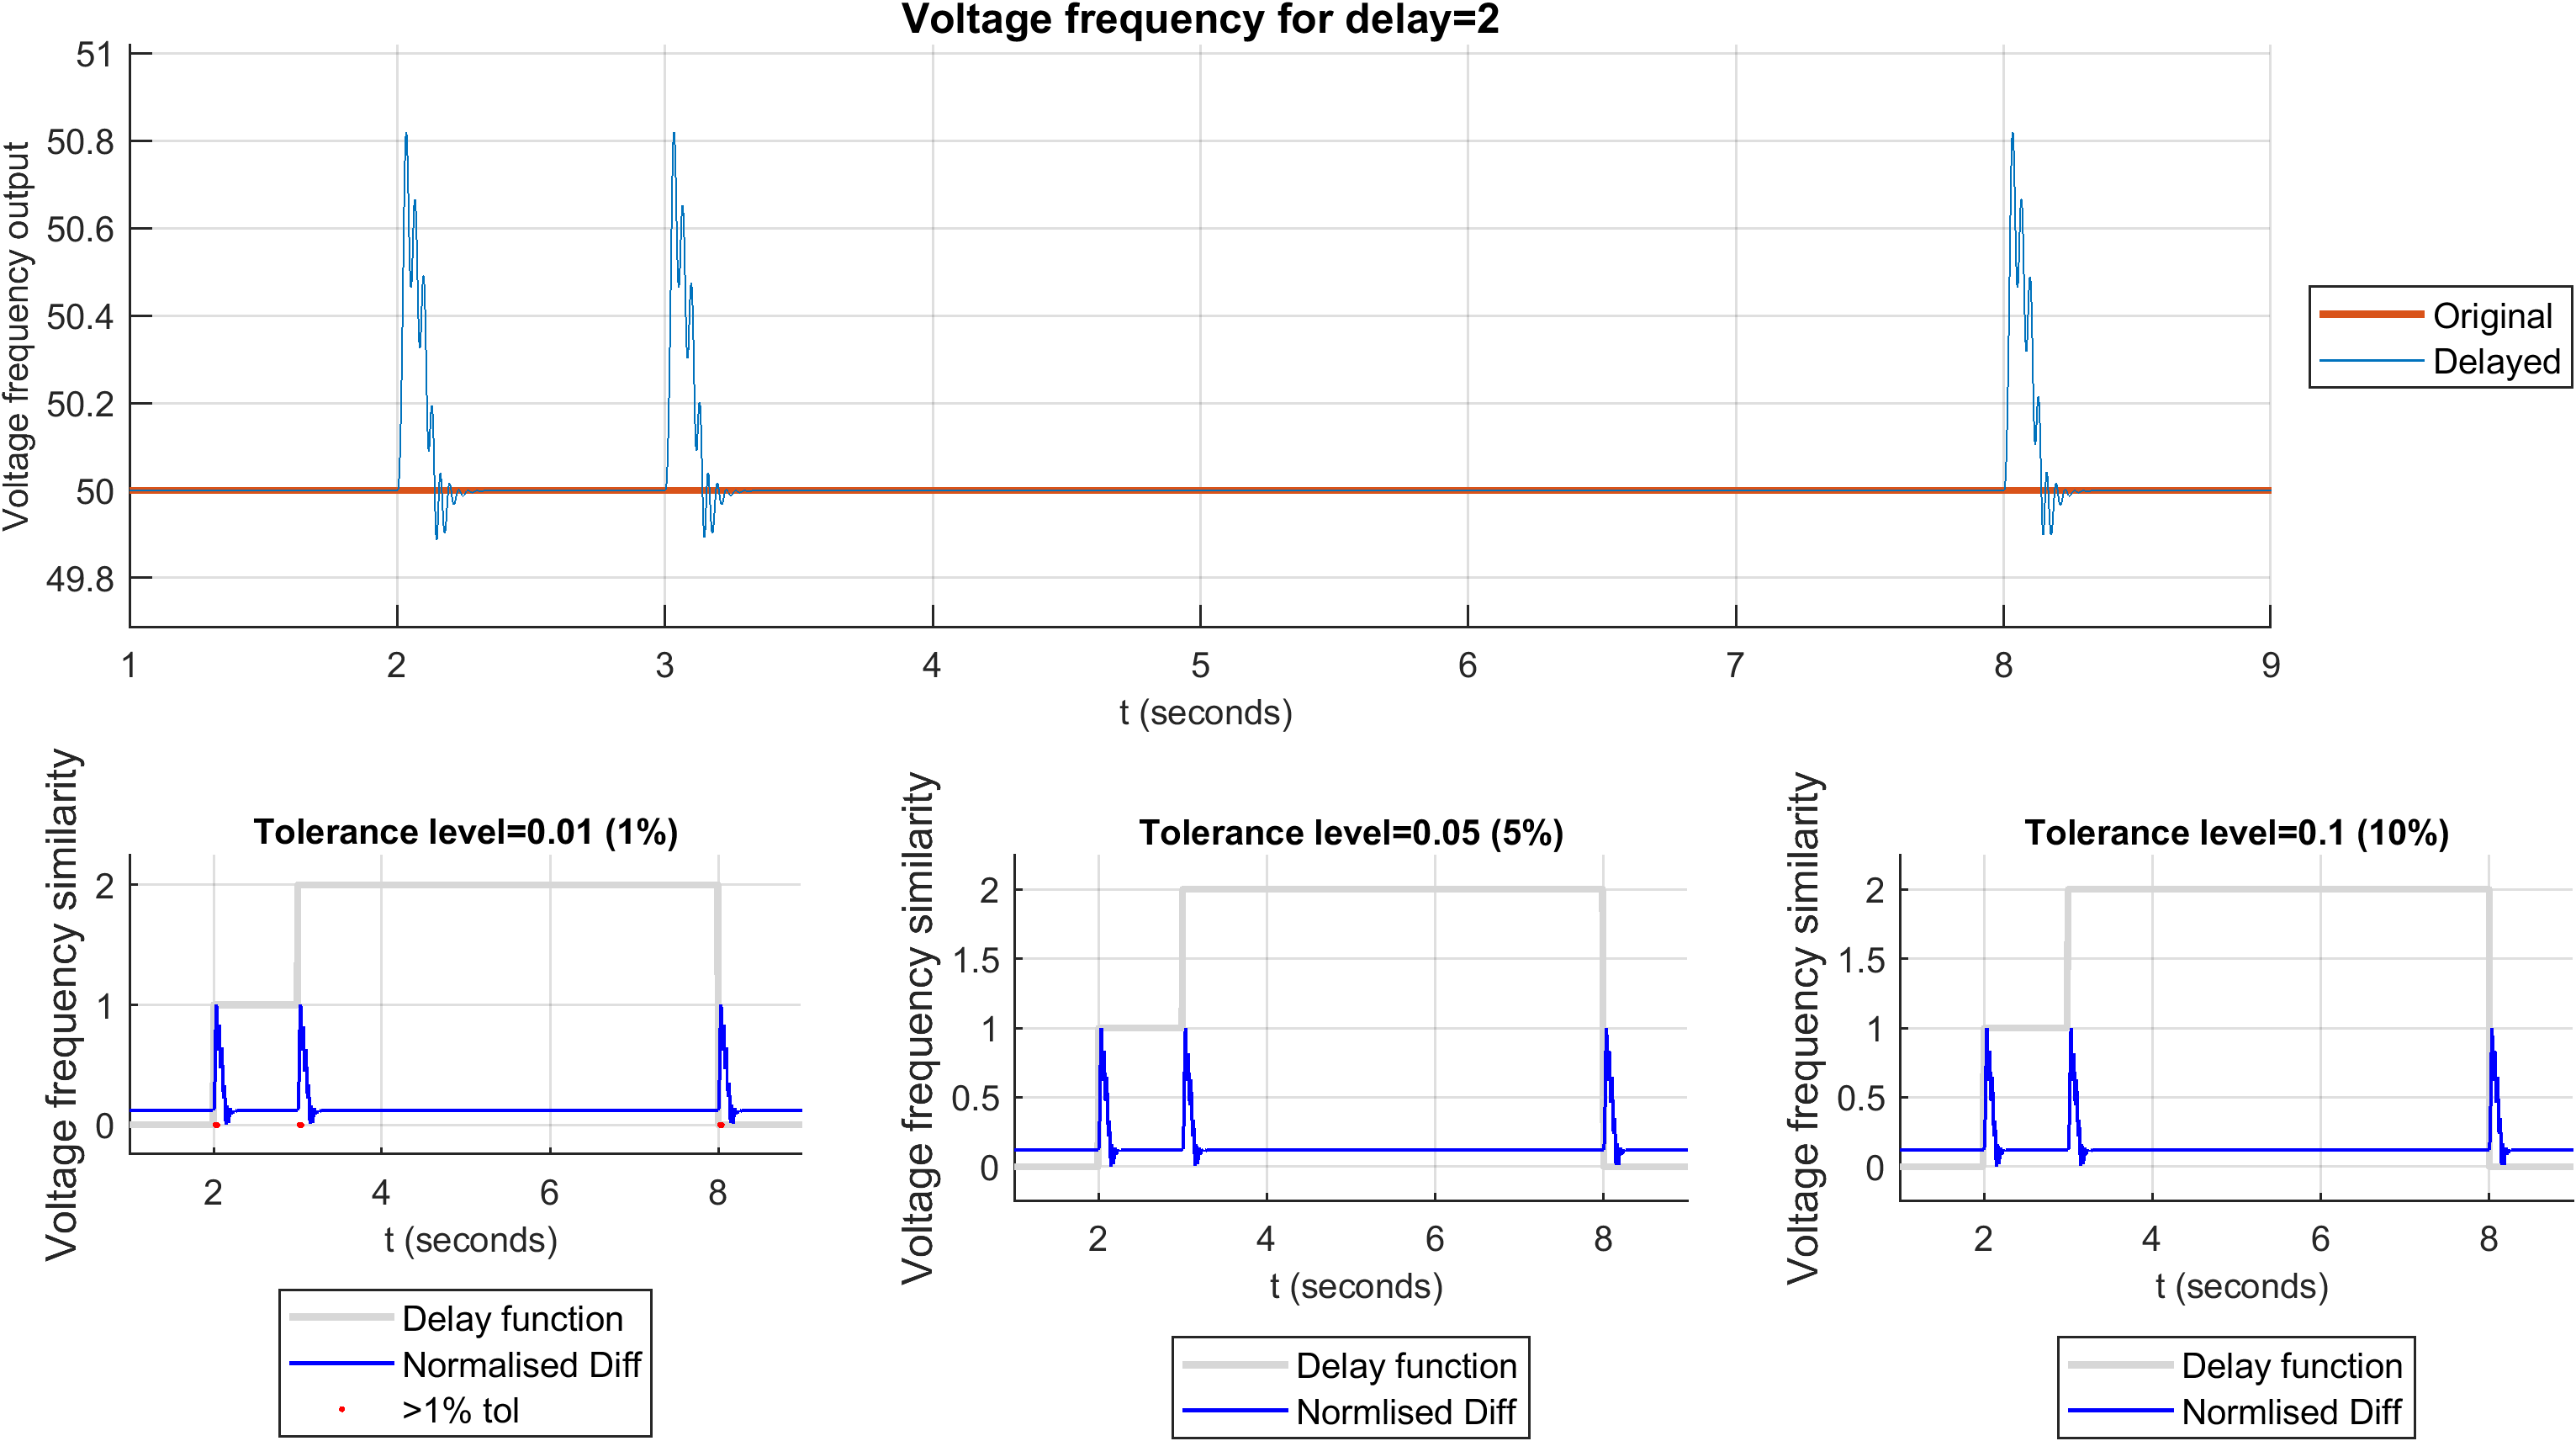
\includegraphics[width=0.95\textwidth]{PMUsim-figures/DelayOf_2/Step_vFrequency.png}}


  \end{tabular}
\label{fig:VoltageStepWiseDelayTwo}
\caption{Results for Voltage Output for Step-Wise Delay equal to Two }
\end{figure}
\newpage
\begin{figure}[H]
\begin{tabular}{c}
  \fbox{  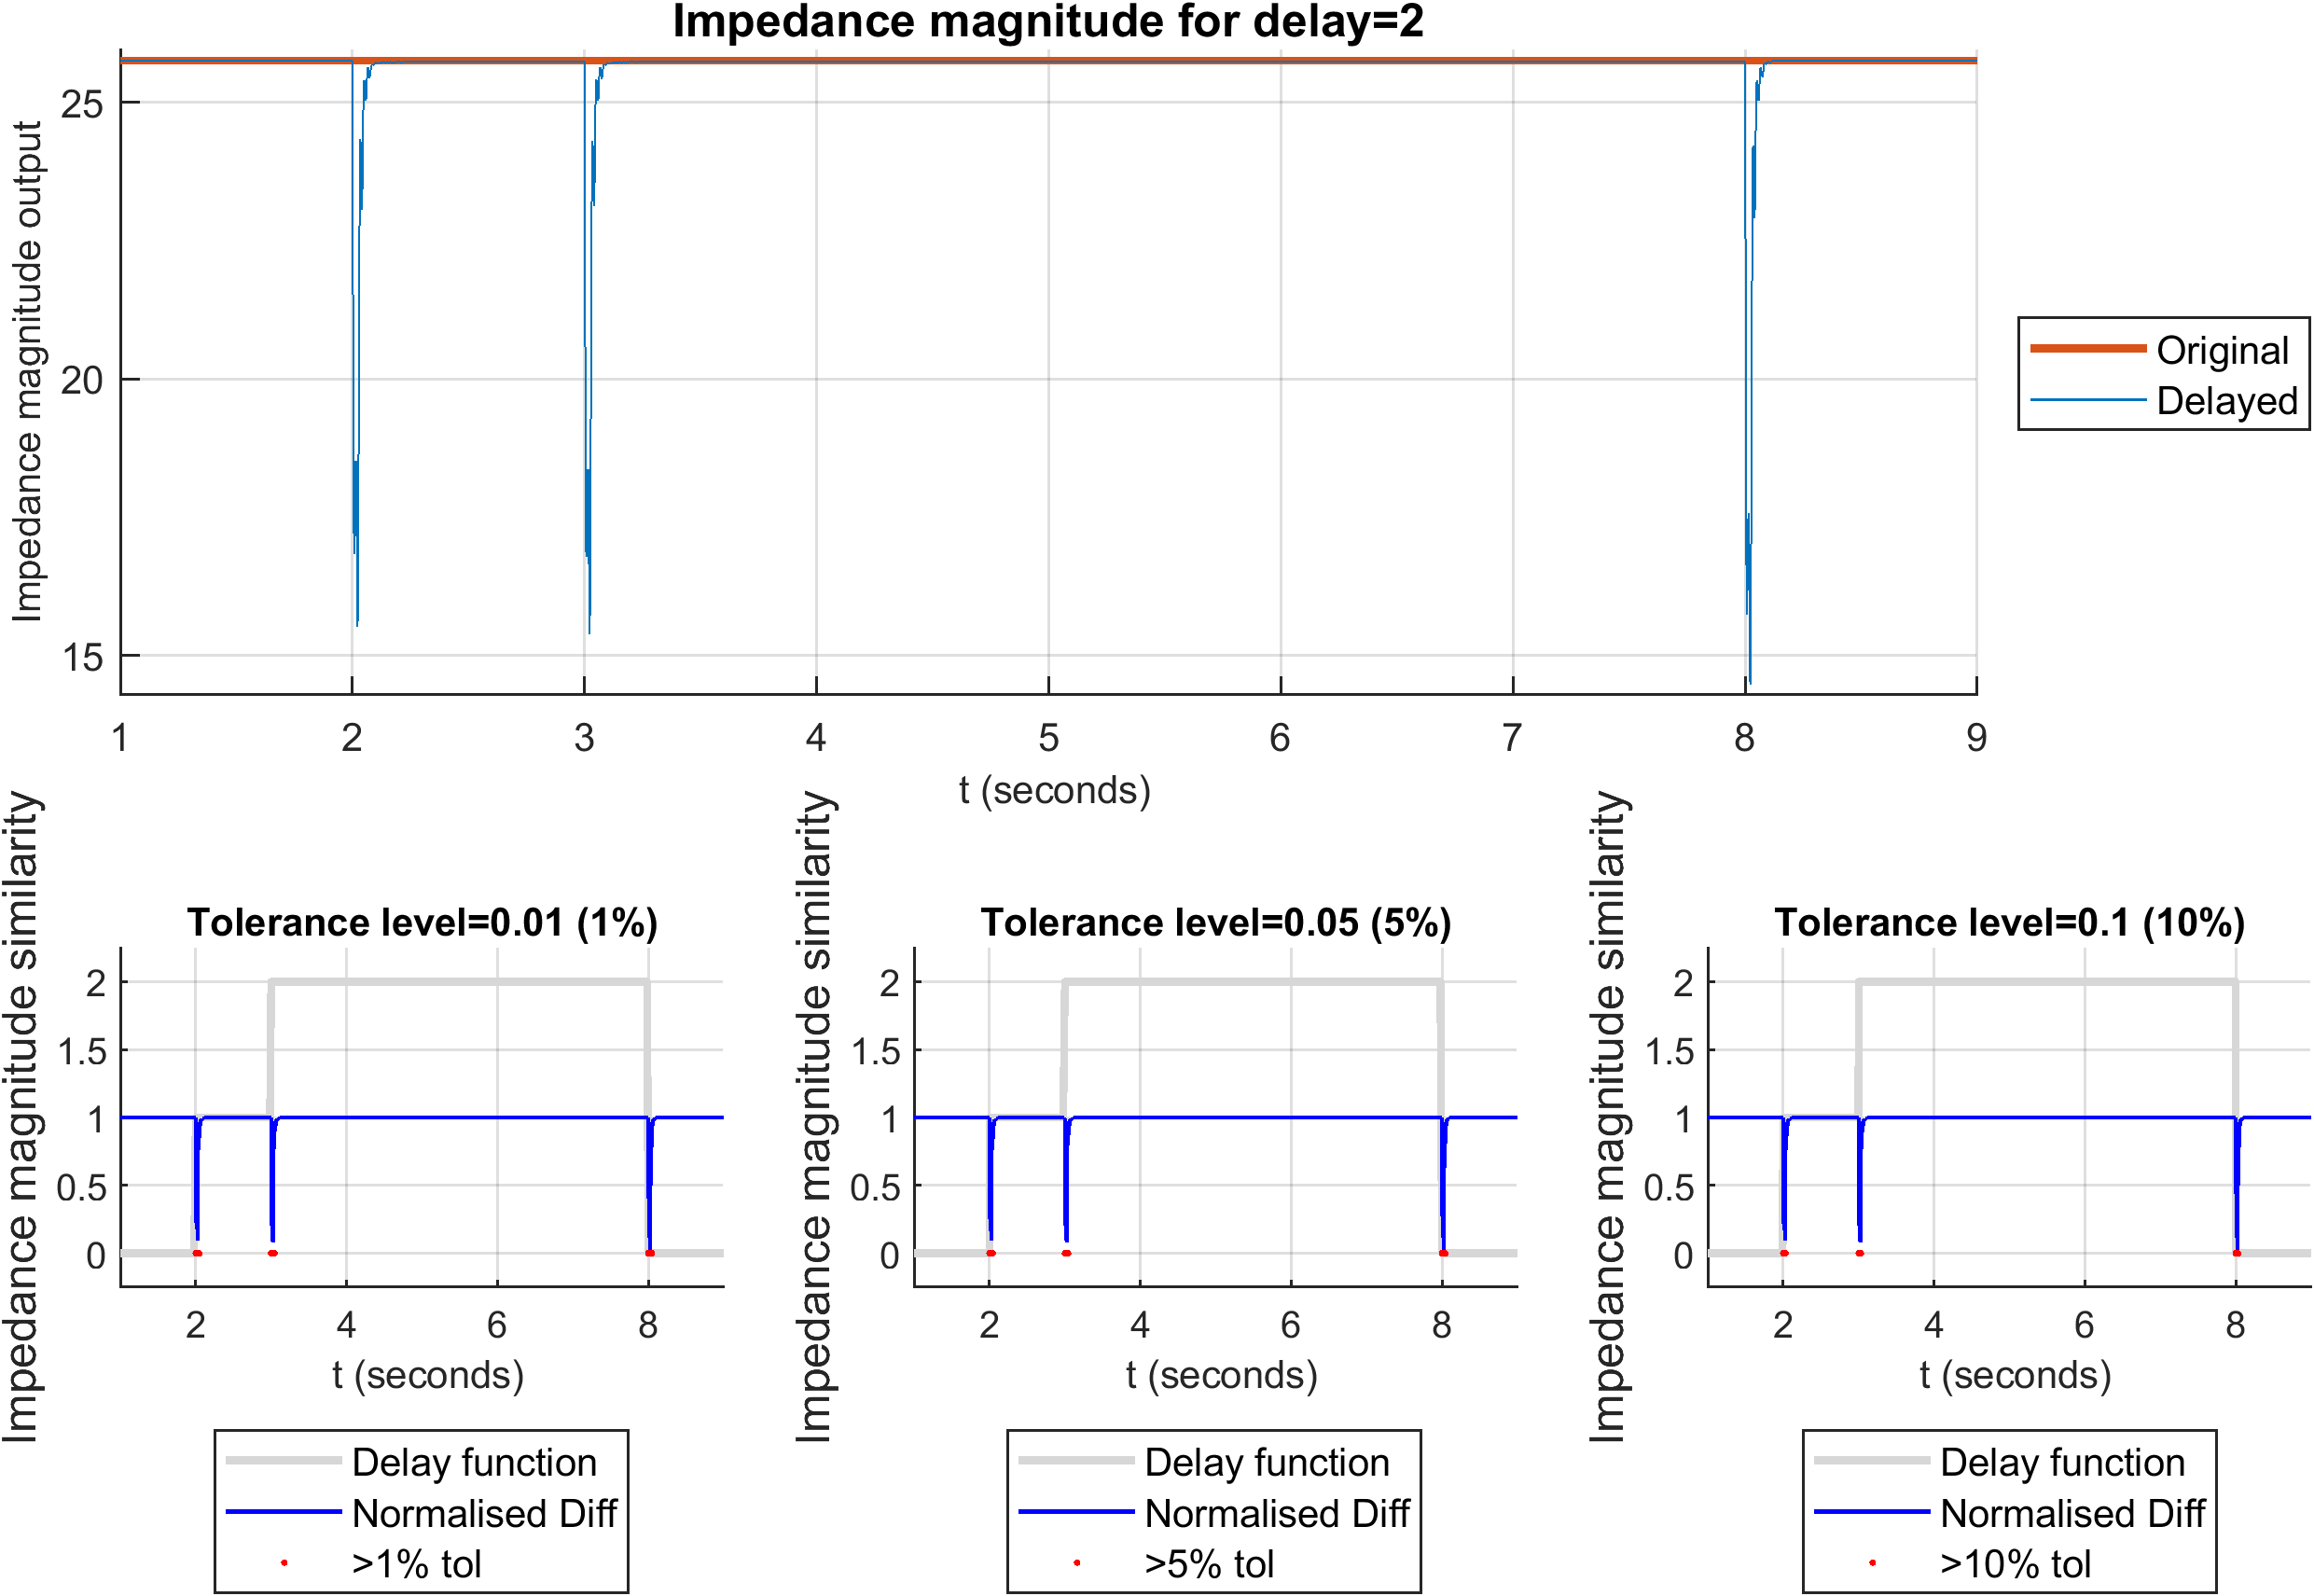
\includegraphics[width=0.95\textwidth]{PMUsim-figures/DelayOf_2/Step_iMagnitude.png}} \\ 
   \fbox{     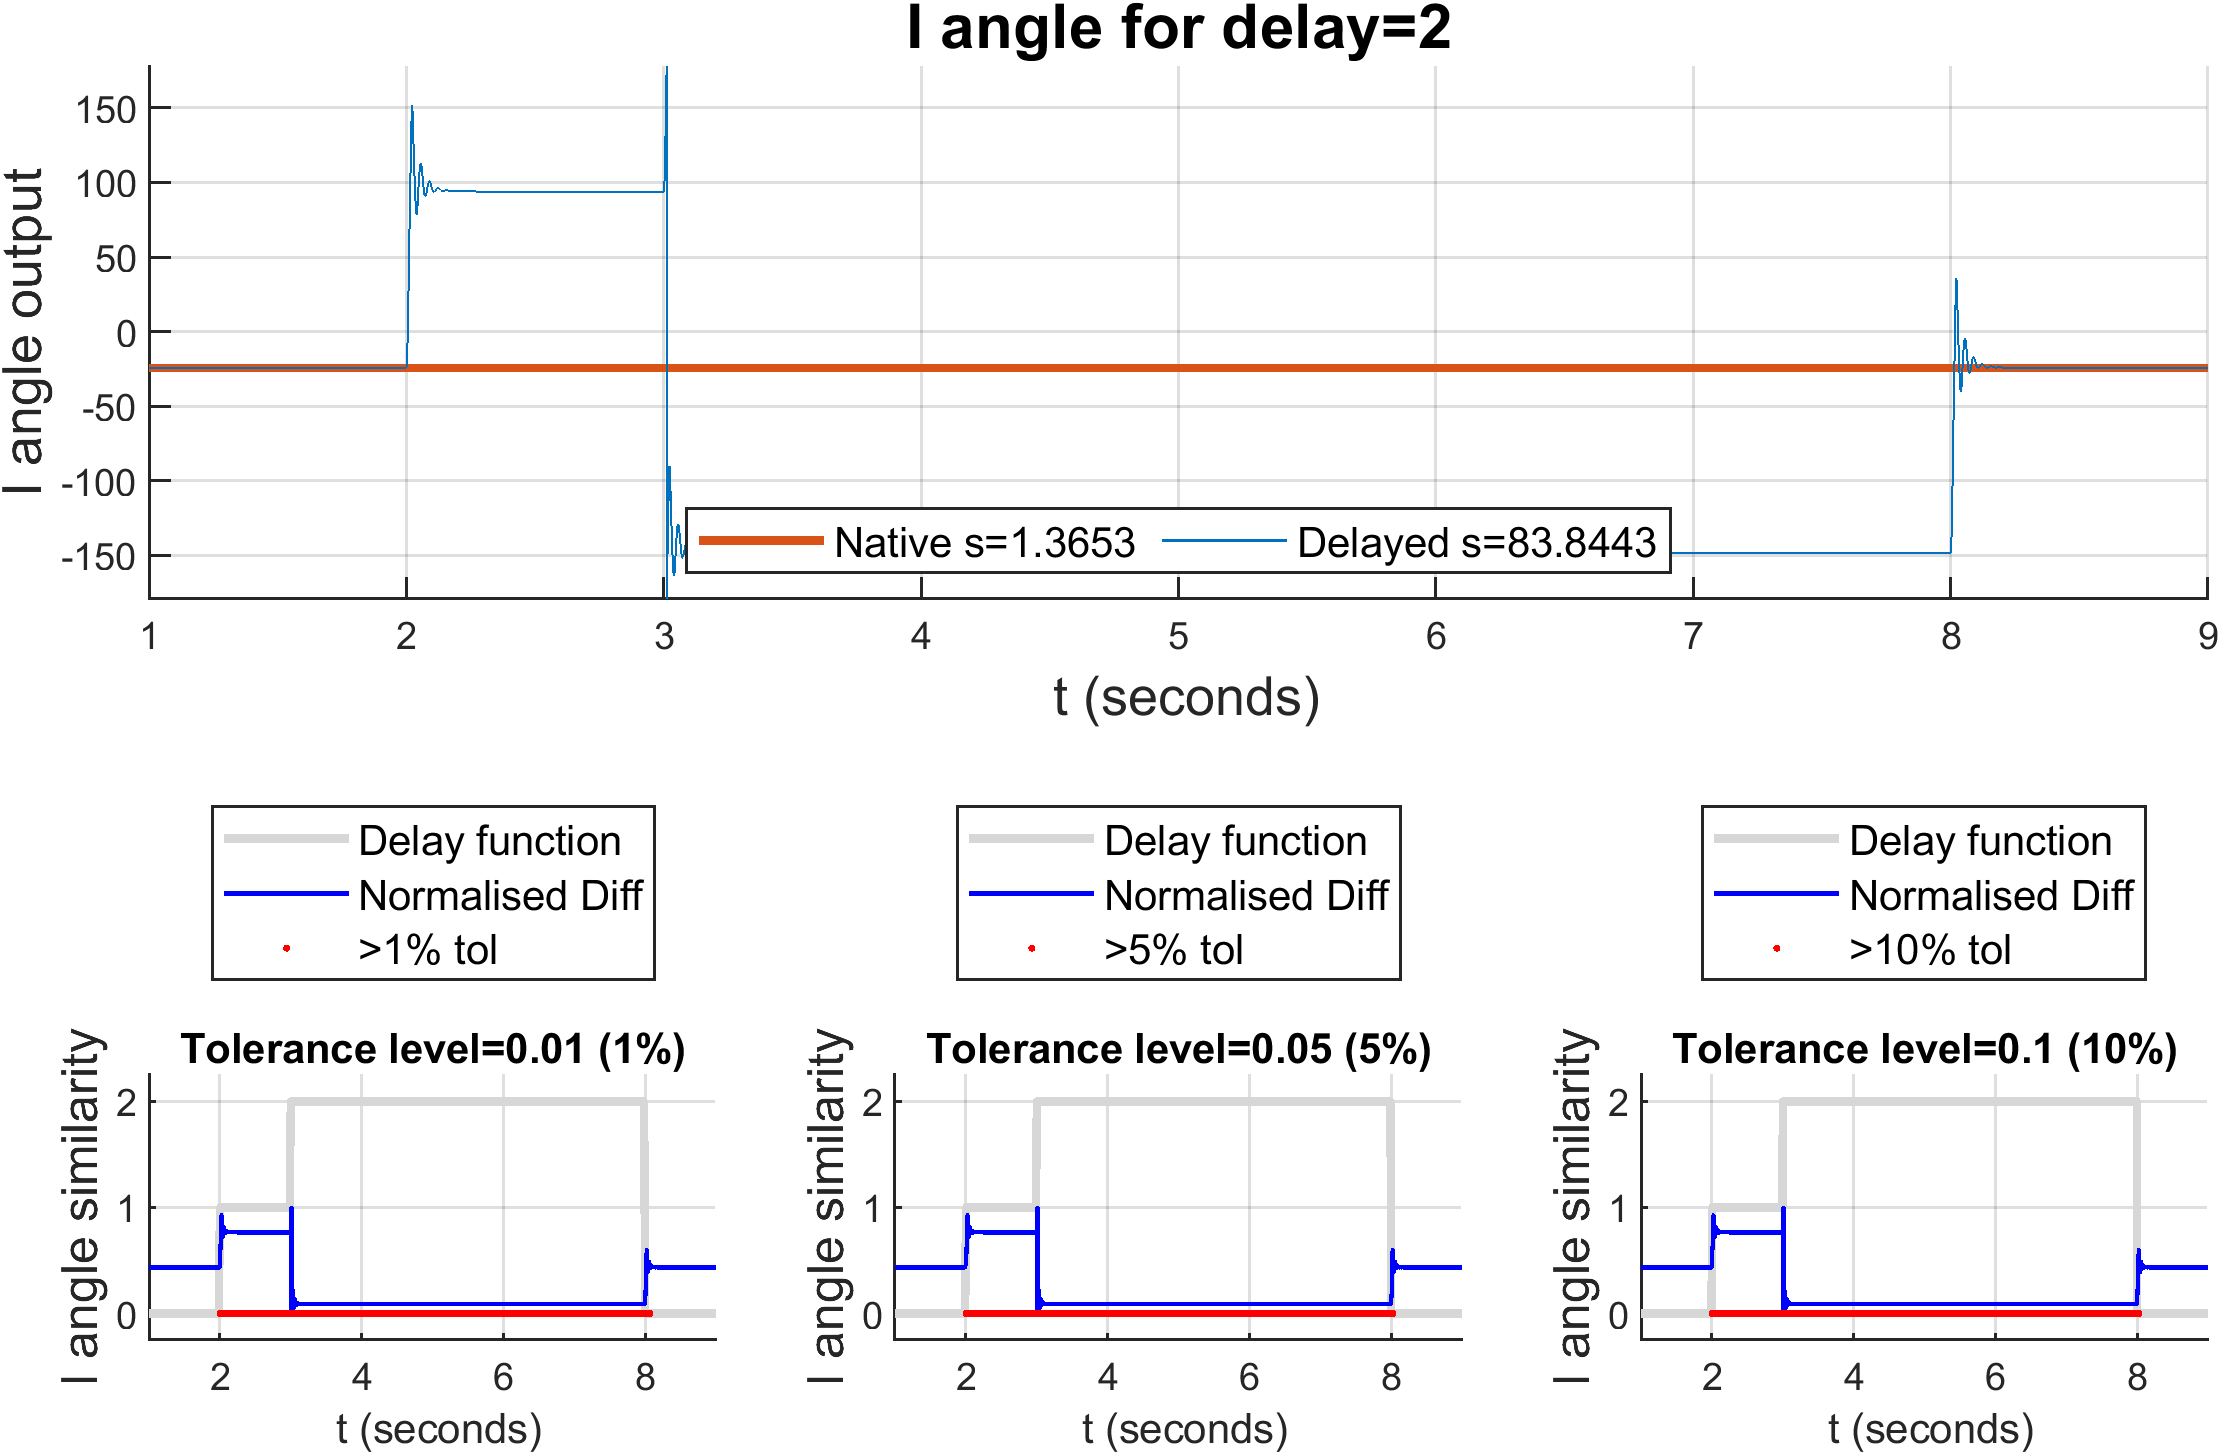
\includegraphics[width=0.95\textwidth]{PMUsim-figures/DelayOf_2/Step_iAngle.png}} \\   
   \fbox{    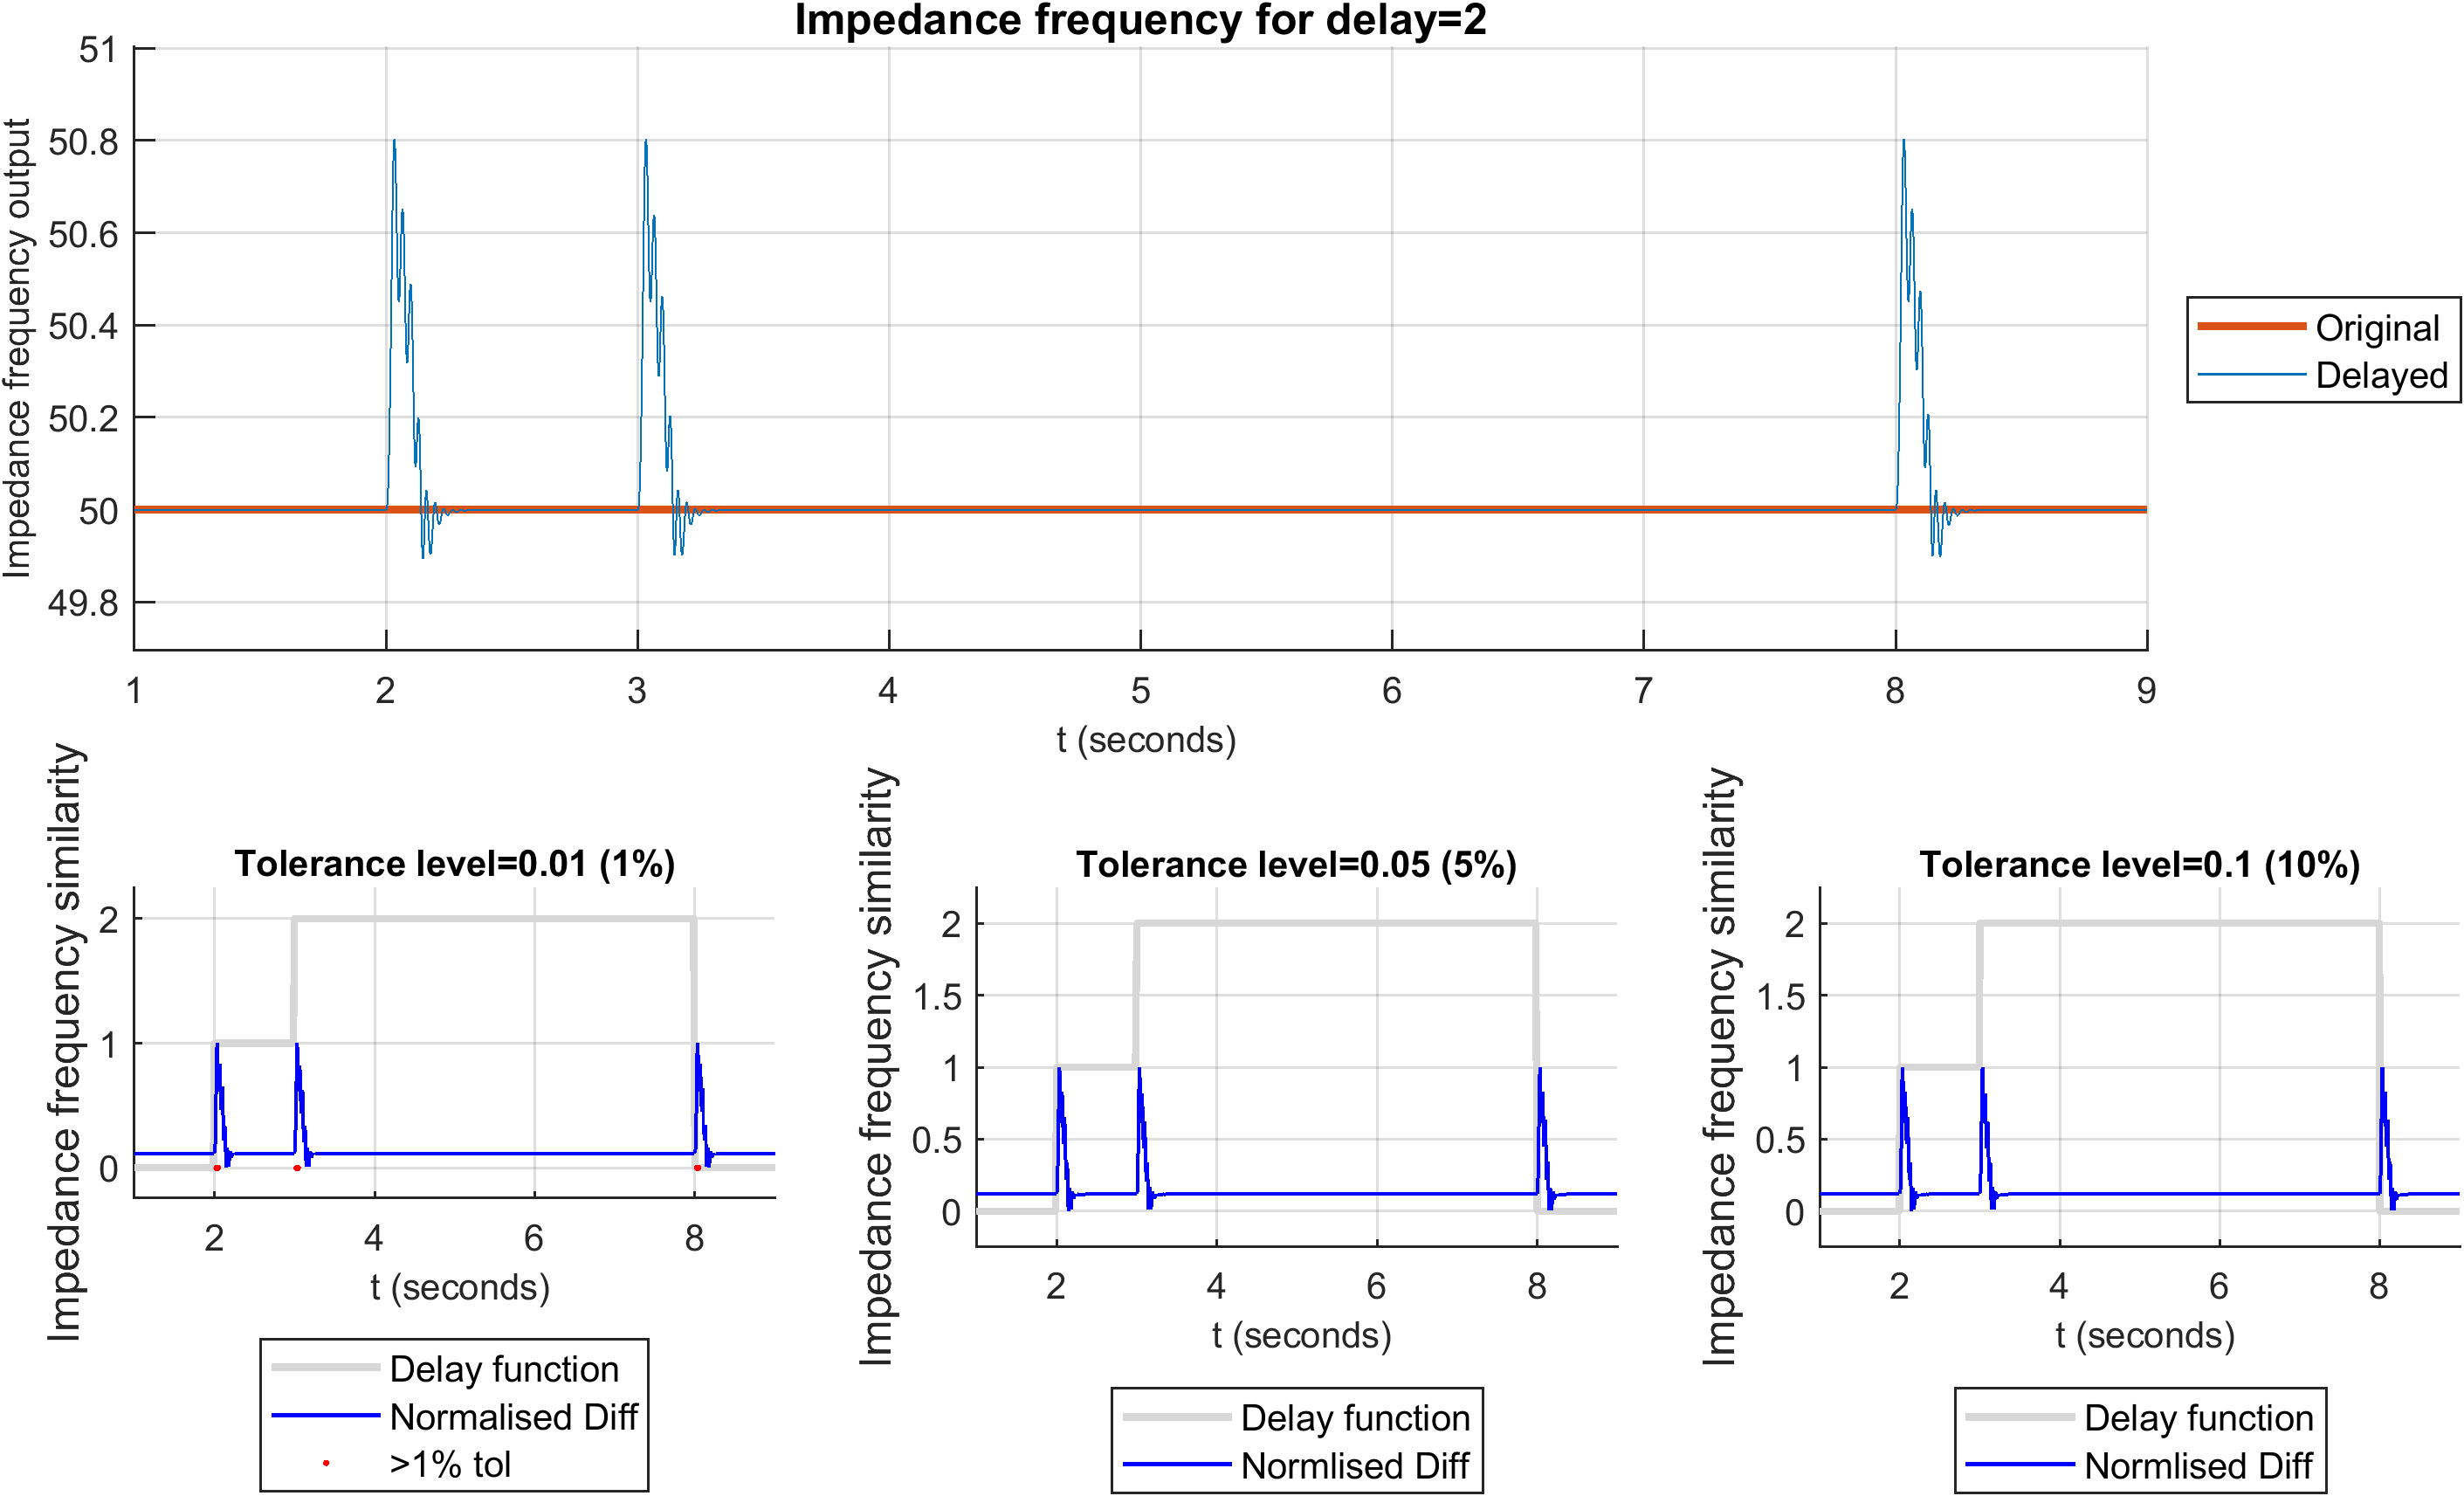
\includegraphics[width=0.95\textwidth]{PMUsim-figures/DelayOf_2/Step_iFrequency.png}} 


  \end{tabular}
\label{fig:ImpedanceStepWiseDelayDelayTwo}
\caption{Results for Impedance Output for Step-Wise Delay equal to Two }
\end{figure}





\newpage
\begin{figure}[H]
\begin{tabular}{c}
  \fbox{  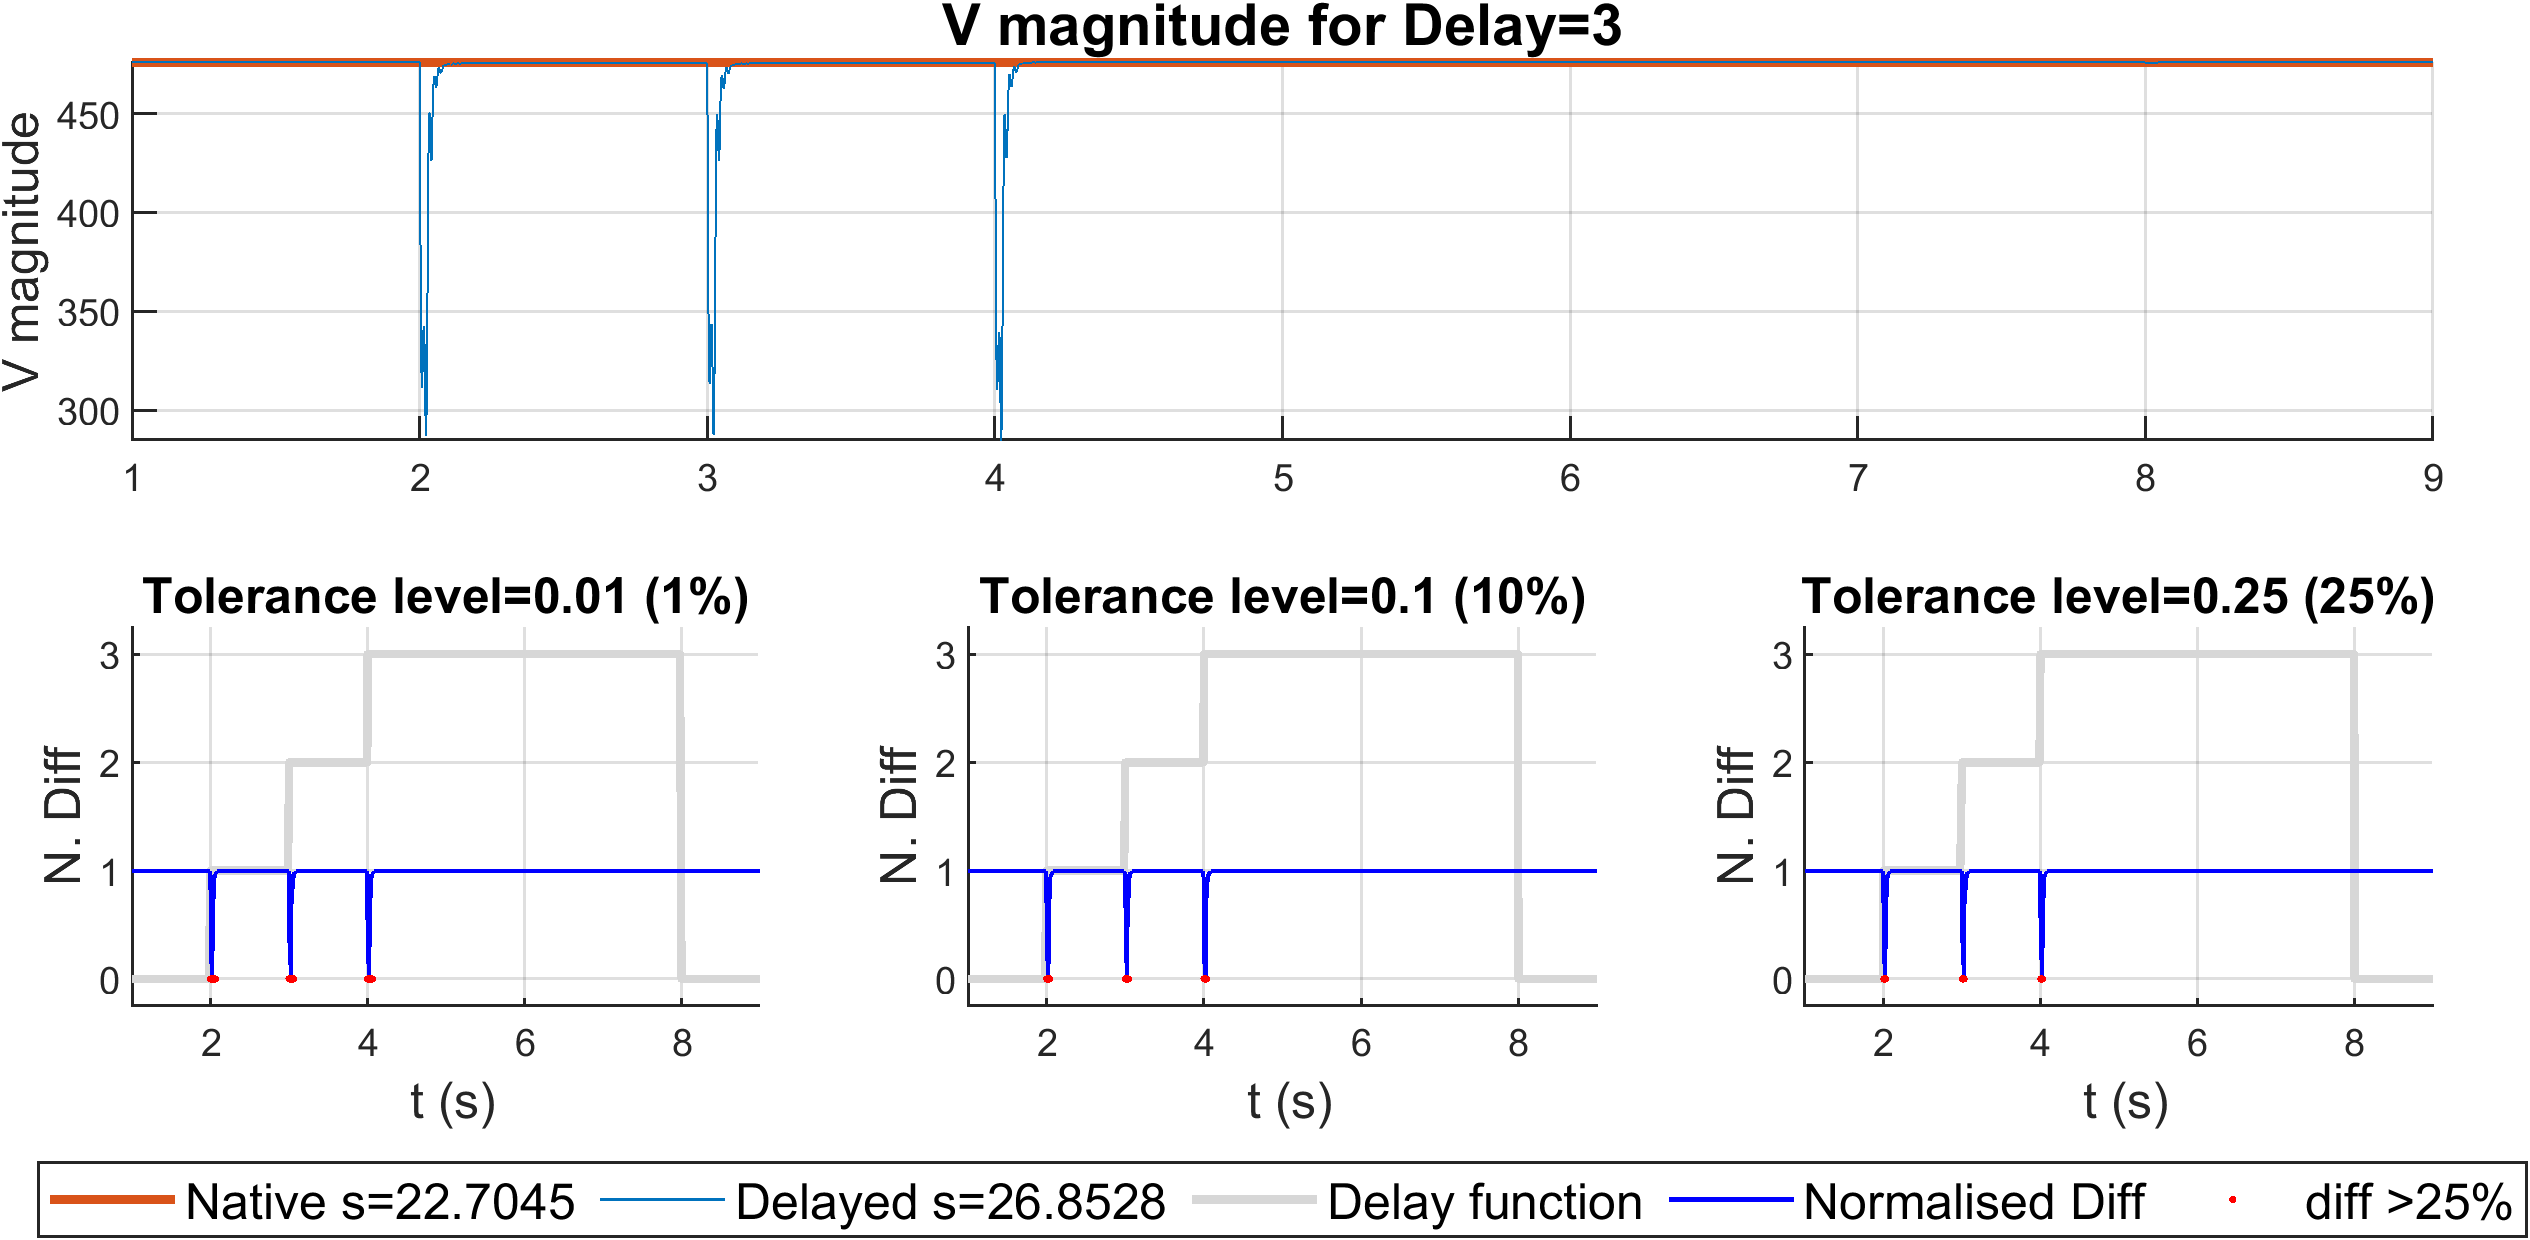
\includegraphics[width=0.95\textwidth]{PMUsim-figures/DelayOf_3/Step_vMagnitude.png}} \\ 
   \fbox{     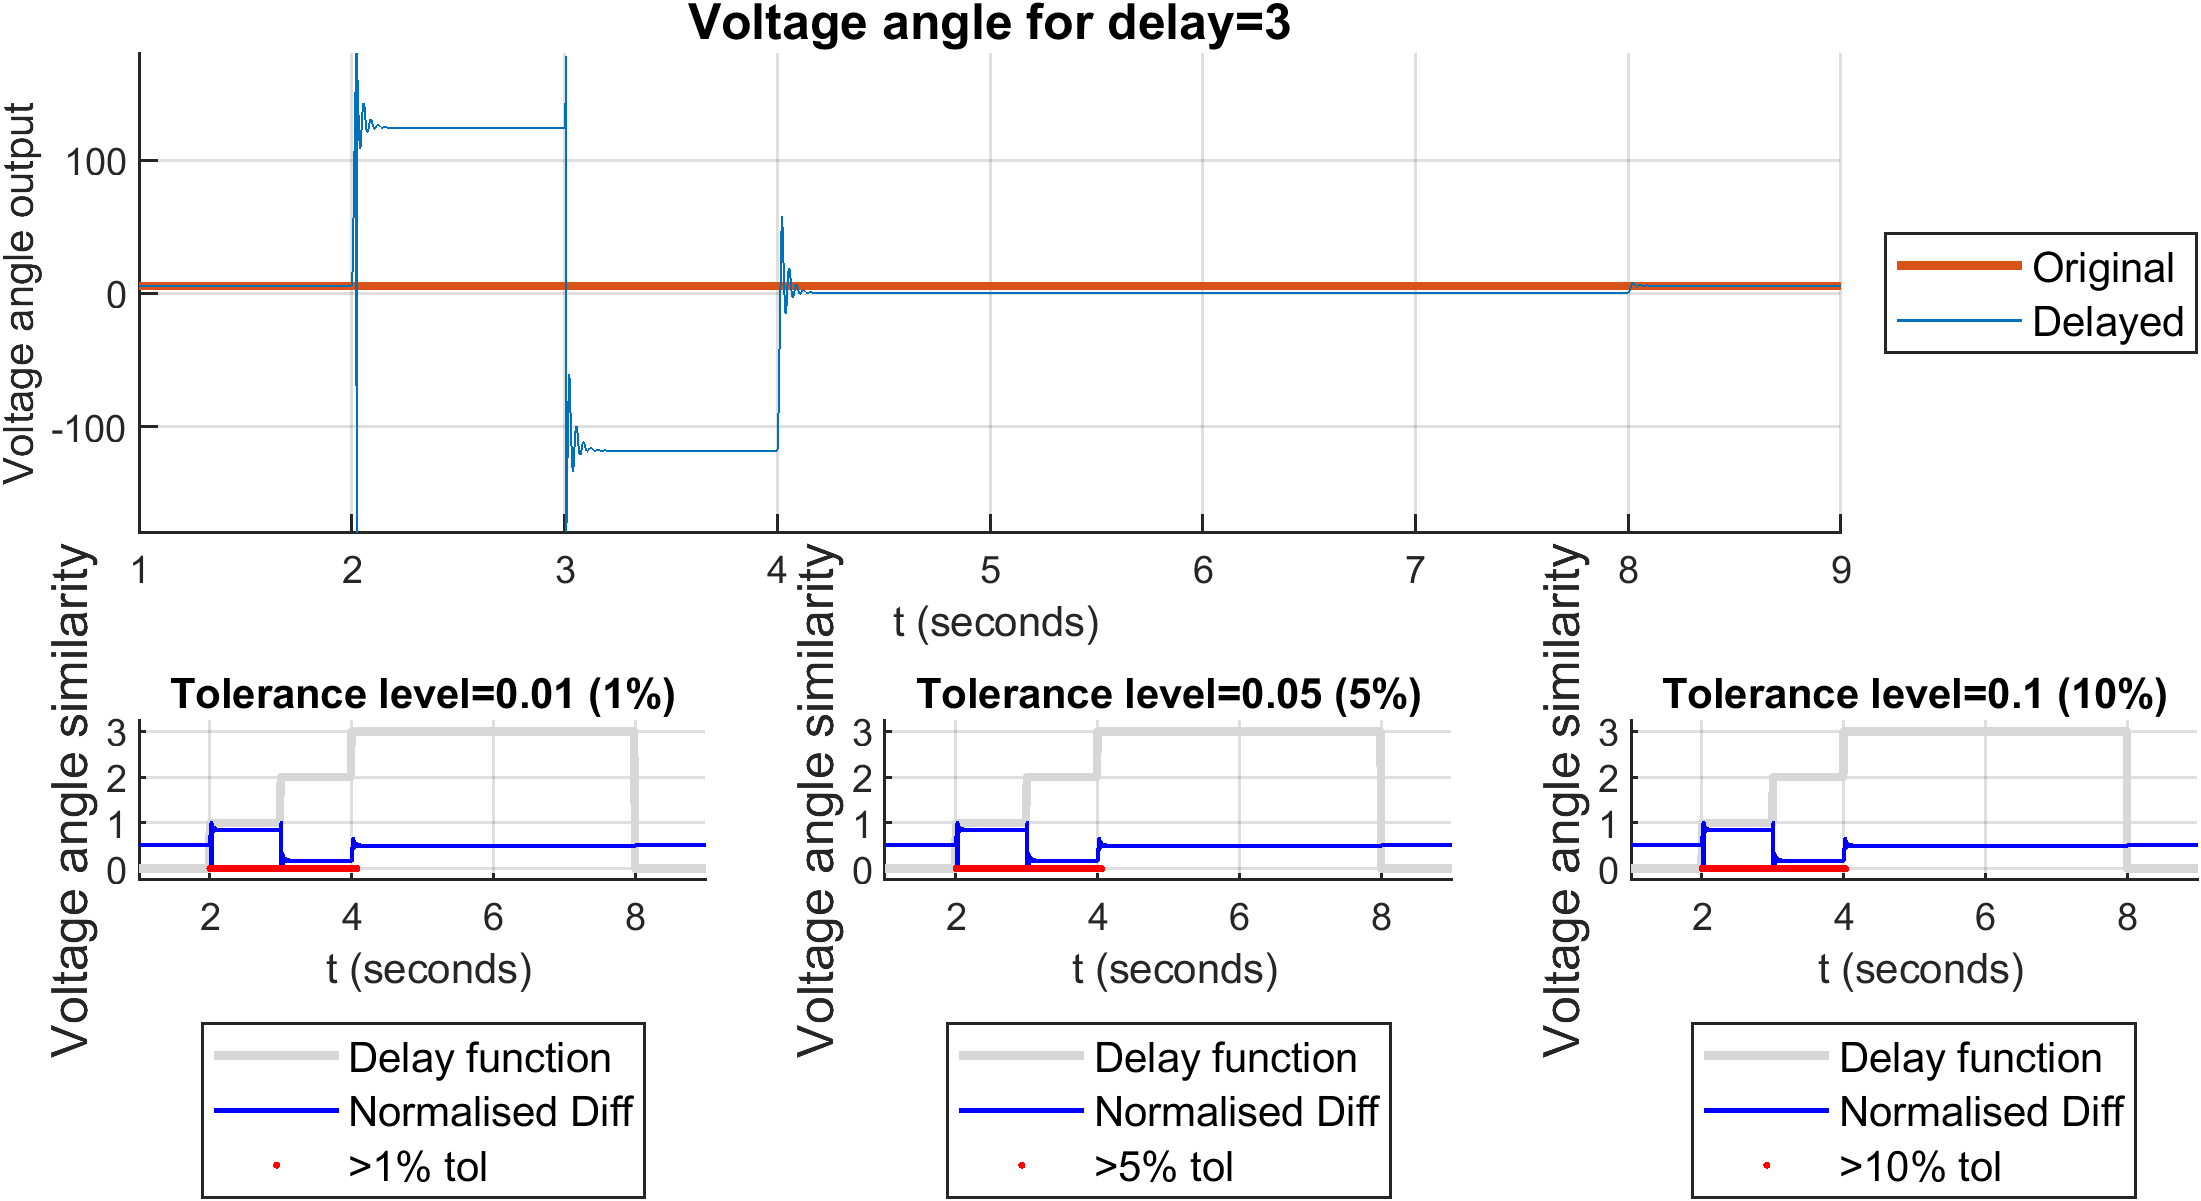
\includegraphics[width=0.95\textwidth]{PMUsim-figures/DelayOf_3/Step_vAngle.png}} \\    
   \fbox{    \includegraphics[width=0.95\textwidth]{PMUsim-figures/DelayOf_3/Step_vFrequency.png}}

  \end{tabular}
\label{fig:VoltageStepWiseDelayThree}
\caption{Results for Voltage Output for Step-Wise Delay equal to Three }
\end{figure}
\newpage
\begin{figure}[H]
\begin{tabular}{c}
  \fbox{  \includegraphics[width=0.95\textwidth]{PMUsim-figures/DelayOf_3/Step_iMagnitude.png}} \\ 
   \fbox{     \includegraphics[width=0.95\textwidth]{PMUsim-figures/DelayOf_3/Step_iAngle.png}} \\  
   \fbox{    \includegraphics[width=0.95\textwidth]{PMUsim-figures/DelayOf_3/Step_iFrequency.png}}

    

  \end{tabular}
\label{fig:ImpedanceStepWiseDelayThree}
\caption{Results for Impedance Output for Step-Wise Delay equal to Three }
\end{figure}






\newpage
\begin{figure}[H]
\begin{tabular}{c}
  \fbox{  \includegraphics[width=0.95\textwidth]{PMUsim-figures/DelayOf_4/Step_vMagnitude.png}} \\ 
   \fbox{     \includegraphics[width=0.95\textwidth]{PMUsim-figures/DelayOf_4/Step_vAngle.png}} \\    
   \fbox{    \includegraphics[width=0.95\textwidth]{PMUsim-figures/DelayOf_4/Step_vFrequency.png}}


  \end{tabular}
\label{fig:VoltageStepWiseDelayFour}
\caption{Results for Voltage Output for Step-Wise Delay equal to Four }
\end{figure}
\newpage
\begin{figure}[H]
\begin{tabular}{c}
  \fbox{  \includegraphics[width=0.95\textwidth]{PMUsim-figures/DelayOf_4/Step_iMagnitude.png}} \\ 
    \fbox{     \includegraphics[width=0.95\textwidth]{PMUsim-figures/DelayOf_4/Step_iAngle.png}}  \\  
   \fbox{    \includegraphics[width=0.95\textwidth]{PMUsim-figures/DelayOf_4/Step_iFrequency.png}} 


  \end{tabular}
\label{fig:ImpedanceStepWiseDelayFour}
\caption{Results for Impedance Output for Step-Wise Delay equal to Four }
\end{figure}




\newpage
\begin{figure}[H]
\begin{tabular}{c}
  \fbox{  \includegraphics[width=0.95\textwidth]{PMUsim-figures/DelayOf_5/Step_vMagnitude.png}} \\ 
  \fbox{     \includegraphics[width=0.95\textwidth]{PMUsim-figures/DelayOf_5/Step_vAngle.png}} \\    
   \fbox{    \includegraphics[width=0.95\textwidth]{PMUsim-figures/DelayOf_5/Step_vFrequency.png}}

 
  \end{tabular}
\label{fig:VoltageStepWiseDelayFive}
\caption{Results for Voltage Output for Step-Wise Delay equal to Five }
\end{figure}

\newpage
\begin{figure}[H]
\begin{tabular}{c}
  \fbox{  \includegraphics[width=0.95\textwidth]{PMUsim-figures/DelayOf_5/Step_iMagnitude.png}} \\ 
    \fbox{     \includegraphics[width=0.95\textwidth]{PMUsim-figures/DelayOf_5/Step_iAngle.png}}\\ 
   \fbox{    \includegraphics[width=0.95\textwidth]{PMUsim-figures/DelayOf_5/Step_iFrequency.png}} 
  \end{tabular}
\label{fig:ImpedanceStepWiseDelayFive}
\caption{Results for Impedance Output for Step-Wise Delay equal to Five }
\end{figure}


\newpage
\begin{figure}[H]
\begin{tabular}{c}
  \fbox{  \includegraphics[width=0.95\textwidth]{PMUsim-figures/DelayOf_6/Step_vMagnitude.png}} \\ 
  \fbox{     \includegraphics[width=0.95\textwidth]{PMUsim-figures/DelayOf_6/Step_vAngle.png}} \\ 
      \fbox{    \includegraphics[width=0.95\textwidth]{PMUsim-figures/DelayOf_6/Step_vFrequency.png}} 

 
  \end{tabular}
\caption{Results for Voltage Output for Step-Wise Delay equal to Six }
  \begin{tabular}{p{2cm} p{\textwidth-2cm}}
   & \\
  \textbf{Component} & \textbf{Main Observations} \\
    & \\
      Magnitude  & Drop in level at times of delay increase, no drop at reset to 0. \\
     Angle  &  Periodic reduction of difference for delay levels 3 and 6. \\
                & Alternating +/- differences for each increase of one \\
Frequency &  Similar spikes at any time of delaly change, even from 6 to 0
  \end{tabular}\label{fig:VoltageStepWiseDelayFSix}
\end{figure}

\newpage
\begin{figure}[H]
\begin{tabular}{c}
  \fbox{  \includegraphics[width=0.95\textwidth]{PMUsim-figures/DelayOf_6/Step_iMagnitude.png}} \\ 
    \fbox{     \includegraphics[width=0.95\textwidth]{PMUsim-figures/DelayOf_6/Step_iAngle.png}} \\
 
   \fbox{    \includegraphics[width=0.95\textwidth]{PMUsim-figures/DelayOf_6/Step_iFrequency.png}} 


  \end{tabular} 
\caption{Results for Impedance Output for Step-Wise Delay equal to Six}
  \begin{tabular}{p{2cm} p{\textwidth-2cm}}
   & \\
  \textbf{Component} & \textbf{Main Observations} \\
    & \\
      Magnitude  & Drop in level at times of delay increase, no drop at reset to 0. \\
     Angle  &  Periodic reduction of difference for delay levels 3 and 6. \\
                & Alternating +/- differences for each increase of one \\
Frequency &  Similar spikes at any time of delaly change, even from 6 to 0
  \end{tabular}
\label{fig:ImpedanceStepWiseDelayFSix}
\end{figure}








